% Options for packages loaded elsewhere
\PassOptionsToPackage{unicode}{hyperref}
\PassOptionsToPackage{hyphens}{url}
%
\documentclass[
]{book}
\usepackage{amsmath,amssymb}
\usepackage{iftex}
\ifPDFTeX
  \usepackage[T1]{fontenc}
  \usepackage[utf8]{inputenc}
  \usepackage{textcomp} % provide euro and other symbols
\else % if luatex or xetex
  \usepackage{unicode-math} % this also loads fontspec
  \defaultfontfeatures{Scale=MatchLowercase}
  \defaultfontfeatures[\rmfamily]{Ligatures=TeX,Scale=1}
\fi
\usepackage{lmodern}
\ifPDFTeX\else
  % xetex/luatex font selection
\fi
% Use upquote if available, for straight quotes in verbatim environments
\IfFileExists{upquote.sty}{\usepackage{upquote}}{}
\IfFileExists{microtype.sty}{% use microtype if available
  \usepackage[]{microtype}
  \UseMicrotypeSet[protrusion]{basicmath} % disable protrusion for tt fonts
}{}
\makeatletter
\@ifundefined{KOMAClassName}{% if non-KOMA class
  \IfFileExists{parskip.sty}{%
    \usepackage{parskip}
  }{% else
    \setlength{\parindent}{0pt}
    \setlength{\parskip}{6pt plus 2pt minus 1pt}}
}{% if KOMA class
  \KOMAoptions{parskip=half}}
\makeatother
\usepackage{xcolor}
\usepackage{longtable,booktabs,array}
\usepackage{calc} % for calculating minipage widths
% Correct order of tables after \paragraph or \subparagraph
\usepackage{etoolbox}
\makeatletter
\patchcmd\longtable{\par}{\if@noskipsec\mbox{}\fi\par}{}{}
\makeatother
% Allow footnotes in longtable head/foot
\IfFileExists{footnotehyper.sty}{\usepackage{footnotehyper}}{\usepackage{footnote}}
\makesavenoteenv{longtable}
\usepackage{graphicx}
\makeatletter
\def\maxwidth{\ifdim\Gin@nat@width>\linewidth\linewidth\else\Gin@nat@width\fi}
\def\maxheight{\ifdim\Gin@nat@height>\textheight\textheight\else\Gin@nat@height\fi}
\makeatother
% Scale images if necessary, so that they will not overflow the page
% margins by default, and it is still possible to overwrite the defaults
% using explicit options in \includegraphics[width, height, ...]{}
\setkeys{Gin}{width=\maxwidth,height=\maxheight,keepaspectratio}
% Set default figure placement to htbp
\makeatletter
\def\fps@figure{htbp}
\makeatother
\setlength{\emergencystretch}{3em} % prevent overfull lines
\providecommand{\tightlist}{%
  \setlength{\itemsep}{0pt}\setlength{\parskip}{0pt}}
\setcounter{secnumdepth}{5}
\usepackage{booktabs}
\usepackage{amsthm}
\usepackage{tcolorbox}
\makeatletter
\def\thm@space@setup{%
  \thm@preskip=8pt plus 2pt minus 4pt
  \thm@postskip=\thm@preskip
}
\makeatother

\definecolor{iucrim}{HTML}{990000}
\definecolor{iucream}{HTML}{EEEDEB}

\newtcolorbox{iucolor}{
  colback=iucrim,
  colframe=iucream,
  coltext=iucream,
  boxsep=5pt,
  arc=4pt}

  \newtcolorbox{iucolor2}{
    colback=iucream,
    colframe=iucrim,
    coltext=iucrim,
    boxsep=5pt,
    arc=4pt}

\newtcolorbox{addition}{
  colback=purple,
  colframe=black,
  coltext=white,
  boxsep=5pt,
  arc=4pt}

% \newenvironment{mycustomindent}[1]
%   {\setlength{\parindent}{#1}}
%   {\setlength{\parindent}{\constzeroindent}}

% \newcommand{\questopt}[1]{
%     \begin{mycustomindent}{\constsecondindent}
%     \begin{tabular}{@{}p{17cm}@{}}
%     #1 \\
%     \end{tabular}
%     \end{mycustomindent}}


\ifLuaTeX
  \usepackage{selnolig}  % disable illegal ligatures
\fi
\IfFileExists{bookmark.sty}{\usepackage{bookmark}}{\usepackage{hyperref}}
\IfFileExists{xurl.sty}{\usepackage{xurl}}{} % add URL line breaks if available
\urlstyle{same}
\hypersetup{
  pdftitle={An Introductory Course in Economics},
  pdfauthor={Gerhard Glomm, Joseph Westenberg},
  hidelinks,
  pdfcreator={LaTeX via pandoc}}

\title{An Introductory Course in Economics}
\author{Gerhard Glomm, Joseph Westenberg}
\date{2023-08-09}

\begin{document}
\maketitle

{
\setcounter{tocdepth}{1}
\tableofcontents
}
\hypertarget{intro}{%
\chapter{Introduction}\label{intro}}

\textbf{Disclaimer!!}

\textbf{THIS TEXT IS VERY PRELIMINARY AND IN PROGRESS: PLEASE DO NOT CITE.}

In this section we will learn

\begin{itemize}
\tightlist
\item
  What is economics about?
\item
  What is economics good for?
\item
  What is the role of theory in economics?
\item
  How do Economists deal with data?
\end{itemize}

\hypertarget{what-is-economics-all-about}{%
\section{What is Economics All About?}\label{what-is-economics-all-about}}

We can get a good sense of what economics is all about when we look at the most frequently used words that show up in publications in scholarly economics journals. In the 1970s the most frequently used words in economics journals were words like

\begin{center}
Model

Price

Theory

\end{center}

Now the most frequently used words in economics are:

\begin{center}
Evidence

Impact

Market

Model

\end{center}

You might not be surprised that, then and now, among the most frequently used words in the economics literature we find the words ``price'' and ``market''.

This use of language in some ways corresponds to the popular impression of what economics is all about. When I, Gerhard, go to social functions and when people ask me:

\begin{verbatim}
    ``So, what do you do?''
\end{verbatim}

My answer: ``I am an economist'' is usually followed by:

\begin{verbatim}
    “Ah, supply and demand.”
\end{verbatim}

And then:

\begin{verbatim}
    Dead silence.
\end{verbatim}

When I, Gerhard, talk to high school students or to first-year students in college and ask them what economics all is about, you typically get answers that fall into two broad categories. The first being things like

\begin{center}
Wall Street

Finance

GDP

Stock Market

\end{center}

The second category is things like:

\begin{center}
Supply

Demand

Graphs

Markets

Math

\end{center}

All these terms suggest that in the popular impression economics is concerned with markets that determine the price, whether that be the price of Twinkies, t-shirts, gasoline, soybeans, stocks, options, iPhones, etc.

The most frequently used terms by academic economists suggests that economics is much broader than just how markets determine the price of gasoline or stocks.

One of the progenitors of modern economics, Alfred Marshall (Figure \ref{fig:intro02}), writes in Chapter 1 of his Principles of Economics book:

\begin{quote}
``Political Economy or Economics is a study of mankind in the ordinary business of life; it examines that part of individual and social action which is most closely connected with the attainment and with the use of the material requisites of wellbeing.''
\end{quote}

\begin{figure}

{\centering 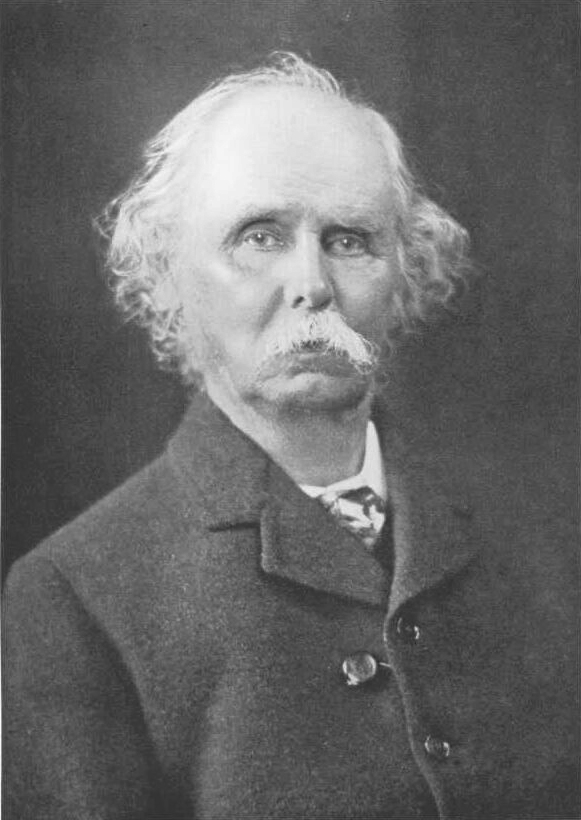
\includegraphics[width=0.5\linewidth]{img/intro/Alfred_Marshall} 

}

\caption{Image Sourced from Wikipedia.}\label{fig:intro02}
\end{figure}

The ordinary business of life:

\begin{itemize}
\tightlist
\item
  majors/minors in college
\item
  degree level
\item
  career
\item
  dating and marrying
\item
  vacations
\item
  having children or not
\item
  mortgage, renting
\item
  car payments, public transport
\item
  illness, elective surgeries
\item
  retirement, unretirement
\item
  etc, etc, etc, \ldots{}
\end{itemize}

All of these are parts of life for most of us, ordinary life.

One of the greats of modern economics, Partha Dasgupta\footnote{\url{http://www.econ.cam.ac.uk/people/emeritus/pd10000}}, writes

\begin{quote}
``These are no mere academic matters. If welfare and development economics, more generally political philosophy, are not about the circumstances in which people are born and the manner in which they are able to live and die, they are about nothing.''
\end{quote}

\begin{figure}

{\centering 
\includegraphics[width=0.5\linewidth]{img/intro/Partha_Dasgupta} 

}

\caption{Image Sourced from Wikipedia.}\label{fig:intro03}
\end{figure}

Evidently economics is about life from the moment we are born to the moment we die. With all its joys, with all its triumphs, but also with all its challenges, struggles, defeats and tragedies.

This includes the preemies that are born weighing less than 2 pounds with their and their parents' life-long struggle to flourish and to secure a comfortable life:

\begin{itemize}
\tightlist
\item
  How big are the medical bills?
\item
  Does insurance cover them all?
\end{itemize}

\begin{figure}

{\centering 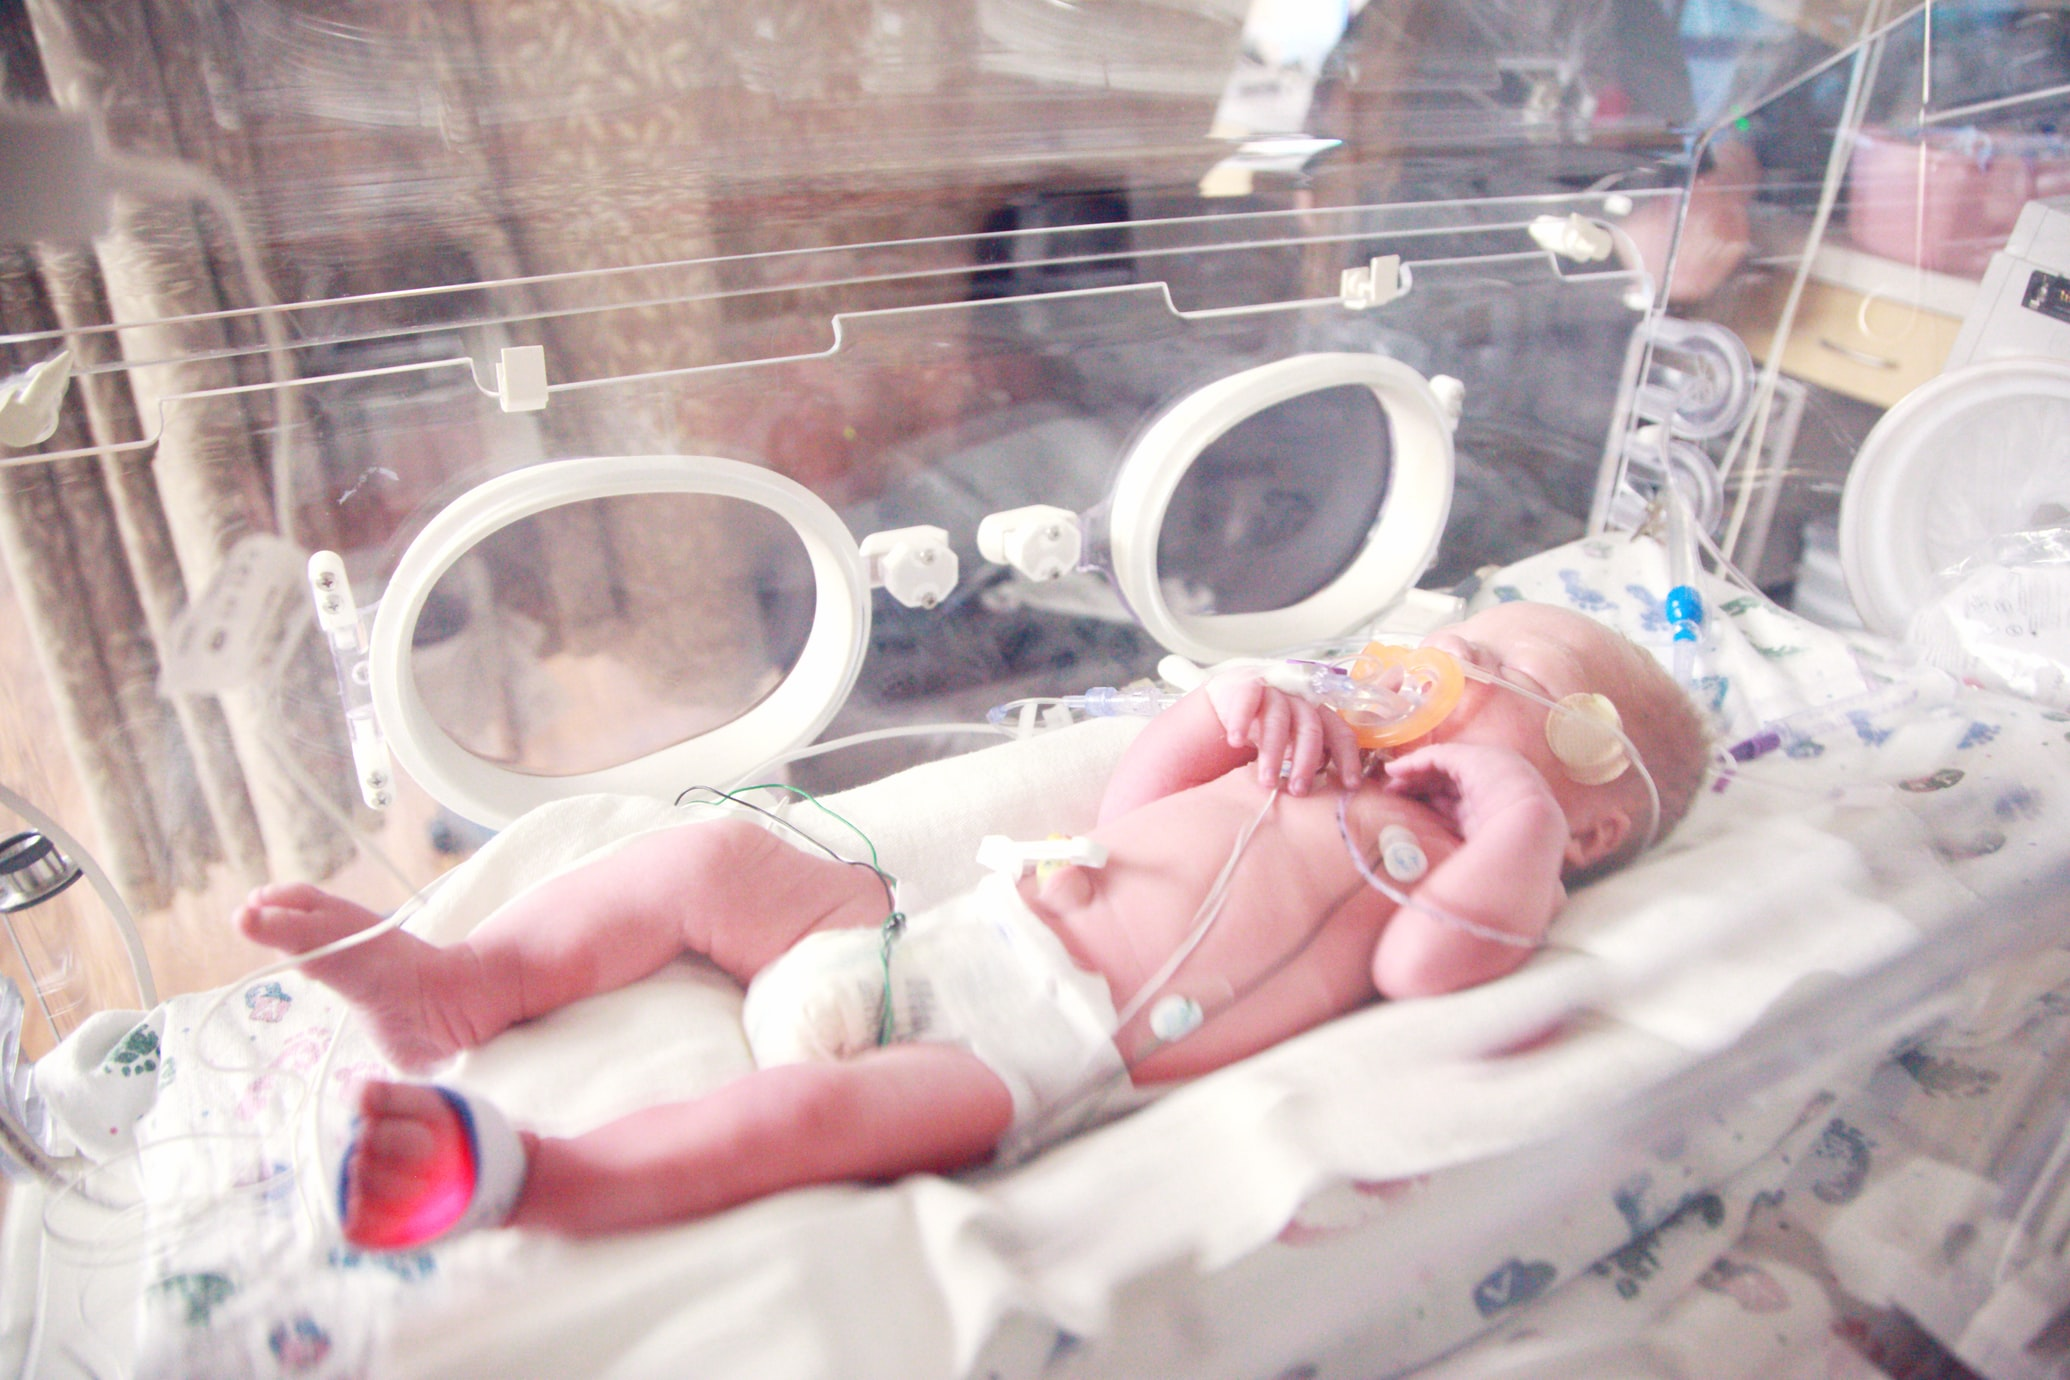
\includegraphics[width=0.5\linewidth]{img/intro/fig4} 

}

\caption{Image Sourced from unsplash.}\label{fig:intro04}
\end{figure}

This includes the child born in the ``wrong'' ZIP code area. The child that is developmentally behind at age 3, the child who will have a hard time catching up scholastically, the child who as a young adult will have difficulty making ends meet because of the poor employment prospects.\footnote{\url{https://research.upjohn.org/up_press/228/}}

This includes the person who was repeatedly abused as a child and who because of this experience faces a higher likelihood to be a part of the prison system later in life.\footnote{\url{https://www.nber.org/digest/jan07/does-child-abuse-cause-crime}} \footnote{For other consequences childhood abuse and trauma, see:
  \url{https://www.cdc.gov/vitalsigns/aces/pdf/vs-1105-aces-H.pdf}}

This includes the young person who graduated from college with huge student debt that is impossible to be paid back and that is very unlikely to be forgiven, even in bankruptcy.

This includes the parents of young children who are torn between going to work to pay the bills and staying home with their children because there is no reliable and safe childcare during COVID-19.

\begin{figure}

{\centering 
\includegraphics[width=0.45\linewidth]{img/intro/sadparentandchild} 
\includegraphics[width=0.45\linewidth]{img/intro/saddadandchild} 

}

\caption{Images sourced from unsplash.}\label{fig:intro05}
\end{figure}

This includes the retired college professor whose physician tells him:

\begin{quote}
``Walter, with your lung cancer you have 6 months to live, on the outside. Now is the time to do the things you've always wanted to do but have never done.''
\end{quote}

But who, the following morning, gets ready to go to his office, and when reminded by his wife of the physician's advice that now is the time to do the things he always wanted to do, replies:

\begin{quote}
``That is exactly what I'm doing. I am doing what I've always wanted to do. I am going to the office to do my work.''
\end{quote}

This includes the mother from Nicaragua, Guatemala, or Honduras, who flees with her children north, to what she thinks is a safer place for her children, knowing full well the meaning and implications for her of the term ``cuerpomatic'\,'\footnote{\url{https://www.americasquarterly.org/blog/rape-another-threat-on-migrant-womens-journey-north/}}.

\begin{figure}

{\centering 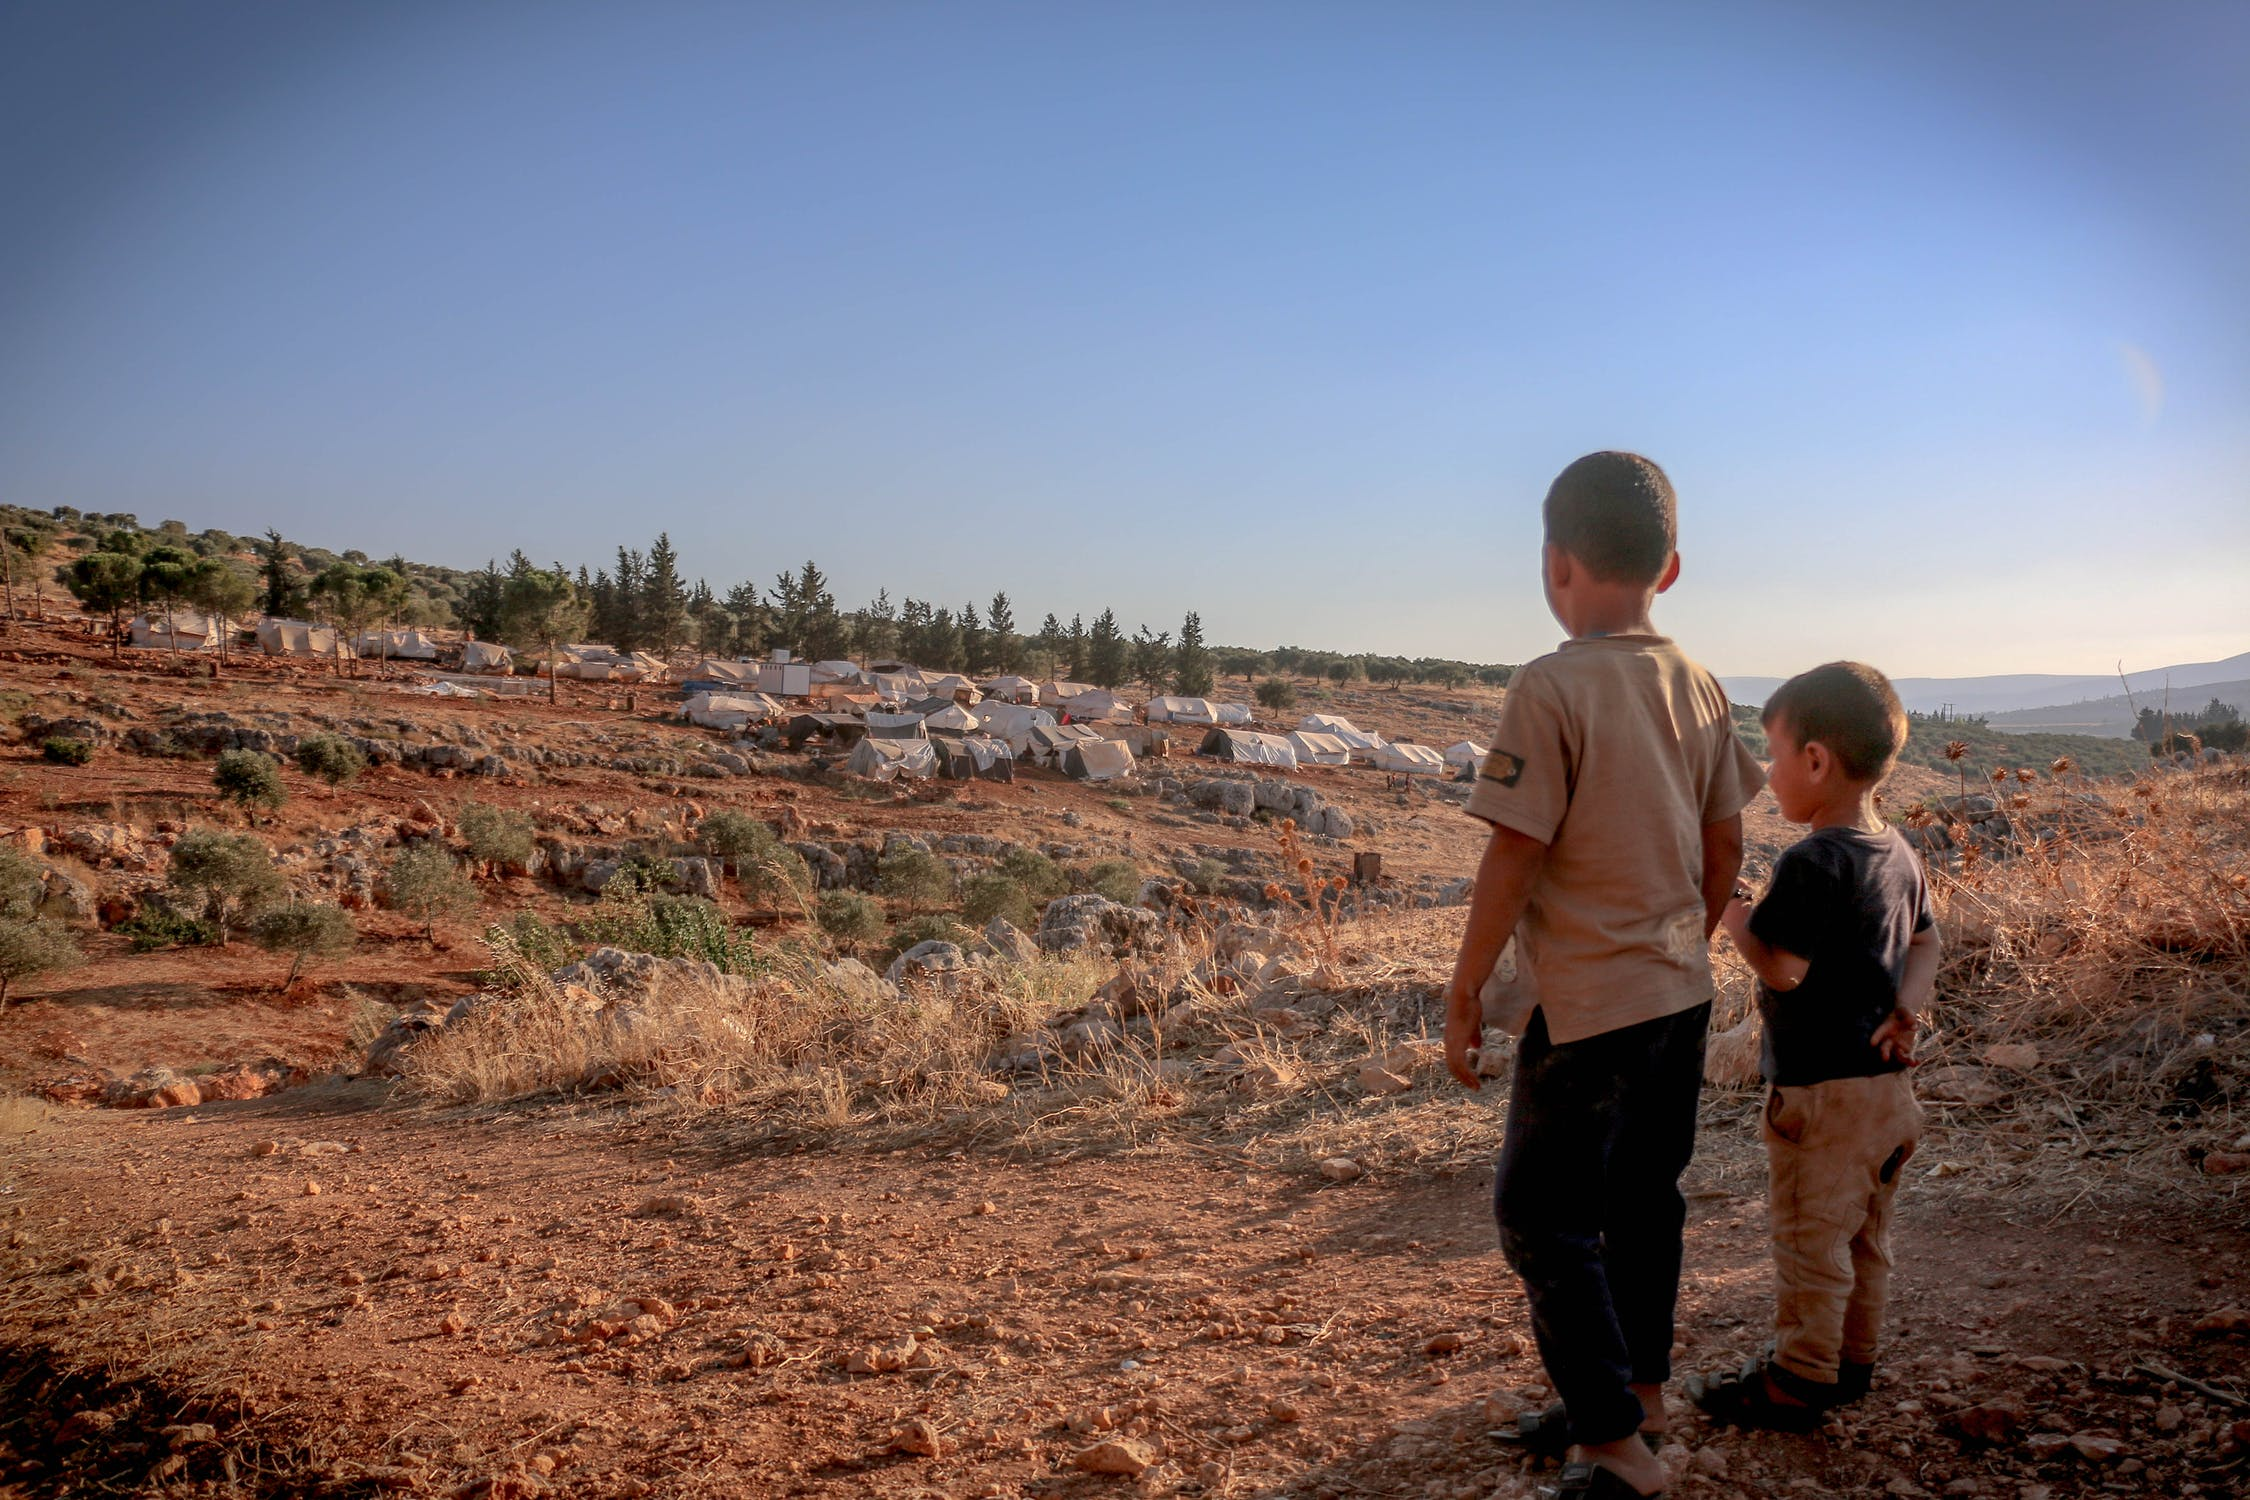
\includegraphics[width=0.7\linewidth]{img/intro/refugees} 

}

\caption{Image Sourced from pexels.}\label{fig:introrefugees}
\end{figure}

This includes things like positive assortative mating or ``like marries like''. Tall men/women tend to marry tall women/men. Another way of saying this is: The height of married couples is positively correlated. Highly educated women/men marry highly educated men/women. The level of education of married couples is positively correlated. The level of incomes are positively correlated.\footnote{\url{https://www.nber.org/system/files/working_papers/w19829/w19829.pdf}} It was not always like this.

This includes all those people who suffer from kidney failure, who are waiting for a transplant kidney, who may or may not get one. In this country, about 13 people die per day, because there are no transplants available.

\begin{figure}

{\centering 
\includegraphics[width=0.6\linewidth]{img/intro/kidneyfailure} 

}

\caption{Image Sourced from pexels.}\label{fig:introkidneyfailure}
\end{figure}

Most textbooks define economics to be the study of the allocation scarce resources. A resource here is simply a means, something that is useful. Useful for a purpose. We usually assume that people have goals or purposes and that they will try to achieve these goals. But there are constraints that stand in the way.

Money is resource that allows us to buy stuff. For most of us money is scarce, our budgets are limited. Therefore, we must make choices:

\begin{itemize}
\tightlist
\item
  The fancy car or a super vacation?
\item
  Paying the utility bill or paying the medical bill?
\item
  A fancy wedding or a dream house?\footnote{\url{https://www.netflix.com/title/81113929}}
\end{itemize}

\begin{figure}

{\centering 
\includegraphics[width=0.6\linewidth]{img/intro/emptywallet} 

}

\caption{Image Sourced from pexels.}\label{fig:introemptywallet}
\end{figure}

Time, perhaps our most valuable resource, is also scarce. You will surely notice this, as many have before you, during finals week. You will wish that there were five or six extra hours in each day.

\begin{figure}

{\centering 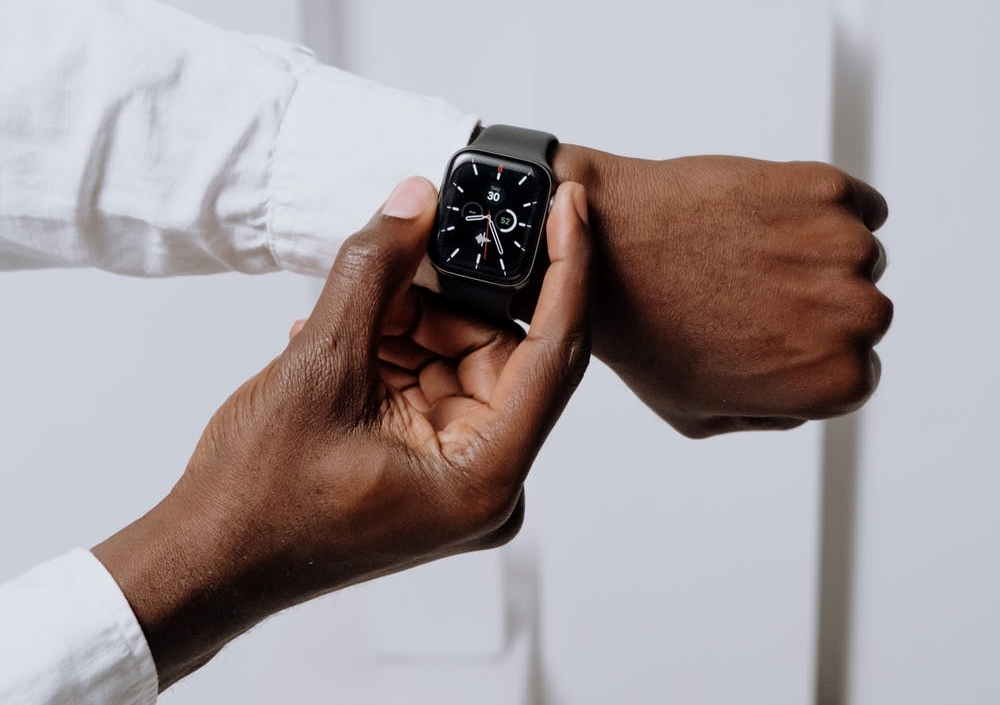
\includegraphics[width=0.6\linewidth]{img/intro/time} 

}

\caption{Image Sourced from pexels.}\label{fig:introtime}
\end{figure}

Bandwidth, our ability to compute, to calculate, to process information, to decide rationally, is surely limited and many of us wish that our bandwidth were much, much bigger.

For an illustration of big bandwidth see this scene from the movie Searching for Bobby Fischer\footnote{\url{https://www.youtube.com/embed/ybrY9JWVBv4?start=99}}

Many of us will, at some point hit emotional constraints. After strings of setbacks, failures, and disappointments, we will ask: ``How much more can I take?'' Suicide is arguably worst sign of emotional constraints, the ultimate of being at the end of one's rope. Suicides have grown considerably in the 50 States\footnote{\url{https://www.cdc.gov/nchs/data/nvsr/nvsr69/nvsr-69-11-508.pdf}}. There have been proposed policies which could decrease number of suicides\footnote{\url{https://www.nber.org/papers/w25787}}.

\hypertarget{what-is-economics-good-for}{%
\section{What is Economics Good For?}\label{what-is-economics-good-for}}

First and foremost economics, is a social science. We would expect economics to be good and useful in explaining behavior. When we look around, there are all kinds of interesting observations that we would like to explain. And economics can help us go a long way towards providing explanations for all kinds of behavior. Some examples where economics may have the potential to provide some explanations are:

\begin{itemize}
\tightlist
\item
  Why did grocery stores run out of toilet paper at the beginning of the COVID-19 pandemic?
\item
  Why did women suffer more than men from the COVID-19 induced epidemic when normally in other recessions men tend to suffer more employment losses than women?\\
\item
  Why are Dutch women taller than American women?
\item
  Why do women when they buy a house from a man pay a higher price than a man and when they sell a house to a man they get a lower price than a man?
\item
  Why did the price of bicycles rise during the COVID-19 recession?
\item
  Why did the price of used cars rise during the COVID-19 recession?
\item
  Why has the labor force participation of males been dropping for the last 20 or so years?
\end{itemize}

The question is always:
Why? Why? Why?

Perhaps we can spend a little bit of time thinking about the following three examples of observations and ask why did these things happen?

\begin{itemize}
\tightlist
\item
  In Maine in the 1800s, lobster was used commonly to feed prisoners and it was used often for fertilizer on the fields. Why?\\
\item
  In a recent 5K race in Bloomington, Indiana there were participants in basically all age groups from age 16 all the way up to age 80. This was true for both men and women with one exception. In the category Between age 30 and 35 there was not a single female participant. Why?\\
\item
  According to some reports from field workers in a refugee camp for the Rohingya in Bangladesh, there were children older than five years of age and younger than 2, but there were no children between the ages of 2 and 5. Why?
\end{itemize}

We will see how economics can provide answers too many of these why? why? why? questions.

Economics can also provide answers to questions like what are the underlying assumptions that some individuals make under which their behavior might be rational.

Many years ago I, Gerhard, was caught speeding. I was actually going quite fast, which is usually something I do not do. But we were quite late for a meeting and missing the meeting would have been very costly. So, driving at very high speed under these circumstances actually makes a lot of sense. It was the rational thing to do.

On May 25, 2020, Amy Cooper, a white woman, let her dog off its leash in Central Park, New York, despite New York City's leash law. Christian Cooper, a black male who was in the park watching birds asked her to leash her dog. Amy Cooper called the police alleging an ``African American man'' was threatening her. \footnote{\url{https://www.nytimes.com/2020/07/06/nyregion/amy-cooper-false-report-charge.html}}

Under what assumptions is the behavior of Amy Cooper in Central Park rational? \href{https://www.ncronline.org/news/opinion/assumptions-white-privilege-and-what-we-can-do-about-it}{This article} digs into this. Rationality here and in the rest of these notes means:

\begin{center}
\textbf{Our actions are guided by a particular purpose or goal, taking into consideration all constraints and all relevant information.}

\end{center}

Bryan Massingale in the article \href{https://www.ncronline.org/news/opinion/assumptions-white-privilege-and-what-we-can-do-about-it}{here} list many assumptions under which Amy Cooper's behavior in Central Park is actually rational. Her actions seem to make sense under the assumption, for example, that her word as a white female would have more weight than the word of a black male. Since she must have thought that any police officers, not a particular police officer, summoned by her would give more credibility to her word than to the word of a black male. She must have believed and hoped for what we would call systemic racism. Her actions make sense, her actions are rational, if she believes in systemic racism.

The second thing economics is good for is to evaluate policies. Policies are just the things institutions (or government in particular) do. The federal government determines spending on defense and Medicare. It regulates immigration to this country. The state government chooses educational policies and whether to legalize weed. A local government decides to fund public parks and bicycle paths. A country club determines the rules for the use of a golf course. A faith organization chooses particular youth programs. A corporation chooses particular human resources, HR, policies.

In each one of these cases we want to know:

\begin{itemize}
\tightlist
\item
  Does the policy work?
\item
  Is it a good policy?
\end{itemize}

We want to be able to hold public officials accountable for the policies they pick. In order to be able to do this, we need to be able to figure out how people respond and react to these policies.

This leads us to a subject that is covered in the opening chapters of basically all introductory economics textbooks:

\begin{center}
\textbf{the law of unintended consequences}

\end{center}

The law of unintended consequences simply states that when a policy is changed, people will respond to that policy change, and frequently in ways that are difficult to forecast by the policy maker. Of course, the more careful the policy maker thinks about possible responses of people to the change in the policy, the fewer surprise responses to the policy there will be. But it is a testimony to human ingenuity and creativity that even with the best intention the best laid plans of mice and men often lead to disastrous outcomes. My guess is that such adverse responses to policy changes will never be eliminated, even after the most careful analysis of the proposed policy change.

\hypertarget{unintended-consequences}{%
\section{Unintended Consequences}\label{unintended-consequences}}

It should not be a surprise that people will respond to changes in a policy. People simply do what they believe is in their best interest and when incentives change, chances are their behavior will change as well.

If I announce that in this class there will be a final exam that is comprehensive, that is the hardest exam on campus with a pass rate of only 30\%, there are a variety of possible student reactions to this kind of an announcement. Some students will decide to study harder, some students might get a tutor, some students might decide to come to office hours more frequently. Some students might just give up, drop the class and wait until that class is offered by a different faculty member who has easier exams. This is just incentives at work. But we have to acknowledge that different students will respond in different ways and it is just extremely difficult to predict the behavioral response of a particular student or particular groups of students.

There are some interesting examples to unintended consequences.

\hypertarget{unintended-consequences-examples}{%
\subsection{Unintended Consequences Examples}\label{unintended-consequences-examples}}

\textbf{(Epidemics I)} I, Gerhard, heard of a convenience store in Virginia that had attached to it a video arcade with a separate entrance. During COVID-19, the convenience store was declared essential and allowed to stay open, the video arcade shut by order of the government. How did the owner of the convenience store and the video arcade respond to this government policy? He simply moved some of the video games into the convenience store, thereby increasing the density of customers in the store. Chances are the risk of infection increased.

\begin{center}\rule{0.5\linewidth}{0.5pt}\end{center}

\textbf{(Epidemics II)} \footnote{\url{https://crofsblogs.typepad.com/h5n1/2020/05/trumps-europe-travel-ban-triggered-covid-19-spreadin-the-us.html}} On March 11, 2020, President Trump announced a travel ban from most countries in Europe to be effective March 13th and to last 30 days. If you are an American traveler in Europe, how would you respond to this announcement? If you are an American tourist in Europe, how would you respond? If you are an American on business in Europe, how would you respond? Or, if you are an American student on an exchange program how would you respond?

Regardless of your original plans for your return trip, you might well conclude that the best course of action for you is to hightail it home as quickly as you possibly can.

Evidently, many Americans decided that this was indeed their best course of action, so they changed their plans and returned home as quickly as possible. As a consequence, American airports on March 12 and 13 were overcrowded, contributing to the further spread of the virus. Perhaps this crowding might have been avoided to some degree by more carefully planning the return flights and spreading out the arrival of these flights over time.

\begin{center}\rule{0.5\linewidth}{0.5pt}\end{center}

\textbf{(Work Incentives)} During the financial crisis of 2008 and 2009, governments in many affected countries designed rescue packages in order to bailout banks, at least the largest banks. Some of these rescue packages contained explicit caps on bonuses for banking executives. If the government imposes caps on those bonuses, how might banks respond to such limitations? Well, if I cannot reward my employees through higher bonuses, I can still reward my employees by increasing their base salaries. To the extent that the bonuses are used to reward exceptionally good performances and thereby provide incentives for such exceptionally good performance, this cap on bonuses seems to have one adverse effect: weaker incentives for exceptional performance. Not sure if that is what you want.

\begin{center}\rule{0.5\linewidth}{0.5pt}\end{center}

\textbf{(Health)} Imagine you are concerned with excessively long waiting times at emergency rooms in the hospitals in your state. Suppose you want to design a scheme that rewards hospitals to decrease those waiting times. So, you collect the data on average waiting times in these emergency rooms and then you design rewards for those hospitals who reduce the waiting times the most. If you measure waiting time from the moment the patient comes through the door to the time the patient is treated, how might hospitals actually respond to this new policy?
Hospitals might ask the ambulances to wait in the hospital parking lot. Surely this is not a desired outcome.

\begin{figure}

{\centering \includegraphics[width=0.5\linewidth]{img/intro/ambulance} 

}

\caption{Image Sourced from unsplash.}\label{fig:introambulance}
\end{figure}

\begin{center}\rule{0.5\linewidth}{0.5pt}\end{center}

\textbf{(Education)} \footnote{\url{https://freakonomics.com/}} Supposed you want to reward teachers for better performances of their students on standardized tests. Suppose the stakes, the rewards are big. How might the teachers respond to these incentives? Surely there are many possibilities.

Some teachers might better prepare their lessons.

Some teachers might spend more time with students who are struggling.

But some teachers might also provide caffeinated sugary drinks to their students the day of the test to get a short time boost in attention and concentration to improve their performance. I suspect the dentists will love this.

Or, and this is an extreme case, some teachers might actually be induced to cheat on behalf of their students. One example of teachers engaging in such cheating is documented in the first book Freakonomics.

\begin{center}\rule{0.5\linewidth}{0.5pt}\end{center}

\textbf{(Gender)} \footnote{\url{http://ftp.iza.org/dp9904.pdf}} Family leave policies are intended to allow moms and dads to spend quality time with their new-born babies. In many places/organizations there has been a gradual shift from no leave, paid or unpaid, to maternity leave for the mom to family leave for both mom and dad, when a baby is born. In some organizations there is still no maternity or family leave policy in place and women have to take sick days or personal days to deliver their baby. At a typical university maternity or family leave is tied to ``stopping the tenure clock''. Stopping the tenure clock simply means, that mom and/or dad have extra time, often one year, to be considered for tenure. Tenure basically ensures lifetime job security. It is a BIG deal.

Allowing dads time off and stopping the tenure clock for dads as well as for moms is often seen as a great equalizer of men and women, dads and moms. After all, now dad can spend time with his baby as well. What could possibly be or go wrong with that?

The paper cited shows that the policy of providing gender neutral family leave and stopping the tenure clock in a gender-neutral way, increases dad's chances of tenure by 19 percentage points and decreases mom's tenure of tenure by 22 percentage points.

So much for achieving gender neutrality!

\begin{center}\rule{0.5\linewidth}{0.5pt}\end{center}

\textbf{(Gender II)} \footnote{\url{https://www.cesifo.org/en/publikationen/2020/working-paper/caught-between-cultures-unintended-consequences-improving}} The German government passed a law that grants automatic German citizenship rights to all immigrant children born in Germany after January 1, 2000. You might think that such a law would benefit all immigrants regardless of country of origin, skin color, religion, sex, gender identity and age. Why? It is just a right. The law increases the realm of the possible. It increases opportunities. It does not take away any opportunities. What could possibly be wrong with more choices, more opportunities? So, one would be inclined to think that all immigrants would be better off and report being happier. And in that believe we would be wrong. Why? The law of unintended consequences strikes again.

Self-reported happiness declined after this law was passed for Muslim girls. Muslim immigrant girls become disillusioned. Muslim parents are less likely to help their daughters who qualify for citizenship with their homework. They are also less likely to speak German with their daughters. Muslim immigrant girls who qualify for German citizenship are less likely to self-identify as German.

The law of unintended consequences truly rears its ugly head.

None of these effects are found for Muslim boys. None of these effects are found for children of other faiths.

Why do we find these effects for Muslim immigrant girls? Parents of Muslim immigrant girls react strongly to counteract the pull of German society to keep their daughters withing their cultural and religious traditions.

\hypertarget{exercises}{%
\subsection{Exercises}\label{exercises}}

\begin{enumerate}
\def\labelenumi{\arabic{enumi}.}
\item
  Suppose a state government passes a law that allows for ``No knock warrants''. \href{https://en.wikipedia.org/wiki/No-knock_warrant\#:~:text=In\%20the\%20United\%20States\%2C\%20a,knocking\%20or\%20ringing\%20a\%20doorbell}{See here} if you are unsure what this is.

  A. Make a list of the possible ``unintended consequences'' of this policy.\\
  B. Who would get impacted by this policy? Positively or negatively?\\
  C. How hard is it to foresee/forecast these consequences?
\item
  President Trump issued an Executive order on June 22, 2020 to severely limit H1-B and L1 visas. H1-B visas are visas issued so American companies can hire high-skilled immigrants. L1 visas allow American multinational corporations to transfer foreign managers and employees to their offices in the US. \footnote{\url{https://www.nber.org/papers/w27997}}

  A. Make a list of all the effects of this policy. Who would get impacted by this policy? Positively or negatively?\\
  B. How hard is it to foresee/forecast these consequences?
\end{enumerate}

\hypertarget{role-of-theory}{%
\section{Role of Theory}\label{role-of-theory}}

What is the role of theory in economics?

\begin{figure}

{\centering 
\includegraphics{introeconfull_files/figure-latex/intropeterthinker-1} 

}

\caption{Images sourced from wikimedia commons. Statues of The Thinker and Peter Abelard.}\label{fig:intropeterthinker}
\end{figure}

A quote by a 12th century philosopher, Peter Abelard:

\begin{quote}
``The man of understanding is he who has the ability to grasp and ponder the hidden causes of things. By hidden causes we mean those from which things originate, and these are to be investigated more by reason than by sensory experiences.''
\end{quote}

We can paraphrase this by saying: If we want to understand stuff, we ought to rely more on our brain and think more about how things might actually work, rather than collecting data with our senses.

Charles Darwin, in a letter to one of his friends expressed a similar opinion:

\begin{quote}
``About thirty years ago there was much talk that geologists ought only to observe and not theorise; and I well remember someone saying that at this rate a man might as well go into a gravel-pit and count the pebbles and describe the colors. How odd it is that anyone should not see that all observation must be for or against some view if it is to be of any service!''
\end{quote}

\begin{figure}

{\centering 
\includegraphics{introeconfull_files/figure-latex/introdarwinpebbles-1} 

}

\caption{Image sourced from wikimedia commons.}\label{fig:introdarwinpebbles}
\end{figure}

\begin{center}
\textbf{Go enjoy counting the pebbles!}

\end{center}

I interpret that last clause in Darwin's letter to mean: All observations must be used to either confirm or reject a hypothesis or theory, if the observation is to be of any use at all. That implies that theory comes first.

So, what is this thing called a ``theory''? I will use the words: theory, model, and abstraction synonymously. A theory is a creation of our minds; it is an idea of how some part of the word operates or might operate.

Theories used in economics will be different than in theories used in physics. Even within economics there will be different theories or models. Macroeconomists will use different models than economists who study anti-trust. The main job of a model is to help us understand how a part of the world works. Any theory or model is supposed to be useful, for understanding.

\hypertarget{abstractions}{%
\subsection{Abstractions}\label{abstractions}}

How is an abstraction useful? Suppose the job is to drive from Indianapolis, IN to Columbus, OH. We need a map to help us get there.

\includegraphics[width=0.75\linewidth]{img/intro/mapshot}

Above we have a map. It has all kinds of information. A bunch of cites like Detroit, Gary, Fort Wayne, Cincinnati. State Forests, State Parks. Lake Erie, Lake Michigan. Much of this information is not relevant if the task is to get from Indianapolis to Columbus.

In order to get from Indianapolis to Columbus, not much information is needed. Most, practically all of the information above is useless and needs to be discarded. Pretty much the only information needed is illustrated below. All we need is the starting point, Indianapolis, the endpoint, Columbus, and the instructions to get on I-70 in Indianapolis until the sign ``Columbus, OH'' appears. This is really all that is essential.

Indianapolis---------------------------I 70---------------------------------Columbus

There are a few more things that one might reasonably add to our ``model'' of the relevant piece of geography. It might be useful where the gas stations are, especially the ones with clean bathrooms, and where the coffee shops are so the driver does not fall asleep. One such establishment, marked by G for gas station, is added in the model below.

Indianapolis---------------------------I 70--------------------G-----------Columbus

\hypertarget{prejudice-based-wage-discrimination}{%
\subsection{Prejudice-Based Wage Discrimination}\label{prejudice-based-wage-discrimination}}

How to find prejudice-based wage discrimination?

In this example we will try to show that economic theory can generate useful insights or knowledge. The way this works in this example is that economic theory will suggest precisely where we have to look for evidence. The issue or example that we will use here is the question:
How, if, and to what extent does racial prejudice show up in, or generate wage discrimination by race?

The work in economics on racial discrimination goes back at least to the seminal work by Nobel Laureate Gary Becker from the University of Chicago\footnote{The Economics of Discrimination by Gary Becker (1957)}.

For starters, we have to distinguish between prejudice and wage discrimination. Prejudice is an attitude, a negative attitude, a sentiment toward a particular group of people, Blacks for example. Wage discrimination is a particular outcome in labor markets that simply says comparable blacks and comparable whites receive different wage rates.

The question then is: How, to what extent, if at all, does racial prejudice determine such wage discrimination?

In order to start thinking about this issue, we will consider a very simple example. Blacks make up about 10\% off the population or the labor force. There are two distinct labor markets. In labor market 1 the population of white people exhibits basically no racial prejudice. In labor market 2, the population of white people exhibits very strong racial prejudices.

In which labor market would we expect wage discrimination by race to be strongest? Labor market 1 or labor market 2?

Without a moment's thought most of us would be tempted to say: Of course, racial discrimination is higher, stronger, worse in labor market 2 than in labor market 1.

But that would be missing an element of the story that probably is very important.

Blacks will most likely know or at least have some pretty good information on where the racists live, in which labor market they operate. Why would they know this? Chances are they have experienced the manifestations of racism and through their social network this information is broadly shared.

So, to the extent that blacks have information on manifestations of racism and to the extent that they are free to move between labor markets, to choose their place of employment, they will probably move from labor market 2 to labor market 1. This is of course, is with holding other things equal. Holding other things equal just means that in all other aspects these two labor markets are roughly comparable. They only differ in this one aspect: prejudice.

So, if blacks can move freely, relatively freely, they will choose labor market 1 over labor market 2 in which case there might be very little racial wage discrimination in labor market 2. If all Blacks where to move into labor market 1, then there would be no racial wage discrimination in labor market 2 at all.

Therefore, our answer that labor market 2 will exhibit more wage discrimination than labor market 1 is probably false.

There is a \href{https://papers.ssrn.com/sol3/papers.cfm?abstract_id=1073644}{recent paper linked here}, together with a short video by one of its authors below, that uses currently available data to show us exactly where and how we should look for the impact of prejudice on labor market discrimination.

We start with constructing a racism distribution. This is not just some fancy Ivory Tower notion. This distribution is firmly grounded in data. There is a data set that is widely available, called The General Social Survey, GSS, that asks questions like:

\begin{figure}

{\centering 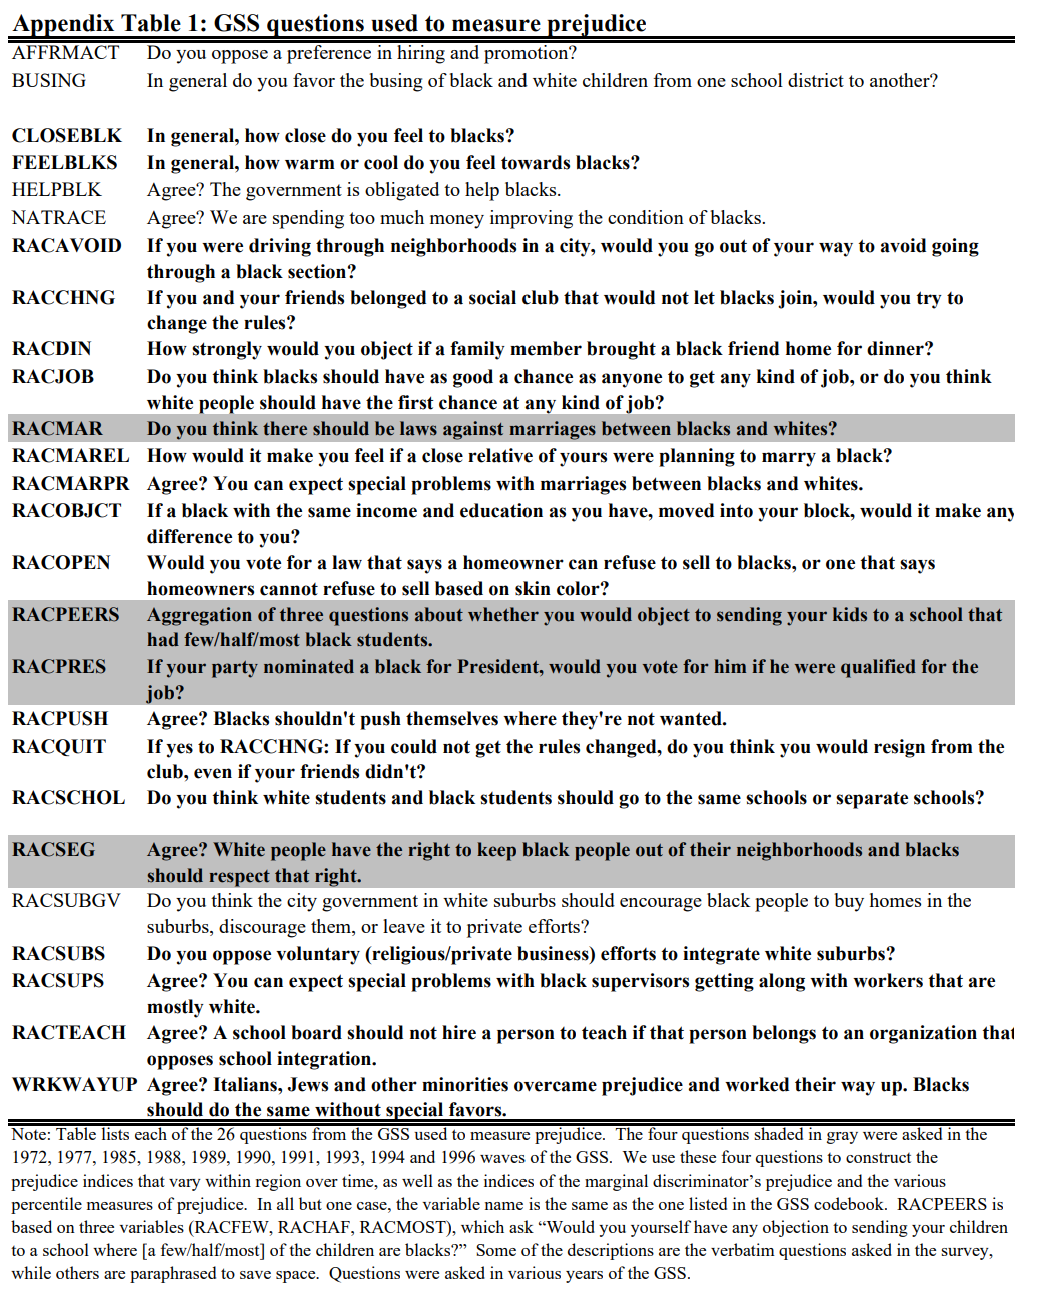
\includegraphics[width=0.8\linewidth]{img/intro/gssquestions} 

}

\caption{Table from Prejudice and the Economics of Discrimination by Kerwin Kofi Charles and Jonathan Guryan.}\label{fig:gssquestions}
\end{figure}

The authors use only the questions in bold for their purposes since the non-bold questions might elicit answers that are not purely guided by racist sentiments.

Answers to questions like these can be put together to create an index of racism and then a distribution of racism in a particular locality. The figure below illustrates such an example off a racism distribution.

\begin{center}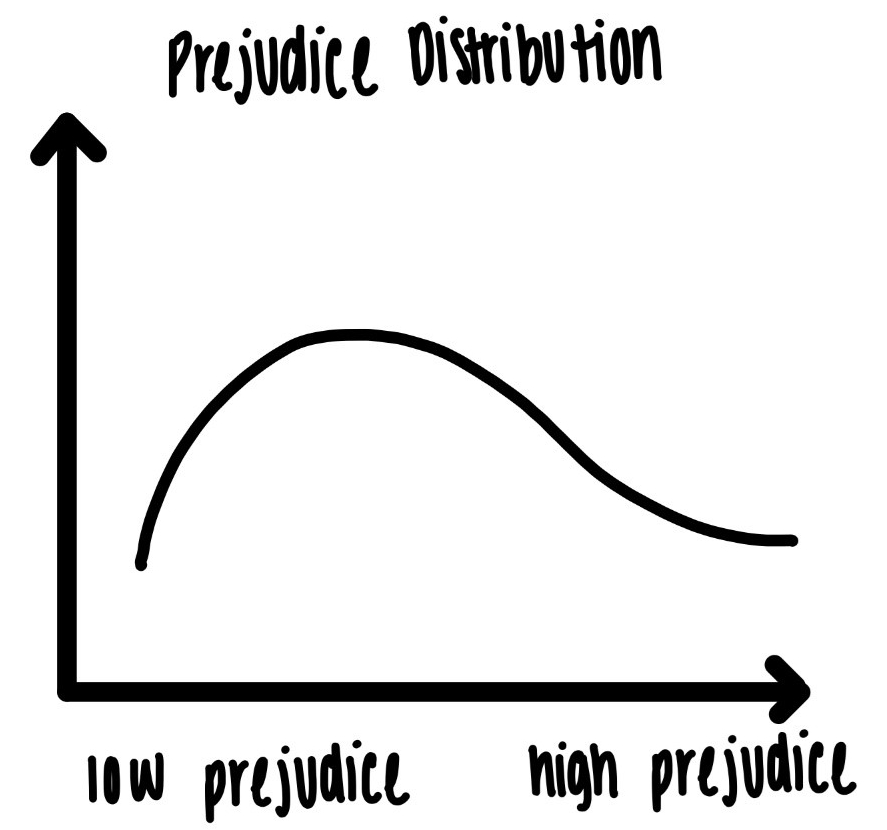
\includegraphics[width=0.6\linewidth]{img/intro/prejdist} \end{center}

Some researcher suggests that in order to assess the impact of prejudice on wage discrimination one should look at a correlation between the average or median degree of prejudice and the average level of wage discrimination. They collect the best data available for the 50 States and calculate or estimate that correlation. They find nothing.

Why?

Just like in the example with 2 labor markets, Blacks will, if they can, avoid the right tail of the racism distribution. It is certainly in their interest to do so. They will shift to the left, i.e.~seek employment, as far as possible in the racism distribution.

In Wisconsin, about 6\% of the labor force is black. If they all seek employment, they would be matched with some, mostly likely white, employer. If we line up all white employers on a racism distribution, with the least racist employers on the left and the most racist employers on the right, then black workers would seek employment as far away from the most racist employers as possible. Black workers would go to the left of the racism distribution as much as possible. Since Blacks in Wisconsin make up 6 percent of the population, these 6 percent would then be seeking employment from the 6 percent of the least racist employers. Since Blacks are seeking employment as far to the left tail of the prejudice distribution as possible, then it is the 6 percentile of the prejudice distribution that matters for wage discrimination. Not the average, not the median. The 6th percentile.

In Mississippi, about 34\% of the labor force is black. In Mississippi, wage discrimination is determined by the 34th percentile of the prejudice distribution. Not the average, not the median, not the 6th percentile. The 34th percentile.\footnote{See Appendix for a refresher on percentiles}

So far, we have not looked at any data; so far this is all theory.

What is in the data?

When you look for the connection between prejudice and wage discrimination by looking at averages you find nothing.

But when you look for it in the way suggested by the theory, the 6th percentile of prejudice distribution in WI, the 34th percentile in MS, then BINGO! There it is, clear and significant evidence linking prejudice to wage discrimination. You just need to know where to look. Theory helps.

\hypertarget{dealing-with-data}{%
\section{Dealing with Data}\label{dealing-with-data}}

\hypertarget{empirical-regularities}{%
\subsection{Empirical regularities}\label{empirical-regularities}}

First of all, we note that we are more interested in empirical regularities rather than in singular observations. Jennifer being 5'4'' is an example of a singular observation. That is only one observation. ``Dutch women are tall'' is an example of an empirical regularity. More precisely the average height of Dutch women is 5'7'', compared to the average height of American women which is 5'4''. This observation is more general. We would find this if we looked at a sample of women from Amsterdam, from Rotterdam, from The Hague, etc.

Rich people live longer than poor people.

This is a fact, in Indiana, New Jersey and in Kentucky. It is also true in France and in Japan.\footnote{\url{http://www.equality-of-opportunity.org/assets/documents/healthineq_summary.pdf}}

The sex ratio in the US is 1.04. The sex ratio is the ratio of the number of women to the number of men. For each 100 men in this country there are 104 women. If you look up this ratio by State, there is some variation. For most states, there are more women than men. But there are exceptions. In some Western states, there are more men than women. These exceptional states include Alaska, Montana, Wyoming. You may want to ask why there are such large differences in sex ratios across the 50 States.

\textbf{Numbers: Big or small?}

One of the important issues we have to discuss is: Are numbers big or small. This is especially true when we are talking about dollars, taxes, expenditures, the size of government programs.

\hypertarget{examples}{%
\subsubsection{Examples}\label{examples}}

\textbf{(Earthquake Relief)} After the Haiti earthquake in 2010, the US government committed \$100 million in earthquake relief. Big number or small number? It might look like a big number. But when you consider that there are over 300 million Americans, we realize that each of us gave about 30 cents, which looks miserly. Of course, this does not include private charitable contributions.

\begin{center}\rule{0.5\linewidth}{0.5pt}\end{center}

\textbf{(Apollo Mission)} \footnote{\url{https://www.whitehouse.gov/briefings-statements/white-house-seeks-billions-record-investments-stop-drug-epidemic/}} The cost of the Apollo mission which ultimately landed a man on the moon has been estimated to be about \$150 billion dollars, (adjusted for inflation) in 2019 dollars. In 2019, the White House made a request to combat deaths from illicit opioid abuse to the tune of \$7 billion. In 2021 over 100,000 people died from drug overdoses. Is \$7 billion a big number or a small number?

\begin{center}\rule{0.5\linewidth}{0.5pt}\end{center}

\textbf{(Vaccine R\&D)} According to an article in The Economist, August 8-14, 2020 world- wide spending on research for a COVID-19 vaccine was about \$10 billion. Sure sounds like a heck of a lot of money. But! Just in the US, the number of people who have died, at that time, was about 100,000. At the time of this writing that number has surpassed 900,000 COVID-19 deaths. The value of a statistical life\footnote{Kip Viscusi \url{https://law.vanderbilt.edu/bio/w-kip-viscusi} pioneered the research on the value of a statistical life.} in the US for the median age American is about \$10 million. Since COVID-19 takes mostly older people we might use \$5 million for the value of an older statistical life. The typical failure rate in late stages of vaccine trials is about 20\%. Multiplying the value of an older statistical life by the number of Americans who died because of COVID-19 we get:

\[ \$100,000 \times 5 \times 1,000,000 = \$ 500 \ \ \text{ billion} \]

COVID-19 does not only kill Americans. We now know that the death toll is much higher. The question is: Is the \$10 billion expenditure noted above a big number or a small number? Or: Should we have spent more on vaccine research in 2020?

\hypertarget{correlation-vs-causation}{%
\subsection{Correlation vs Causation}\label{correlation-vs-causation}}

This distinction is crucial. Knowing whether 2 variables are correlated is useful, but it is not enough. In order to make any kind of policy decision we must know causation. Correlation only tells us about a statistical relationship. Two variables may be positively correlated or they may be negatively correlated. Suppose variable X is positively correlated with variable Y. Then if X is large (small), then Y is large (small) as well. If the two variables X and Y are negatively correlated, that means that If X is large (small), then Y is small (large). Of course, there is also the possibility of no correlation.

\begin{itemize}
\tightlist
\item
  Our typical calorie intake is positively correlated with my body weight.
\item
  The time students spend studying for Finite Math exams may be negatively correlated with the grades in English classes.
\item
  Whether students are vegetarians or not is (I suspect) not correlated with their grades in introductory History classes.
\end{itemize}

We can think of these correlations as patterns in the data. They tell us nothing about causation.

Causation is an altogether different story. Causation means that one event leads to another. The event ``An increase in the price of socks'', will lead to the event ``I buy fewer socks''. We will talk about this at some length in this class.

The event ``90 percent of Americans getting the COVID-19 vaccine'' will lead to the event ``Americans achieve herd immunity''. Is this a dream?

The event ``Driving like a maniac on the interstates'' leads to the event ``The probability of fatal car crashes rises''.

There are lots and lots of examples like this. We need to be able to infer causality if we want to have any hope that the policies we pick actually make things better.

If two variables, X and Y, are positively correlated, there are several possibilities concerning causation:

\begin{enumerate}
\def\labelenumi{\arabic{enumi}.}
\tightlist
\item
  X could cause Y: an increase in X could cause an increase in Y. An improvement in nutrition in childhood causes an increase in adult height. There is no way adult height could influence the quality of childhood nutrition.
\item
  Y could cause X: an increase in Y could cause an increase in X. An improvement in nutrition in childhood causes an increase in adult height. There is no way adult height could influence the quality of childhood nutrition. (noticed this is just the same example as 1.)
\item
  X could cause Y AND Y could cause X: You study hard for your econ class and as a consequence you do well in the class. And: Since you do well in your econ class, you like econ and therefore you study harder. The hard part might be to find out which effect is stronger.
\item
  X does not cause Y, nor does Y cause X. But there is another variable, Z, that causes both X and Y. Education and smoking are negatively correlated. Typically people with many years of education are less likely to be smokers. It might be the case that education does not cause smoking. It is hard to imagine that smoking has a causal effect on education. The variable Z that causes both education and smoking is the underlying degree of patience. If I am very patient I can put up easily with an annoying econ teacher in the hope of getting high rewards from education, even in the distant future. If I'm not patient, I need that cigarette now, even if I am well informed about the high risk of dying from lung cancer 30 years down the road.
\end{enumerate}

In order to tease causation out of the data, we try to create what we call {\textbf{a parallel universe.}}

The point of this parallel universe is to look at two cases, two ``universes'' that are equal in all aspects except one aspect, the aspect we want to study.

\hypertarget{examples-1}{%
\subsubsection{Examples}\label{examples-1}}

\textbf{(Stand Your Ground)} \footnote{\url{https://jamanetwork.com/journals/jamainternalmedicine/fullarticle/2582988}
  For more comprehensive evidence, see
  \url{https://www.rand.org/research/gun-policy/analysis/stand-your-ground/violent-crime.html}} Suppose I want to study the effect of the Florida ``stand your ground law'' on homicides in Florida. Then I will collect all kinds of data for Florida. And I will collect the same kind of data in similar states. It would make little sense to compare Florida to Norway. But comparing Florida to states with similar income distribution, similar ethnic composition, similar poverty rates, similar age distribution makes sense. Like Georgia, Alabama, Arkansas.

Then we can compare homicide rates in Florida to those in other states that did not pass stand your ground laws. That is one difference we can exploit for our analysis. The other difference we can exploit for our analysis is to what happened to the trend in homicides before and after the law was passed.

The conclusion that emerges in this case is quite shocking: It appears that the stand your ground law has caused an INCREASE in homicides.

\begin{center}\rule{0.5\linewidth}{0.5pt}\end{center}

\textbf{(Gender II Revisited)} \footnote{\url{https://www.cesifo.org/en/publikationen/2020/working-paper/caught-between-cultures-unintended-consequences-improving}} In the \textbf{Gender II} example in the Law of Unintended Consequences examples above, how could the researchers ``establish'' or ``find'' a parallel universe? Sometimes you are just lucky. The law applied to all immigrant children born after January 1, 2000. The law separates those immigrant children born before that date from those born after that date. Children borne 6 months before and children borne 6 months after will be in the same school grade. They will be very, very similar in all or at least most other aspects. The fact that the law kicks in January 1 is very fortuitous for researchers. It creates almost ideal conditions to have a treatment group and a control group. Having a treatment group and an identical control group is what we mean by having ``a parallel universe''.

\begin{center}\rule{0.5\linewidth}{0.5pt}\end{center}

\textbf{Plastic Bag Ban} \footnote{\url{https://www.nber.org/papers/w28499}} In 2015, the City of Chicago banned all single use plastic shopping bags that were less than 2.25 mils thick. All other bags were unregulated. What are the consequences of this ban?

Short answer: Stores responded by using bags that are still made of plastic and that are thicker and therefore use MORE plastic. Another unintended consequence.

Unintended consequences seem to be everywhere.

How would we know? How can we infer causality? Where are the parallel universes? Where are treatment and control groups?

The researchers reasoned that stores just inside city limits ought to be very similar to stores just outside the city limits in the suburbs. The researchers also reasoned that shoppers just inside the city limit are very similar to shoppers just outside the city limit. So, data from just outside the city limit can serve as a parallel universe to what is going on inside the city limit.

There is more: Stores and shoppers just before the ban and just after the ban are going to be very similar. So, in addition to the comparison of inside and outside the city limit we have the comparison of just before and just after the ban. Looking at these two comparisons allows the researchers to nail down the effect of the ban: Disposable bag use remained very high. Many grocery stores just used bags that were just thick enough to be above the limit.

\begin{center}\rule{0.5\linewidth}{0.5pt}\end{center}

\textbf{(Health Effects of Lead)} \footnote{\url{https://www.economist.com/united-states/2021/04/17/replacing-lead-pipes-a-newark-success-story}} \footnote{\url{https://www.nber.org/papers/w27996}} How damaging to your health is lead? This is a big question. Most rich countries have tried to eliminate lead from gasoline and from paint. Lead is often still found in drinking water. How does lead get into your drinking water? Through the lead pipes.

We can narrow down the question a bit: How damaging is lead from drinking water to your baby's health?

The paper below provides an answer by considering a natural treatment and control group, or, in our language, a parallel universe. We find the parallel universe in Newark, NJ. The city was served by two different water treatment plants, with the service boundary of the two plants being basically an arbitrary line running across the city. An accident (bad decision?) in one treatment plant caused excessive corrosion and, as a consequence, excessive exposure to lead in one part of the city. This excessive exposure to lead increased the probability of low birthweight babies by between 1.4 and 1.9 percentage points. This is an increase of between 17 and 22 percent.

Exploiting such parallel universes can, evidently, be quite useful.

\hypertarget{glossary-of-terms}{%
\section{Glossary of Terms}\label{glossary-of-terms}}

\textbf{Causation:} one event leads to another or that a change in one variable leads inexorably to a change in another variable.

\textbf{Correlation:} describes the linear relationship between two variables. It is normalized to take values between +1 and -1. This is only a description of the relationship between two variables. It has no implications for causality.

\textbf{Constraint:} a limit on what is possible. Eg: financial, physical, emotionally, etc.

\textbf{Law of Unintended Consequences:} any action, any change in a policy or in a rule is bound to have consequences which are difficult to foresee before or when the action or change in policy or rule is put into place.

\textbf{Parallel Universe:} a scenario in which data sets would be equal in all dimensions except the one that we are studying. This is in order to determine causality.

\textbf{Scarcity:} available resources falling short of the wants, needs, or desires of people

\textbf{Theory:} a mind construct of how a part of the world may work. The point of a theory is to help us understand that part of the world. A synonym for theory is ``Model''.

\hypertarget{practice-questions}{%
\section{Practice Questions}\label{practice-questions}}

\hypertarget{discussion}{%
\subsection{Discussion}\label{discussion}}

\begin{enumerate}
\def\labelenumi{\arabic{enumi}.}
\tightlist
\item
  Can you think of an example from your personal life where you made a decision with the best of intentions that lead to unintended adverse consequences? Why did these consequences happen?
\item
  A university professor announces on the first day of class that the final exam in the class will be the hardest exam the students will ever face. How might students respond to this announcement? How would you respond?\\
\item
  The Federal government announces that international students are not allowed to enter the country if the university of their choice is teaching 100\% of its classes online. How might universities respond to this announcement?
\item
  The US government prohibits the importation of fentanyl into the US. How might the international suppliers of fentanyl respond to this policy?\footnote{\url{https://www.npr.org/2020/11/17/916890880/we-are-shipping-to-the-u-s-china-s-fentanyl-sellers-find-new-routes-to-drug-user}} \footnote{\url{https://www.politico.com/news/2022/02/08/synthetic-drug-trafficking-opioids-00006517?cid=apn}}
\item
  When does the world run out of oil?
  The known reserves of oil underground world-wide is 531,000,000,000 barrels. The annual consumption of oil word-wide is 16,500,000,000 barrels. Given these two numbers, when will the world run out of oil. What theories/models, assumptions did you use to arrive at your conclusion?
\item
  In your own words, explain why theories have to be abstractions. Provide one example of a theory not mentioned in class that is an abstraction and useful.
\item
  Provide a theory of why men are taller than women.
\item
  Provide a theory of why Dutch women are taller than American women.\\
\item
  Why was Italy the first European country to experience a major COVID-19 outbreak?
\item
  Can you provide an example of a model that is false, but useful? What is the model used for? Why is that model false?
\item
  Why are there more women alive in the US than men?
\item
  Provide a list of statements you have heard that are ``not even false''.
\item
  Imagine you obtain data on how many hours Indiana University students study for Finite Math and their grade in Introductory English. Would you expect these two datasets to be positively or negatively correlated. Explain.
\end{enumerate}

\hypertarget{multiple-choice}{%
\subsection{Multiple Choice}\label{multiple-choice}}

\begin{enumerate}
\def\labelenumi{\arabic{enumi}.}
\item
  A theory is

  A. An abstraction\\
  B. Realistic\\
  C. Consistent with observations\\
  D. Verifiable
\item
  A university professor announced on the first day of class that the final exam in her class is the hardest final the students will ever have on campus and that the pass rate on that exam is typically about 35 \%. The following are ways students might respond to this announcement.

  A. Some students will drop the class\\
  B. Some students will decide to study harder for the final\\
  C. Some students study habits are unaffected by this announcement\\
  D. All of the above
\item
  Economics can be considered the study of the allocation of \_\_\_\_ resource.

  A. Ample\\
  B. Scarce\\
  C. Sufficient\\
  D. Abundant
\item
  Hermannus goes on nice vacation along the Norwegian fjords. The price of the vacation is \(\$2000\). While on vacation Hermannus forgoes his income being a tutor for medieval German. That forgone income is \(\$500\). Hermannus' opportunity cost of the Norwegian vacation is

  A. 0\\
  B. 500\\
  C. 2000\\
  D. 2500
\item
  In the 1800s in Maine, lobster was used for fertilizer. Why?

  A. It was widely available compared to other fertilizer options\\
  B. It was more expensive than other fertilizer options\\
  C. It was harder to obtain than other fertilizer options\\
  D. Your TA likes lobster
\item
  The country of Superintelligentia wants to improve educational outcomes. To that end the country decides to provide special rewards to teachers if their students perform well on national standardized tests. Which of the following is probably not a consequence of this policy reform?

  A. Teachers try to cheat for their students\\
  B. Teachers offering extra tutoring help for their students\\
  C. Teachers working harder to prepare their classes\\
  D. Teachers retiring early
\item
  The law of unintended consequences

  A. Is of no practical consequence\\
  B. Is becoming less and less important as we have more and more date to analyze\\
  C. Is a reflection of our incomplete understanding of human behavior\\
  D. Was passed by the State Legislature of Indiana in 1982.
\item
  A country is spending \(\$10\) billion on research for an effective coronavirus vaccine. That vaccine, could save potentially 50,000 people. If the value of a statistical life is \$ 5 million, then

  A. The country should spend more on research\\
  B. The country should spend the same amount on research\\
  C. The country should spend less on research\\
  D. The country should ask Brazil to fund research
\item
  The mythical country of Cleanlandia annually spends \$ x on enforcing legislation that keeps their air clean. You could determine whether that expenditure is large or small by

  A. Calculation the expenditure on similar enforcement in that country 50 years ago\\
  B. Calculating the equivalent expenditure in some other country\\
  C. Calculating that expenditure per inhabitant of Cleanlandia\\
  D. Calculating that expenditure in Canadian dollars
\item
  The point of creating ``a parallel universe'' is to

  A. Detect a correlation between two variables\\
  B. See a pattern in the data\\
  C. Create a stimulating environment for video game games\\
  D. Detect causation in two related variables
\item
  The point/goal of a theory/model is

  A. To be realistic\\
  B. To be mathematically elegant\\
  C. To help understand the complex relationships between variables\\
  D. To be as general as possible
\item
  When teachers are rewarded through bonuses or higher salary increases for higher test scores of their students, teachers

  A. Have an incentive to seek employment in schools with more gifted students\\
  B. Have an incentive to cheat on behalf of their students\\
  C. Feed sugary caffeinated drinks to their students\\
  D. All of the above
\item
  A theory should be

  A. general\\
  B. elegant\\
  C. useful\\
  D. technical
\item
  Causality can be established by

  A. creating a histogram\\
  B. establishing a positive correlation\\
  C. establishing a negative correlation\\
  D. creating a parallel universe
\item
  The law in Indiana allows people to have a petting zoo with large cats as long as the cats do not weigh more than 45 pounds. One of the consequences of the 45 pound legal restriction is that

  A. the cats are well fed\\
  B. the cats are undernourished\\
  C. the cats will be regularly vaccinated\\
  D. the cats are healthy
\item
  The City of Bloomington removes homeless people from People's Park. As a consequence of this action

  A. homelessness in Bloomington increases\\
  B. homelessness in Bloomington decreases\\
  C. homeless people in Bloomington will search out another park nearby\\
  D. homeless people will move to Columbus
\item
  The US government imposes a tariff on t shirts made in China. This tariff acts just like a tax on these t shirts. As a consequence of this tariff

  A. Americans will by more t shirts from China\\
  B. Americans will by more t shirts from Bangladesh\\
  C. Americans will produce more t shirts\\
  D. Americans will buy more t shirts
\item
  The US government imposes a tax on all polluting activities in the US. As a consequence of this tax

  A. pollution in the US goes up\\
  B. polluting production moves overseas\\
  C. goods get cheaper\\
  D. pollution overseas goes down
\item
  An instructor at IU announces on the first day of class that all lectures will be recorded and that all lecture notes, all power points and all recordings will be posted on canvas in a timely manner. As a consequence of this announcement

  A. students will get better grades\\
  B. students will get worse grades\\
  C. students will attend class less\\
  D. students will attend class more
\item
  The hair color of the instructor for this class is

  A. black\\
  B. green\\
  C. purple\\
  D. none of the above
\end{enumerate}

\hypertarget{answer-key}{%
\subsection{Answer Key}\label{answer-key}}

\begin{enumerate}
\def\labelenumi{\arabic{enumi}.}
\tightlist
\item
  A
\item
  D
\item
  B
\item
  D
\item
  A
\item
  D
\item
  C
\item
  A
\item
  C
\item
  D
\item
  C
\item
  D
\item
  C
\item
  D
\item
  B
\item
  C
\item
  B
\item
  B
\item
  C
\item
  D
\end{enumerate}

\hypertarget{growth}{%
\chapter{Economic Growth}\label{growth}}

In this chapter you will learn:

\begin{itemize}
\tightlist
\item
  The basic definitions and notations relevant for economic growth
\item
  The basic measurement issues, data, historical settings and important growth observations
\item
  The Solow model of physical capital accumulation
\item
  How to interpret data through the lens of the Solow model
\end{itemize}

\hypertarget{why-study-growth}{%
\section{Why Study Growth?}\label{why-study-growth}}

We will start with the simple observation:

\[\frac{\text{Average income US}}{\text{Average income Ethiopia}} \approxeq 50\]

That means that the average American is 50 times richer than the average Ethiopian. Of course, within each country there are very rich persons and very poor persons, but the average level of income is a good starting point for comparisons. In a sense there is nothing special about these two particular countries, one is very rich, the other is very poor. We could have taken other very rich countries like Canada, Germany, Japan, Norway and other very poor countries like Eritrea, South Sudan, Zimbabwe and obtain similar ratios.

The ratio of average incomes of rich to poor countries is large, around 50. What allows us to call this ratio large? What would be a comparison?

We can look at regional differences of incomes within countries. In the US we can compare average incomes in a rich state like Connecticut to average income in a poor state like Mississippi and we would get

\[\frac{\text{Average income Connecticut}}{\text{Average income Mississippi}} \approxeq 2\]

Again, there is nothing special about Connecticut and Mississippi. We could have picked other rich states in the US and other poor states in the US and obtained a similar ratio. Or we could pick a rich region of Italy, the north, and a poor region in Italy, the south, and we would obtain similar ratios.

The point is: within a country, the income differences across regions are typically small, while across countries income differences are typically large.

These international differences are staggering. If we take \$66,000 to be average annual income in US in the year 2019, then applying an income ratio of 50 implies that in the poorest countries average income is \$1,300 per year. That is less than \$4 per day. Next time you are at Starbucks contemplating a tall skim latte with an extra shot or a similar drink, think of the poorest of the poor in poor countries. Your one coffee would exhaust their entire daily budget.

There are many poor countries that fit in this category. A few years ago, Paul Collier wrote a book called \emph{The Bottom Billion}. Out of a total world population of about 7 billion people, there are about 1 billion people who are living in countries where incomes are very low and stagnating. There are 1 billion people who live on \$3-\$4 or less per day and their lives are not improving. In those countries, incomes on average stay relatively constant. There is no hope that their lives are improving. That is the situation for one billion people.

The above data bring to mind the following questions:

\begin{itemize}
\tightlist
\item
  Why are people in some countries so rich and in other countries they are so poor?
\item
  Why are people in Indiana so rich, and people in India so poor?
\item
  Why are people in Connecticut so rich and people in Mississippi so poor?
\end{itemize}

\begin{figure}

{\centering 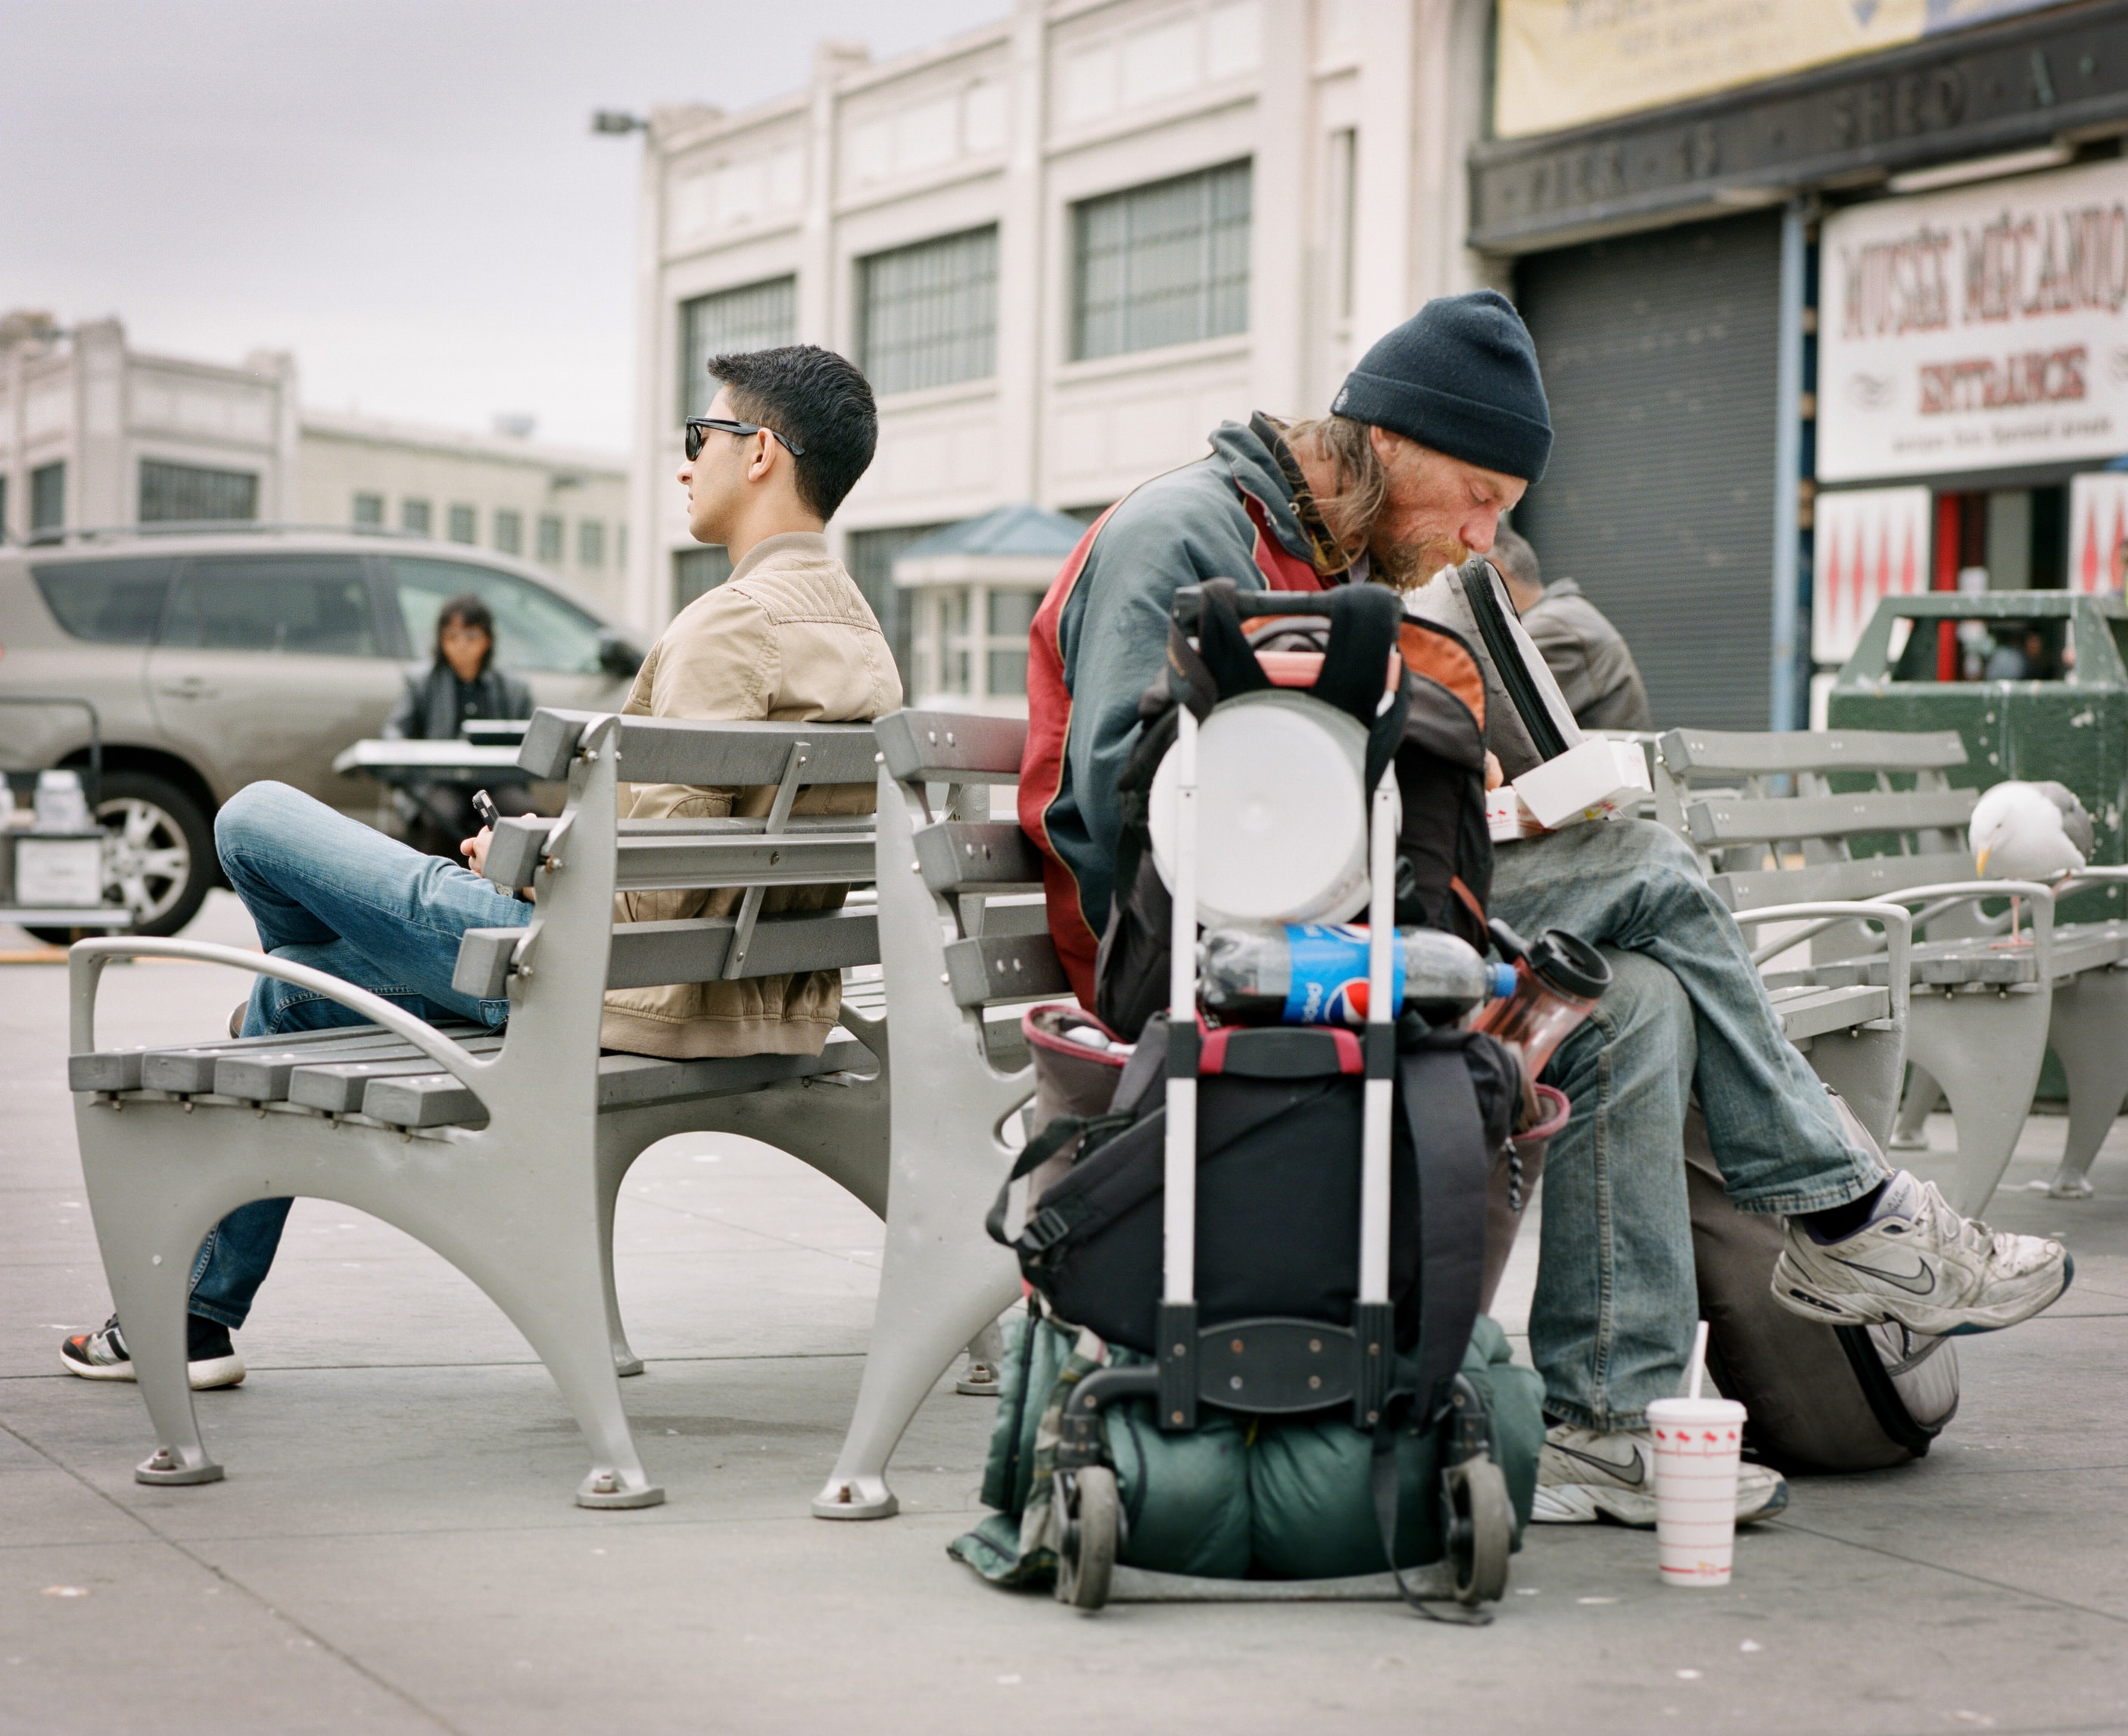
\includegraphics[width=0.5\linewidth]{img/growth/fig1} 

}

\caption{Differences in Wealth. Image Sourced from Unsplash.}\label{fig:growth01}
\end{figure}

Why are some so rich and some others so poor? This question can be posed at the individual level. (See Figure \ref{fig:growth01} above.)

\begin{itemize}
\tightlist
\item
  Why is Elon Musk so wealthy?
\item
  Why are there so many people in the US that are struggling financially and barely surviving?
\end{itemize}

This question can also be answered at the macro or aggregate level. Why are people in some countries so rich and so poor in others? This question has been at the heart of economics ever since \href{https://en.wikipedia.org/wiki/Adam_Smith}{Adam Smith} wrote \emph{An Inquiry into the Nature and Causes of the Wealth of Nations} in 1776. There, you find the statement:

\begin{quote}
``The causes of this improvement, in the productive powers of labor, and the order, according to which its produce is naturally distributed among the different ranks and conditions of men in society, make the subject of the First Book of this Inquiry.''
\end{quote}

This is exactly the question why are some so rich and some so poor.

We can take a long run, and I mean really, really long run, like 3000-year, perspective on this question. The picture below, Figure \ref{fig:growth02}, summarizes the world economic history over the last 3000 years. Not much happened before the year 1750. There were some ripples, some ups and downs, but by and large average incomes were constant. If incomes rose for a while, for whatever reason, the population expanded and the extra number of people ate up the extra income. This is called the Malthusian regime, named after \href{https://en.wikipedia.org/wiki/Thomas_Robert_Malthus}{Thomas Malthus}. The economic history before 1750 depicted below is basically the same in all continents, Europe, south Asia, China, etc. There might have been some differences in the levels of income, but the long run growth rate was zero everywhere.

Then in the 1600s something happened in Europe, first in the Netherlands, then in the UK, then in the US and other European offshoots such as Australia, Canada.

\href{https://en.wikipedia.org/wiki/Paul_Romer}{Paul Romer}, describes how growth slowly took off starting in the 1600 or so when the Netherlands was the wealthiest economy at the time to the 1700 when growth in the UK between 1785 and 1820 was (a measly) 0.5\% annually.

This is the period we now call the Industrial Revolution. This growth of 0.5\% annually does not strike us moderns as a revolution. But we must remember that before that period, there was no growth at all. Nada. Zero. Zilch! Growth was zero. If you go from a world of zero growth for millenia to a world of 0.5\% growth for 40 years, surely that is revolutionary. After 40 years, (two generations?), your income has gone up by over 20\%.

From 1820 to 1890 growth in the UK averaged 1.4\% annually. Incomes went up by a factor of 2.6 in that period. Now that is revolutionary\footnote{\url{https://www.nber.org/system/files/working_papers/w3098/w3098.pdf}}.

\begin{figure}

{\centering 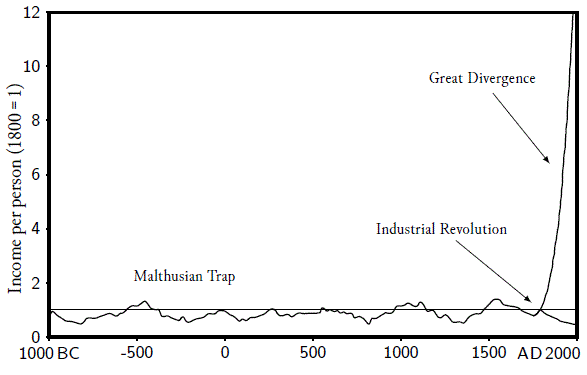
\includegraphics[width=1\linewidth]{img/growth/fig2} 

}

\caption{Image from Gregory Clark, Farewell to Alms: A Brief Economic History of the World (Princeton, N.J.: Princeton University Press, 2007), p. 2.}\label{fig:growth02}
\end{figure}

How do we measure this though? When we talk about there was a 1.4\% growth, what are we talking about? What is growing?

One of the crucial national income accounting concepts is this thing called Gross Domestic Product, or GDP for short.

\hypertarget{gdp}{%
\section{GDP}\label{gdp}}

Gross domestic product (GDP) refers to the value of final goods and services produced in a country within a particular period, usually a year.

While GDP is a great tool to check how a country is doing, it is not an ``end all, be all'' measure of the quality of life. It is but one measure of the quality of life. It measures how many resources you have to buy stuff. It does not measure literacy, longevity, environmental quality and other measures of the quality of life we might care about. It also does not measure how the resources within the country are distributed.

When making comparisons of GDP across countries we need to make adjustments for country size. It will not be a surprise to anyone that the US has higher GDP than Norway. After all, the US has about 60 times as many people as Norway. So, when we adjust for population size by dividing each country's GDP by the number of people, we get for the year 2019, for example.

So, Norwegian GDP per person is about 15\% higher than in USA. That means that the average person in Norway has a purchasing power that is 15\% higher than the average person in the US.

\begin{longtable}[]{@{}cc@{}}
\toprule\noalign{}
Country & Per Capita GDP (in USD) \\
\midrule\noalign{}
\endhead
\bottomrule\noalign{}
\endlastfoot
United States & 65,000 \\
Norway & 75,000 \\
\end{longtable}

When we divide by, or normalize, by population size we are asking the question: How much stuff is available for consumption per person. This is an opulence type question. However when we adjust for country size by dividing GDP, not by the population, but by the number of workers, we are asking the question: How much stuff can each worker produce? This is productivity question. Both questions are certainly valid questions. What kind of data we collect will typically depend on the question we are after.

When making comparisons of GDP, total or per person, it is important that this is not done using the exchange rate of the two currencies used in the two countries. Exchange rates often fluctuate wildly from month to month, week to week, day to day, without really impacting the purchasing power for the typical residents of the countries. These comparisons must be made at what is called ``purchasing power parity'' to be meaningful.

When making comparisons of GDP, total or per capita, for a country over time, it is important to adjust for inflation. Inflation here means persistent changes in the price level. This is more important when comparisons are made over longer time spans rather than comparing GDP for two adjacent years, say comparing US GDP in 2020 to GDP in 1975. A gallon on gasoline at that time cost 57 cents.

\hypertarget{basic-notation}{%
\section{Basic Notation}\label{basic-notation}}

Gross domestic product refers to production. Production requires inputs. In most economic models we will treat GDP as an output and we will assume for starters that there are two inputs, which we will call labor and capital. As a matter of notation, we will let

\[ \text{Y} = \text{GDP} \newline 
\text{N} = \text{the amount of labor used} \newline
\text{K} = \text{the amount of capital used} \]

We can think of the amount of labor being measured either in the total number of workers employed or by the total number of hours worked by all workers in the economy. Capital is the collection of durable inputs used in production. Examples would be the robots on an assembly line, the trucks that bring lettuce from Imperial Valley to Indiana, the computers used for design, the shovels used in construction, etc.

In short we have inputs going in and GDP coming out. But how are the inputs transformed into output? We will refer to this as the production function, F. That is we can write the production function as

\[Y = F(K,N)\]

where F stands for any function which transforms our inputs into outputs. In most applications the function F will have particular properties that are appropriate for the given application.

The production function at the level of an individual firm is an engineering description of the production process. There is very little, if any, economics here. If you are running a barbershop, you need barbers and scissors, to produce haircuts. If you are running an oil refinery you need chemical engineers and crude oil and a few other things to produce gasoline. To produce an iPhone you need rare earth minerals, cobalt and such. No cobalt, no iPhone.

At the level of an entire economy the production function is simply a relationship between the major inputs, things like capital and labor. Sometimes, (this depends on the application, the question at hand), we include raw materials, cobalt?, or energy.

A few things should be clear.

\begin{itemize}
\tightlist
\item
  With the same number of workers if we use more capital, we will get more output. In ``math speak'' that is: The function F is increasing in K (capital), holding N (labor) constant.\\
\item
  The same is true for labor. Holding the amount of capital fixed, the more labor we employ, the more output we get. For a fixed level of K, the function F is increasing in N.
\end{itemize}

\hypertarget{measuring-economic-growth}{%
\section{Measuring economic growth:}\label{measuring-economic-growth}}

We let \(y_t\) denote real per capita GDP in period t. For all time periods t. Then \(y_{t+1}\) is GDP, real and per capita, for period t+1. We let gt denote the growth rate of real per capita GDP. Then we can define the growth of real per capita GDP from period t to period t+1 to be

\[g_t = \frac{y_{t+1} - y_t}{y_t}\]

We can calculate this growth rate for GDP for quarterly data, for annual data or at any frequency where data is available. What frequency we use depends on the particular question we have in mind. If we use quarterly or annual frequencies, we are most likely interested in business cycle questions. For questions of long run growth, we might take calculate growth rates over decades or even longer periods.

\hypertarget{a-thought-experiment}{%
\subsection{A thought experiment}\label{a-thought-experiment}}

This thought experiment goes back to Robert Lucas, Nobel Laureate of the University of Chicago\footnote{\url{https://en.wikipedia.org/wiki/Robert_Lucas_Jr}}. from the 1980s. This experiment shows the power of exponential growth.

\begin{longtable}[]{@{}
  >{\centering\arraybackslash}p{(\columnwidth - 6\tabcolsep) * \real{0.2500}}
  >{\centering\arraybackslash}p{(\columnwidth - 6\tabcolsep) * \real{0.2500}}
  >{\centering\arraybackslash}p{(\columnwidth - 6\tabcolsep) * \real{0.2500}}
  >{\centering\arraybackslash}p{(\columnwidth - 6\tabcolsep) * \real{0.2500}}@{}}
\toprule\noalign{}
\begin{minipage}[b]{\linewidth}\centering
Country
\end{minipage} & \begin{minipage}[b]{\linewidth}\centering
Annual growth rate
\end{minipage} & \begin{minipage}[b]{\linewidth}\centering
Doubling time
\end{minipage} & \begin{minipage}[b]{\linewidth}\centering
Income of grandchild/income of grandparent (in 1960-1985)
\end{minipage} \\
\midrule\noalign{}
\endhead
\bottomrule\noalign{}
\endlastfoot
South Korea & 7\% & 10 years & 32 \\
India & 1.5 \% & 50 years & 2 \\
\end{longtable}

This thought experiment is based on true data. The two numbers in the first column are the actual growth rates for these countries in that period. A South Korean grandchild will be richer than the grandparent by a factor of 32! This is assuming that a generation comes every 25 years, which is an eminently reasonable assumption. A factor of 32 is huge.

Remember this is per capita and it is already adjusted for inflation.\\
If we assume that India and South Korea had he same initial starting conditions in 1960, then after 50 years, the typical South Korean will be 16 times as well off as the typical person in India. That is a stunning difference in purchasing power.

To convince yourself of the enormous difference in the quality of life associated with such large growth rates of 7\% or so, google images of Seoul in 1955 and in 2015. What a difference, like night and day! (See Figure 3.)

Figure 3 What a difference economic growth can make

\hypertarget{the-rule-of-70}{%
\section{The Rule of 70!}\label{the-rule-of-70}}

The Rule of 70 is a convenient way to get an idea of how fast exponential growth can be. It allows us to calculate doubling times, if we know the growth rates.

\begin{itemize}
\tightlist
\item
  How long will it take for GDP to double if the average annual growth rates in x\%?
\item
  How long will it take for my \$1,000 investment to double if the interest rate is y\%?
\item
  How long will it take for Covid-19 infections to double if R0 , the average infection rate is 2.3?
\end{itemize}

The power of exponential growth is often underappreciated.

So here is the rule:

Doubling time = 70/g

where g is the growth rate.

Examples:

\begin{enumerate}
\def\labelenumi{\arabic{enumi}.}
\item
  If the growth rate is 3.5\%. then it will take 20 years for income to double.
\item
  The economy in China started to grow like gangbusters around 1990. After 1990 their growth rate has averaged about 7\% annually. At that rate incomes will double every 10 years. In 2020 Chinese per capita GDP was about \$10,000. Using the rule of 70 we can infer that Chinese GDP per person was:
  \$5,000 in 2010
  \$2,500 in 2000
  \$1,250 in 1990 (That is \$3.40 per day.)
\item
  In the US in 2020 GDP per capita is \$65,000. Over the past 120 years the US growth rate has averaged 1.8 \% annually. Under this growth rate it takes about 40 years for incomes to double. Then, if that continues, we can estimate future income levels in the US to be:
  \$130,000 in 2060
  \$260,000 in 2100
  Imagine that potential!!!
\item
  We can use the data from example 3 to go backwards in history. We can calculate incomes going back in steps of 40 years to get
  \$32,000 in 1980
  \$16,000 in 1940
  \$8,000 in 1900
  \$4,000 in 1860
  Of course, all these exercises work well if the growth rate remains constant at the indicated level. And we have to keep in mind that these are long run projections, approximations and that there can be deviations due to business cycles or other more short- term events\footnote{\url{https://en.wikipedia.org/wiki/Rule_of_72}}
\end{enumerate}

\hypertarget{the-solow-growth-model}{%
\section{The Solow Growth Model}\label{the-solow-growth-model}}

We will begin with a workhorse model that can provide some, but not all, answers. No model will ever provide all answers. In the model, named after Robert Solow, we will first trace out the evolution or growth of the capital stock.

\begin{center}\rule{0.5\linewidth}{0.5pt}\end{center}

A student once said that the Slow model was confusing. I assume it is less confusing than the fast model, so we have made these notes even slower.

\begin{center}\rule{0.5\linewidth}{0.5pt}\end{center}

Learning about the Solow Model can be somewhat challenging, it is not a way most people are used to think. Take the reading slow, reread, stare at it, ask questions. We will get through this chapter together with a deeper understanding of abstract reasoning. It will come to you. Like many things in life, worthwhile things are hard to get. You must fight for it.

\hypertarget{physical-capital-accumulation}{%
\subsection{Physical Capital Accumulation}\label{physical-capital-accumulation}}

Remember that the capital stock is a durable input in production, still like tractors, computers, warehouses, etc. As the input capital increases (declines) we can expect output, GDP, to increase (decline) accordingly. It will be convenient to follow the evolution of the capital stock. Once we figure out what happens with the capital, we can figure out what happens with GDP.

We will follow a small string of mathematical operations. The math may not always be clear to you. Simply return to the meaning of the variables. We try to show both the math and explain in words what the math means. To test your understanding you should be able to put the below equations into words as well.

We start with an accounting identity. \(K_t\) represents the capital stock today, \(K_{t+1}\) represents the capital stock tomorrow. We let \(D_t\) represent the amount of the capital stock that depreciates in that period and we let \(I_t\) represent the amount of new investments made in the period.

If this is a bit abstract think of a trucking company that owns 1000 trucks. That is their capital stock at the beginning of the year 2020. In that year, 20 trucks are retired and go to the truck graveyard. That would leave the company with 980 trucks. But the company buys 30 new trucks, so at the end of the year the company has 1010 trucks.

The other analogy we can use is water in a pond. During the day water evaporates and diminishes the amount of water in the lake. That is depreciation. But at the same time, water enters the pond as well, through runoff from the nearby area and rain that may have ocurred that day. That is investment.

We call depreciation and investment flow variables. They are like water flowing in and out of the pond. We call the amount of capital a stock variable. It is like the total amount of water in the pond.

Our first equation just says: The amount of capital tomorrow is the amount of capital today minus the amount that depreciates plus the amount that is invested. This is an identity.

\[K_{t+1}=K_t-D_t+I_t\]

This is the same thing as our pond example. Tomorrow's amount of water, will just be today's water, plus any that has flowed in, minus any that has evaporated.

To get to the second equation we make the assumption that depreciation is always a constant fraction of the total amount of capital. This is an assumption, that is not necessarily true. In some years there might be more accidents that destroy trucks than in others. There is a certain amount of randomness involved. Here we abstract from this randomness and assume constant depreciation. We call the fraction of the capital stock that depreciates \(\delta\). Of course, \(\delta\) is always between zero and one.

\[=K_t- \delta K_t+I_t\]

To get to the third equation we just use a bit of algebra. We recognize that the first two terms on the right side of the equation contain a common term \(K_t\). So, we factor it out to get the next line.

\[=(1-\delta) K_t+I_t\]

The next step is more substantial, much more substantial. Here we assume that all investment is financed by current domestic savings:

\[I_t=S_t\]

That is, the economy is closed. All investment in the domestic economy comes from domestic savings. The Japanese or the Chinese cannot invest on the US economy. We know that there is typically foreign investment in all economies. Here we rule this out. By assumption.

The first very basic national income accounting identity states:

\[c + i = y\]

where c is consumption, i is investment and y is GDP. This little identity says: Stuff is produced, and you can either eat it, c, or save and invest it, i.

All of this gets us to:

\[=(1-\delta)K_t+S_t\]

\(S_t\) is total savings in the economy in period t. Savings is that part of output that is not consumed.

We can then think that savings can be expressed as some fraction of GDP. That is if GDP is \$ 1,000 and savings was \$ 200, then savings in this case is \(0.2 \times GDP\)

Let's use s (lower case) to denote the savings rate in the economy. In the term \(sY_t\) we look at what is the fraction of total income in the economy that is actually saved. Then as we showed above, \(S_t=sY_t\).

\[K_{t+1}=(1-\delta) K_t+sY_t\]

As noted way back in our Basic Notation section, \(Y_t\) denotes output, or GDP in period t. That output is produced with inputs, capital \(K_t\) and labor input \(N_t\) according to the production function \(F\).

\hypertarget{production-function}{%
\subsection{Production Function}\label{production-function}}

For our basic Solow Growth Model, we assume the production function has the following general properties:

\begin{itemize}
\tightlist
\item
  For a fixed amount of labor, the output is increasing in the amount of capital used, but at a decreasing rate.
\item
  For a fixed amount of capital, the output is increasing in the amount of labor, but at a decreasing rate.
\item
  In ``math speak'' the production function is assumed to be concave.
\item
  In ``econ speak'', we say that the production function exhibits diminishing returns to each input.
\end{itemize}

So, we have in the equation below that output, GDP, is produced with two inputs, capital and labor, according to the production function F. The term \(A_t\) below denotes technological progress. (More on that later!)

\[=(1-δ) K_t+s[A_t F (K_t,N_t)]\]

In the next step we simply assume, for now, that the level of technology stats constant. The time subscript on A has disappeared. So, it does not change over time. This is an assumption that we are making, for now. We will address the question of technological progress later.

\[=(1-δ) K_t+s[A F (K_t,N_t)]\]

In the next step, we simply consider one specific example.

\[=(1-δ) K_t+s A K_t^\alpha N_t^{(1-\alpha)}\]

In that example the parameter \(\alpha\) is any number strictly between zero and one. If \(\alpha\) is large, then capital is very important in production, relative to labor. If \(\alpha\) is small, then labor is more important in production. The appropriate value of \(\alpha\) will depend on the context. In poor countries, agriculture is very labor intensive, low \(\alpha\). In the US, agriculture is very capital intensive, high \(\alpha\).

One more assumption: The population is assumed to be constant. So we can drop the subscript t in the above expression for \(N\).

\hypertarget{in-per-capita-terms}{%
\subsection{In Per Capita Terms}\label{in-per-capita-terms}}

In what we have done so far, we have let all variables be upper cases. Upper cases in this model will always denote totals. Upper case K denotes total capital stock, upper case Y denotes total output, upper case N denotes total employment.

We want to be able to express all or variables in per capita terms. Why?

\begin{itemize}
\tightlist
\item
  We want to be able to make statements about the income growth of the average or typical person and we want to get away from comparing apples, large countries like USA, China to oranges, small countries like Norway or Switzerland.
\item
  We want to be able to compare average income of residents in any country, regardless of country size.
\end{itemize}

That is why we normalize everything from now by N, the size of the country and will express everything in per capita terms. We will let lower cases represent per capita terms. For example, \(k_t\) will be the per person/capita capital stock in period t. Similarly for the other variables.

Then, dividing both sides of the equation by N, the constant population we get
\[\frac{K_{t+1}}{N}=(1-\delta)\frac{K_t}{N}+sA(\frac{K_t}{N})^\alpha\]

Let \(k_t=\frac{K_t}{N_t} = \frac{K_t}{N}\) for all t.

Then we can write the above equation as:

\[k_{t+1}=(1-\delta) k_t+s A k_t^α\]

This is the ultimate expression we will be working with. In our model, this equation will encapsulate the entire evolution of the capital stock. And we can calculate the entire sequence of capital stocks from any arbitrary initial starting point for as long as we like. For the US potential starting points might be the years 1565, 1620 or 1776. For Germany two potential starting points could be 1945 or 1990.

How does this work? Suppose we have estimates for the parameters \(\alpha\), \(\delta\), \(s\), and \(A\). If we also have an estimate for the initial capital stock \(k_0\), say for the US in the year 1776, then we can plug all these estimates into the above equation and calculate \(k_1\), the per person capital stock in period 1. Then we take \(k_1\), the value we just calculated and feed it into the equation to calculate \(k_2\). The we insert \(k_2\) into the equation to calculate \(k_3\).
Etc.
Etc.
Etc.
Until the cows come home.

If you are good with spreadsheets or coding, you can try this. Just pick some values for the above parameters and see what happens, how the capital stock grows over time.

There is an alternative way to \textbf{see} how all of this works. Consider Figure \ref{fig:growth04} below. That figure contains the graph of the above equation with kt on the horizontal axis and \(k_{t+1}\) on the vertical axis.
The graph is concave. It must be concave since one part, the first part, is a straight line with slope \((1 - \delta)\) and the other part \(sA(k_t)^\alpha\) is a concave function. So, the sum of the two is also a concave function. This concave function is the one graphed below.

\begin{figure}

{\centering 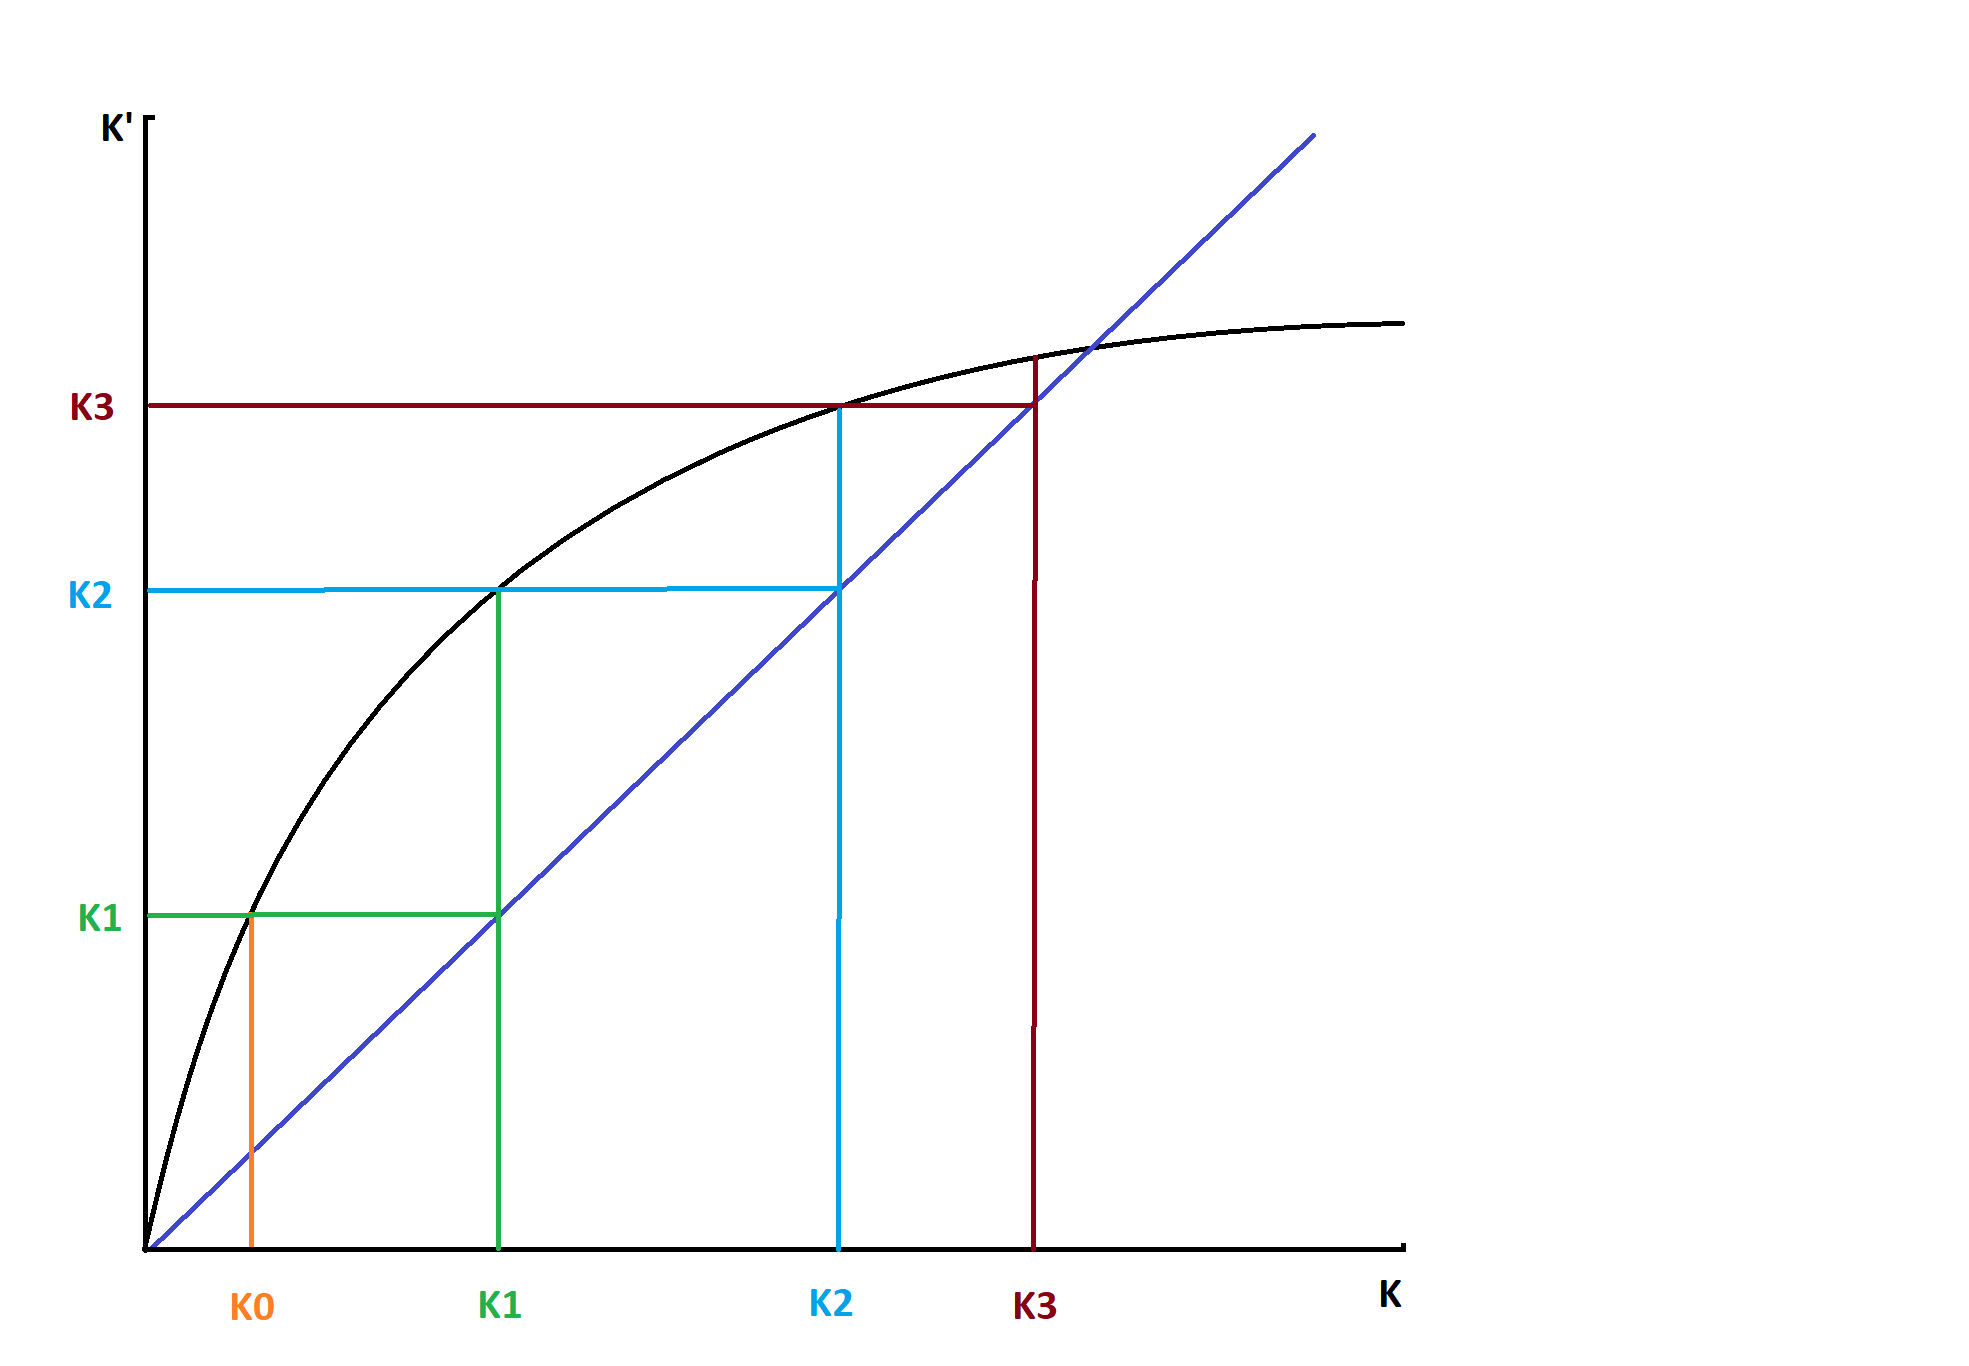
\includegraphics[width=1\linewidth]{img/growth/k3} 

}

\caption{Illustration of Capital Stock Evolution in Solow Growth Model.}\label{fig:growth04}
\end{figure}

We start with \(k_0\) and calculate \(k_1\). We do this by starting at \(k_0\) on the horizontal axis and from there we go up vertically to the graph and then read off \(k_1\) on the vertical axis.

Then we take that value of \(k_1\) on the vertical axis, go over to the 45-degree line and from there go down to the horizontal axis. Now we have \(k_1\) on the horizontal axis. This works because the 45-degree line has a slope of one, which means that the rise is exactly the same as the run. From the origin up to \(k_1\) that is the rise. From the origin over to \(k_1\) that is the run.

We repeat this process: From \(k_1\) go up to the graph, then over to the vertical axis to read of \(k_2\). Bring that value of \(k_2\) from the vertical axis over to the 45-degree line, then go down to the horizontal axis and mark that value of \(k_2\) there.
Repeat.
Etc.
Etc.

Solow Model Capital Accumulation

\hypertarget{predictions}{%
\subsection{Predictions}\label{predictions}}

If we look carefully at the graph above, we see

\textbf{Prediction 1:} The capital stock in an economy increases over time at a decreasing rate. Eventually the capital stock reaches the steady state level \(k_s\).

For any economic variable, the steady state value is that one that stays constant forever once it is reached.
In the graph above we see that the capital stock increases and gets closer and closer to the value ks. Once the capital stock approaches the value where the graph crosses the 45-degree line, there is no escaping. Once you reach that value, you stay there. Forever. That is the steady state level of the capital stock.

\textbf{Prediction 2:} GDP in an economy increases over time at a decreasing rate. Eventually, the GDP reaches a steady state level.

This prediction follows directly from prediction 1. There are two inputs in production, labor and capital. Labor is fixed by assumption. Capital increases over time. Therefore, output, GDP increases over time. And if capital increases at a decreasing rate, then output must, by necessity, increase at a decreasing rate as well. And if capital reaches a steady state, then GDP must reach a steady state as well.

One of the obvious consequences of the second prediction is that eventually output, GDP, will stop growing. There will be no more growth. That is, essentially, just another way of saying that GDP reaches a steady state level.

The reason is simple: Since there are diminishing returns to capital, at a constant savings rate, over time, less and less will be invested in new capital. As less and less gets invested, the capital stock grows less and less and as a consequence, GDP grows less and less.

Eventually, the growth of capital and of output has to come to an end.

\textbf{Prediction 2':} Consider two economies that are equal in all aspects, they have the same parameter values, but they differ in their initial level of capital per person. Then the growth rate of the economy with lower initial capital stock will have higher growth rates and therefore catch up with the richer economy.

This is known as \textbf{The Convergence Hypothesis:} GDP per capita in these economies is predicted to converge. Whether this is true in the data, in which data and to what extent is an interesting question and there is a large literature on this issue.

\hypertarget{solow-model-and-data}{%
\section{Solow Model and Data}\label{solow-model-and-data}}

We will start with data on three large economies, The United States, Japan and China going back to 1950s. We will be utilizing Penn World Tables\footnote{\url{https://www.rug.nl/ggdc/productivity/pwt/?lang=en}} for the data. In the supplemental materials we include the code used to generate the figures.

Comparing the US to Japan between 1960 and 1990 we see what looks like convergence. The difference between the two incomes is getting smaller in that time period. Those of us who followed the news in the 1970s and 80s recall a sense and perhaps a fear that Japan would overcome to US and become the dominant economy in the world. In hindsight this fear was totally unfounded. Even in the 1980s, Japanese income was still much, much lower than US income.

\begin{figure}

{\centering 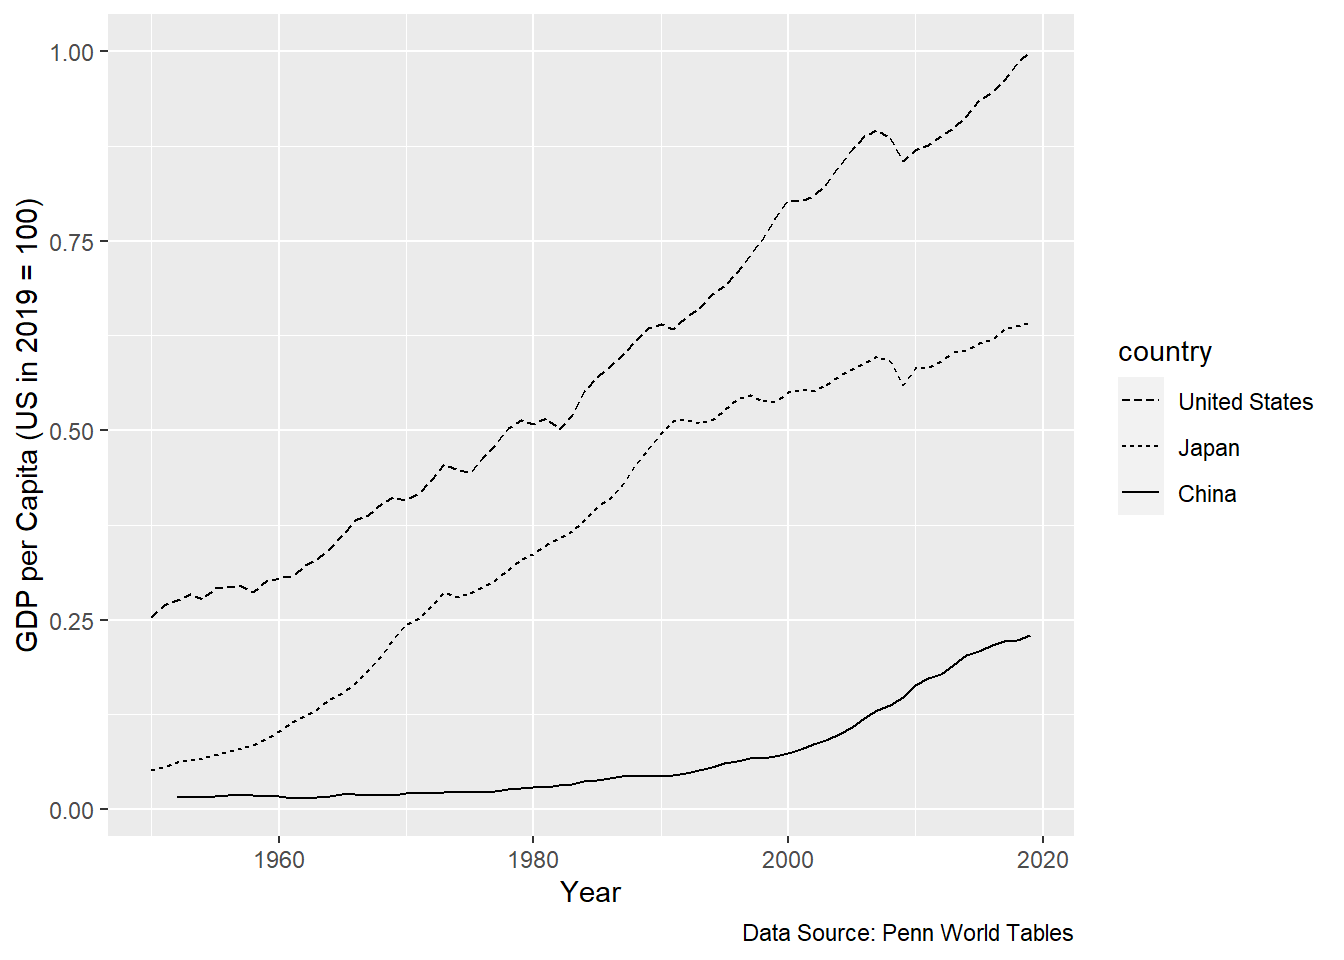
\includegraphics[width=1\linewidth]{introeconfull_files/figure-latex/growth05-1} 

}

\end{figure}

And then something happened in Japan. Growth went AWOL. It disappeared. The US economy kept on growing. The gulf between these two economies widened. Much research has been done on these ``lost decades'' in Japan.

The punchline: Solow like convergence between the US and Japan? Yes, but only initially. After 1990, definitely divergence.

How about the China-US comparison? That comparison only makes sense after 1985 or so. The period before 1980 was plagued by very destructive periods and initiatives such as the Cultural Revolution. It is not surprising that incomes cannot grow under such circumstances. But after 1990, there is a definite convergence between US and Chinese average income. The Chinese economy seems to have grown at unprecedented rates for a long time. There is now, if you follow the news, a fear that the Chinese economy will catch up with the US economy and even overtake it.

But: what the future will bring remains to be seen.

The next figure below, Figure \ref{fig:growth06}, illustrates similar stories, not in terms of levels of income, but in terms of growth rates. The growth rates are 10-year averages so as to filter out business cycle changes. We want to filter out, ignore, the business cycle stuff so we can focus on long run growth.

\begin{figure}

{\centering 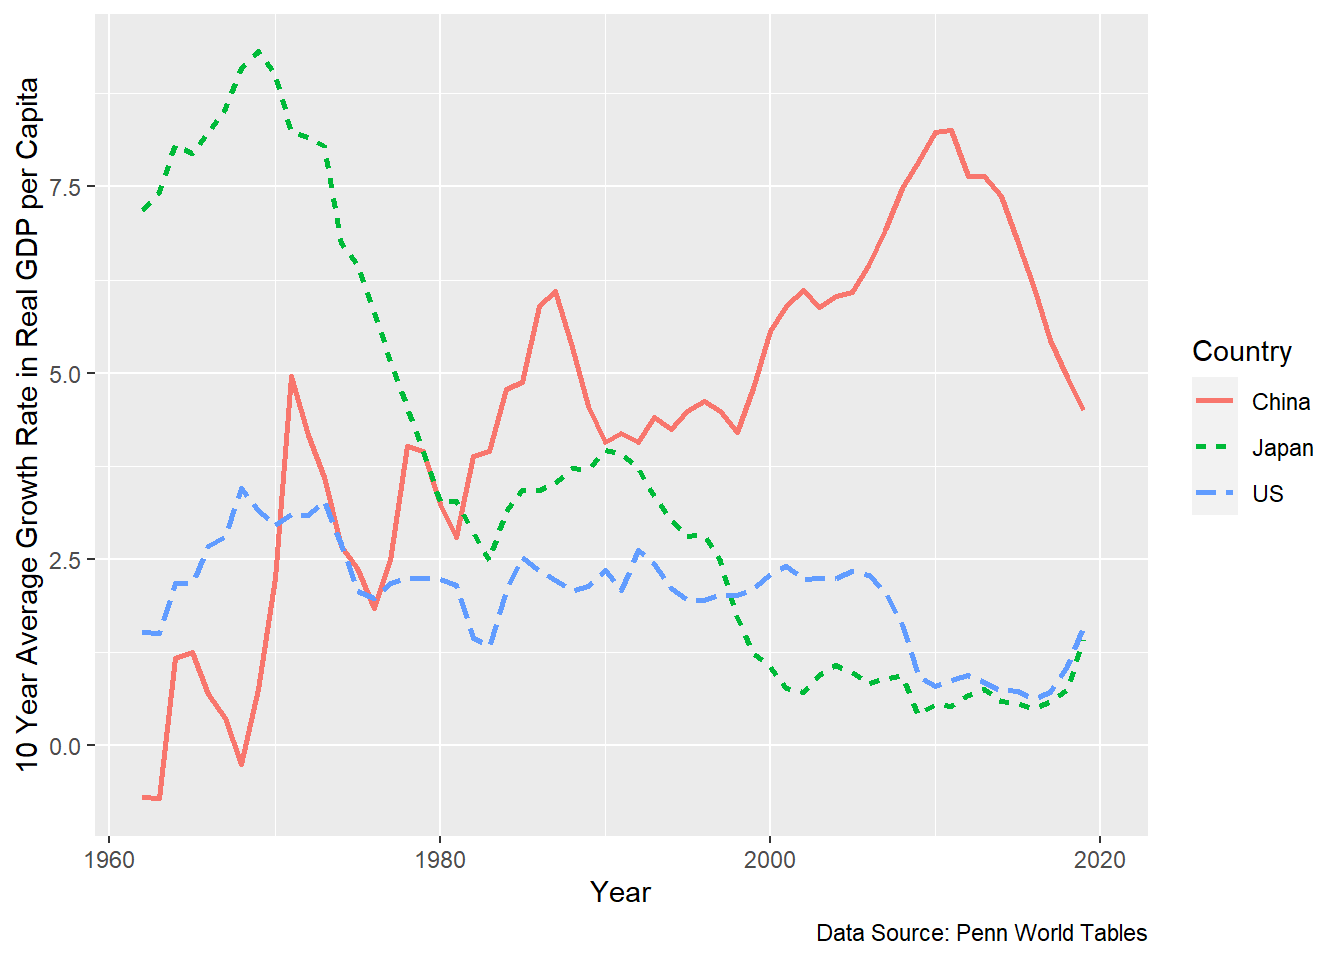
\includegraphics[width=1\linewidth]{introeconfull_files/figure-latex/growth06-1} 

}

\caption{High growth rates in poor countries, low growth rates in rich countries.}\label{fig:growth06}
\end{figure}

For the US the growth rate looks rather constant. There are some ups and downs, but if we tried to fit a straight line into the US observations, that straight line would be rather flat without any clear trend. That is not exactly good news for the Solow model. The Solow model predicts declining growth rates. It is hard to see declining growth rates in these data for the US. But we will have to take a closer look at that later. We will get a better, more detailed view.

The data on Japanese growth rates look more like the Solow prediction. Even though there are wild swings in these growth rate data, the overall trend is clearly downward. Of course, it is a fair and useful question to ask why there was such a large upward spike in the Japanese growth rate in the 1990s, or, perhaps equivalently, such a huge drop in growth rates in the 1970s and 80s. But here we are concentrating on more long-term phenomena. For Japan, the overall trend in the growth rates is clearly down, which is consistent with the Solow model.

How about China? The growth rates for China are rising, inexorably basically starting from the 1960. This seems to be in total contradiction to the Solow model. True. But I think we need to remember that in the 1970s China is emerging out of the Maoist economy with all its shortcomings and distortions. The Solow model was not designed to answer any questions about such transitions. It was designed to answer questions about stable market economies like the US or France or Norway or Japan. So, the failure if the Solow model to be consistent with the data is not really a failure of the model.

The failure of your TV to take you to the Chicago airport is not a failure either. It was not designed to do that.

\hypertarget{post-wwii}{%
\subsection{Post WWII}\label{post-wwii}}

The Solow model does well in the post WWII context. See the Figure below. In 1945 Germany, France, the UK were all more all less bombed out. See the picture of Dresden in 1945 below in Figure \ref{fig:dresden1945}.

\begin{figure}

{\centering 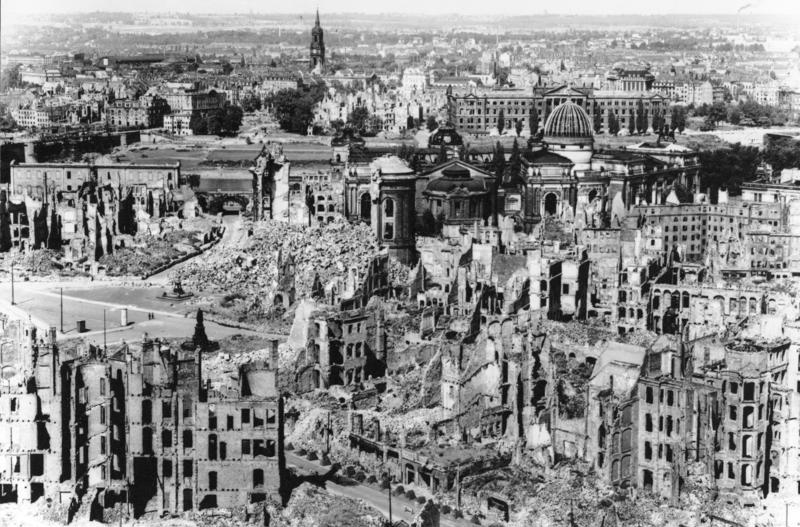
\includegraphics[width=0.5\linewidth]{img/growth/dresden1945} 

}

\caption{Not much capital there. Image Sourced from Wikimedia commons.}\label{fig:dresden1945}
\end{figure}

Without a doubt, the US at the time was the biggest economic power with the highest per capita income. Figure \ref{fig:growth08} below shows: (i) initially the growth rates were high and then they declined over time. (ii) the growth rates in the bombed-out countries were higher than in the US. In Europe, we see large scale convergence of real per capita incomes. This convergence is certainly consistent with the Solow model predictions.

\begin{figure}

{\centering 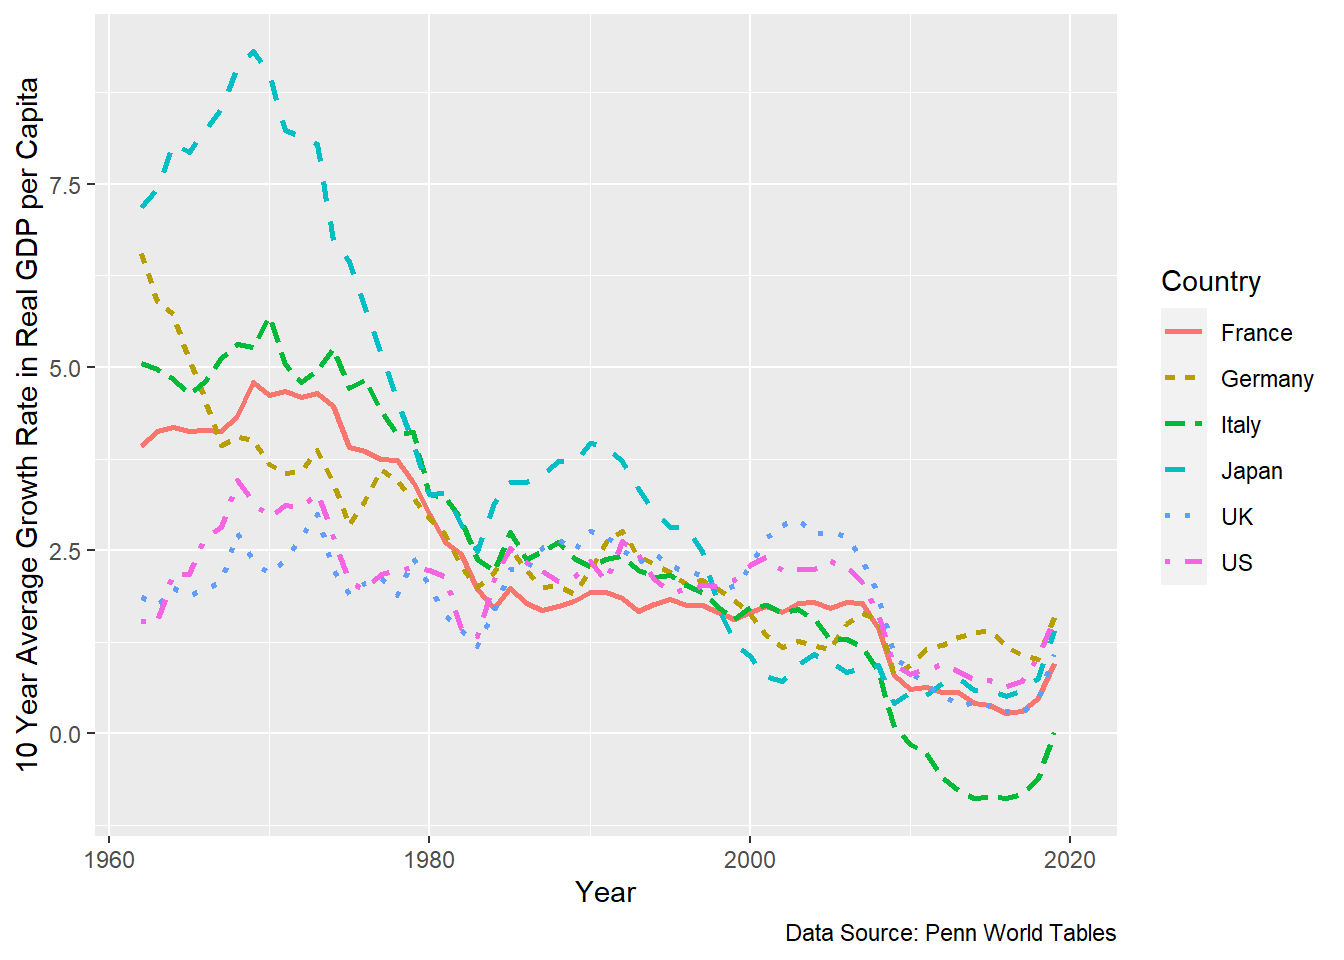
\includegraphics[width=1\linewidth]{introeconfull_files/figure-latex/growth08-1} 

}

\caption{High growth rates in poor countries, low growth rates in rich countries.}\label{fig:growth08}
\end{figure}

If we take a larger sample of countries in Figure \ref{fig:growth09}, we see some evidence of convergence. See below. Countries with higher(lower) levels of income experience lower(higher) growth rates.

\begin{figure}

{\centering 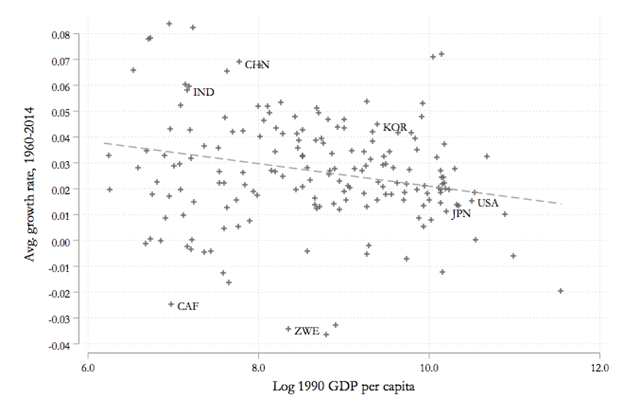
\includegraphics[width=1\linewidth]{img/growth/growth9} 

}

\caption{High growth rates in poor countries, low growth rates in rich countries.}\label{fig:growth09}
\end{figure}

This is for relatively short periods. But if we take a longer historical view, going back 250 years with a larger set of countries, as in Figure \ref{fig:growth10}, we see not just divergence, but DIVERGENCE BIG TIME. This is actually the title of the paper from which the picture below is taken.

\begin{figure}

{\centering 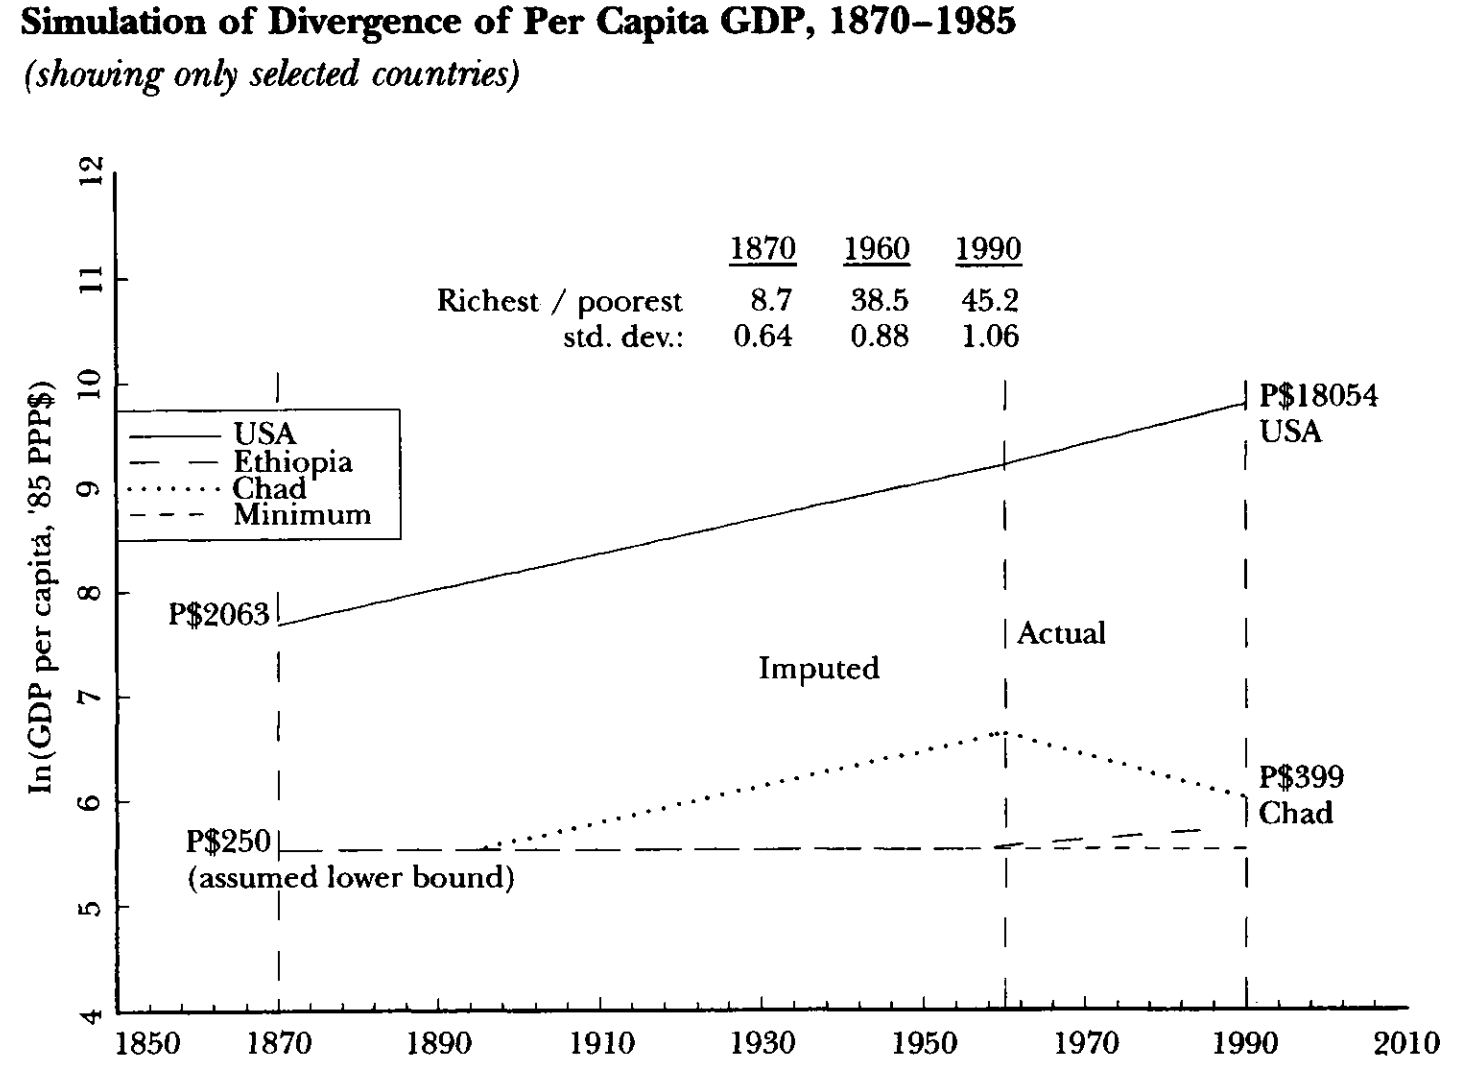
\includegraphics[width=1\linewidth]{img/growth/growth10} 

}

\caption{Massive divergence over the long haul. Source: Pritchett, Divergence Big Time, 1997.}\label{fig:growth10}
\end{figure}

The data in the next two figures, Figure \ref{fig:growth11} and Figure \ref{fig:growth12}, for the US are also not kind to the Solow model. These figures contain data about long run growth in the United States. The figure below shoes the data for real per capita income for the US from 1880 to 1987. The vertical axis is on a logarithmic scale. Using the logarithmic scale makes it easier to see whether growth is constant, increasing or decreasing over time. If you look at the picture you see something that is truly amazing: an almost perfect straight line, with the obvious deviation of the Great Depression and WWII. Apart from that: A perfect straight line.

Absolute constant growth. Over a very long period.

You can even use the data from before the Great Depression, fit a straight line into that subset of the data and use that straight line, the data from before the Great Depression, to ``forecast'' income, real and per capita in 1985. If you did that you would be off by the price of a decent hamburger. In other words: that forecast is right on the money.

This exercise was actually performed by Charles Jones, in the paper mentioned below.

The punchline: In that 100-year time period, the growth rate in the US of real per capita income is constant.

That is a blow to the Solow model.

\begin{figure}

{\centering 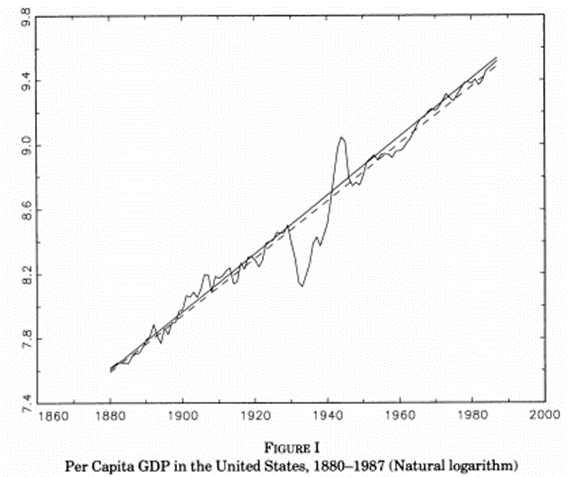
\includegraphics[width=1\linewidth]{img/growth/growth11} 

}

\caption{On a logarithmic scale growth for US looks very constant. Source: Jones, Charles, Time Series Tests of Endogenous Growth Models, QJE 1995.}\label{fig:growth11}
\end{figure}

The next graph makes the same point of constant growth in a different way and points out why the constant growth is really very remarkable.
The bottom panel shows the growth rates of real per capita GDP for the US economy again roughly for a 100-year period. Of course, there are fluctuations, ups and downs. But, if you fit a straight line in the data, it is flat. Totally flat.

The growth rate is constant in this period.

At 1.8\% annually.

This is a number you must remember.

Why is this number important? In just about every election going back to the 1980s, some candidate for President promises to pursue a policy or set of policies that will increase the growth rate to 4\% or higher.

Is this reasonable? Believable?

When these candidates promise 4\% growth or higher, they usually do not talk about per capita growth, so we have to think about that a bit carefully. Over the last 50 years the population growth rate has been less than 1\% per year with a clear downward trend.

If we add the 1.8\% of real per capita growth and at most 1\% of population growth we get 2.8\%. And that is an optimistic upper bound since population growth has been declining. So, any politician who promises 4\% or higher must have something up his/her sleeve that is not revealed in the historical record. Perhaps these candidates know something that we don't know. But then it would be incumbent on them to fill us in on all the details of how such high growth can be accomplished. Otherwise, why would/should we take such claims seriously?

The figure below also points to why the constancy of the growth rate is really an amazing thing. The top panel shows the fraction of GDP collected as income taxes. This fraction increases massively in that period, yet there is no discernible influence of this huge tax increase on the growth rate. Perhaps that is amazing. But there is more.

Over this period education has also increased massively. More and more students are going to college. Average or median years of schooling have increased, almost doubled. This has no discernible impact on the growth rate.

The fraction of women entering the labor force has increased massively over this period. Female labor force participation increased from about 32\% in 1950 to about 60 \% by the year 2000. Again, there seems to be no discernible impact on the growth rate.

Longevity has increased tremendously. Life expectancy has increase from about 46 years in 1900 (that is for males) to about 74 years one hundred years later. This huge increase in life expectancy does not seem to have made any difference to the growth rate.

None of these changes seems to have had much, if any, impact on the economic growth rate. Perhaps that does qualify as being totally remarkable.

\begin{figure}

{\centering 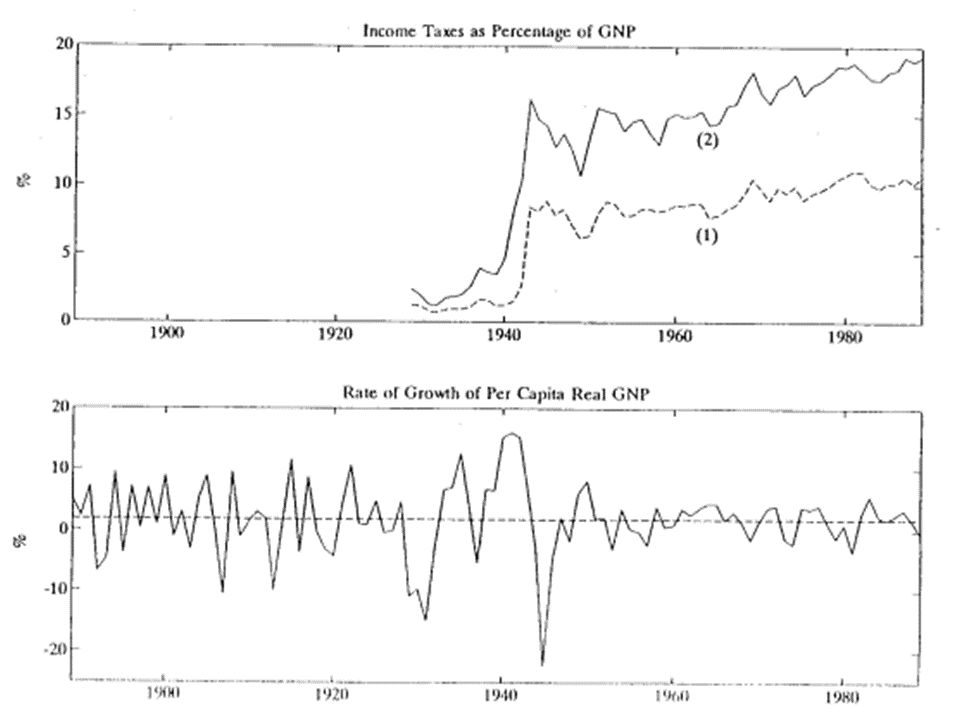
\includegraphics[width=1\linewidth]{img/growth/growth12} 

}

\caption{Constant growth rates. Source: Stokey, N. and S. Rebelo, Growth Effects of Flat Rate Taxes. JPE, 1995.}\label{fig:growth12}
\end{figure}

If we take data for more recent years for the US, we see, if we look carefully in Figure \ref{fig:growth13}, evidence of declining growth.

\begin{figure}

{\centering 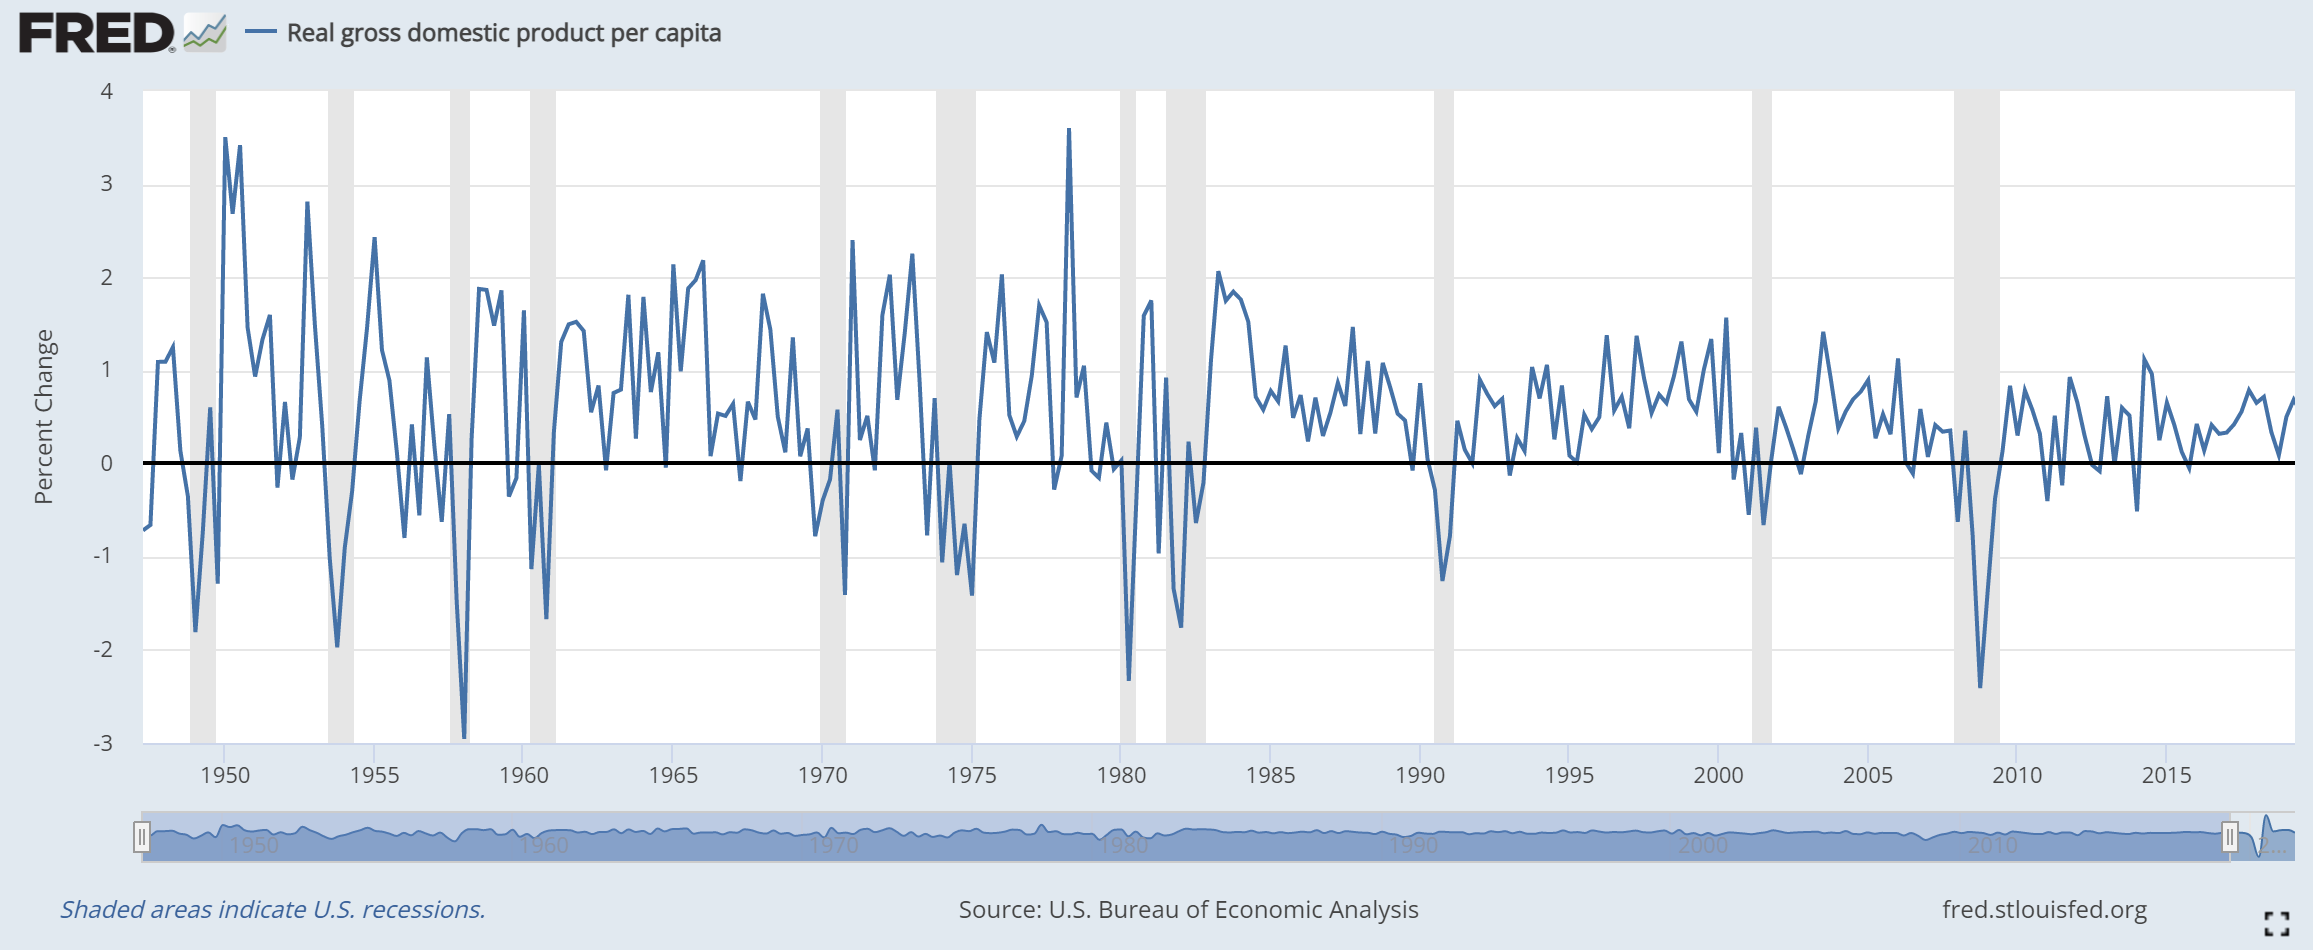
\includegraphics[width=1\linewidth]{img/growth/growth13} 

}

\caption{Evidence of declining growth rates. Source: FRED}\label{fig:growth13}
\end{figure}

We will have to confront the questions:

\begin{itemize}
\tightlist
\item
  Why have growth rates in the US been declining?
\item
  And! Is this decline good or bad?
\end{itemize}

\hypertarget{glossary-of-terms-1}{%
\section{Glossary of Terms}\label{glossary-of-terms-1}}

\textbf{Business Cycle:} fluctuations of economic activity around a long run trend. The periods with activity above trend are called expansions or booms, the periods below trend are referred to as busts or recessions. Usually, these cycles take place over a few years.

\textbf{Convergence Hypothesis:} we might expect income in poorer countries to grow faster than in richer countries. If incomes in poorer countries grow faster than in richer countries, these incomes will come closer and closer and eventually converge.

\textbf{Capital:} an input in production that is durable, that is not used up in production.

\textbf{Depreciation:} the loss of value of capital over time.

\textbf{Diminishing Returns:} the assumption that an extra unit of an input generates more output, but at a diminishing rate. The 200th unit of an input will generate less output than the 30th unit. We will encounter a similar term for consumption.

\textbf{Effective Labor:} refers to the product of raw labor and human capital. It is a measure not of labor time, but of how much labor with a given amount of human capital can produce.

\textbf{Exchange Rate:} the price of one currency, the Euro for example, in terms of another currency, the yen for example.

\textbf{Flow Variables:} economic unit measured over particular units of time.

\textbf{Gross Domestic Product (GDP):} the value of final goods and services produced in a country within a particular time period.

\textbf{Increasing Returns:} when an additional unit of an input generates more output at increasing rates. The 200th unit of an input will generate more output than the 30th unit of that input.

\textbf{Industrial Revolution:} the time period when Western economies switched out of the Malthusian regime and when sustained economic growth started to take off.

\textbf{Input:} any resource that is used to produce an output.

\textbf{Investment:} the addition to the capital stock. Gross investment is the total addition to the capital stock. Net investment refers to investment over and above depreciation.

\textbf{Labor:} input of workers in production. This can be measured by the number of workers hired or by the total number of hours worked.

\textbf{Malthusian Regime:} refers to the time period in economic history when per capita GDP over the long run was roughly constant. Short tun increases in income were followed by increases in fertility, which then soaked up the extra income, this causing a decline in per capita income. This process generated short run fluctuations about a long run trend with zero long run growth.

\textbf{Modern Economic Growth:} the period after the Malthusian regime when economic growth started to take off towards a sustained growth path.

\textbf{Moore's Law:} transistors in an integrated circuit double every two years.

\textbf{National Income Accounting:} government accounting system that keeps track of economic activity.

\textbf{Output:} the goods and/or services produced with the help of inputs.

\textbf{Production Function:} an engineering relationship that indicates the maximum possible output that can be produced with given amounts of the inputs.

\textbf{Raw Labor:} the labor input into production that is measured simply by the total number of workers hired or the total number of hours worked, regardless of their skill or human capital.

\textbf{Rule of 70:} a rule that allows us to calculate the approximate time it takes for the value of variables to double if they grow at an exponential rate. The approximate doubling time is 70 divided by the annual exponential growth rate.

\textbf{Steady State:} An economic variable is said to have reached a steady stated if its value remains constant over time.

\textbf{Stock Variable:} any variable that is measured at a point in time.

\textbf{Total Factor Productivity:} a measure of how much output can be produced with given amounts of the inputs. If output is high (low) with given amounts of the various inputs we say that total factor productivity is high (low).

\hypertarget{practice-questions-1}{%
\section{Practice Questions}\label{practice-questions-1}}

\hypertarget{discussion-1}{%
\subsection{Discussion}\label{discussion-1}}

\begin{enumerate}
\def\labelenumi{\arabic{enumi}.}
\tightlist
\item
  The Bubonic Plague that struck England and much of Europe in the 1300s killed a large part of the population within short periods of time, often within two weeks. It did not discriminate between young and old. Use the Solow growth model to discuss how per capita income for the survivors is impacted by the Plague. Do you expect the income to increase or decrease due to the Plague? Is this change fast or slow?
\item
  After the Plague left England, per capita incomes of the survivors returned roughly to pre-Plague levels. Do you expect that return to have been fast or slow?
\item
  The HIV/AIDS epidemic struck Africa on the 1970s and 1980s with a vengeance. Using the aggregate production function from the beginning of Section 1.9, discuss the different kinds of mechanisms through which HIV/AIDS decreases the level and the growth rate of GDP per capita.
\item
  Haiti is periodically hit by massive earthquakes that often destroy large fraction of the productive capital stock. Graphically illustrate how such a sequence of earthquakes impacts economic growth on the Solow Model.
\item
  In 1981 Chile adopted a system of general and country wide school vouchers. There is much evidence to show that this change in education policy was associated with a drop in reading and in math scores, with higher drop out rates and with higher grade repetition rates. Graphically illustrate how this policy impacted economic growth in Chile. Explain your answer in English prose.
\end{enumerate}

\hypertarget{multiple-choice-1}{%
\subsection{Multiple Choice}\label{multiple-choice-1}}

\begin{enumerate}
\def\labelenumi{\arabic{enumi}.}
\item
  The Solow growth model predicts that

  A. Capital decreases at increasing rates\\
  B. Capital increases at increasing rates\\
  C. Capital grows at a constant rate\\
  D. Capital increases at a decreasing rate
\item
  In the Solow model presented in in class, an increase in the savings rate causes

  A. An increasing in investment\\
  B. An increase in the steady state level of output\\
  C. An increase in the steady state level of capital\\
  D. All of the above
\item
  The Solow model predicts that

  A. Rich countries become poorer\\
  B. Poor countries will surpass rich countries in income\\
  C. Income in poor countries grows at increasing rates\\
  D. Income in poor countries will converge to income in rich countries
\item
  Income in the 5 richest countries relative income in the 5 poorest counties are

  A. Roughly 10\% higher\\
  B. Roughly 100\% higher\\
  C. Higher by a factor of 50\\
  D. Higher by a factor of 12
\item
  Imagine a country where in the year 2000 average income is 2000 Schmuckers, (their currency). The annual growth rate of average real per capita income is 14\%. Then income in that country in the year 2015 in Schmuckers is

  A. 4,000\\
  B. 8,000\\
  C. 16,000\\
  D. 32,000
\item
  In the US in the year 2020 average income is \(\$80\). Incomes have grown by 3.5\% annually. Using the rule of 70, what is average income in the US in 1960 in \$?

  A. 40\\
  B. 20\\
  C. 10\\
  D. 5
\item
  You stick \$1000 into some asset that pays an annual rate of return of 3.5\%. In 20 years, the value of your investment will be in dollars

  A. 1500\\
  B. 2000\\
  C. 2500\\
  D. 2700
\item
  The prediction in the Solow model of GDP growing but at declining growth rates is due to the assumption of

  A. Increasing returns\\
  B. Constant returns\\
  C. Decreasing returns\\
  D. Complementarity between labor and capital
\item
  In the Solow growth model, in increase in the rate of depreciation causes

  A. An increase in the capital stock\\
  B. A decrease in the capital stock\\
  C. The capital stock to stay constant\\
  D. An increase in consumption
\item
  In the US the growth rate of real per capita GDP between 1900 and 2000 was roughly constant at 2 \% per year. This

  A. Is consistent with the predictions of the Solow model\\
  B. Is inconsistent with the predictions of the Solow model\\
  C. Implies that real per capita GDP doubles every 25 years\\
  D. Implies that real per capita GDP doubles every 45 years
\item
  Imagine that in the Solow model the production n function is given by y = Ak, then

  A. The growth rate is constant over time\\
  B. The growth rate is increasing over time\\
  C. The growth rate is decreasing over time\\
  D. The growth rate increases at first and then decreases.
\item
  Which of the following is the best measure of human capital if we want to assess skills of the labor force in a variety of countries?

  A. Average years of schooling\\
  B. Median years of schooling\\
  C. PISA scores in math and science\\
  D. The college graduation rate
\item
  Between 1950 and 1980 real Japanese GDP per capita relative to real US GDP per capita

  A. Increased\\
  B. Decreased\\
  C. Stayed constant\\
  D. Decreased at first and then increased
\item
  Moore's Law

  A. is an example of arithmetic growth\\
  B. is an example of exponential decline\\
  C. is an example of exponential growth\\
  D. does not hold in the data between 1970 and 2000
\item
  Mortality rates from breast cancer in the US fell while

  A. The number of researchers working on cancer treatment was constant\\
  B. The number of clinical trials for cancer treatments was constant\\
  C. The number of scientific publications about cancer was increasing over time\\
  D. The number of scientific publications about cancer was increasing over time
\item
  Since about 1980 the productivity of cancer research has

  A. Increased\\
  B. Decreased\\
  C. Stayed constant\\
  D. Decreased initially and then increased
\item
  The largest share of the growth of real per capita GDP in the US since 1950 can be explained by

  A. The increase in the capital stock per worker\\
  B. The increase in educational attainment\\
  C. Technological progress\\
  D. Increased social security spending
\item
  In the Solow model presented in class an increase in social security payments to the old decreases capital accumulation since it

  A. Decreases tax rates\\
  B. Provides a higher incentive to save\\
  C. Provides a lower incentive to save\\
  D. Provided an incentive to postpone retirement
\item
  Increased subsidies for attending college are expected to

  A. Increase the stock of human capital\\
  B. Increase the stock of physical capital, if human and physical capital are complements\\
  C. Increase GDP if initial college attendance is low\\
  D. All of the above
\item
  Imagine two countries that are equal in all aspects except for one: Country 1 has a high stock of physical capital and country 2 has a low stock of physical capital. Then in this two-country version of the Solow model we would expect

  A. Capital to flow from country 1 to country 2\\
  B. Capital to flow from country 2 to country 1\\
  C. Capital to be more productive on the margin in country 1 than in country 2\\
  D. A and C
\end{enumerate}

\hypertarget{answer-key-1}{%
\subsection{Answer Key}\label{answer-key-1}}

\begin{enumerate}
\def\labelenumi{\arabic{enumi}.}
\tightlist
\item
  D
\item
  D
\item
  D
\item
  C
\item
  C
\item
  C
\item
  B
\item
  C
\item
  B
\item
  B
\item
  A
\item
  C
\item
  A
\item
  C
\item
  D
\item
  B
\item
  C
\item
  C
\item
  D
\item
  A
\end{enumerate}

\hypertarget{growth2}{%
\chapter{Economic Growth II}\label{growth2}}

In this chapter you will learn:

\begin{itemize}
\tightlist
\item
  The basics of human capital accumulation
\item
  The basics of technological progress
\end{itemize}

\hypertarget{human-capital-accumulation}{%
\section{Human capital accumulation}\label{human-capital-accumulation}}

In the Solow model we considered in the previous sections, there was only one factor to be accumulated: physical capital. In this section we will allow for two augmentable factors: physical capital and human capital.

By human capital we simply mean all the marketable skill. In the Solow model the production function is given by
\[y_t=A F(k_t)\]

Recall that when we hold labor constant, then output is basically a function of capital only and the production function exhibits diminishing returns to capital.
We will now generalize the production function to

\[Y_t = A F (K_t, H_tN_t)\]

In this formulation \(N_t\) stands for labor as before. Labor could be measured by the total number of people employed or by the total number of hours worked. \(K_t\) is the total capital stock, \(Y_t\) is output of GDP and \(A\), as before is a measure of technology.

What is new here is \(H_t\), which stands for human capital. What we do here is we multiply \(H_t\) and \(N_t\) together to get

\[H_tN_t\]

We call this product ``effective labor''. We can think of \(N_t\) as hours worked. If we multiply the hours worked \(N_t\) with skill or human capital \(H_t\) we can get a measure of how much can be done or accomplished in the time spent working. We will refer to \(N_t\) as ``raw labor'' and to \(H_tN_t\) as ``effective labor''.

Effective labor varies both across countries and over time. The average Norwegian worker has more human capital and thus more effective labor then the average Nepali worker. Also, the typical American worker now has more human capital than the typical American worker had 100 years ago.

Just like physical capital, human capital can be accumulated; it can grow. It can also depreciate or become obsolete.

There are multiple ways to accumulate human capital.

\begin{itemize}
\tightlist
\item
  Formal schooling
\item
  Learning on the job
\item
  Leaning by doing
\end{itemize}

There is a large literature on each one of these components. Here we will focus on formal schooling, partially because in many countries formal schooling budgets take up large fractions of national income, GDP. In some cases, this is more than 5 or 6 \% of GDP.

One way to measure formal schooling is through expenditures. How much do we spend as a fraction of GDP on formal public education? When answering this question we have to be cognizant of the fact that there is also a significant private expenditure in formal schooling.

The second way to measure formal schooling or education is simply to ask how many years of schooling do students get. Of course, in every country there will be a distribution. Often, we categorize this the different stages of education completed, such as college completion or high school completion.

Figure 14 below shows that education in the US has increased tremendously. The fraction of the labor force that has completed college has increased substantially while the fraction of the labor force that has only finished elementary education or not finished high school has fallen drastically.

\begin{figure}

{\centering 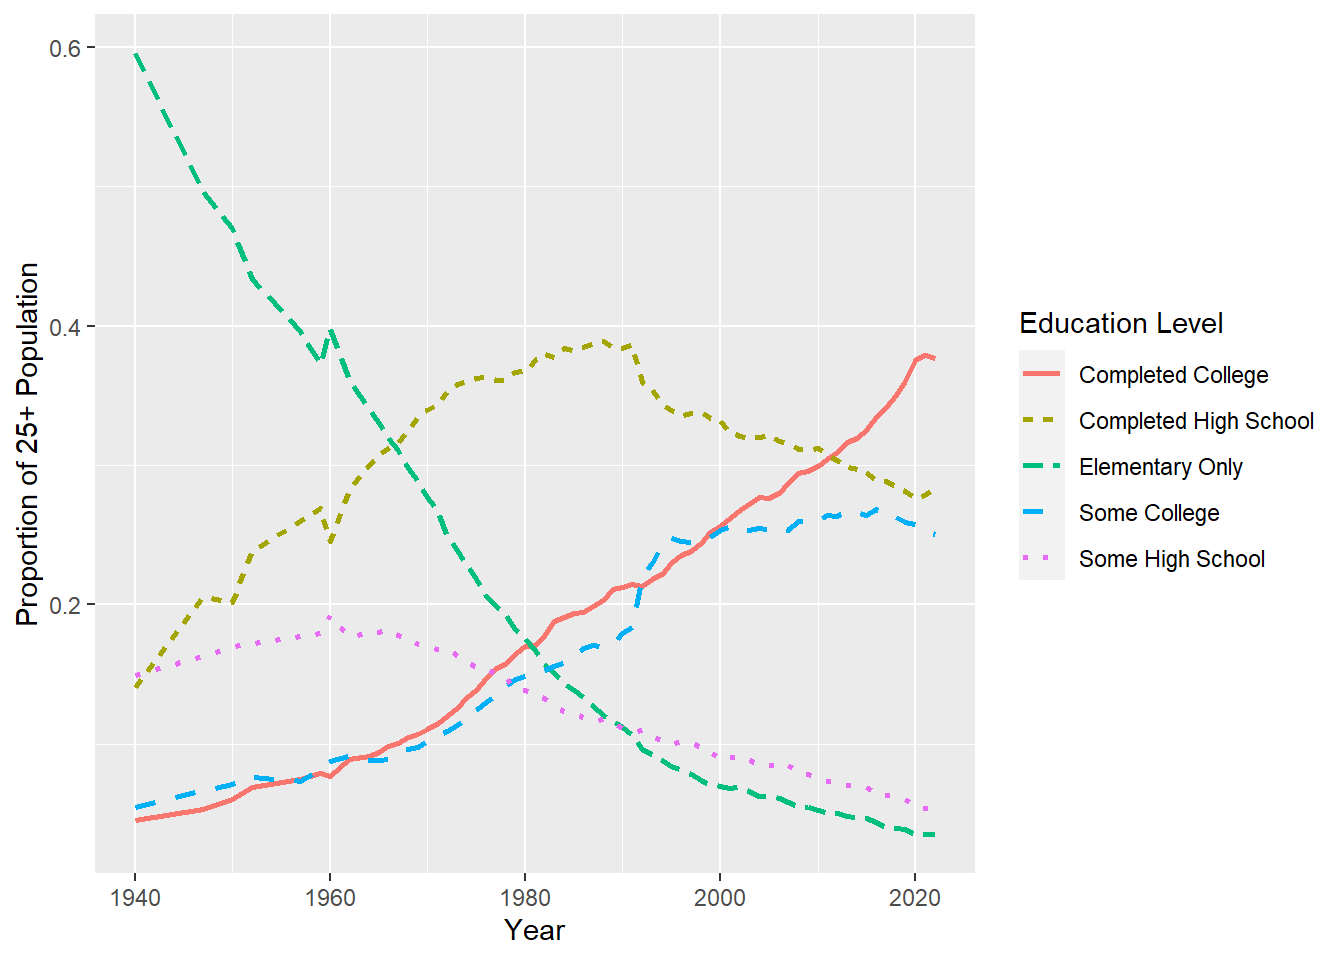
\includegraphics[width=1\linewidth]{introeconfull_files/figure-latex/increasingschooling-1} 

}

\caption{Increasing schooling time. Data Source: US Census Bureau}\label{fig:increasingschooling}
\end{figure}

Most countries have seen similarly large increases in years of schooling. Measured in average or median years or schooling. Or measured in the fraction of the labor force that has completed college.

Beware of measurements!

Measurements should be useful for the purpose at hand.

Measurements should not be too costly.

Both of these are worthwhile considerations.

But, sometimes measurements are taken simply because they are cheap. Please consider the link below. There are reports from central planning in the Soviet Union by plans being fulfilled by a very small number of huge nails or, alternatively, by a huge number of tiny nails. It all depended on the specifications given by the planner to the factory.

See the cartoon below.

\begin{figure}

{\centering 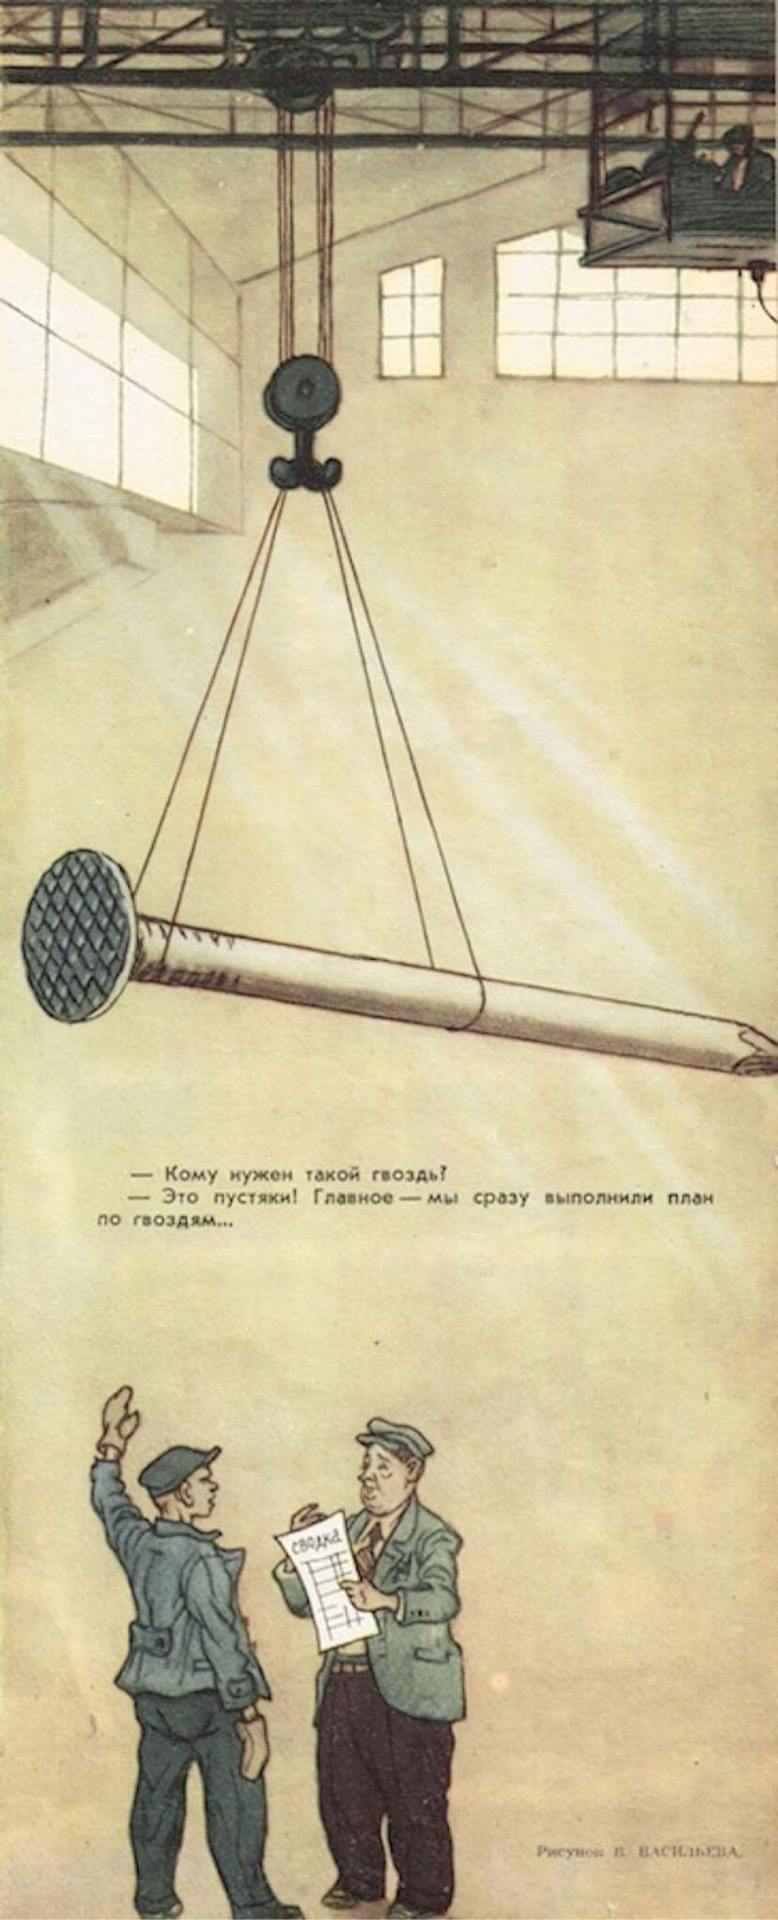
\includegraphics[width=0.5\linewidth]{img/growth2/sovietcartoon} 

}

\caption{Source: Krokodil}\label{fig:sovietcartoon}
\end{figure}

Incentives work!

They work really well.

There is a similar story about shoes in the Soviet Union. People were always lining up for shoes. Always. I mean always. It turns out that the Soviet Union at the time produced hundreds of millions of shoes per year. More shoes than were produced in the US.

The problem: They were just shoes, but not shoes consumers wanted. They were just not comfortable. And forget fashionable.

So the statement above about people standing in line for shoes needs a qualification. People were standing in line not just for shoes, not just for any pair of shoes. They were standing in line for comfortable shoes, for durable shoes, for practical shoes, for shoes that fit their needs.

Why am I telling you nail and shoe stories?

In education there is the risk, that we are looking at numbers, data, measurement in a way that is very similar to the way data were looked at in the nail and shoe stories.

In education we sometimes look at numbers that are easy to collect. And sometimes these numbers are not meaningful. Or at least, it is not clear how meaningful they are.

\begin{itemize}
\tightlist
\item
  Years of schooling.
\item
  The fraction of 18 years olds going to college.
\item
  The number of hours spent studying
\end{itemize}

All these data fall into the category of questionable data. Whether data is questionable ALWAYS depends on a particular purpose: Is that data useful for my particular purpose?

So what could/would be our purpose here? We would hope that education makes people more productive. If education makes people more productive, we would see the effect of education in GDP.

Now, before we take a closer look at the connection between education and GDP, we can use some introspection to think about how useful or how accurate the above three measure can be.

Go back to high school and think of all the students who were you in graduating class. At that point they all had 12 years of schooling. Now consider the difference, if there is any, in the marketable skills among all the graduates in your class? Is that difference small? Is it large? How much do we miss in terms of productivity if for all these students, we just record 12 years of schooling?

Now think of two typical 18 year olds going to college. They are the same in all respects, expect one: Jill attends IU Kokomo; and Jackie attends Princeton. Should both Jackie and Jill be counted equally as attending college? Which one might be more productive in the labor force? How big might such differences in labor productivity be?

John and Jack both are first year students at IU. Both are studying psychology. Both John and Jack report that, outside of class, they spend 20 hours per week studying. Would/should we expect John and Jack to learn equally during those 20 hours. John concentrates on his work and Jack texts with his girlfriend, checks the stock market and pays his bursars bills while doing his homework. Should we count these two sets of 20 hours the same?

Apart from these issues, all of these are measurements of inputs, not of outputs. The outputs are what is actually learned. What are the marketable and other skills? We should care about the outputs, more than the inputs. The outputs are hard to measure, the inputs are easier to measure. So, we will measure the inputs.

Hanushek and Kimko in their paper from 2000: \href{https://www.researchgate.net/profile/Eric-Hanushek/publication/4980899_Schooling_Labor-Force_Quality_and_the_Growth_of_Nations/links/551427960cf283ee0834ac50/Schooling-Labor-Force-Quality-and-the-Growth-of-Nations.pdf}{Schooling, Labor-Force Quality, and the Growth of Nations} make a big effort to get this right. For a bunch of countries, they look at the correlation between years of schooling and economic growth. They do find a positive correlation, exactly what one might expect. But correlation allows for causation in both directions: More years of schooling could imply higher growth. Higher economic growth induces people to get more schooling. So inferring causality from more years of schooling to economic growth is dicey.

There is more. We actually have data on math and science scores of students at the high school level that are comparable across countries. This is a measure of an output, things that students actually learned and know. As an aside, the US performance in these international tests is very mediocre.

If we introduce this measure of student scores in our statistical analysis of schooling and economic growth, the correlation between years of schooling and economic growth goes to zero and the correlation between learning scores and economic growth is positive. And it is large. Very large.

A one standard deviation increase in these test scores is associated with a 1.4\% increase in the growth rate. This is huge. Recall that for the longest time the growth rate of real per capita income in the US has been 1.8\% annually. So, if, somehow magically, or perhaps less magically by prudent choice of education policy, the test scores of US students could be increased by 1.4\% to 3.2\%. That is big. Very big.

Imagine that we start with an income of \$60,000. In one case we have a growth rate of 1.8\% and in the other case we have a growth rate of 3.2\%. Then we have income after 10 years

\[\$60,000 (1.018)^{10} = \$71,718 \]

\[\$60,000 (1.032)^{10} = \$82,214\]

A ten thousand dollar difference is large, by any stretch of the imagination. We could have made this appear even bigger by calculating differences twenty of thirty years out.

There are two more stunning observations that come out of the above paper.

\begin{enumerate}
\def\labelenumi{\arabic{enumi}.}
\tightlist
\item
  Economic growth in that sample of countries is uncorrelated with public expenditures on education.
\item
  The test scores in that sample of countries are uncorrelated with public expenditures on education.
\end{enumerate}

Putting these two things together means that the amount of resources does not matter that much. What matters more is what you do with them.

\hypertarget{more-human-capital}{%
\section{More Human Capital}\label{more-human-capital}}

It is well to consider the correlation between PISA scores and economic growth as done by Hanushek and Kimko, but there is certainly room to do more. Perhaps one can really construct a measure of that H variable that shows up in our production functions, or at least a proxy.

This is done by Egert et al.~(2022)\footnote{\url{https://www.cesifo.org/en/publikationen/2022/working-paper/new-macroeconomic-measure-human-capital-exploiting-pisa-and-piaac}}.

First: The PISA scores measure what 15 years old know. Much of that knowledge might disappear before these youths reach their productive years in the labor force. There is a measure of adult knowledge called the Programme for the International Assessment of Adult Competencies, PIAAC. This measures adult literacy, numeracy and problem-solving skills. As a drawback this is only available for relatively few countries. Egert et al.~show that PISA scores and PIAAC scores are highly correlated. So, they can use the PISA scores in their attempt to construct a measure of human capital.

Second: Then Egert el al.~constructs their measure of human capital for about 80 countries by combining PISA scores and median years of schooling. And there is one more issue. If we look at the US or any other labor force now, we are looking at 20-year-old workers, 65-year-old workers and workers of all ages in between. The 20-year olds were 15 just 5 years ago. The 65 years olds were 15 years of age 50 years ago in 1972. So, we have to average all these PISA scores over all these ages or cohorts. When we do this, the US is sort of in the middle of the pack just above Austria, Hungary, Spain and Italy but below these countries:

France, Slovakia, Belgium, Sweden, Poland, Czech Republic, etc.

The highest countries by this measure are: South Korea, Finland, Japan.

Third: Their constructed measure of human capital is highly correlated with Total Factor Productivity. That is the A in our production functions. This is illustrated in Figure \ref{fig:egertfig5} below.

\begin{figure}

{\centering 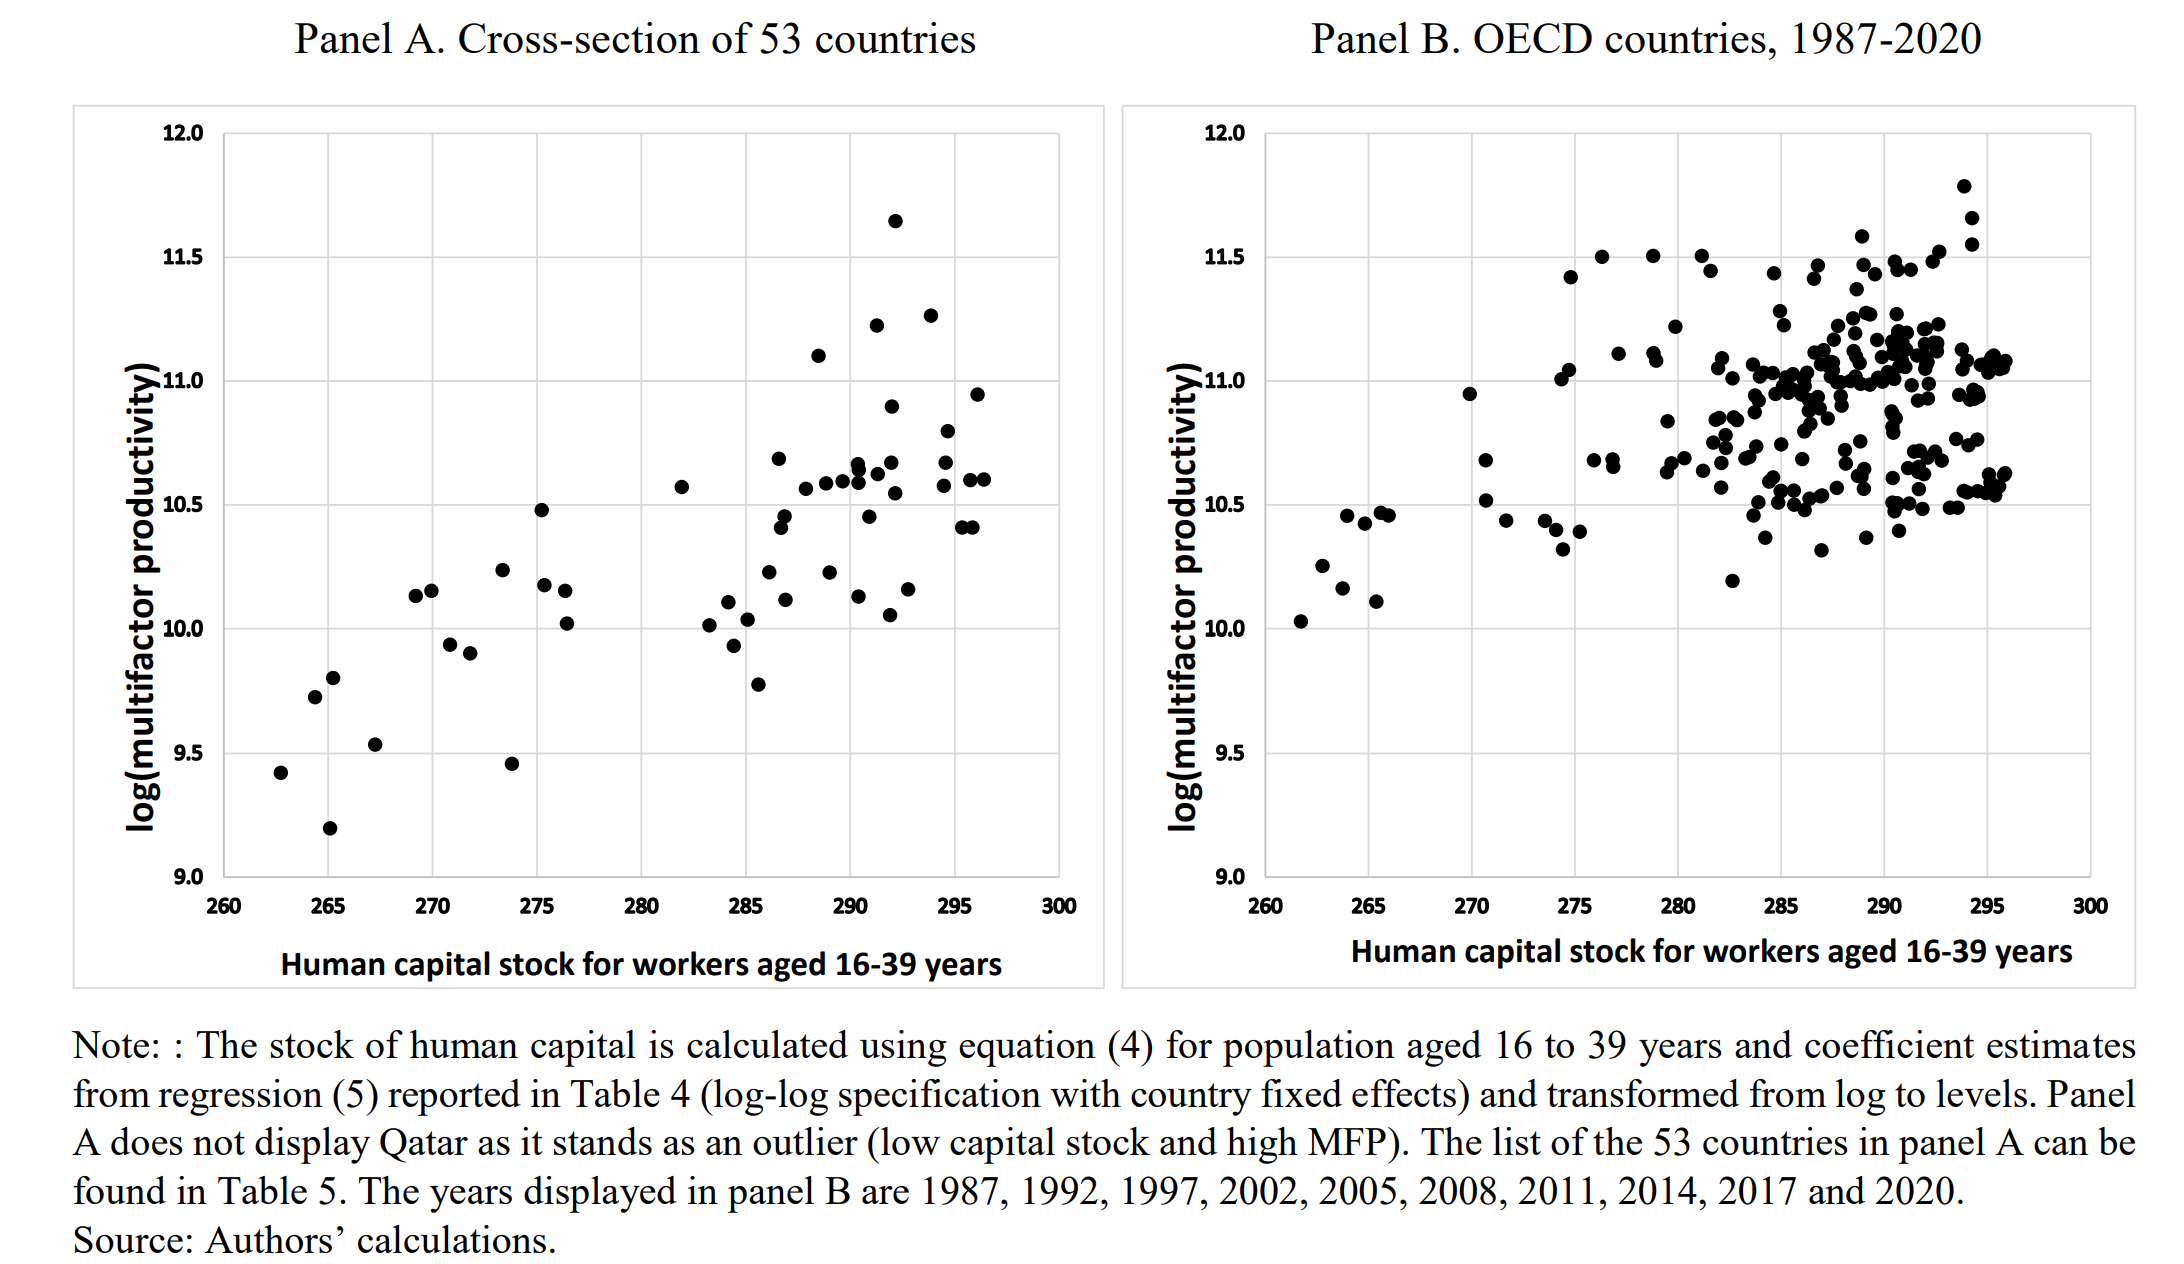
\includegraphics[width=1\linewidth]{img/growth2/egertfig5} 

}

\caption{Taken directly from Egert et al (2022) Figure 5}\label{fig:egertfig5}
\end{figure}

Fourth: Which aspect of human capital, the PISA score or median years of schooling is more important for increases in productivity? It turns out the effect of increasing PISA scores is about twice as big as the effect of increasing median years of schooling.

Fifth: Early childhood intervention

There is a large literature by now on the effects of early childhood intervention. Heckman et al.~(2010) is just one example. So, what is early childhood intervention? Substantial education programs for children at risk and their moms. There is a lot of evidence that the rate of return, the benefit-cost ratio, the bang for the buck is increasing the younger are the students. It is truly very large for the youngest students, three and four year olds. The US is near the bottom of this distribution. See Figure \ref{fig:egertfig7}.

\begin{figure}

{\centering 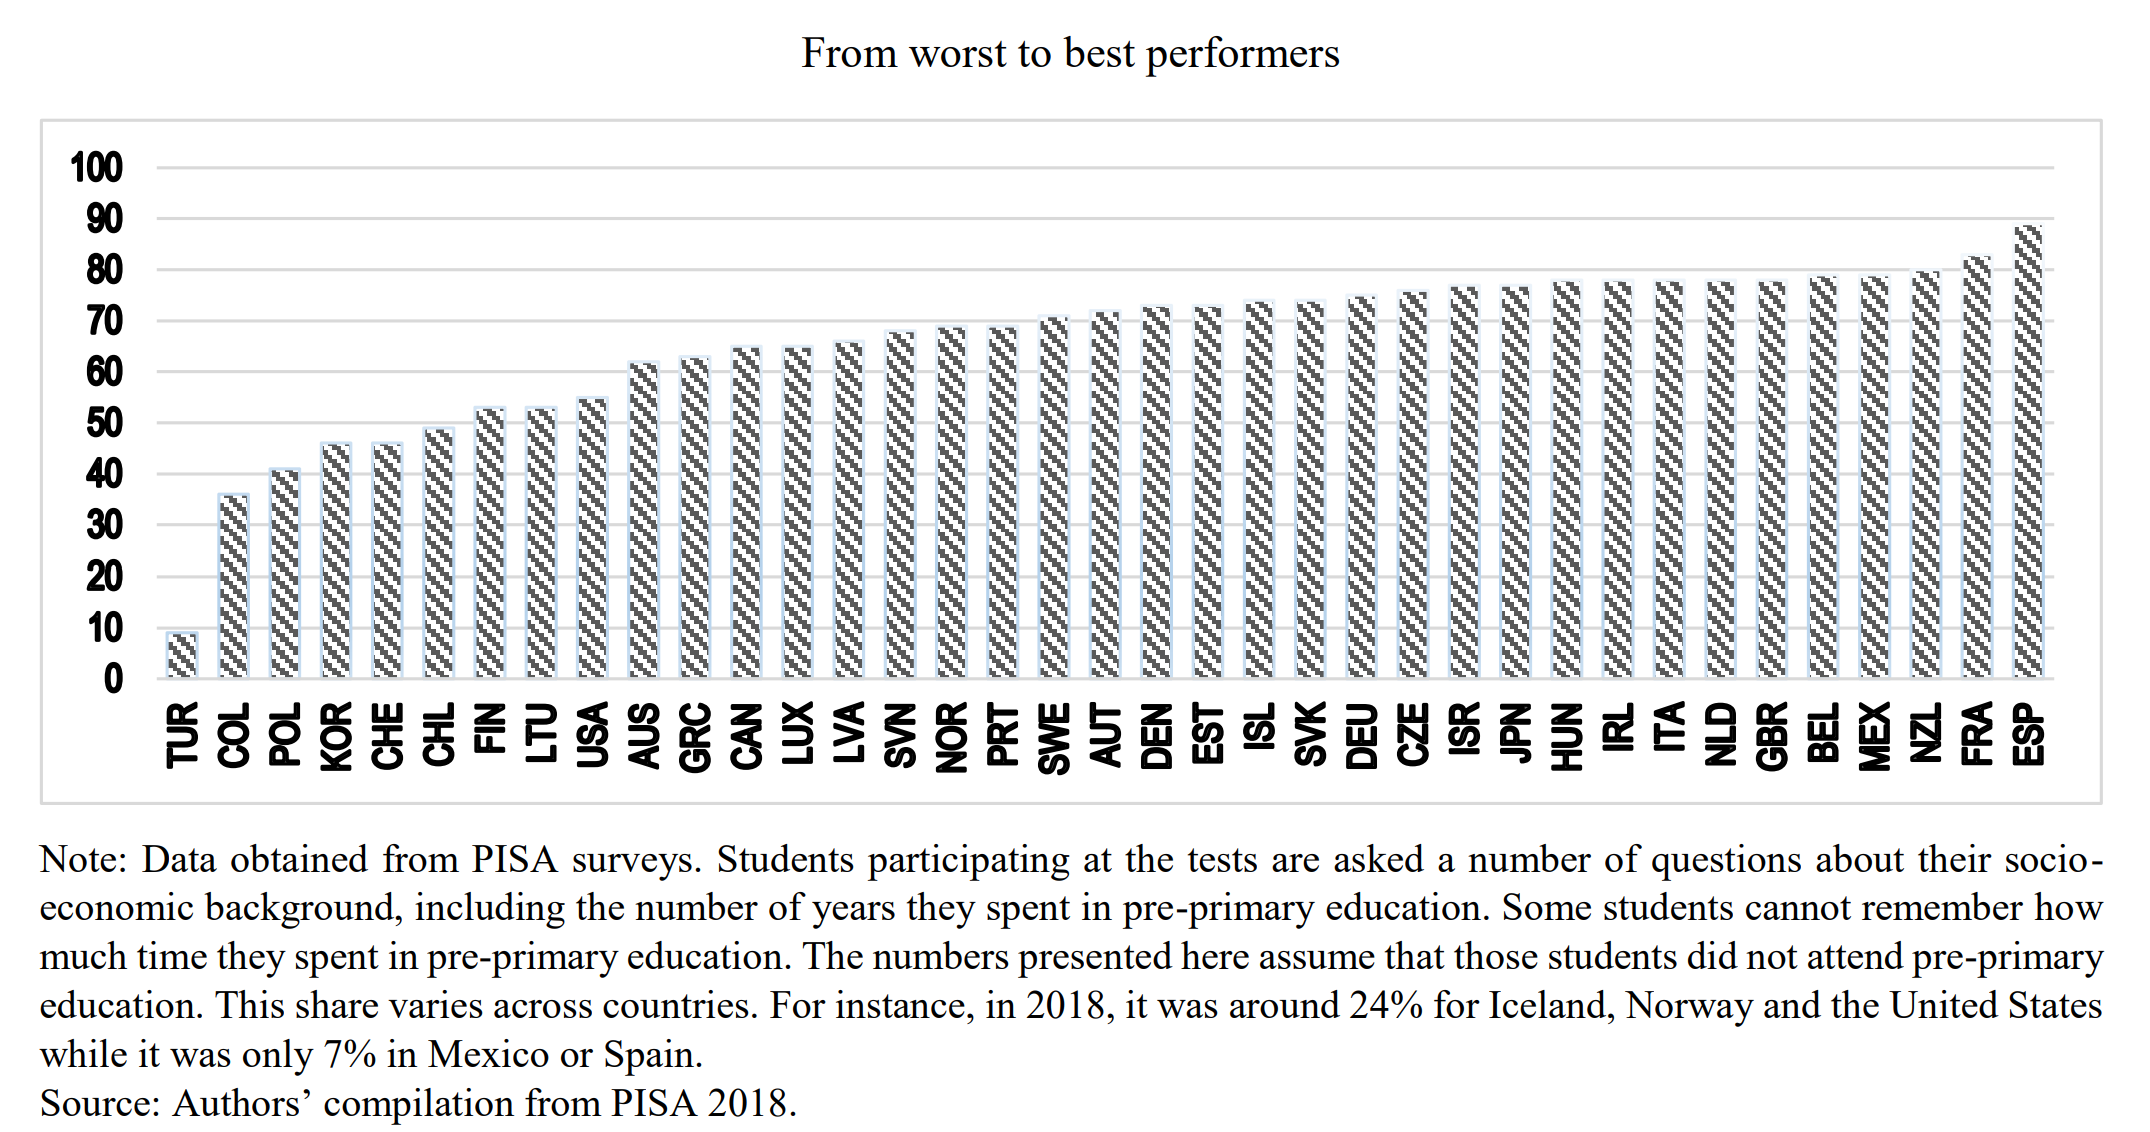
\includegraphics[width=1\linewidth]{img/growth2/egertfig7} 

}

\caption{Taken directly from Egert et al (2022) Figure 7}\label{fig:egertfig7}
\end{figure}

Egert et al.~show that improving early childhood education can have very large positive effects on future productivity. Perhaps this is not that surprising. Of course, we will have to wait a bit for these effects to kick in. After all, it will take a while for these kids to grow up and join the labor force. But good things are worth waiting for.

These effects are especially large at the bottom of the early childhood schooling distribution, where the US seems to dwell. Which of course raises the question: Why is a rich country like the US not doing more to improve early childhood intervention?

\hypertarget{technological-progress}{%
\section{Technological progress}\label{technological-progress}}

We write the production function as

\[Y_t  =  A_t F( K_t, H_tN_t)\]

where the subscript t stands for the time period and the symbols Y, A, K, H, N stand for, in order output/GDP, productivity, physical capital, human capital and labor time/ hours worked. So far, we have addressed the growth of physical and of human capital. That leaves the question:

\begin{itemize}
\tightlist
\item
  How does productivity grow?
\item
  What factors influence the growth of technology?
\item
  What factors influence technological progress?
\end{itemize}

We will use the simplest possible model to give an answer to this question.

Note that I did NOT say that I will answer this question. I said to ``provide an answer''. There are many ways to provide SOME answers.

One simple way to provide an answer is simply to assume that the new ideas that generate technological progress are created by hiring workers to create new ideas. These workers are called, surprise, surprise, scientists. We let \(S_t\) denote the number of scientists hired, then we posit that technological growth is described by

\[ \frac{A_{t+1} - A_t}{At}  =  B S_t \]

The left-hand side is the percentage growth of productivity. The right-hand side is just the resources allocated to research. This could include the number of scientists employed, perhaps weighted by their human capital, but also the labs, the buildings for the labs, the lab equipment, and supplies and energy to run the lab experiments. The relationship is very simple: The more resources allocated to science, the higher is economic growth. B is a measure of productivity in research. More precisely, as specified, this relationship is linear. A doubling of resources leads, in this specification, to a doubling of the growth rates. This is an assumption; the world does not have to look like this.

We must keep in mind that there is a feasibility or adding up constraint. There is a total number of workers in an economy. They can be either production workers or scientists/researchers who produce ideas. If we let N be the fraction of production workers and S the fraction of scientists, then we must have

\[ N + S = 1 \]

where 1 is the total number of workers. That number cannot be exceeded.

We can now take a look at technological progress in a few sectors. Perhaps the most celebrated example of technological progress is Moore's Law. Moore's law was promulgated in the early 1970s by Gordon Moore33, one of the co-founders of Intel, and meant as a forecast that the number of transistors on an integrated circuit, perhaps we can think of this as computing power, would double ever 2 years. This ``law'' stood the test of time. Over the last 40 years this relationship has held up very well. Note the scale on the vertical axis in Figure \ref{fig:growth15}. In 40 years going from 2,300 in 1971 to 2,600,000, 000. That is nothing short of spectacular.

\begin{figure}

{\centering 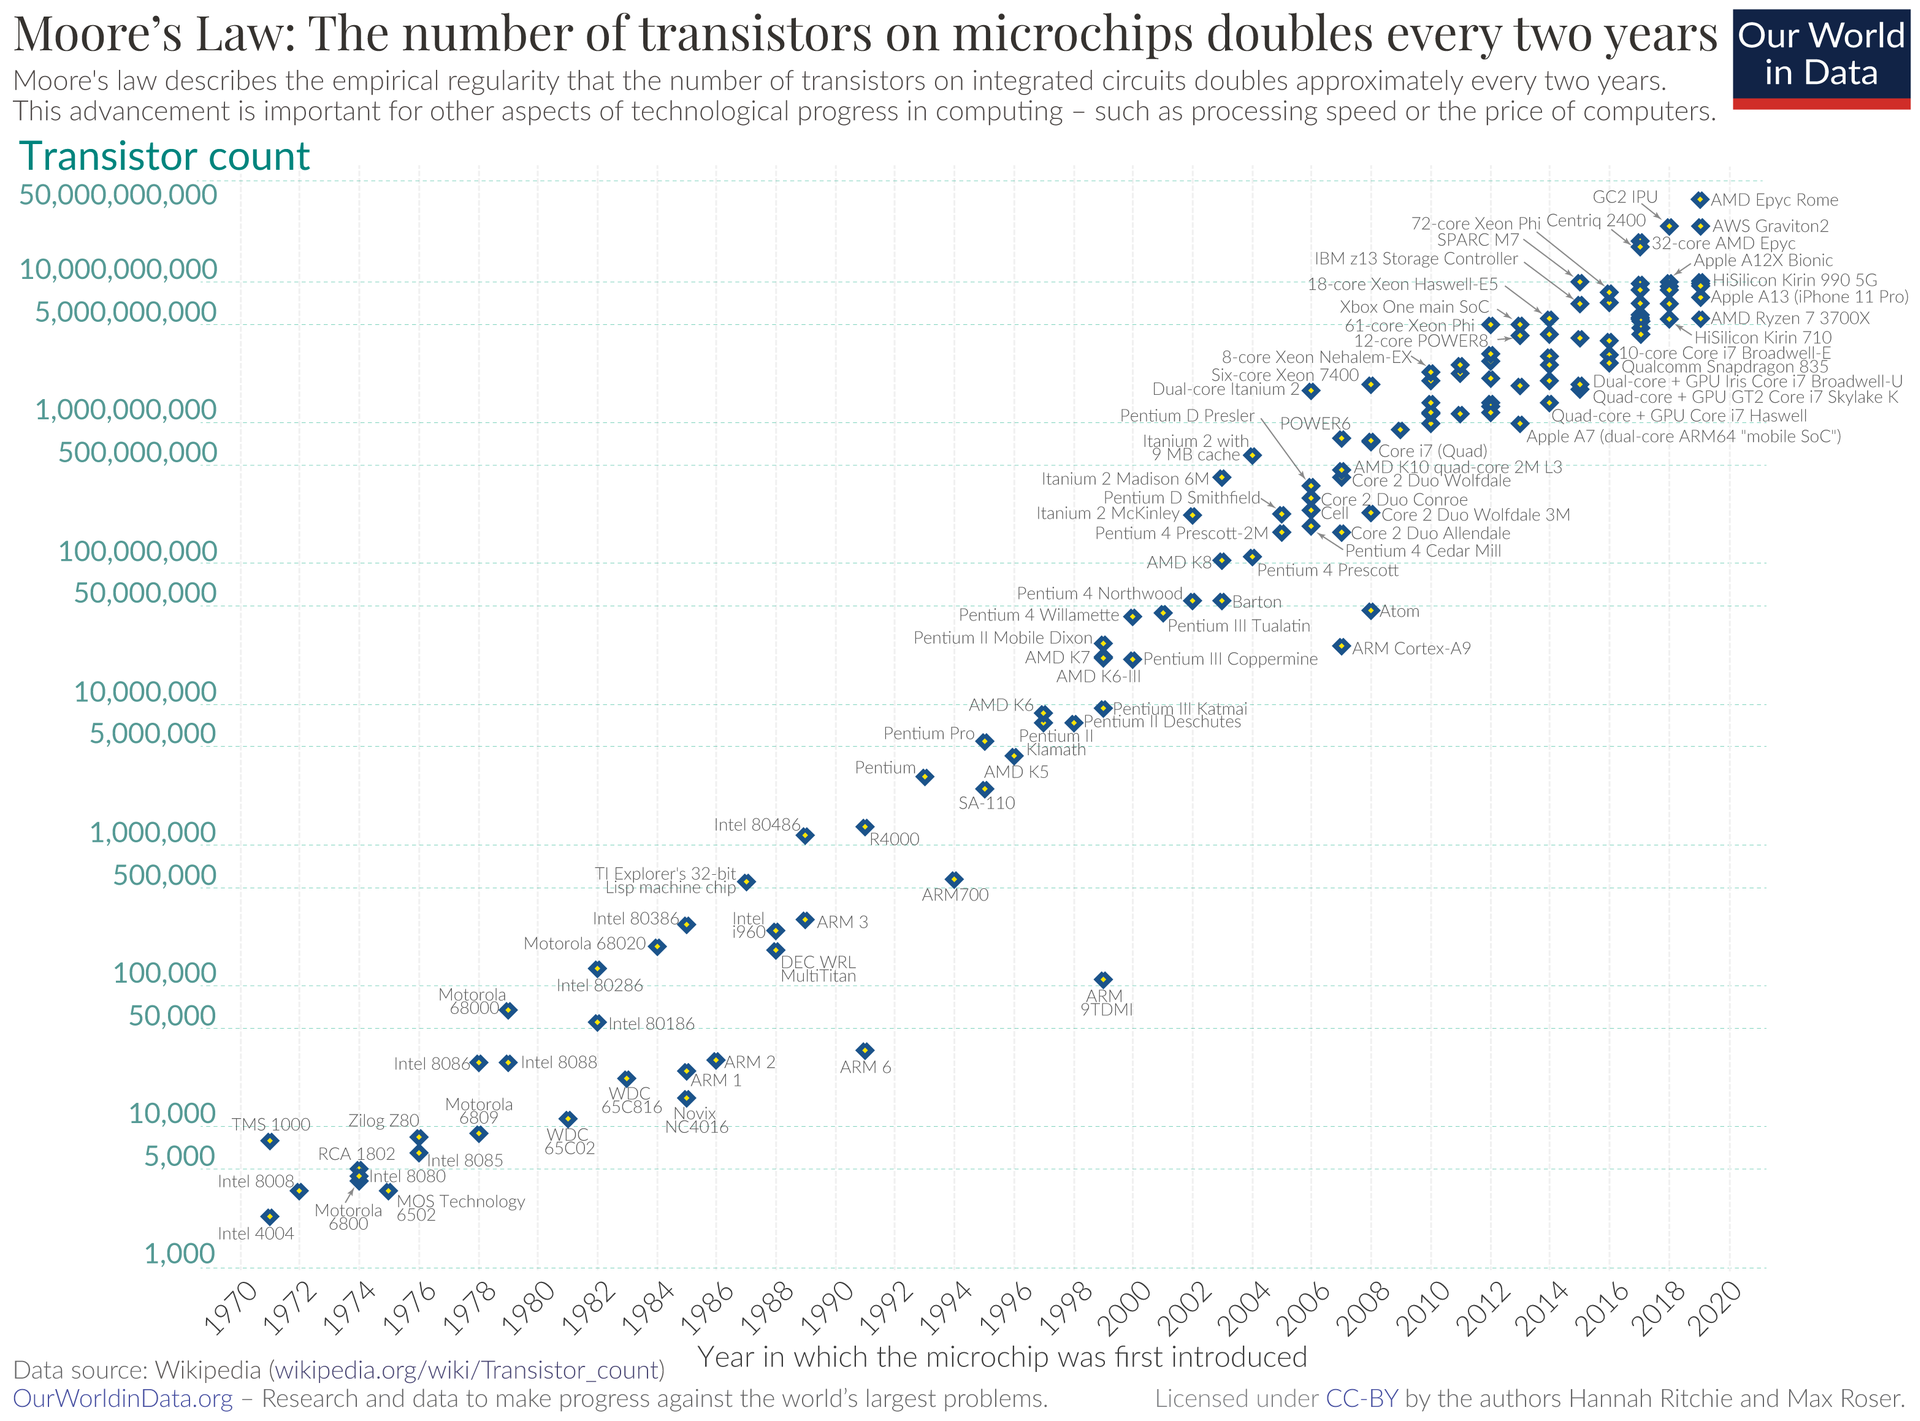
\includegraphics[width=1\linewidth]{img/growth/moore15} 

}

\caption{Moores Law}\label{fig:growth15}
\end{figure}

Considering that graph above, one could be very optimistic. There does not seem to be any break in that trend. The best fit in these data points seems to be a straight line with constant slope. Since the scale on the vertical axis is logarithmic, this looks like exponential growth at a constant rate. If there were no extra information one could become quite sanguine and expect constant exponential technological progress to continue.

Alas, there are other things to consider. What did it take to maintain the incredible growth of computing power summarized by Moore's law?

\begin{figure}

{\centering 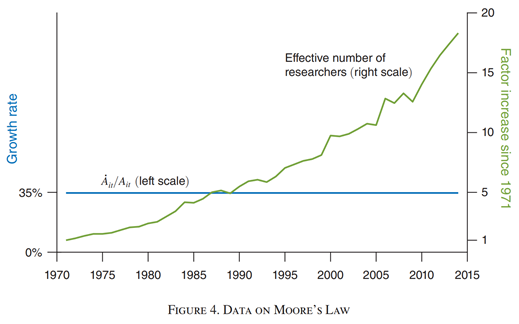
\includegraphics[width=1\linewidth]{img/growth/moore16} 

}

\caption{Moore’s law requires huge increases in the number of researchers. Source: Charles I. Jones Annu. Rev. Econ. 2022. 14:125–52.}\label{fig:growth16}
\end{figure}

Figure \ref{fig:growth16} shows that over time the number of workers/scientists required to maintain Moore's law want up by a factor of 20 over that period.

A factor of 20!

We can conclude from these two numbers that back in the 1970s, it was easier to double every two years. Now it is harder to double. It takes more resources to double.

That is diminishing returns.

There is no hint in the data, these two series in Figures \ref{fig:growth16} and \ref{fig:growth16}, that future doubling will require fewer inputs.

We picked the low hanging fruit first. Now we got to climb higher.

Figure \ref{fig:growth17} shows something similar for agriculture: Yields per acre have been growing, but at declining rates but the number of researchers has been rising tremendously. Wheat, corn, soybeans, cotton; its all the same story.

\begin{figure}

{\centering 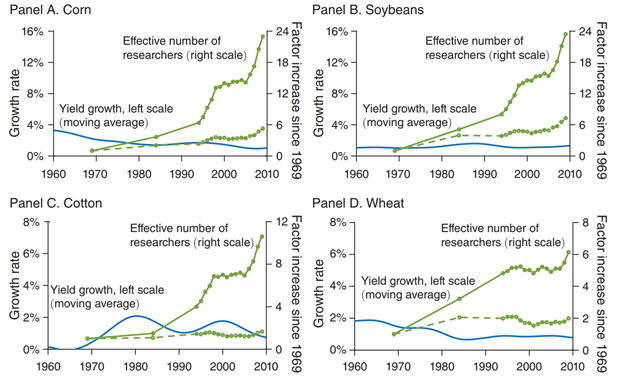
\includegraphics[width=1\linewidth]{img/growth/moore17} 

}

\caption{For agriculture it seems the same holds true. Increases in productivity come at an ever increasing resource requirement. Source: Charles I. Jones Annu. Rev. Econ. 2022. 14:125–52.}\label{fig:growth17}
\end{figure}

Low hanging fruit was picked long time ago.

Figure \ref{fig:growth18} panel b shows the same story for mortality or survival from breast cancer. Mortality rates are way down, and they are declining, albeit at declining rates. Research effort measured by scientific publications and clinical trials are way up.

\begin{figure}

{\centering 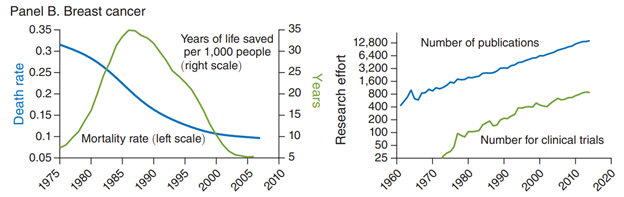
\includegraphics[width=1\linewidth]{img/growth/moore18} 

}

\caption{For health again it seems the same holds true. Increasing productivity comes at the cost of ever increasing resource requirements. Source: Charles I. Jones Annu. Rev. Econ. 2022. 14:125–52.}\label{fig:growth18}
\end{figure}

Same old song: Low hanging fruit was picked years ago.

Figure \ref{fig:growth19} shows how drastic these diminishing returns are. Peak productivity was reached around 1990 when one clinical trial was responsible for about 16 life years saved per 100,000. Now we are down to 1.

A drop from 16 to 1.

\begin{figure}

{\centering 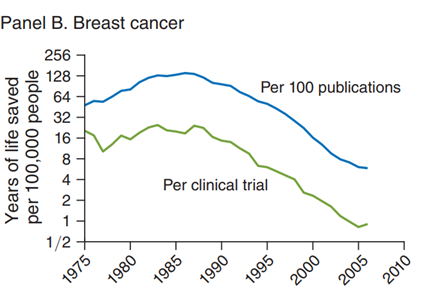
\includegraphics[width=1\linewidth]{img/growth/moore19} 

}

\caption{Diminishing returns to breast cancer after 1985. Source: Charles I. Jones Annu. Rev. Econ. 2022. 14:125–52.}\label{fig:growth19}
\end{figure}

Most low hanging fruit seems to be gone. If we want to get any fruit, we got to climb REEEEAAAAAALLLLLLY high.

Since there seem to be many industries where technological progress is only achieved with the help of ever-increasing numbers of scientists it is a fair question to ask whether this is true also in the aggregate, i.e., for the total economy.

The answer to this question is a resounding YES. Figure 1 shoes aggregate technological progress for the US economy over a 70-year period starting with the 1930s. The pattern is clear: There is no increase at all in the rate at which technology has progressed. If anything, there is a declining trend.

\begin{figure}

{\centering 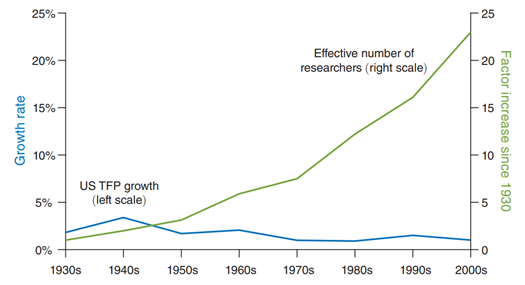
\includegraphics[width=1\linewidth]{img/growth/moore20} 

}

\caption{Constant or declining productivity growth has required ever more researchers. Source: Charles I. Jones Annu. Rev. Econ. 2022. 14:125–52.}\label{fig:growth20}
\end{figure}

Figure \ref{fig:growth20} shows that this rise in productivity (at a declining rate) has been accomplished by an increase in researchers in the order of a factor of 20! This is huge.

Just like at the level of individual industries or activities, there is no evidence that these trends will be reversed. We can, with some degree of confidence, predict that future economic growth will be lower than past economic growth.

Those politicians running for election, who promise to make the economy grow at 3 or 4 \% annually, have to work really hard to fulfill their promises since they are working against strong headwinds that are basically beyond their control.

(All the above figures are from the first paper listed below.)

The second paper below addresses the questions:

\begin{itemize}
\tightlist
\item
  What factors are contributors to the growth of real per capita GDP or output for short? And how important are they?
\item
  What factors are contributors to technological progress or the growth in productivity? And how important are they?
\end{itemize}

Given the production function specified above, we can decompose the growth in output into the following components:

\begin{enumerate}
\def\labelenumi{\arabic{enumi}.}
\tightlist
\item
  Changes in the ratio of capital to output
\item
  Changes in educational attainment/ growth in human capital
\item
  Changes in the employment to population ratio
\item
  Changes in the fraction of workers in production rather than research.
\end{enumerate}

How big is each of these factors? Jones (2021) provides the estimates. In the US starting in the 1950s, an increase in fraction of people employed is responsible for growth of 0.2\%, the increase in human capital per person is responsible for growth of 0.5\%, and technological progress contributes 1.3\% for a total of 2\% annual real per capita growth. Punchline: productivity growth or technological progress is responsible for the biggest part of growth.

What is the potential for future economic growth?

It seems difficult to imagine that educational attainment can still increase substantially. In the US, median years of schooling increased relatively rapidly until about 1980, but then the curve flattened out and that growth diminished. It is unlike that that growth will increase in the near term.

We are already hiring more and more researchers to generate more ideas with diminishing returns. Hiring more and more researchers comes at a cost of fewer workers in production with a corresponding current output decline. It seems hard to think of factors that can turn the declining research productivity around.

How about population growth? As the population grows, there are potentially more researchers as well. But population growth rates are falling worldwide?

Perhaps we can do a better job identifying and fostering future Einsteins and Curies? According to some estimates only 12\% of inventors are women, while roughly half of the population is women. Policies that increase that number might increase growth by 0.3\%.

\url{https://web.stanford.edu/~chadj/dignity.pdf}

\url{https://web.stanford.edu/~chadj/annualreview.pdf}

\hypertarget{nails}{%
\section{Nails}\label{nails}}

Sometimes we see something very extra ordinary in something totally ordinary. But I think that is true in life in general. Sometimes we see it. Sometimes we don't.

Nails are very ordinary. Our lives are made much better by nails. All of our kitchen cabinets, let alone our houses, are all held together by nails.

So, what is so remarkable about nails?

It is the prices!

Sichel (2022) has pit together a long data series on nail prices. See Figure \ref{fig:sichelfig2} below.

\begin{figure}

{\centering 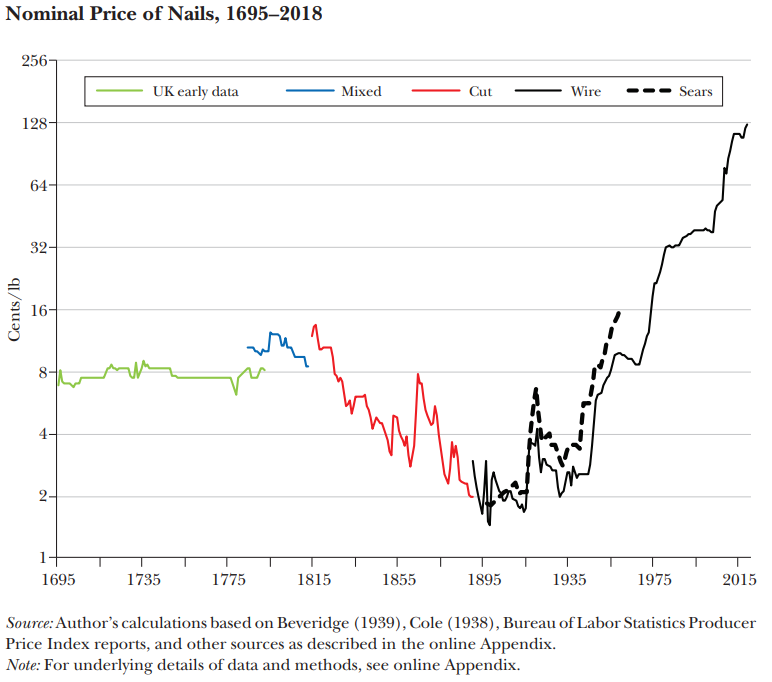
\includegraphics[width=1\linewidth]{img/growth2/sichelfig2} 

}

\caption{Taken directly from The Price of Nails Since 1695: A Window into Economic Change by Daniel Sichel (Journal of Economic Perspectives 2022), Figure 2 }\label{fig:sichelfig2}
\end{figure}

But you will say: what is unusual about this? The price is kind a constant, then drops then rises. We all know that prices always fluctuate.

But let us not been that dismissive that quickly. The prices in that figure are nominal prices. We should probably correct for inflation and for changes in nail quality. Nail quality would be something like ``holding power''.

If we do this, we get a series of nail prices as in Figure \ref{fig:sichelfig4}.

\begin{figure}

{\centering 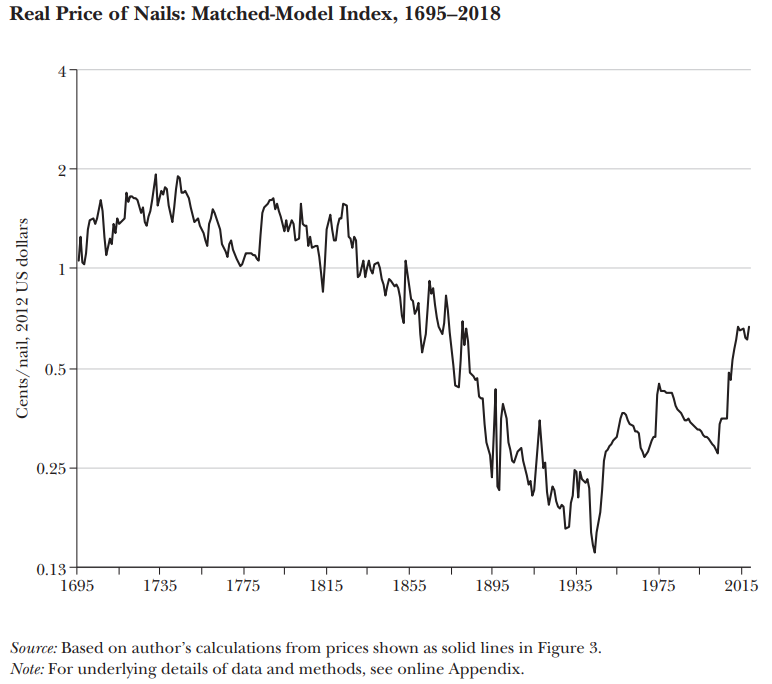
\includegraphics[width=1\linewidth]{img/growth2/sichelfig4} 

}

\caption{Taken directly from The Price of Nails Since 1695: A Window into Economic Change by Daniel Sichel (Journal of Economic Perspectives 2022), Figure 4 }\label{fig:sichelfig4}
\end{figure}

The drop in prices between 1695 and 1935 is spectacular: The price has dropped from almost 2 cents a nail to about 0.15 cents a nail. That is drop by a factor of 10!

Why would the price drop so much?

There typical reasons are:

\begin{itemize}
\tightlist
\item
  The availability and prices of inputs in the production of nails.
\item
  The quality of such inputs.
\item
  Total factor productivity.
\end{itemize}

So, what is the lions' share of the reasons for this large drop in the price of nails? It is total factor productivity. That factor is so large that it totally overwhelms the other factors. The periods where total factor productivity really had its biggest kick are the periods where rapid technological change happened such as the switch from steam to electricity.

\hypertarget{light}{%
\section{Light}\label{light}}

\url{https://www.nber.org/system/files/chapters/c6064/c6064.pdf}

What a miracle. You wake up in the morning in January and you flip a switch, and voila, you can see, dimly because you are not quite awake, but you can see; you can see because there is light.

It has not always been like that. Our early ancestors struggled mightily to get some light by making a fire so they could see.

Over thousands of years things have changed and improved. We went from collecting firewood and rubbing stones together to flipping a switch.

These technological advances involved changes from the open fires to lamps, to candles, to gas and petroleum, to electric lighting, and from carbon to tungsten filaments.

These historical developments are listed in Table \ref{fig:nordhaustab1p3} below

\begin{figure}

{\centering 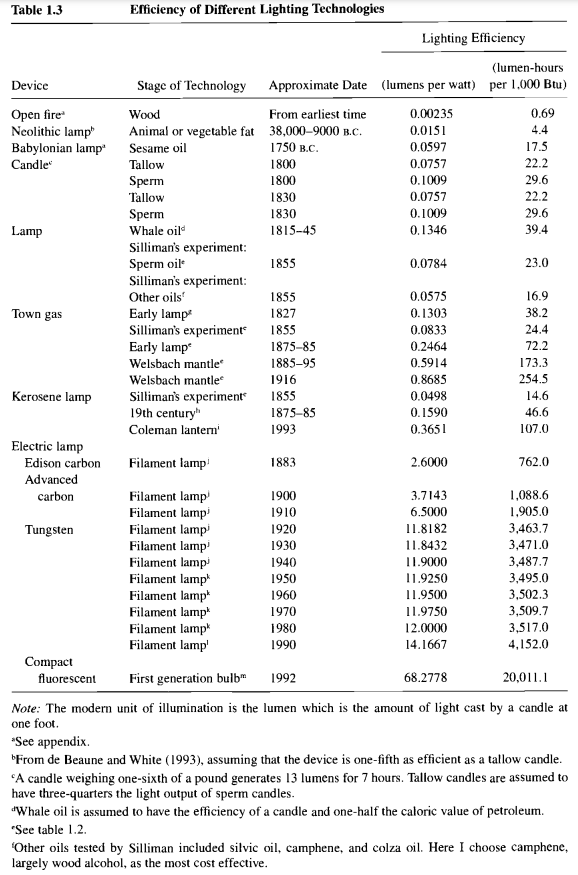
\includegraphics[width=1\linewidth]{img/growth2/nordhaustab1p3} 

}

\caption{Taken directly from Do Real-Output and Real-Wage Measures Capture Reality? The History of Lighting Suggests Not by William D. Nordhaus (NBER 1996), Table 1.3}\label{fig:nordhaustab1p3}
\end{figure}

Before we follow the historical development of these technological improvements, we need to fix few terms.

\begin{itemize}
\tightlist
\item
  Light is radiation that stimulates the retina.
\item
  Light flux or flow is the rate of emission from a source.
\item
  The unit of light flux is a lumen.
\item
  The unit of illuminance, the amount of light per unit area, is the lux.
\end{itemize}

All of this is physics so far. We need to get to the economics\ldots{}

We are interested in the price of a lumen hour. The price is an imperfect measure.

There are many factors which influence the price. There are input prices that can increase or decrease over time. There is technological change. Getting the price changes right is crucial. The price of light of course depends on the price of inputs. Between 1883 and 1983, the price of gas and kerosene rose by a factor of 10 and the price of electricity fell by a factor of 3!

Adjusting for quality is another major issue. Just imagine sitting by the light of two candles in the UK in the 1700s and doing your algebra homework. Or imagine your parents paying a slew of medical bills over an open fire pit.

If you do all these things carefully, you can constrict price of light data for the last 200 years. This is exactly what Nordhaus did in 1996. His results are in Figure \ref{fig:nordhausfig1p3} below.

\begin{figure}

{\centering 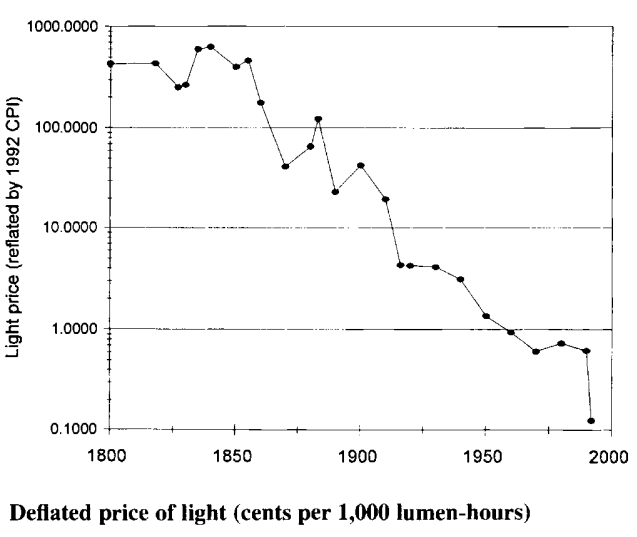
\includegraphics[width=1\linewidth]{img/growth2/nordhausfig1p3} 

}

\caption{Taken directly from Do Real-Output and Real-Wage Measures Capture Reality? The History of Lighting Suggests Not by William D. Nordhaus (NBER 1996), Figure 1.3}\label{fig:nordhausfig1p3}
\end{figure}

That is an impressive drop. From almost 1000 to about 0.1.

Three cheers for technological progress!

\hypertarget{additive-growth}{%
\section{Additive Growth}\label{additive-growth}}

So far the basic underlying assumption in everything we have done is that

\begin{center}
growth is exponential.

\end{center}

A recent paper by Philippon (2022) casts grave doubt on this assumption. We briefly lay out his main arguments here.

Imagine that technological progress is the main driver of economic growth. We can and we have modelled technological progress as

\begin{equation}
\frac{A_{t+1}}{A_t}=A_t(1+g)
\label{eq:techmult}
\end{equation}

Here, of course, \(A_t\) is the level of technology and \(g\) is a positive number. This equation just says that the growth rate of technology takes the current level of technology and multiplies it by some number. This is all well and good and it sounds very reasonable. And a bunch of economic research going back all the way to Solow (1956) has made and used this assumption.

But:

It would just have been as reasonable to assume and write

\begin{equation}
\frac{A_{t+1}}{A_t}=A_t + b
\label{eq:techadd}
\end{equation}

Equation \eqref{eq:techmult} is multiplicative; Equation \eqref{eq:techadd} is addititve.

There is no ``a priori'' (you may want to look this up) reason to believe that one of those two equations is a better assumption for research on economic growth than the other.

So how do we distinguish one model, one assumption, one theory from another?

We use data. At least we try to use data.

This is the approach social scientists take in many areas of live: using data to distinguish theories.

Here is another example:

Suicides by incidence in the US is very high.

Theory 1: It is a mental health problem.

Theory 2: It is a gun availability problem.

Question: What is the best data you can use to distinguish between these two theories?

Back to growth.

How does Philippon (2022) use data to distinguish Equations \eqref{eq:techmult} and \eqref{eq:techadd}?

First, he takes data on total factor productivity (TFP) the \(\{A_t\}\) series in the models for the US from 1947 to 2019. He hires two statisticians, George (for geometric growth), and Daniela (for addititive growth). He gives them the sample from 1947 to 1983 and asks them to forecast the data up until 2019.

Their answers are below in Figure \ref{fig:philipponfig1}

\begin{figure}

{\centering 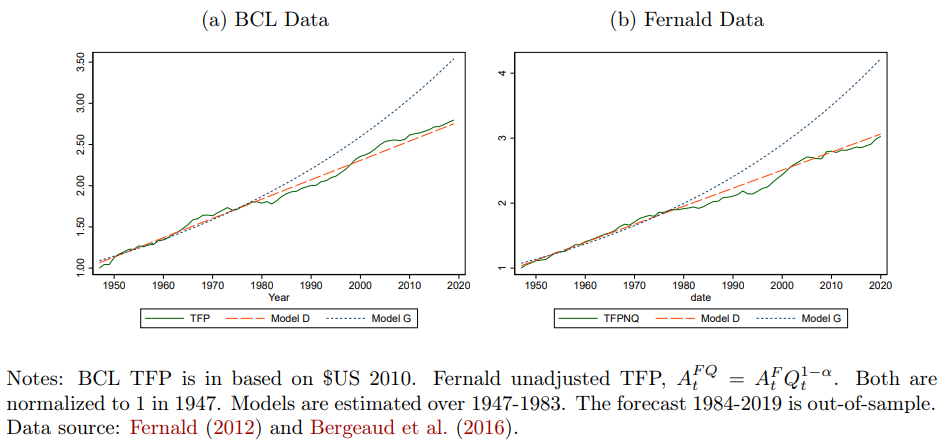
\includegraphics[width=1\linewidth]{img/growth2/philipponfig1} 

}

\caption{Taken directly from Additive Growth by Thomas Philippon (NBER 2022), Figure 1}\label{fig:philipponfig1}
\end{figure}

The data (reality) is the solid line. George's forecast is exponential (Equation \eqref{eq:techmult}) and is way off.

It appears that Daniela's forecast, using Equation \eqref{eq:techadd} is much better.

But growth here in it's additive form is not constant over very long horizons. Consider Figure \ref{fig:philipponfig4} below

\begin{figure}

{\centering 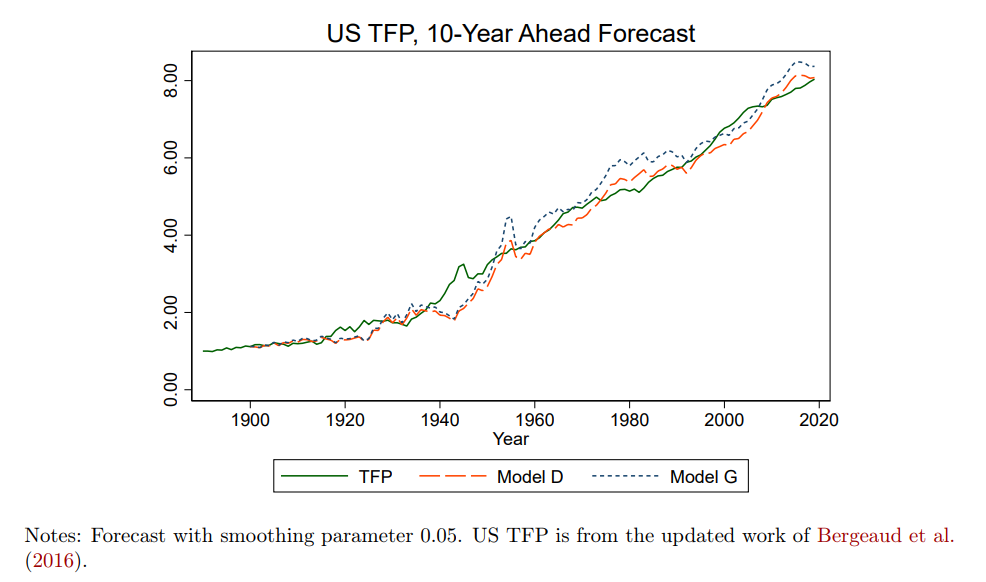
\includegraphics[width=1\linewidth]{img/growth2/philipponfig4} 

}

\caption{Taken directly from Additive Growth by Thomas Philippon (NBER 2022), Figure 4}\label{fig:philipponfig4}
\end{figure}

There is a definite break in the data in the 1930s. Field (2003) argues that

\begin{quote}
``the years 1929-1941 were, in the aggregate, the most technologically progressive of any comparative period in US economic history.''
\end{quote}

Perhaps this timing is a bit of a puzzle since what we consider to be many of the great drivers of technological progress, electric light, electric power, and the internal combustion engine were all discovered much, much earlier.

But the 1930s were a period of great ``follow-on inventions, such as the perfection of the piston power-powered aircraft and television, and the increasing quality of machinery made possible by the large increases in available horsepowers and kilowatt-hours of electricity.'' (Philippon 2022, p26) These follow-on inventions powered technological progress since.

The punchline: The constant average additive growth after the 1930s is over three times as high as before that period.

All the way to the year 2020.

Why does any of this matter?

There has been much talk, discussion, punditing, and even economic research on

\begin{center}
the productivity slowdown.

\end{center}

And along with this discussion of the productivity slowdown, come all kinds of well and ill informed policy proposals:

\begin{center}
Change education

Lower Taxes

Ease the Regulatory Burden

Etc.

Etc.

Etc.

\end{center}

IF growth is not exponential, IF growth is indeed linear, then Phillipon says

\begin{center}
\textbf{There is no productivity slowdown}

\end{center}

and all the above policy discussions are moot.

\hypertarget{glossary-of-terms-2}{%
\section{Glossary of Terms}\label{glossary-of-terms-2}}

\textbf{Human Capital:} the stock of marketable skills of the labor force in a country.

\textbf{Technological Progress:} increase in total factor productivity.

\hypertarget{practice-questions-2}{%
\section{Practice Questions}\label{practice-questions-2}}

\hypertarget{discussion-2}{%
\subsection{Discussion}\label{discussion-2}}

\hypertarget{multiple-choice-2}{%
\subsection{Multiple Choice}\label{multiple-choice-2}}

\begin{enumerate}
\def\labelenumi{\arabic{enumi}.}
\item
  The best measure of human capital in an economy is

  A. The fraction of workers with a college degree\\
  B. The fraction of workers with a high school degree\\
  C. Test scores of students in math and science\\
  D. The high school drop out rate
\item
  The best measure of human capital in the labor force in United States in the year 2015 is

  A. Test scores in math and science of workers who entered the labor force in 2010\\
  B. Test scores in math and science of workers who entered the labor force in 1970\\
  C. Test scores in math and science of workers who entered the labor force in 1950\\
  D. Test scores in math and science of workers who entered the labor force between 1970 and 2010
\item
  In the data set used by Hanushek and Kimko (2000) which pairs of data across countries are correlated

  A. Education expenditure per student and test scores\\
  B. Education expenditure per student and growth rates of GDP\\
  C. Growth rates of GDP and test scores\\
  D. Growth rates of GDP and median years of schooling, after correcting for the math and science scores
\item
  If the process of economic growth is linear as claimed by Philippon, then the percentage growth rates over time will be

  A. Increasing\\
  B. Decreasing\\
  C. Constant\\
  D. Oscillating
\item
  Imagine that in the years 1980, 1990, 2000, 2010 and 2020 the 5 year mortality rates from colon cancer are 45\%, 40\%, 35\%, 30\% and 25\%, respectively. The number of researchers employed in these years is 100, 110, 121, 133, 147. If we consider the percentage reductions in mortality rate the research output, then this example displays

  A. Constant returns to research\\
  B. Decreasing returns to research\\
  C. Increasing returns to research\\
  D. Initially increasing and then decreasing returns to research
\item
  Imagine that human capital and physical capital are equally important in the production of output. The growth rate of human capital is 4\% per year and the growth rate of physical capital is 2\% per year. Then the annual growth rate of output will be in percent

  A. 2\\
  B. 3\\
  C. 4\\
  D. 5
\item
  Imagine that physical and human capital are constant over time and that there are diminishing returns to research. Then we should expect

  A. GDP growth rates to decrease over time\\
  B. GDP growth rates to stay constant over time\\
  C. GDP growth rates to increase over time\\
  D. GDP growth rats to fluctuate over time
\item
  Imagine that the stock of physical capital grows at 2\% annually, that the stock of human capital is constant. If there are diminishing returns to research, then we would expect that

  A. The growth rate of GDP converges to 2\% over time\\
  B. The growth rate of GDP is constant at 2\%\\
  C. The growth rate of GDP converges to 0\% over time\\
  D. The growth rate of GDP converges to 3\% over time
\item
  Which one does not belong

  A. A new and improved surgical instrument\\
  B. A more fuel efficient car\\
  C. Better graphics for video games\\
  D. More varieties of soft drinks
\item
  Which one does not belong

  A. Electricity\\
  B. A fork lift\\
  C. A warehouse\\
  D. An algorithm
\end{enumerate}

\hypertarget{decisions-rational-or-irrational}{%
\chapter{Decisions: Rational or Irrational?}\label{decisions-rational-or-irrational}}

In this chapter you will learn:

\begin{itemize}
\tightlist
\item
  The basics of a simple model of rational choice
\item
  The concepts of marginal costs and marginal benefits
\item
  The concept and applications of opportunity cost
\item
  The concept of diminishing returns
\item
  The concept of increasing returns.
\end{itemize}

\hypertarget{goals-and-constraints}{%
\section{Goals and Constraints}\label{goals-and-constraints}}

In this section we will construct our workhorse model/theory that we will use in the rest of the term. We will learn about the notion of rationality that is commonly used in economics. We will learn what rationality means and we will learn what choices are like if they are governed by rationality.

Rationality always begins with the assumption of a goal or of an objective. We assume that all of our behavior is guided by goal, that all of our behavior is purposeful or goal oriented. Our goals will vary from person to person. There is no reason to believe that your goals should be the same as my goals. We simply accept whatever goals individuals might have. And we do not judge them. We recognize that our individual goals may vary from time to time.

Leslie's goal is to get elected to Congress. Jack's goal is to graduate from IU with at least a 3.7 grade point average with a major in economics and a minor in computer science. George's goal is to slay the dragon. Georgina's goal is to be able to retire at age 49 with a retirement portfolio valued at least at 4 million dollars.

Our goals can change overtime. As Georgina realizes at age 40 that she is far away from her goal she might adjust her goal of retiring to age 55. Sometimes we set aside some goals completely and work on other goals almost exclusively.

Joanne wants to be valedictorian in her high school. She is a varsity soccer player. During the soccer match on Saturday afternoon, she does not even think about her English project or her chemistry lab; she only thinks about the soccer match. During those 90 minutes her goal of being valedictorian does not enter her mind at all; the only thing that matters to her in those 90 minutes is winning the game.

In pursuit of our goals, we are typically limited by a variety of constraints:

\begin{itemize}
\item
  First: There is a budget or financial constraint. That 10 million dollar mansion in Malibu overlooking the Pacific is not in my budget. Nor is the luxurious trip around the world in 180 days. Most of us are facing this type of budget constraint. Perhaps if you are Elon Musk you don't feel it as much as the average IU student.
\item
  Second: Most of us face time constraints. There are only 24 hours in a day. Sometimes these time constraints are more binding, or at least they feel more binding than at other times. If we go on a nice vacation with our family, hanging out at the beach, watching the waves gently lap on the sandy beach, time seems to stand still, there is no rush and we might well ask: A time constraint? What is that? But our life is not like that all of the time. Just think of the parents who are rushing to fill out their tax forms late on April 14th. That is crunch time. Or think of your own situation as you are preparing for four difficult final exams while two projects are due and while the university is asking you to move out of your dorm room within 36 hours of your last exam. That is also crunch time. Then the time constraint bites, it really bites.
\item
  Third: Most of us are facing constraints that have to do with our intellectual bandwidth. How much can we compute or calculate? How many hundreds of pages can we read over the weekend for a project in our history class and fully comprehend what we read? Evidently, in chess one secret to success is to be able to figure 8, 10, 12, or 15 moves ahead including how the adversary will respond to each one of our moves. Some of us have that gift, that large bandwidth. I certainly don't.
\item
  Fourth: Many of us in some points in our lives will face emotional constraints. People experiencing poverty often live in the tyranny of the moment, going from one crisis to another. The mom with two young children who has struggled all her life to make ends meet and who just found out that her husband has abandoned her might well be at the end of her rope and ask: how much more can I take? She is facing severe emotional constraints.
\end{itemize}

Some constraints are technological. They just say that certain things are physically impossible. One of my dreams has been to climb Kilimanjaro, but I think I have to face the fact that at my age and in my physical condition that is impossible. There are many such a technological constraint.

A nice example of such a technological constraint is illustrated in Figure 1 below. It is recognized that between 1960 and 2010 computing power has doubled every two years. That sounds like a fantastic achievement. That is just Moore's Law.

\begin{figure}

{\centering 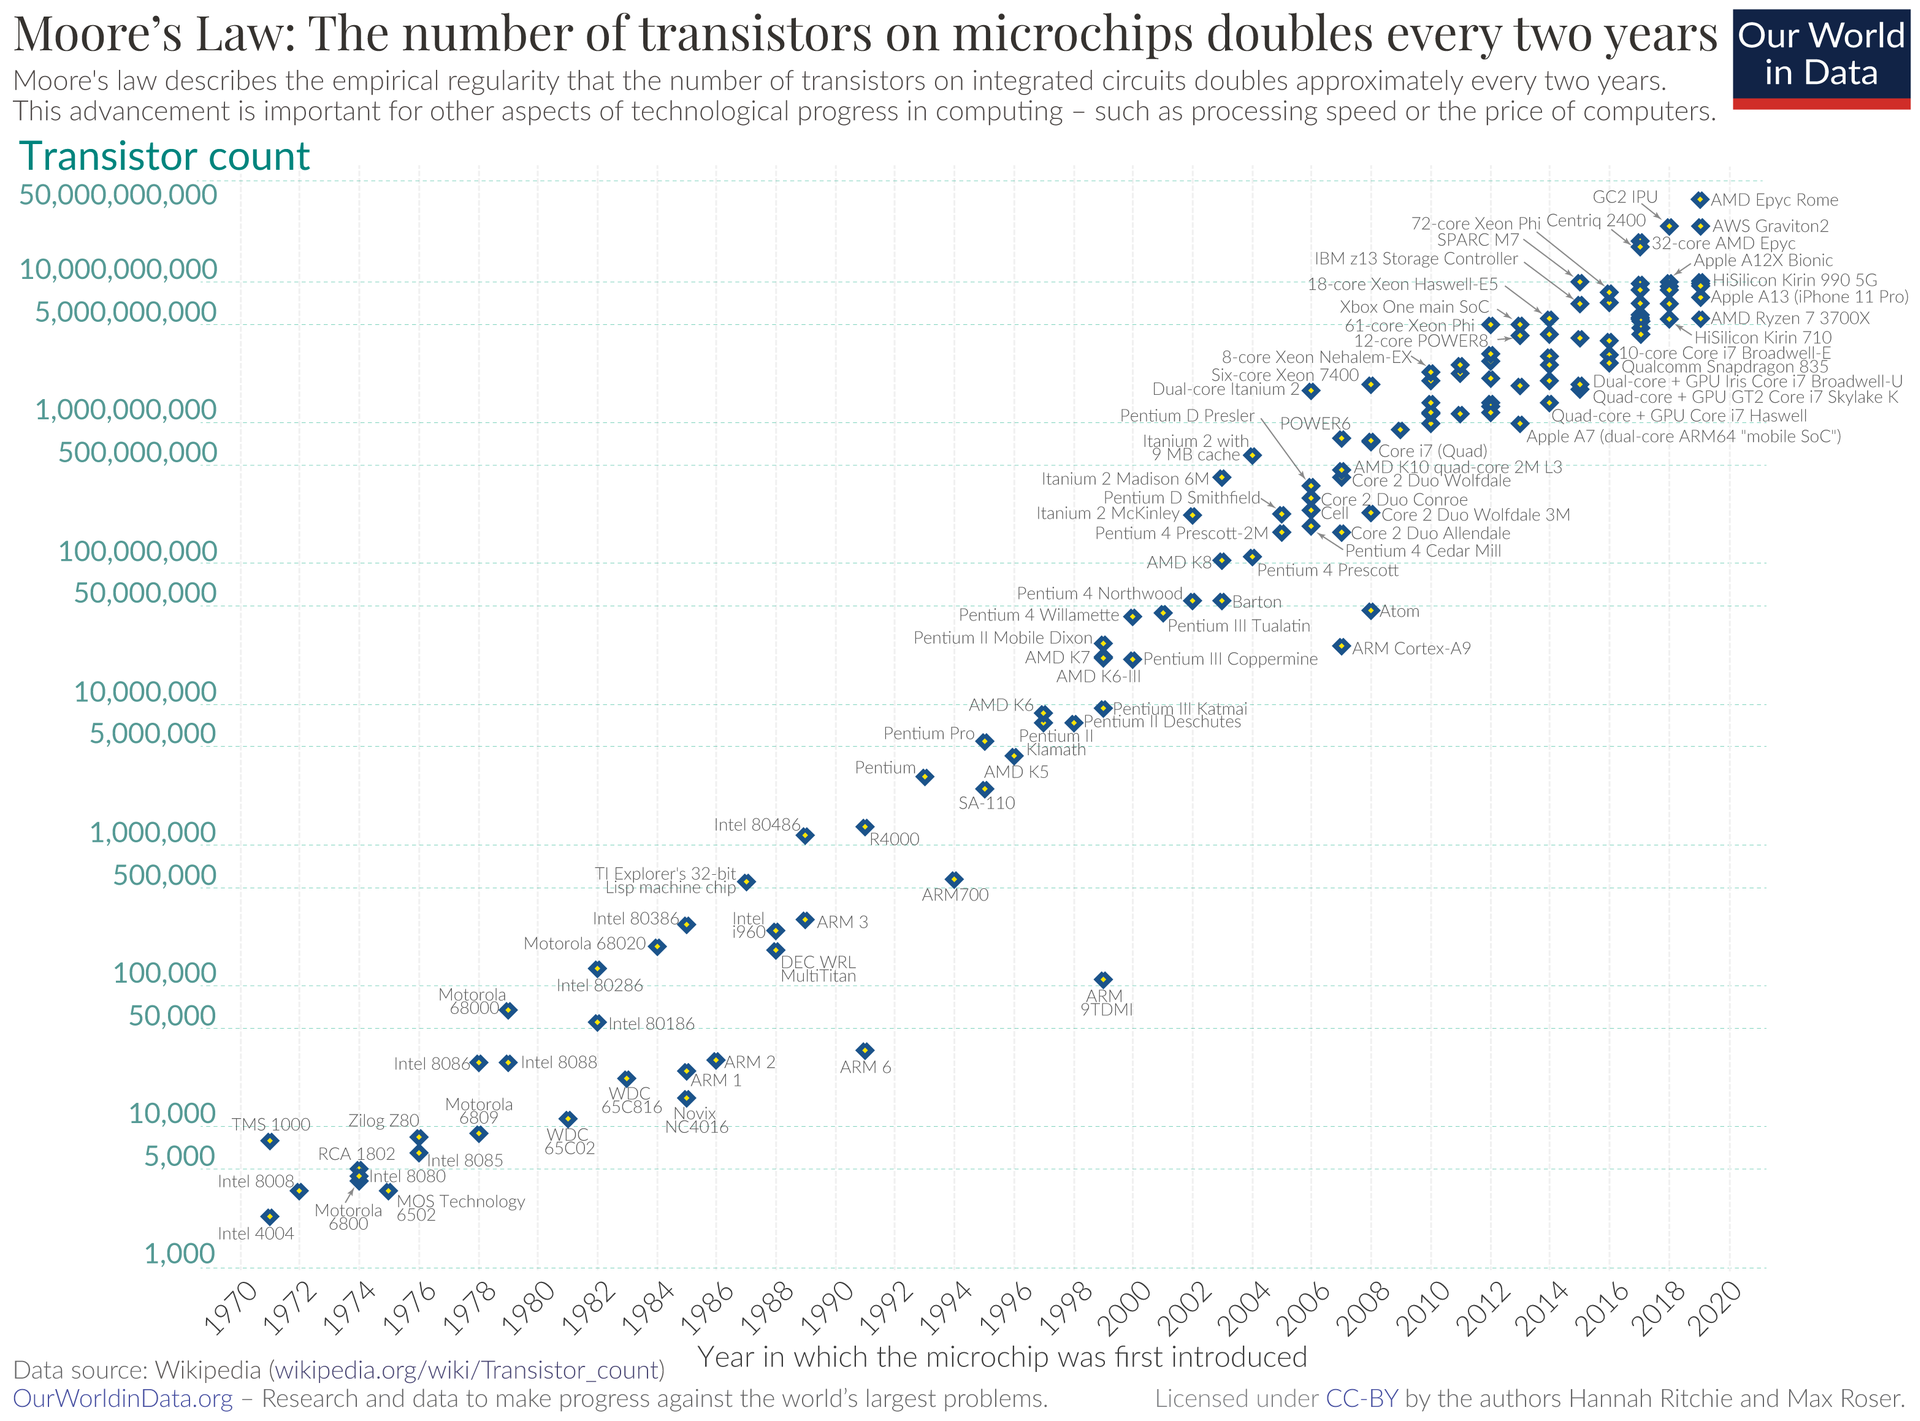
\includegraphics[width=1\linewidth]{img/rationalchoice/moore} 

}

\caption{Moores Law}\label{fig:rationalchoice1}
\end{figure}

It turns out that for some purposes the doubling of computing power every two years is not enough. In order to train systems of artificial intelligence, AI, well, a doubling of computing power every 3 to 4 months seems to be required. Good luck with speeding up the growth of computing power by a factor of 6!

\begin{figure}

{\centering 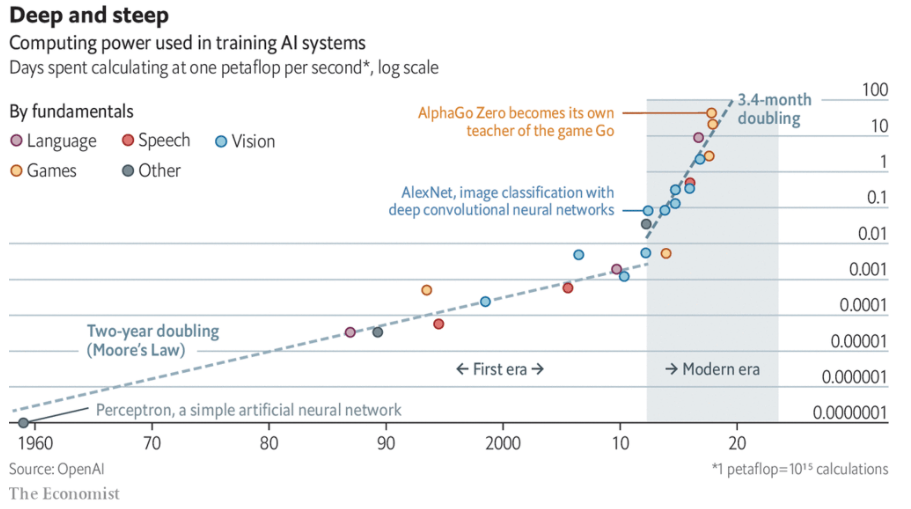
\includegraphics[width=1\linewidth]{img/rationalchoice/mooredeepandsteep} 

}

\caption{Source: The Economist, "The cost of training machines is becoming a problem" July 13, 2020.}\label{fig:rationalchoicemooredeep}
\end{figure}

\hypertarget{marginal-costs-and-benefits}{%
\section{Marginal Costs and Benefits}\label{marginal-costs-and-benefits}}

We will now illustrate the foundations for a model of rational choice. Whenever we make a choice we weigh, if we are rational, the costs of the action and the benefits of the action. We will start with an action that can be chosen in small increments.

Examples of such actions are:

\begin{itemize}
\tightlist
\item
  How many miles do I want to hike this coming weekend?
\item
  How much money do I want to contribute to a charity?
\item
  How much time do I want to spend texting my parents while I'm getting ready for my exam in college?
\item
  How much time do I want to study for the final in my introductory economics course?
\item
  How much chocolate do I want to eat this week?
\end{itemize}

In all of these cases, the choice is a continuous variable, the choice is not a discrete, all or nothing kind of choice.

Of course, there are many choices that are of the all-or-nothing variety:

\begin{itemize}
\tightlist
\item
  Getting on an airplane to fly to San Diego during Covid-19: yes or no?
\item
  Attending IU: yes or no?
\item
  Marrying my high-school sweetheart: yes or no?
\end{itemize}

In a sense, the all or nothing choices are relatively easy to model and understand. If you think you are better off marrying your high school sweetheart than not, then, by all means, marry your high school sweetheart. In econ speak: if the benefit of marrying your highschool sweetheart exceeds the cost, then go ahead and marry your high school sweetheart. (Of course, it takes two to tango!)

The decisions where continuous choices are involved might be somewhat harder to model. This is what we are embarking on now. We need some terminology.

The marginal benefit of an action, MB, is the extra benefit obtained by carrying out the action one more unit.

The marginal benefit of hiking one extra mile is the enjoyment I get out of being in nature for another 20 to 30 minutes or so. And, of course, it is the extra calories I burn by hiking one extra mile so I can eat more cookies when I get home.

The marginal benefit of studying for the exam in my economics class is the extra understanding of the material I gain, and it includes the increased probability that I ace the exam.

The marginal benefit of talking to my mom on the phone for an extra half-hour is simply the enjoyment of communicating with my mom and it could include some extra probability of getting my allowance increased.

The marginal cost of an action, MC, is the extra cost incurred by carrying out the action one more unit.

The marginal cost of hiking one extra mile includes a bunch of things. In that extra time, 20 or 30 minutes, I could be doing all kinds of other things, like sitting on my back porch and eating cookies. If I hiked an extra mile, I might get so tired that I lose concentration, stumble over a rock or a root, fall and break an ankle. If I hiked an extra mile, I run an extra risk of getting lost and I might not be able to get back home on time for an important appointment.

The marginal cost of studying an extra hour for the exam in my economics class includes not studying for the exam in my chemistry class and it includes things like watching TV or hanging out with my friends.

The marginal cost of communicating with my mom on the phone includes not studying for my economics exam.

You get the idea. If I commit sometime to one particular action, there are a whole bunch of other things I cannot do at the same time. If I donate \$100 to one charity, I cannot donate it to another charity. If Jose works in industry 1, he cannot work in industry 2.

This brings us to the notion of opportunity cost.

Opportunity cost is one of the most important concepts in economics, if not the single most important one, and it is crucial that we have a firm grasp off this concept.

The definition of opportunity cost is simply: the value of the next best alternative forgone by making a particular choice.

Let's consider the following possibilities ranked in order pleasure or utility I derive from them:

\begin{enumerate}
\def\labelenumi{\arabic{enumi}.}
\tightlist
\item
  reading a good book
\item
  reading the New York Times
\item
  reading a letter from my son
\item
  going for a walk
\item
  talking to my brother on the phone
\item
  cleaning the gutters on my roof
\end{enumerate}

And there are many others. If these are really listed in order of priority and importance for me, I will choose reading a good book.

What is the opportunity cost of reading a good book? It is not the pleasure I get out of talking to my brother on the phone. That is the fifth best thing I could be doing at that moment. The opportunity cost of reading a good book is reading the New York Times. Reading the New York Times is my next best alternative after reading a good book. So, the opportunity cost of reading a book is the value I would have derived from reading the New York Times, my second-best alternative forgone.

\hypertarget{choice}{%
\section{Choice}\label{choice}}

We will now present our basic and simple model/theory of rational choice. We make two assumptions.

\begin{center}
\textbf{Assumption 1: The marginal benefit of an action, MB, is declining as the action is increased.}

\end{center}

When we graph the marginal benefit of an action it will be downward sloping. In Economics this assumption is known as

\begin{center}
Diminishing returns
or
Diminishing utility

\end{center}

This is an assumption, not a universal law, that makes sense in many situations, but not in all. We will address some exceptions later on. But in many situations, this makes sense.

After cutting grass in my backyard on hot Saturday in July, the first sip or glass of sweetened iced tea just tastes great and quenches my thirst. The second glass a little bit less, the fourth glass not so much.

That first hour of a hike on a mild fall day feels wonderful. By the third hour I feel tired and my back hurts from carrying a backpack.

Seeing a boyfriend/girlfriend for the first time after a long separation can feel like heaven. After a few days/weeks, the routine has set in, the elation and excitement are gone.

\begin{center}\rule{0.5\linewidth}{0.5pt}\end{center}

\textbf{Example 1:} A few years ago, there was a solar eclipse that could be seen mid-afternoon, with the proper protective glasses, of course. I remember feeling very excited about stepping out of my building on the way to class with my protective gear. Seeing the eclipse was stunning, truly stunning. I just kept looking and looking. But after three or so minutes, the excitement had warm off. Diminishing returns had set in in my case. Evidently, something very similar had happened to most of the IU students I saw along the way. The administration had made allowances for the students to be out of class so they could watch the eclipse. Huge numbers of students were outside. They were outside, but were they enthralled by the eclipse? Evidently not. Most of them were just chatting with each other, ignoring the eclipse. Their diminishing returns had set in even before mine.

\begin{center}\rule{0.5\linewidth}{0.5pt}\end{center}

\textbf{Example 2:} Pricing for Disney theme parks in Florida also displays an example of diminishing returns. In this case the diminishing returns refer to the pleasure Mickey Mouse fans may experience from visiting the Magic Kingdom. On the Disney website you can purchase tickets for visits between 1 and 10 days. Wow, 10 days in the Magic Kingdom! What magic!

Here are the total prices for tickets for 1 to 10 days, at least as of 08/18/21.

\begin{longtable}[]{@{}ccc@{}}
\toprule\noalign{}
\# of Days & Total Price & Difference per Day \\
\midrule\noalign{}
\endhead
\bottomrule\noalign{}
\endlastfoot
1 & 109 & 105 \\
2 & 214 & 101 \\
3 & 315 & 97 \\
4 & 412 & 28 \\
5 & 440 & 10 \\
6 & 450 & 19 \\
7 & 469 & 19 \\
8 & 488 & 16 \\
9 & 504 & 16 \\
10 & 520 & 16 \\
\end{longtable}

Evidently, there is a large drop after day 4. Why? If the marginal benefit of the ninth day were as high as the marginal benefit of the second day, surely Disney would change its pricing scheme.

\begin{center}\rule{0.5\linewidth}{0.5pt}\end{center}

\begin{center}
\textbf{Assumption 2: The marginal cost of an action, MC, is increasing as the action is increased.}

\end{center}

The graph of marginal cost is upward sloping.

This also goes by the name of diminishing returns.

This is also an assumption, not a universal law. In many cases this assumption rings true.

Imagine studying for a chemistry exam the night before the exam. You have not really kept up well with the material in that class and you know you will have to study way past midnight to have a shot at doing well. You start studying right after dinner at 7 pm. The mental effort required to learn is higher at midnight than at 10 pm and at 10 pm it is higher than at 8 pm. Your consumption of coffee or power drinks goes up as time goes on.

Studying each chapter gets harder and harder the longer you study. The effort required to understand a given chunk of material goes up over time. The marginal cost of acquiring knowledge rises. That is diminishing returns.

We can now put together the marginal benefit of an action and the marginal cost of the action. This is done in Figure 2. Let a, on the horizontal axis, denote the extent of the action. MB and MC of that action are graphed on the vertical axis. For the sake of concreteness, assume we are talking about how long Leslie should study for her chemistry exam.

\begin{figure}

{\centering 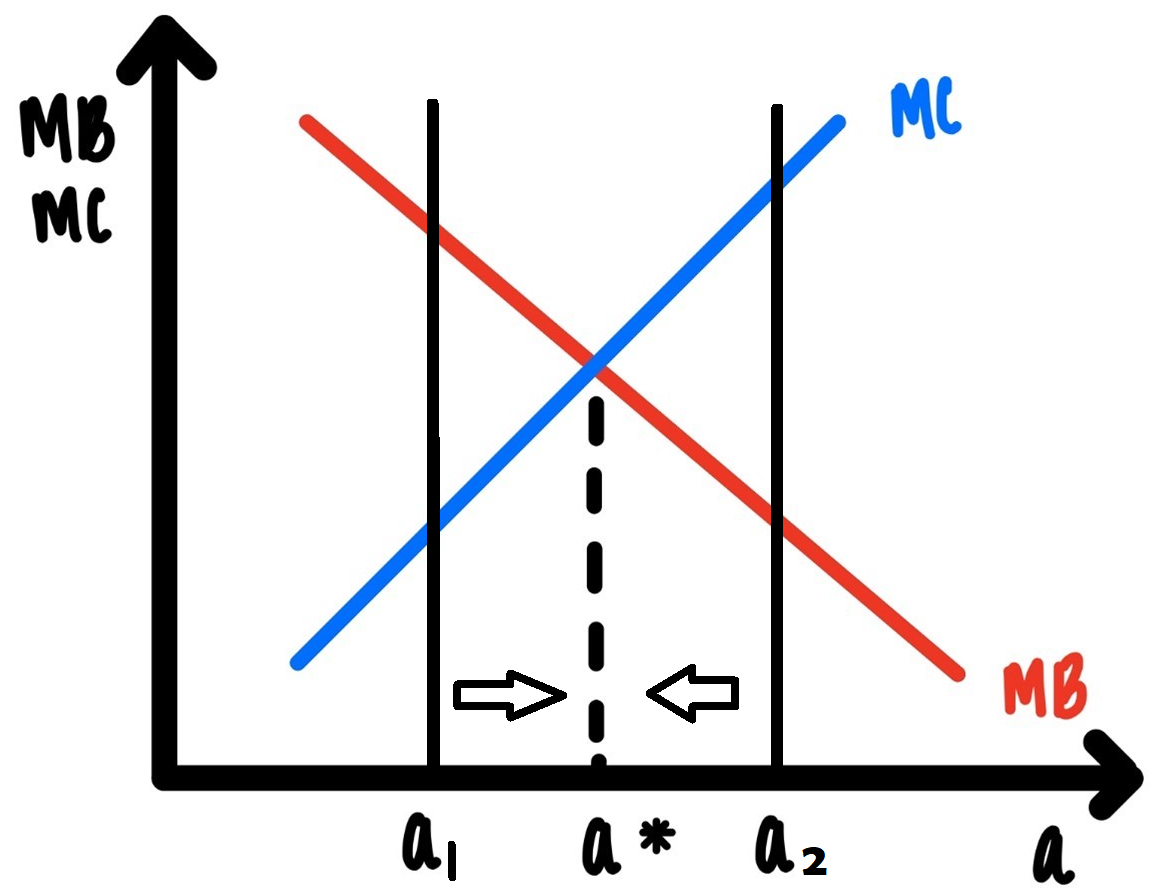
\includegraphics[width=0.75\linewidth]{img/rationalchoice/fig2} 

}

\caption{Rational Choice,}\label{fig:rationalchoice02}
\end{figure}

In Figure \ref{fig:rationalchoice02}, the marginal benefit of the action, MB, is downward sloping in accordance with assumption 1. The marginal cost of the action, MC, is upward sloping in accordance with assumption 2.

Claim: The optimal amount of time Leslie should study for the chemistry exam, IF Leslie is rational, is given by a*.

Why? Imagine that Leslie did anything else. Imagine she studied less, only \(a_1\). At that point, the marginal benefit of studying an extra half hour exceeds the marginal cost. So, Leslie should study an extra half hour. She should study more. She should move from \(a_1\) to the right closer to a* as indicated by the arrow pointing right. If Leslie is rational, she will do just that.

Imagine Leslie studies more, say \(a_2\). At that point, the marginal cost of studying that last half hour exceeds the marginal benefit. Sleep deprivation does not usually translate in high exam scores. At \(a_2\) Leslie should decide to study less. She should move to the left, as indicated by the arrow pointing left. Rational Leslie will do just that.

We have established in the case of Leslie studying for her exam, but much more generally:

\begin{iucolor}
\textbf{Rational action requires that the marginal benefit of an action is equated to the marginal cost of an action.}

\end{iucolor}

This conclusion which is illustrated in Figure \ref{fig:rationalchoice02} above will provide the basis for about 80\% of the material in this class. Figure \ref{fig:rationalchoice02} will show up in this class, again and again, just in different contexts.

In Figure \ref{fig:rationalchoice02}, the marginal benefit curve is downward sloping, and the marginal cost is upward sloping. We will encounter three versions of Figure \ref{fig:rationalchoice02} in this course. They are just very slight variations of Figure \ref{fig:rationalchoice02}. These are depicted in Figure \ref{fig:rationalchoice03}. Panel a is just a reproduction of Figure \ref{fig:rationalchoice02}. In panel b, the marginal benefit curve is a horizontal line, and the marginal cost is upward sloping. In panel c, the marginal benefit is downward sloping, and the marginal cost is a horizontal line.

\begin{figure}

{\centering 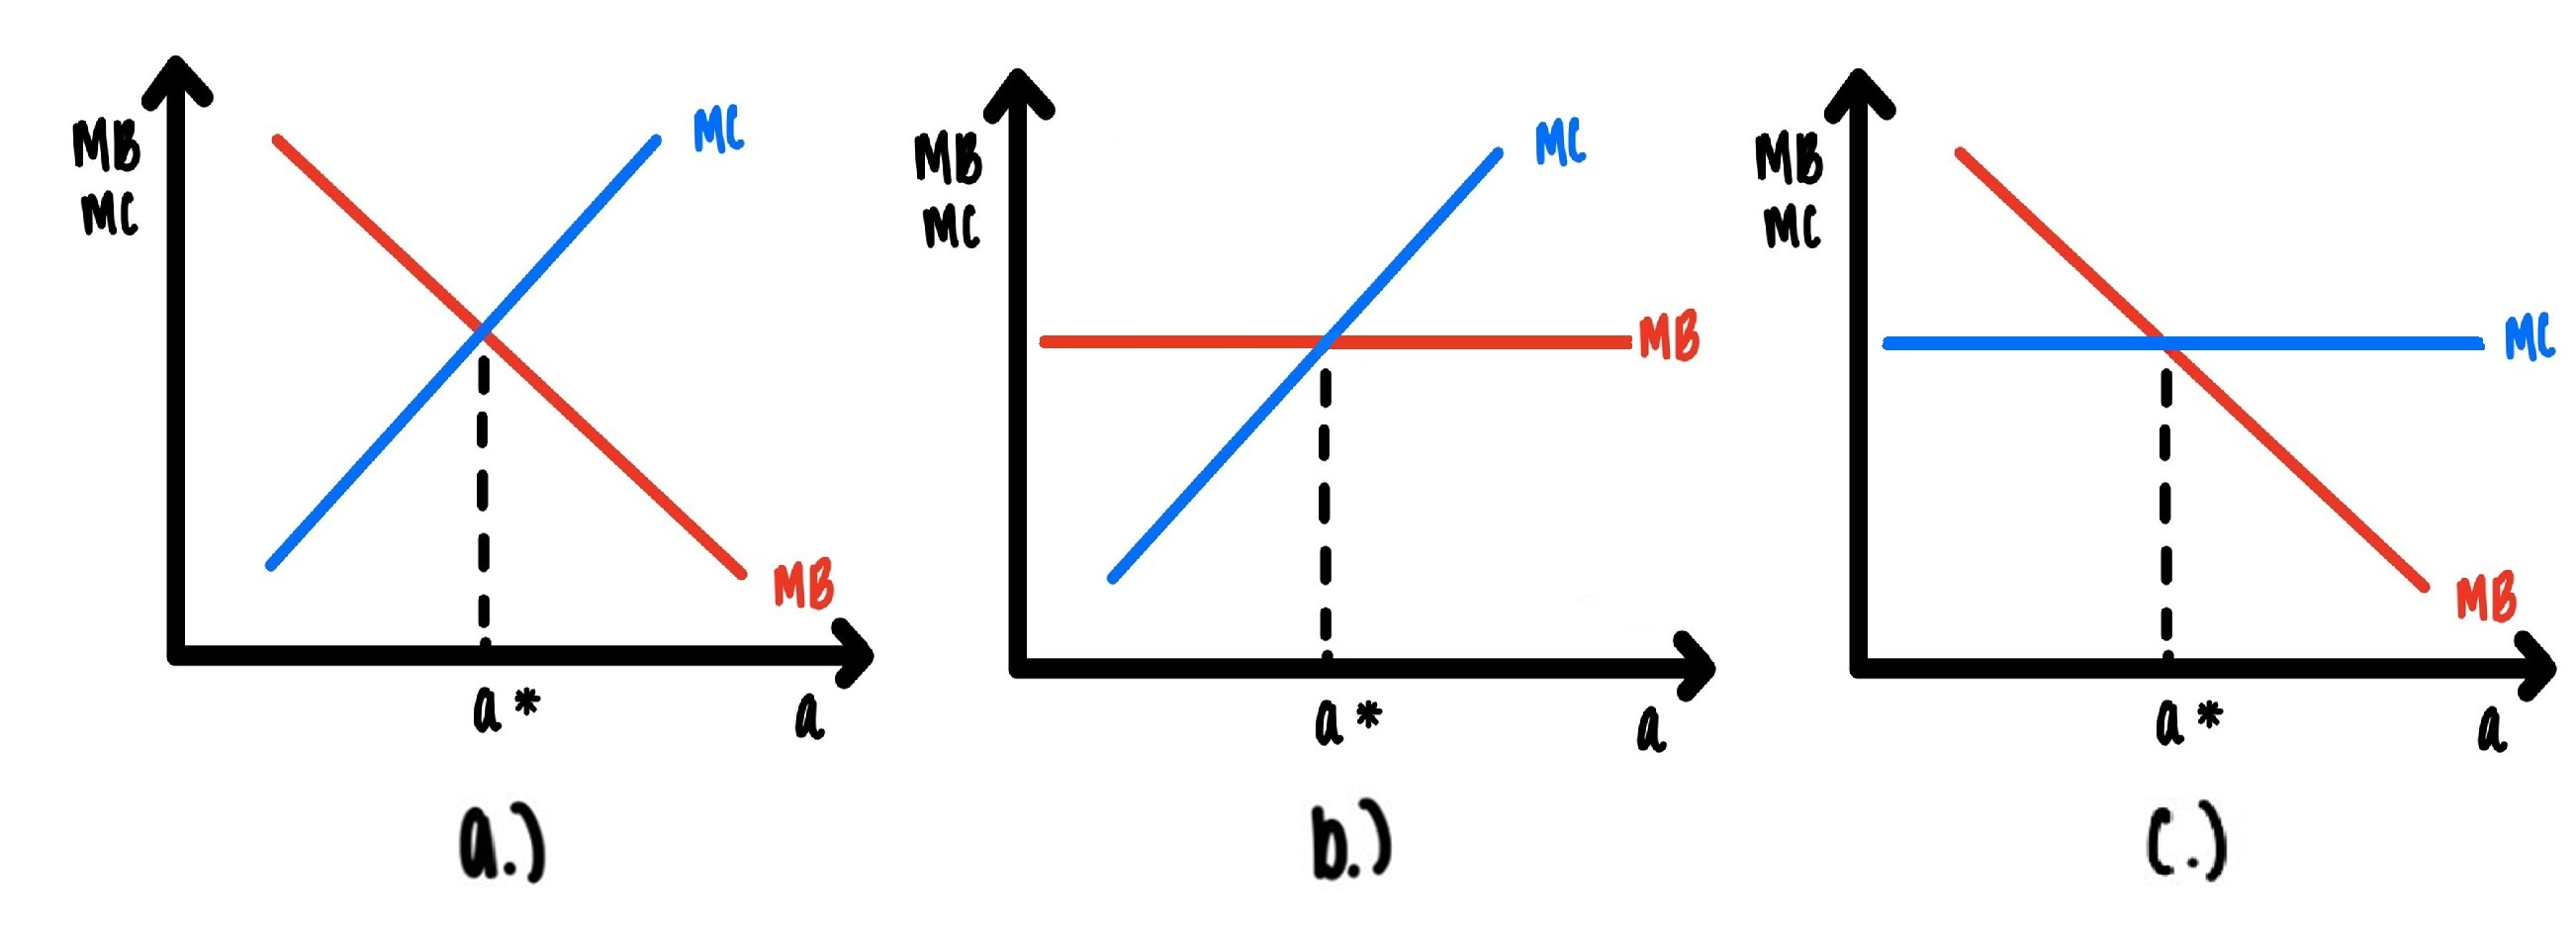
\includegraphics[width=1\linewidth]{img/rationalchoice/panels} 

}

\caption{This photo will reappear many times!}\label{fig:rationalchoice03}
\end{figure}

We can get from panel a to panel b by rotating the marginal benefit curve downward, so it becomes horizontal. We can get from panel a to panel c by rotating the marginal cost downward, so it becomes horizontal.

While these panels look slightly differently, they are just slightly different versions of the same thing:

At low levels of the activity, marginal benefit is above marginal cost. At high levels of the activity, marginal cost is above the marginal benefit. Somewhere in between there is a sweet spot, where marginal benefit equals marginal cost.

\hypertarget{changes-in-marginal-benefit-andor-marginal-cost}{%
\section{Changes in Marginal Benefit and/or Marginal Cost}\label{changes-in-marginal-benefit-andor-marginal-cost}}

What if some event occurs in which the marginal benefit or cost of an action changes?

The environment in which we live is not static. Our circumstances change all the time. In the framework laid out above there will be frequent changes in the marginal benefits and the marginal costs for our actions. How do these shifts influence rational action?

In Figure \ref{fig:rationalchoice04} we show how an increase in the marginal benefit of the action changes our rational choice.

\begin{figure}

{\centering 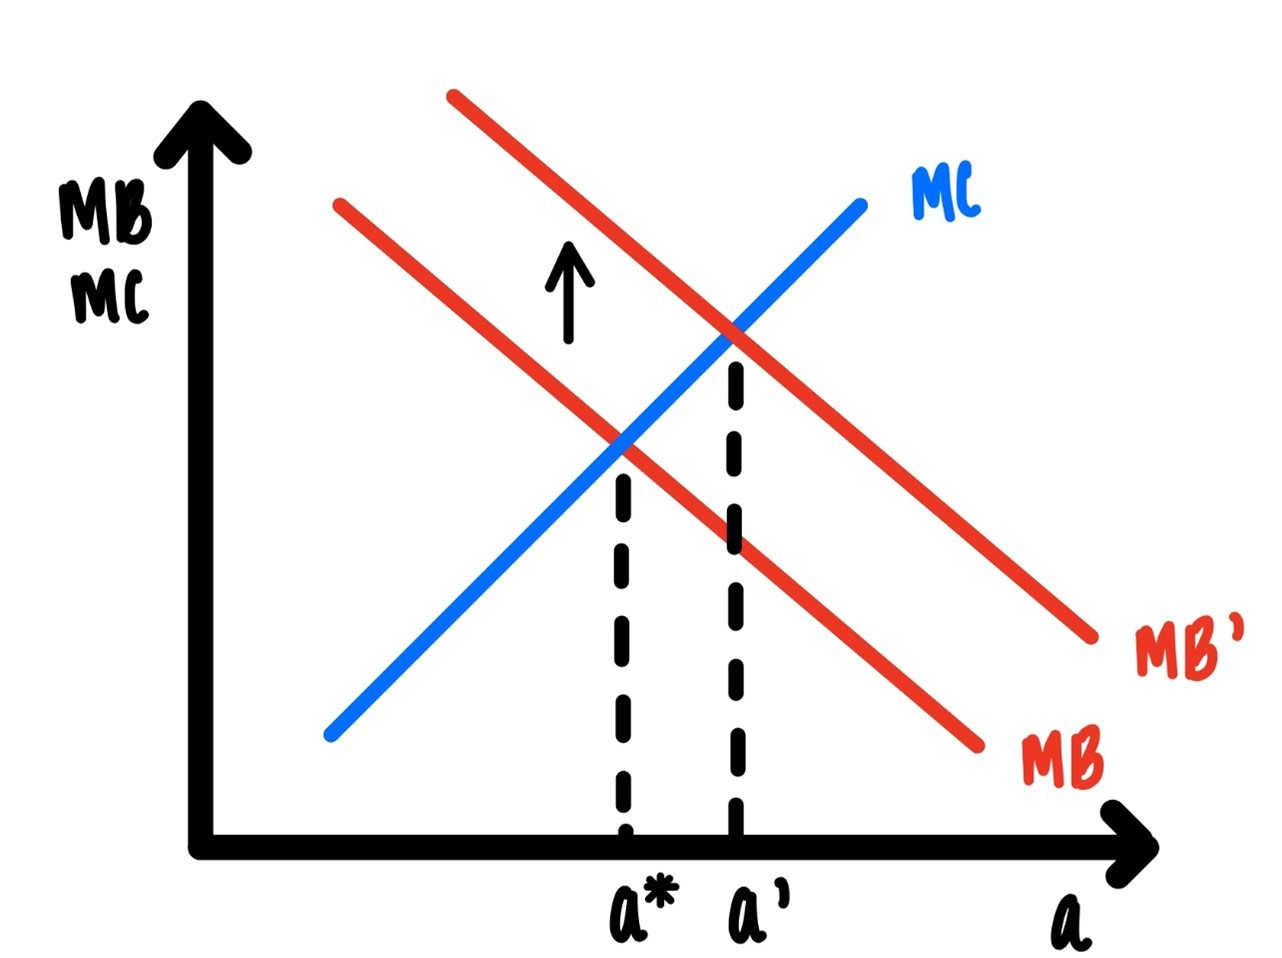
\includegraphics[width=0.75\linewidth]{img/rationalchoice/fig4} 

}

\caption{Increase of Marginal Benefit}\label{fig:rationalchoice04}
\end{figure}

Imagine that you are planning on a 3-hour hike by yourself this coming Saturday. Saturday morning your best friend calls you up and tells you he has nothing to do that day. You are overjoyed and invite him on the hike. Hiking with your best friend is much more enjoyable than a solitary hike. Because your friend accompanies you on your hike, the marginal benefit curve shifts out (Figure \ref{fig:rationalchoice04}) to the right. As a consequence, your 3-hour hike turns into a 4-hour hike. That is the rational response.

In Figure \ref{fig:rationalchoice05} we show how an increase in marginal cost of the action changes your rational choice.

\begin{figure}

{\centering 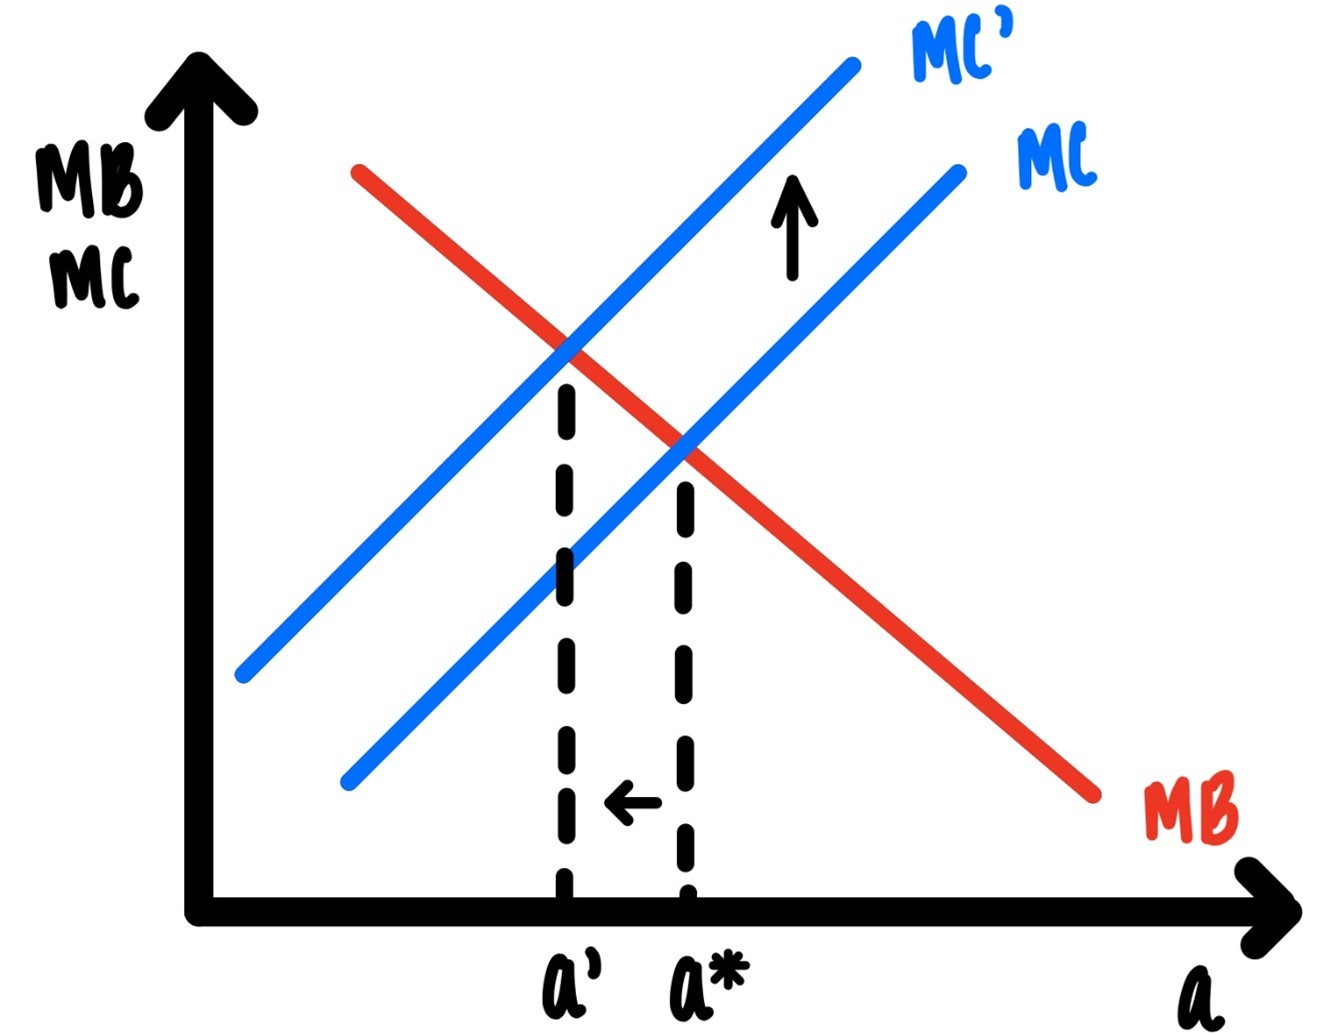
\includegraphics[width=0.75\linewidth]{img/rationalchoice/fig5} 

}

\caption{Increase of Marginal Cost}\label{fig:rationalchoice05}
\end{figure}

Imagine you are planning a 3-hour hike for this coming Saturday. Saturday morning your wake up and you realize that overnight there was torrential rain that turned the hiking trails in your area into mud. Each step is a muddy slog. Each step now is drudgery. The rain has increased the marginal cost of hiking (Figure \ref{fig:rationalchoice05}). Your 3-hour hike turns into a 2-hour hike. That is the rational response.

\begin{center}\rule{0.5\linewidth}{0.5pt}\end{center}

\hypertarget{examples-of-rational-choice}{%
\section{Examples of Rational Choice}\label{examples-of-rational-choice}}

\textbf{Example 3 (Refreshing Lemonade):} You just cut the grass on a hot July afternoon. You are hot, sweaty, and parched. Figure \ref{fig:rationalchoice06} captures the marginal benefit and the marginal cost of drinking lemonade. Assume the units of measurement are small glasses. The marginal cost of drinking lemonade is just the cost of each glass of lemonade. It is the same for each small glass. It is a horizontal line. The marginal benefit declines with each glass. The first glass is a great thirst quencher and so is, perhaps the second glass. Glasses three and four less so. By the sixth glass the marginal benefit is tiny, below marginal cost. It is rational for you to drink 4 glasses.

\begin{figure}

{\centering 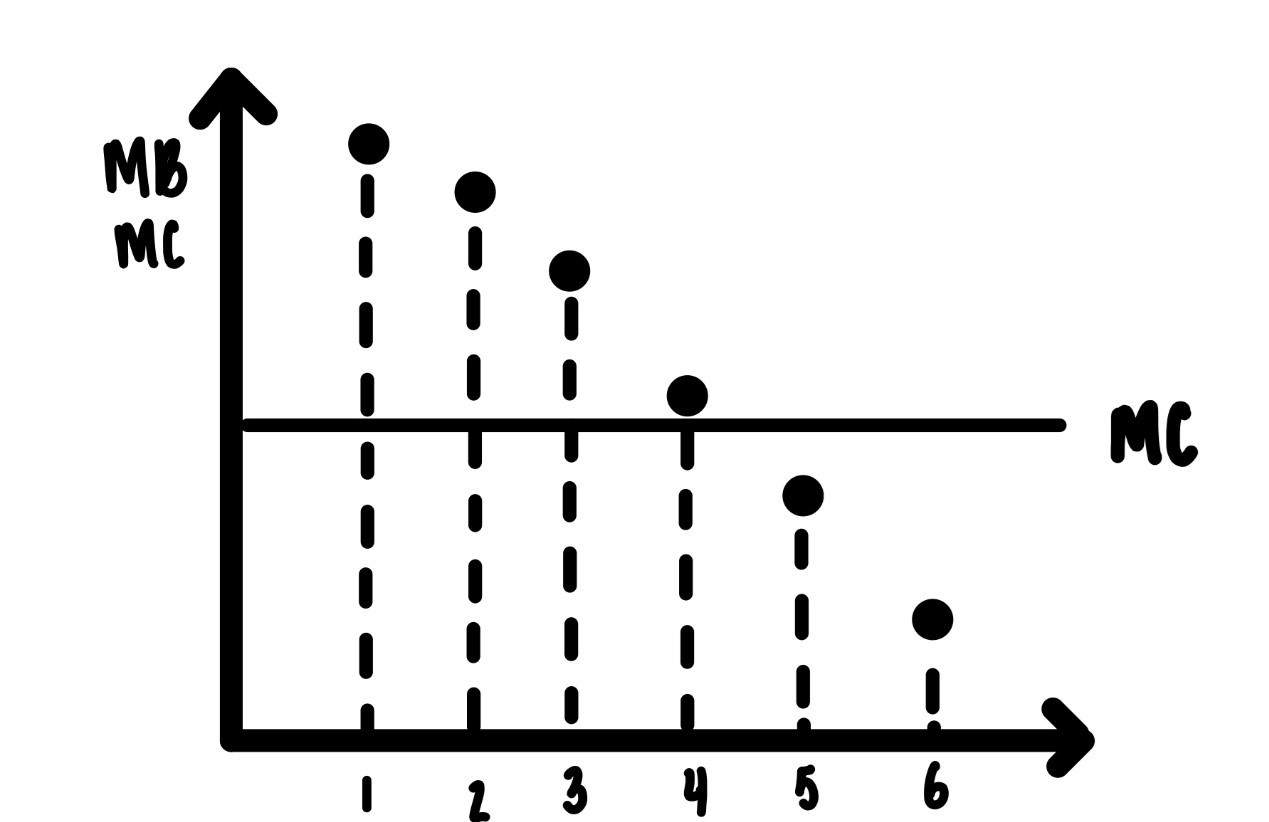
\includegraphics[width=0.75\linewidth]{img/rationalchoice/fig6} 

}

\caption{Drinking lemonade on a hot Saturday afternoon after you cut the grass.}\label{fig:rationalchoice06}
\end{figure}

\begin{center}\rule{0.5\linewidth}{0.5pt}\end{center}

\textbf{Example 4 (Optimal Retirement):} Joe is a dedicated high school math teacher. He has been teaching for 38 years and he has been planning to teach until his 70th birthday. After careful consideration of the joys of teaching, the marginal benefit, and the costs, this was his optimal choice. He has noticed that in the last few years, it has become harder to get up with a spring in his step every morning, and it has become harder to concentrate while grading papers. Yet, he still likes his job, with the joys outweighing any negative considerations. Then Covid-19 hit. Online teaching, lack of resources, concern for his health, administrative back and forth, administrative indecision, and opinionated parents who seem to stand in the way of effective teaching. This has caused his marginal benefit to shift way down. Now, retirement at age 67 instead of age 70 looks very appealing, and rational. \href{https://www.npr.org/2020/11/18/936096303/nurses-are-under-pressure-as-hospitals-strain-to-meet-pandemic-demands}{It appears, nurses are in the same storm.}

\begin{figure}

{\centering \includegraphics[width=0.75\linewidth]{img/rationalchoice/fig7} 

}

\caption{Optimal retiring age.}\label{fig:rationalchoice07}
\end{figure}

\begin{center}\rule{0.5\linewidth}{0.5pt}\end{center}

\textbf{Example 5 (Optimal Family Size):} What is our optimal number of kids? I know the number of children is not a continuous variable like how long to hike or how long to study for an exam. We still can imagine that there is a marginal benefit from having children and a marginal cost. Let's assume for the sake of simplicity that the marginal cost of a child is constant. I know that things like hand me down clothes might make the second child cheaper than the first, but this will not matter for the argument here. I also know that some parents look forward to having several children, rather than just one to see their children play with each other and grow up with each other. One could make therefore an argument that the marginal benefit of the second child might be higher than the marginal benefit from child number 1. Again, this would not influence the argument here. The point is that eventually the marginal cost of an extra child is higher than the marginal benefit of that child.
One interesting fact about desired fertility in the US seems to be: Whatever the number of children, if there is no boy among these children, the probability of having another child goes up. Suppose that for child 3, the marginal benefit is just above the marginal cost. Then the optimal rational number of children is 3. But things don't stop here. The sex composition of children seems to matter for the decision to have another child. If all three previous children are girls, indicated by the string (G, G, G), then the marginal benefit of having a fourth child is high, above marginal cost and the family has a fourth child. If there is at least one boy among the first three, indicated by the potential strings (B, G, G), (G, B, G), (G, G, B), (B,B, G), (G, B, B), then the marginal benefit of a fourth child is low. The family will only have three children.

That's the theory. That is also in the data. \url{https://econweb.ucsd.edu/~gdahl/papers/demand-for-sons.pdf}\\
American families tend to have a preference for sons over daughters.

\begin{figure}

{\centering \includegraphics[width=0.5\linewidth]{img/rationalchoice/fig8} 

}

\caption{Optimal fertility}\label{fig:rationalchoice08}
\end{figure}

\hypertarget{increasing-returns}{%
\section{Increasing Returns}\label{increasing-returns}}

We said earlier that diminishing returns is not an iron law. It is an assumption that is helpful in many cases. We have seen some examples above. There are cases where there are not diminishing but increasing returns.

\begin{center}\rule{0.5\linewidth}{0.5pt}\end{center}

\textbf{Example 6:} Suppose you want to build a bridge over the Mississippi just north of St.~Louis. It will require a ton of concrete. The point of the bridge is to get more transportation services from IL to MO and back. The marginal cost of the concrete can be assumed to be constant as seen in Figure \ref{fig:rationalchoice09}.

\begin{figure}

{\centering \includegraphics[width=0.75\linewidth]{img/rationalchoice/fig9} 

}

\caption{Concrete for bridge}\label{fig:rationalchoice09}
\end{figure}

The marginal benefit derived from the concrete is the shape of an inverted L. It is basically zero for practically every ton of concrete. There will be no transportation services at all until the very last ton of concrete is used to complete the bridge. Only when the last ton of concrete is laid, will there be any transportation services. Hence the inverted L shape.

\begin{center}\rule{0.5\linewidth}{0.5pt}\end{center}

\textbf{Example 7:} Suppose a widow, mother of two young children, is \(\$750\) behind on utilities. If she cannot pay the utility bill by next week, the power company will disconnect her service. Apart from not being able to heat the apartment and cook, disconnect from the power company means loss of her Section 8 housing and she and her two children will be homeless. Joe is a generous soul and gives her \(\$200\). That helps just a little bit, but her utility will still be shut off and she still faces the prospect of homelessness with her kids. Generous Jill pitches in another \(\$200\), and so does generous Jacqui. The marginal benefit of each one of these contributions is relatively small, since even with \(\$600\) she still faces the prospect of homelessness. Generous Jack finally pitches in another \(\$200\). This helps her over the top. It might be reasonable to assume that the marginal benefit to the widow of these contributions is as indicated in Figure \ref{fig:rationalchoice10}, convex at first, below the \$750 threshold and concave on the other side.

\begin{figure}

{\centering \includegraphics[width=0.75\linewidth]{img/rationalchoice/fig10} 

}

\caption{Benefit to widow of charitable contributions}\label{fig:rationalchoice10}
\end{figure}

\begin{center}\rule{0.5\linewidth}{0.5pt}\end{center}

\textbf{Example 8:} Why do you go to school? When I ask students that question the answer is invariably: To get a better job. And when I ask: What is a better job? the answer very often is something like: More money. The connection between schooling, years of schooling, and wages or earnings is one of the age-old central topics in labor economics.\footnote{\url{https://en.wikipedia.org/wiki/Mincer_earnings_function}}

\begin{figure}

{\centering \includegraphics[width=1\linewidth]{img/rationalchoice/fig11} 

}

\caption{Source: Cecilia Elena Rouse, 2017, The economics of education and policy: Ideas for a principles course, The Journal of Economic education, 48:3, 229-237}\label{fig:rationalchoice11}
\end{figure}

The return to an extra year of schooling is basically zero between 1 and 11 years of schooling. If you are in high school and contemplating whether you want to drop out after 9th grade or whether you want to stick it out for one more year, the data seem to indicate that the monetary return to the 10th year is zero. If you are in it for the money, it is better to finish high school.

After high school, earning rise linearly with each extra year of schooling. Even past 16 years of schooling. So, you may want to make the effort to really finish college and perhaps even get a graduate degree. Good luck with that!

\hypertarget{irrationality}{%
\section{Irrationality}\label{irrationality}}

In the examples we have studies so far, we have always assumed that individuals make rational choices. Rationality means doing one's best to attain one's goal or goals, given the information we have and staying within our constraints.

There is quite a bit of evidence that not all decisions are rational. Many of the examples of irrational behavior involve a time dimension of either costs or benefits of the decision. Most of us have been there and have seen some indication of what irrational behavior might be: New Year's rolls around and we resolve to start jogging and lose 20 pounds. But by March we have not jogged a mile, have not set foot in a gym, and forget about losing the 20 pounds. From eating all the chocolate, we have gained weight, not lost it.

Sometimes we just want to get one small snack, like one small piece of that delicious Swiss chocolate. So, we get the chocolate bar, break off one small piece, which is after all, all we want. But before we know it, the entire bar is devoured. And then regret sets in right away: Why did I eat so much chocolate? Why was I so stupid to eat the whole bar?

\hypertarget{sunk-costs}{%
\subsection{Sunk Costs}\label{sunk-costs}}

You get tickets for a Drake concert at the end of the month. You shell over the \$200 for the tickets. The morning of the concert, your girlfriend whom you love above all else, surprises you with a text message. She informs you that she finished her studies abroad at the London School of Economics early, that she is back in town and that she can't wait to spend the evening with you. You have missed her so much. Just the day before, before you saw the text, you told your body you would spend a thousand bucks to be with her. It is now too late to try to sell the Drake tickets on the secondary market.

What should you do? Most textbooks would say: You value the evening with your girlfriend more than going to the concert. The 200 bucks are sunk, they are a sunk cost. There is nothing you can do to retrieve the 200 bucks. Let

\begin{center}
``Bygones be bygones'',

\end{center}

forget about the cost of the tickets and enjoy the evening with your girlfriend.
Most econ text tell stories like that, give examples like that and then conclude that if you let sunk costs decide your behavior that you are engaged in what they call the

\begin{center}
Sunk cost fallacy.

\end{center}

The Sunk cost fallacy says: You are not acting rationally of you let the size of the sunk costs, irretrievable costs incurred in the past, influence your current behavior.

But if that is all they say, their analysis is at least incomplete.

Letting sunk costs influence our current behavior might actually be quite rational. In the first counter example we will see that financial constraints will making a difference here.

Consider a firm with a budget of \(B\) dollars. The firm is engaged in an investment project that has a rate of return of \(R_1\). That project requires a fixed cost of \(M_0\) dollars. The firm is making payments on this project in some increments over time. At some point, after having made some payments in the amount \(M_1\) on project 1, the firm discovers a new project that is better in the sense that it has a higher rate of return \(R_2 > R_1\). The new project has the same fixed costs \(M_0\).

If \(M_1 < M_0\), then the firm rationally switches to project 2 if and only if

\begin{center}
\((B – M_0) R_1 < (B – M_0 – M_1) R_2\)

\end{center}

It is easy to see that it is rational for the firm to switch to project 2 when B is large. But when B is small, i.e., when the firm faces a financial constraint, it will be rational for the firm to stay with the first project, EVEN THOUGH THE SECOND PROJECT IS BETTER.

Here is a more concrete example:

\begin{center}
``\ldots an aircraft company that had started a project to develop a radar-blank bomber plane might seem overly reluctant to switch to developing a radar-blank fighter plane if stealth fighters are suddenly in much greater demand; but their reluctance might be rational because they might have a limited budget, might have already spent hundreds of millions of dollars on developing a cost-effective bomber, and would have to pay another large fixed cost to develop a cost-effective fighter instead.''

\end{center}

So much for the sunk cost fallacy in this context. It is rational to ``throw good money after bad money''.

The sunk cost fallacy may fall apart for other reasons as well. Some of these have to do with information and reputation.

Consider a manager who chooses a project. The manager is acting as the agent for the stockholders, the principals. Of course, the stockholders do not have perfect information about the quality, the ability of the manager. They infer ability of the agent from actions and outcomes.

While the project is being carried out, the manager acquires some information about the project. That information is typically private to the manager; the stockholders do not have access to the information. How are projects chosen? Hard to say, but it stands to reason that high ability managers choose high return projects more frequently than low ability managers might.

If a manager abandons a project, stockholders, the principal, might draw negative inferences about the manager's ability. The manager of course has an interest in avoiding such an inference because that would negatively impact future earnings potential. For this reason, it is often rational for a manager to continue funding an unproductive project. Letting ``bygones be bygones'' may not be rational for him. The simple version of the sunk cost fallacy does not apply here. Even if the project is ultimately declared a failure with the manager being fired because of that failure, delaying that firing as long as possible may well be the most rational thing for the manager to do.

So much for the sunk cost fallacy in this context. It is rational to ``throw good money after bad money''.
The problem of rationally throwing good money after bad money may even be intensified in the political context. If I know there is a good chance that I will not be re-elected at the next election in two or four or six years, then, if I know the current project has turned out to be a lemon, I have a very large incentive of throwing good money after bad, so that the outcome of my bad decisions can be blamed not on me, but on my successor.

\hypertarget{examples-2}{%
\subsection{Examples}\label{examples-2}}

\textbf{Example 9 (Gym membership, we don't sweat it, but perhaps we should.):}\footnote{
  \url{https://pubs.aeaweb.org/doi/pdfplus/10.1257/aer.96.3.694}}

Gym member ship typically comes in three varieties: annual memberships, monthly memberships and daily passes. Prices in the sample in the paper above are approximately \$12 per day, between about \$85 per month for the monthly membership, and about \$850 for an annual pass. Typically, you sign up for one of these options and then, after you signed one of these contracts, you go to the gym.

Or not.

That is exactly the issue studied in \href{https://pubs.aeaweb.org/doi/pdfplus/10.1257/aer.96.3.694}{this paper by Stefano DellaVigna and Ulrike Malmenidier}.

How would we think of rationality in this context? Rationality here implies that the choice of contract is consistent with actual exercise behavior. Signing up for a monthly contract is in your best interest if you actually go to the gym more than 7 times a month. (7 times 12 is 84) If you go to the gym fewer than 7 times a month, the daily memberships would have been a better deal. Similar comparisons can be made to decide on the rationality of choosing between the monthly and the annual contracts.

Here is what the authors find in their sample of over 7,700 individuals:

\begin{enumerate}
\def\labelenumi{\arabic{enumi}.}
\item
  Those who choose a monthly contract pay on average 70\% more relative to the daily contracts. How can this happen? Go 4 times a month. Using the daily passes costs \$48. The monthly pass costs \$85. (85-48)/48 = 37/48 = 77\%.
\item
  The number of people overpaying like this is large. 80\% of all customers would have been better off with the daily passes rather than the monthly contract.
\item
  Consumers who use the monthly contracts are 17\% more likely to stay beyond one year than users of the annual contracts, even though using the monthly contract is more expensive in that case.
\end{enumerate}

What is going on? It appears that most customers are naïve and over-estimate their future self-control. Looks like rationality has gone out the window.

These kinds of irrational behaviors often happen when there is a time or temporal element involved, which surely is the case in the choice of picking gym membership contracts.

Choose the contract today, and exercise in the future. Or not.

This is similar in many ways to:

\begin{itemize}
\item
  Trip to the Dairy Queen today and the expectation of starting a jogging regimen in the future. But then the jogging does not happen. The benefits of the ice cream are today, the costs come in the future. And with the costs might come regrets. Why did I have that ice-cream?
\item
  The pleasure of smoking today and lung cancer at age 62. Regrets?
\item
  The costs of going to college today and the benefits of higher earnings over the entire productive life. Are there any regrets of not having worked hard enough in college?
\item
  Hooking up and enjoying the pleasure of sex tonight. The pleasure comes tonight, the potential costs in the future. The regret may set in already the following morning. The STDs may set in later and last a long time. By some estimates 1 in 2 people will contract a STI by age 25. The risk of getting infected during a hook up is substantial. 14\% of male college students report 4 or more sexual partners in the last 12 months. For women in college that number is 9\%. In a hookup, who is your partner? What is the risk? The three quarters of college students who report zero or one sexual partner probably present a smaller risk of infection, but they are probably not involved in the hook up culture. So how big is the risk? How likely is regret? \footnote{
    \url{https://scivisionpub.com/pdfs/sexually-transmitted-infections-among-college-students-1481.pdf}
    \url{https://enagoski.medium.com/}} \footnote{these-graphs-tell-a-shocking-story-about-the-rampant-college-hookup-culture-38a0ef1b0af8}
\end{itemize}

\hypertarget{glossary-of-terms-3}{%
\section{Glossary of Terms}\label{glossary-of-terms-3}}

\textbf{Diminishing returns:} In production, the amount of extra output produced by an extra unit of an input declines as more of the input is used. Or, alternatively, as the amount of an input used is increasing, it requires more and more of that input to produce one extra unit of output.

\textbf{Diminishing utility:} In consumption, the amount of extra utility/satisfaction/pleasure generated by an extra unit of the consumption good declines as more and more of that good is consumed.

\textbf{Increasing returns:} In production, the amount of extra output produced by an extra unit of input increases as more of the input is used. Or, alternatively, as the amount of an input used in production is increasing, it requires less and less of the input to produce one extra unit of the output.

\textbf{Increasing utility:} In consumption, the amount of extra utility/satisfaction/pleasure generated by an extra unit of the consumption good increases as more and more of the good is consumed.

\textbf{Marginal benefit:} The marginal benefit of any action is the extra benefit derived from one additional unit of the action.

\textbf{Marginal cost:} The marginal cost of any action is the extra cost incurred to carry out that action by one more unit.

\textbf{Opportunity cost:} The opportunity cost of any action is the value that could have been obtained from the second-best available option, had the second-best option been chosen.

\textbf{Rationality/rational choice:} Choosing an option within the constraints or limits that gets the decision maker closest to their goal, where the decision maker is using all the available information.

\hypertarget{practice-questions-3}{%
\section{Practice Questions}\label{practice-questions-3}}

\hypertarget{discussion-3}{%
\subsection{Discussion}\label{discussion-3}}

\begin{enumerate}
\def\labelenumi{\arabic{enumi}.}
\item
  In your own words describe how economists use the term ``rationality''.
\item
  Provide two examples of activities where the marginal benefits are rising as the activity is increased.
\item
  Provide two examples of activities where the marginal costs are falling as the activity is increased.
\item
  Suppose you care only about two goods, food and clothing. We denote the amounts of food and clothing by f and c, respectively. We denote your income, monthly, while on campus in the fall semester by m. The two prices are \(p_f\) and \(p_c\), respectively.

  A. Write down an equation that captures your budget constraint.\\
  B. Your parents call you up in August right after you arrived on campus and tell you that your monthly income for the rest of the semester has increased by 15\%. How, in percentage terms, would your monthly expenditures on food and clothing change?\\
  C. What if your monthly income changed only for the month of September.
\item
  Before you arrive on campus you have heard all kind of horror stories about ``Finite Math.'' Against all odds, you discover in the first two weeks of class that you actually really, really like it. Illustrate with an appropriate graph how this discovery might influence how much time you might allocate to study ``Finite''.
\item
  Describe three examples of increasing returns in consumption. Why do the increasing returns arise?
\item
  Describe three examples of increasing returns in production. Why do the increasing returns arise?
\end{enumerate}

\hypertarget{multiple-choice-3}{%
\subsection{Multiple Choice}\label{multiple-choice-3}}

\begin{enumerate}
\def\labelenumi{\arabic{enumi}.}
\item
  Jack likes to go out and have pizza with his buddies. He always looks forward to that first slice. The second slice usually is a tad less enjoyable than the first. By the fourth slice, most of the thrill of eating pizza is gone. This is an example of

  A. Opportunity cost\\
  B. Rational choice\\
  C. Increasing returns\\
  D. Decreasing returns
\item
  Jill purchases her eggs for breakfast directly from Farmer Brown. Farmer Brown sells free roam, no pesticide, organic eggs. Starting October 1, Farmer brown changed this and as a consequence the eggs no longer taste like eggs Jill used to love. As a consequence of this change, Jill's

  A. Marginal cost of eating eggs shifts up\\
  B. Marginal cost of eating eggs shifts down\\
  C. Marginal benefit from eating eggs shifts up\\
  D. Marginal benefit from eating eggs shifts down
\item
  Your favorite breakfast cereal gets improved, and you find it tastes much better. This change will

  A. Make your marginal benefit from cereal flatter\\
  B. Make your marginal benefit from cereal steeper\\
  C. Shift your marginal benefit from cereal up\\
  D. Shift your marginal benefit from cereal down
\item
  You discover a better charcoal that makes the burgers you grill taste better. As a consequence of having discovered the better charcoal, your

  A. Marginal cost of burgers has increased\\
  B. Marginal cost of burgers has decreased\\
  C. Marginal benefit from burgers has decreased\\
  D. Marginal benefit from burgers has increased
\item
  ``Diminishing marginal returns'' is

  A. A fact\\
  B. An assumption\\
  C. True\\
  D. False
\item
  ``Increasing returns'' is a situation where

  A. Marginal costs are upward sloping\\
  B. Marginal costs are downward sloping\\
  C. Marginal costs are above marginal benefit\\
  D. Marginal costs are below marginal benefit.
\item
  Suppose Jack owns 8 pairs of shoes. At 8 pairs of shoes her marginal benefit from one extra pair of shoes is \(\$300\). The marginal cost of an extra pair of shoes is \(\$200\). Then rationally

  A. Jack should buy more shoes\\
  B. Jack should buy fewer shoes\\
  C. Jack has purchased the optimal (for Jack) number of shoes\\
  D. Jack should go barefoot.
\item
  Gerhard wants to be a rockstar and play the electric guitar. His marginal benefit of practicing the guitar is always/everywhere above the marginal cost of practicing, whatever that may be. Then, if Gerhard is rational,

  A. He should practice more\\
  B. He should practice less\\
  C. He should abandon his dream of becoming a rock star\\
  D. He should pick up jazz dance
\item
  The marginal benefit of saving is the extra consumption you can afford in the future. The marginal cost of saving is the consumption foregone today. Currently tax rates are at historic lows, and you are confident that tax rates will have to increase in the future. If taxes will indeed increase in the future, then

  A. The marginal benefit of saving decreases\\
  B. The marginal benefit of saving increases\\
  C. The marginal cost of saving increases\\
  D. The marginal cost of saving decreases
\item
  Jackie is very healthy and expects to remain healthy until she draws her last breath. Jack is expecting to develop all kinds of health problems as he ages. If these assessments are correct, then

  A. Jackie's marginal benefit of saving is higher than Jack's\\
  B. Jackie's marginal benefit of saving is lower than Jack's\\
  C. Jackie's marginal cost of saving is higher than Jack's\\
  D. Jackie's marginal cost of saving is lower than Jack's
\item
  Rudolf's marginal benefit from pulling a sleigh through the snow and ice is exactly equal to Rudolph's marginal cost of pulling the sleigh. If Rudolph is rational, Rudolph should

  A. Pull more\\
  B. Pull less\\
  C. Not change the amount of pulling\\
  D. Put more gifts on the sleigh
\item
  Mary is planning to go out for dinner Friday night. Before she goes out, she makes a list of the preferences over meals. Mary prefers lobster over chicken, chicken over a burger, a burger over pizza, pizza over mixed vegetables. When she gets to the restaurants, she finds out that the lobster is not available. She chooses the chicken. Her opportunity cost of choosing the chicken is the value she would have obtained from

  A. Lobster\\
  B. Mixed vegetables\\
  C. Pizza\\
  D. The burger
\item
  In the above problem the highest amount Mary is willing to pay for lobster, chicken, burger, pizza, mixed vegetables are in dollars, 35, 30, 25, 20, 15. The prices of these goods, in the same order are, also in dollars, 30, 25, 20, 15, 10. If the price of mixed vegetables rises to 12 dollars, then Mary's opportunity cost of eating chicken

  A. Rises\\
  B. Falls\\
  C. Stays constant\\
  D. Is irrelevant for her decision
\item
  In the above problem with the original valuations by Mary and the original prices, when Mary arrives at the restaurant, she finds out that the only burger available is a bison burger, not the Angus beef that she usually prefers. In this case her opportunity cost of eating chicken has

  A. Increased\\
  B. Decreased\\
  C. Stayed constant\\
  D. Become irrelevant
\item
  Jack is moving into a new apartment. He cannot lift a heavy sleeper sofa by himself. When Jill arrives, the two of them together can move the sleeper sofa into the new apartment. This is an example of

  A. Opportunity costs\\
  B. Diminishing returns\\
  C. Increasing returns\\
  D. Rationality
\item
  Mary and Jill both like doing housework equally well. Mary has a degree in Finance from IU, Jill dropped out of high school after 11th grade. If both Mary and Jill are rational, then

  A. Mary will allocate more hours to housework than Jill\\
  B. Mary will allocate fewer hours to housework than Jill\\
  C. Mary and Jill will spend the same number of hours doing housework\\
  D. Jill will hire a nanny.
\item
  When Mary gets a raise her

  A. Marginal cost of housework increases\\
  B. Marginal cost of housework decreases\\
  C. Marginal benefit of housework increases\\
  D. Marginal benefit of housework decreases
\item
  Beckie loves drinking coffee with a good amount of hazelnut flavored coffee creamer. If that kind of coffee creamer is unavailable

  A. Her marginal cost of coffee rises\\
  B. Her marginal cost of coffee falls\\
  C. Her marginal benefit of coffee rises\\
  D. Her marginal benefit of coffee falls
\item
  Rationality means

  A. Choosing a level of activity where marginal benefit is highest\\
  B. Choosing a level of activity where marginal cost is lowest\\
  C. Choosing a level of activity where marginal cost is far below marginal benefit\\
  D. Choosing a level of activity where marginal benefit is equal to marginal cost
\item
  You are playing center mid on your intra mural soccer team. At the beginning of the season, your teammates always played their hearts out and your team won quite a few games. In today's game you realize that your teammates don't want to run, they don't seem to have their heart in the game. As a consequence

  A. Your marginal cost of playing hard rises\\
  B. Your marginal cost of playing hard falls\\
  C. Your marginal benefit of playing hard rises\\
  D. Your marginal benefit of playing hard falls
\end{enumerate}

\hypertarget{answer-key-2}{%
\subsection{Answer Key}\label{answer-key-2}}

\begin{enumerate}
\def\labelenumi{\arabic{enumi}.}
\tightlist
\item
  D
\item
  D
\item
  C
\item
  D
\item
  B
\item
  B
\item
  A
\item
  A
\item
  A
\item
  A
\item
  C
\item
  D
\item
  C
\item
  B
\item
  C
\item
  B
\item
  A
\item
  D
\item
  D
\item
  D
\end{enumerate}

\hypertarget{demand}{%
\chapter{Demand}\label{demand}}

In this chapter we will learn:

\begin{itemize}
\tightlist
\item
  How the demand curve is constructed from the marginal benefit curve
\item
  The law of demand
\item
  How to derive market demand from individual demands\\
\item
  The factors that shift demand
\item
  The notion of the elasticity of demand
\end{itemize}

\hypertarget{introductory-video}{%
\section{Introductory Video}\label{introductory-video}}

\url{https://iu.mediaspace.kaltura.com/media/t/1_6qqdrvui}

\hypertarget{what-is-demand}{%
\section{What is Demand?}\label{what-is-demand}}

In this chapter, we will study one of the central ingredients used to analyze markets. In this chapter, we will study demand.

Many people throw around the term ``demand'' and they talk about ``supply and demand'' without apparently having full comprehension and understanding of these terms. The term demand has a very particular meaning, and we will begin by illustrating this meaning.

We go back to a figure in the previous chapter. There we studied the rational choice of drinking lemonade or iced tea after mowing the lawn on a hot July afternoon. In this figure, the marginal benefit of drinking an extra glass of lemonade was downward sloping. That is just the assumption of diminishing returns to the lemonade. In this picture the marginal cost of lemonade was simply the price of an extra glass of lemonade.

\begin{figure}

{\centering \includegraphics[width=0.5\linewidth]{img/rationalchoice/fig6} 

}

\caption{Drinking lemonade on a hot Saturday afternoon after you cut the grass.}\label{fig:demand01}
\end{figure}

The rational choice for lemonade consumption was exactly at the intersection of marginal benefit from the lemonade and the marginal cost of lemonade, which is, of course, the price of lemonade. This is exactly the punchline from this figure in our chapter on Rational Choice.

\begin{figure}

{\centering \includegraphics[width=0.75\linewidth]{img/demand/fig2} 

}

\caption{Demand for Lemonade}\label{fig:demand02}
\end{figure}

In Figure \ref{fig:demand02}, here in this chapter, we show how that one consumer's, Joe's, rational choice of lemonade consumption changes with the price of lemonade. As the price of lemonade increases, it is rational to consume less lemonade. As the price of lemonade decreases, it is rational to consume more lemonade. In Figure \ref{fig:demand02} as the price of lemonade varies from \(p_1\) to \(p_2\) to \(p_3\), the rational choice of lemonade consumption varies from \(q_1\) to \(q_2\) to \(q_3\).

We can now state:

\begin{iucolor}
\textbf{The Law of Demand: When the price of a good increases (decreases), the quantity demanded decreases (increases).}

\end{iucolor}

As the price varies, Figure \ref{fig:demand02} tells us exactly how the rational choice of lemonade consumption varies. And this rational choice of lemonade consumption is determined by the marginal benefit derived from lemonade consumption. As the price of lemonade varies from a very low value to a very high value, we sweep out the entire marginal benefit curve. This allows us to say that:

\begin{iucolor}
\textbf{The marginal benefit curve IS the demand curve.}

\end{iucolor}

Or reversed, the demand curve of a product or service is the marginal benefit curve from that product or service.

Demand is the entire marginal benefit curve. Demand has to be distinguished from the quantity demanded. The quantity demanded is just one point on the demand curve. That is how much consumption is rationally chosen at a given price. Demand is the entire curve. We will always have to make this distinction.

What does demand represent? Demand represents the marginal benefit a consumer derives from a particular good. It is purely idiosyncratic. Jack's demand for lemonade will be different from Joe's and Joe's demand will be different from Jill's. That is what it is, and we will not quibble at all about what these preferences are and why they might differ.

Jack's demand for lemonade can, of course, change over time. It will be higher on a hot summer day than on a cold November day. It will be higher in the afternoon than in the morning. Over longer periods, Jack's preferences might also slowly shift away from lemonade, sweet and sugary, to low calorie iced tea or even water.

\hypertarget{individual-to-market-demand}{%
\subsection{Individual to Market Demand}\label{individual-to-market-demand}}

The analysis above involved demand from an individual consumer. How do we get from individual demand to market demand?

Easy. Just add up the individual demands. How this is done is illustrated in Figure \ref{fig:demand03} below for the simplest possible case of two consumers, called Joe and Mary. Joe's demand is in panel a, Mary's demand is in panel b.

\begin{figure}

{\centering \includegraphics[width=1\linewidth]{img/demand/fig3} 

}

\caption{Market Demand}\label{fig:demand03}
\end{figure}

Both Joe and Mary face the same price. If the price is \(p_1\), then Joe's quantity demanded is indicated by the distance ``\(a\)'' and Mary's quantity demanded is indicated by the distance ``\(b\)''. In panel c, these to distances are added together to get market quantity demanded to be ``\(a+b\)''. We can do this at any price, not just at \(p_1\), to obtain the entire market demand function as in panel c.

This can be done for any product and for any set of consumers.

\hypertarget{alternate-view-of-demand}{%
\subsection{Alternate View of Demand}\label{alternate-view-of-demand}}

There are many products or services that are not really divisible. Either you buy them, or you don't. Examples include large ticket items: a car, a washing machine, jet skis, or your dream vacation to Bora Bora or Glacier National Park.

Our typical view of demand is: At a particular price, how much stuff is sold? Here we go from the vertical axis, the price axis, over to demand and down to the horizontal axis, the quantity axis, and read off the quantity demanded.

We can turn this around and ask: For a particular good or service, what is the maximum amount a customer is willing to pay? Here we go from the horizontal axis, the quantity axis, up to demand and over the vertical axis, the price axis, to read off the maximum willingness to pay.

This maximum willingness to pay is sometimes called the reservation price. The reservation price is also that price which leaves the consumer just indifferent between buying or not buying.

Then, we can line up all the potential consumers in order of their reservation price, with the highest reservation prices on the left and the lowest reservation prices on the right. And, surprise, surprise, we get a downward sloping demand curve.

\hypertarget{elasticity}{%
\section{Elasticity}\label{elasticity}}

In the previous section we have established the Law of Demand, that demand is downward sloping, that an increase in the price causes a decrease in the quantity demanded. All of these statements say the same thing.

Here we will think about the slope of the demand function. Notice in Figure \ref{fig:demand03}, Joe's demand is a lot steeper than Mary's demand. What determines when a demand is steep or flat? The slope of the demand function will indicate how responsive consumers are to changes in the price. This is crucial information to have when a firm sets prices of products. Total revenue will depend upon this responsiveness.

Total revenue is always price time quantity. If p is the price and q is the quantity sold by a firm, the total revenue is given by

\[TR = p \times q(p)\]

There we expressly show that the quantity sold typically depends on the price: the demand function is downward sloping. The price going up is a good thing for revenue. But then, almost invariably, the quantity goes down. This is bad for revenue. One effect is good, the other effect is bad.

Which is bigger?

That is exactly where the concept of elasticity comes in. It is easy to see that if the price goes up say 10\% and the quantity goes down by 20\%, the bad outweighs the good and revenue will go down.

The moral of this story is:

Know thine elasticities!

We will use the concept of an elasticity, which we denote shorthand as \(\epsilon\). Here the price elasticity is defined as

\[\epsilon=\frac{\text{percentage in quantity demanded}}{\text{percentage change in price}}\]

This concept is relatively easily illustrated with a few examples.

\begin{enumerate}
\def\labelenumi{\arabic{enumi}.}
\tightlist
\item
  If the price changes by 10\% and the elasticity is 0.6, then the quantity demanded changes by 6\%.
\item
  If the price changes by 10\% and the quantity demanded changes by 7\%, then the elasticity of demand is 0.7.
\item
  If we know that the elasticity of demand is 0.5 and we see that that quantity demanded has changed by 15\%, then we can infer that the price has changed by 30\%.
\item
  If the price elasticity is bigger than one, a price increase will cause revenue to go down.
\item
  If the price elasticity is less than one, a price increase will cause revenue to go up.
\end{enumerate}

All of this involves very basic math. In the expression for the elasticity, there are three variables. If you know two of these, you can solve for the third. No magic required.

\begin{figure}

{\centering \includegraphics[width=1\linewidth]{img/demand/fig4} 

}

\caption{Differences in Elasticities}\label{fig:demand04}
\end{figure}

When the elasticity is low, the demand curve will be very steep as in panel a in Figure \ref{fig:demand04} . When the elasticity is high, the demand curve will be very flat as in panel b. We will speak of elastic demand when \(\epsilon\) is high and inelastic demand when \(\epsilon\) is low.

A few remarks:

\begin{enumerate}
\def\labelenumi{\arabic{enumi}.}
\item
  In the equation/definition of the elasticity above, the elasticity is negative: When the price changes, the quantity demanded goes in the opposite direction. Hence \(\epsilon\) in the above equation is negative. In what follows we will always take the absolute value of ϵ to indicate the elasticity. The elasticity will always be a positive number.
\item
  The elasticity of demand is not an immutable law. It will vary from product to product. It will vary from consumer to consumer. Even, for individual consumers, the elasticity can vary, depending on the price. All we have are estimates of these elasticities.
\item
  The time horizon matters. When prices change, consumers often adjust. The more time that is available for the adjustment, the larger the adjustment can be. In other words: the long-run elasticities will be larger than the short-run elasticities.
\end{enumerate}

Now suppose that your favorite soft drink is FSSW, Frizzy Sudsy Sugary Water and imagine that your favorite breakfast cereal is CCSB, Chocolate Covered Sugar Bombs, or is it SCCB, Sugar Covered Chocolate Bombs. Walking down the aisles in your favorite grocery store convinces you, see also Figure \ref{fig:demand05}, that there are lots and lots of substitutes for FSSW and for CCSB.

\begin{figure}

{\centering \includegraphics[width=0.45\linewidth]{img/demand/fig5} \includegraphics[width=0.45\linewidth]{img/demand/fig5b} 

}

\caption{Substitutes galore. Images sourced from unsplash.}\label{fig:demand05}
\end{figure}

As there are tons of substitutes a small increase in the price, may induce many consumers to switch to one of the many available substitutes. In this case we would expect the demand for the product to be very elastic.

On the other hand, there are some products that have few, if any, substitutes. Two of such products are shown in Figure \ref{fig:demand06}: coffee and toothpaste, not the particular brands, but coffee and toothpaste.

\begin{figure}

{\centering \includegraphics[width=0.45\linewidth]{img/demand/fig6} \includegraphics[width=0.45\linewidth]{img/demand/fig6b} 

}

\caption{Images sourced from unsplash.}\label{fig:demand06}
\end{figure}

Some people would argue that there are decent substitutes available for coffee, like black tea or caffeinated soft drinks. But what do they know? For many of us, neither tea nor soft drinks are anywhere near to being decent substitutes for coffee. So, we would expect the demand for coffee to be relatively inelastic.

The same for toothpaste. There are no substitutes for toothpaste. Even if the price of toothpaste were to double or triple, I would not brush my teeth any less. Most of us would not. Again, this points to inelastic demand.

We are not talking about particular brands of coffee or particular brands of toothpaste, but about coffee in general and toothpaste in general. There is one more aspect of toothpaste that especially helps explain why we would expect demand to be inelastic: It occupies a very small part of most of our budgets. Even a doubling of price will have a relatively small impact on our purchasing power, and consequently, we will not make many, if any, adjustments in our consumption.

\hypertarget{substitutes}{%
\section{Substitutes}\label{substitutes}}

There are many goods out there that have very similar characteristics and serve very similar purposes. Figure \ref{fig:demand05} shows few of these cases: different soft drinks and different breakfast cereals. But there are lots of other examples. For a beach vacation, any stretch of beach between Florida and North Carolina is a good substitute for other such stretches of beach. To get my hair cut in Bloomington, there are lots and lots of suitable establishments. There are many insurance companies that would like to get my and your premium money. The list goes on and on.

It stands to reason that when we are talking about two goods that are substitutes for each other, changes in one market have an impact in the other market.

If the price of Nicaraguan coffee rises, I am very tempted to switch to Guatemalan coffee or any other of other available coffees. This would be true at any price for Guatemalan coffee. The price increase of Nicaraguan coffee results in an increase in the demand of Guatemalan coffee. In response to an increase in the price of Nicaraguan coffee, the entire demand for Guatemalan coffee increases, not just the quantity demanded. The entire demand curve shifts to the right.

In general: The demand curve shifts to the right (left), when the price of a substitute good increases (decreases). The rightward shift in demand following an increase in the price of a substitute is illustrated in Figure \ref{fig:demand07}.

\begin{figure}

{\centering \includegraphics[width=0.75\linewidth]{img/demand/fig7} 

}

\caption{Increase in price of a substitute}\label{fig:demand07}
\end{figure}

Durable goods present a special case of substitutes. Durable goods are simply goods that last, perhaps even a long time. Examples include:

\begin{center}
Cars

Kitchen table

Entertainment center

Cell phone

Fancy dress and even the non-fancy dress

Yacht

Washing machine

Road or other bike

Bedsheets and linens

And on and on.

\end{center}

Why are durable goods examples of substitutes? A car today is a substitute for a car next year, or a car next year is a substitute for a car today. Of course, the car next year is not a perfect substitute for the car today. We of course would prefer to have the car today, rather than waiting for the car till next year. But sometimes good things are worth waiting for. Many of us are often waiting to purchase such goods for a time when there are good deals available, for a time when prices are low. Just ask your parents, perhaps your mom, about Presidents' Day sales for linens.

This just says that the durable good available at two different times is really two different goods that have varying degrees of substitutability. The closer the availability dates, the closer the degree of substitutability.

\hypertarget{deadly-demand}{%
\subsection{Deadly Demand}\label{deadly-demand}}

Covid can kill you in surprising ways\footnote{
  \url{https://www.nber.org/system/files/working_papers/w29719/w29719.pdf}}

We start with some sobering observations in the Figure \ref{fig:drugalcoholsuicidedeaths} below. Mortality rates from narcotics overdoses, alcohol, and psychotropic drugs have been steady rising over the last decade. What we are interested here are the spikes, the large deviations from the trend, that we observe in the years 2020 and 2021.

Why was there spike, an increase in the mortality rates in the Covid years?

Could any of the Covid policies be connected to these spikes?

\begin{figure}

{\centering \includegraphics[width=0.75\linewidth]{img/demand/drugalcoholsuicidedeaths} 

}

\caption{From Figure 2 of LETHAL UNEMPLOYMENT BONUSES? SUBSTITUTION AND INCOME EFFECTS ON SUBSTANCE ABUSE, 2020-21 by Casey B. Mulligan}\label{fig:drugalcoholsuicidedeaths}
\end{figure}

We will use the simple notions of demand, supply, the elasticities of supply and demand, and shifts in supply and demand to try to make sense of these observations.

We will start with the market for alcohol. It is well known that alcohol in bars and restaurants is much more expensive than alcohol consumed at home. This price ratio has been estimated to be about 3, i.e., alcohol in bars is 3 times more expensive than alcohol consumed at home.

During the pandemic, the opportunities to consume alcohol in bars or restaurants declined, in some cases practically to nothing. Some of this was caused by the government shutting down various establishments, some was caused by some establishments closing on their own, and some of this was that going out was just not a good idea.

As the opportunities to consume expensive alcohol disappear, there will be two changes:

\begin{enumerate}
\def\labelenumi{\arabic{enumi}.}
\tightlist
\item
  An increase in the demand for alcohol consumed at home.
\item
  A massive slide down along the demand curve since alcohol consumed at home costs only one third of alcohol consumed so that there is a massive drop in the price. The law of demand will kick in massively.
\end{enumerate}

So much for theory! How big can these effects be? Mulligan uses an estimate of the price elasticity of the demand for alcohol of around 0.85 in absolute value to conclude that such a large drop in the price must be accommodated by a very large increase in the quantity of alcohol consumed. A large increase in alcohol consumed leads to the spike in alcohol-related deaths.

The spike in alcohol related deaths is explained.

\begin{center}
But.

But, hold it.

\end{center}

Excessive alcohol consumption leads to liver disease and failure of the liver. Slowly and gradually.

\begin{center}
Slowly and gradually.

\end{center}

There is no way the excessive alcohol consumption in 2020 can lead to alcohol related deaths spiking in the same year.

\begin{center}
Case closed.

No! No! No!

\end{center}

There are a variety of alcohol related causes of death:

\begin{itemize}
\tightlist
\item
  Pseudo-Cushing syndrome
\item
  Degeneration of nervous system due to alcohol
\item
  Alcoholic polyneuropathy
\item
  Alcoholic myopathy
\item
  Alcoholic cardiomyopathy
  = Alcoholic gastritis
\end{itemize}

And a few more. (As an aside, it can be really useful to know human biology!)

These are the kinds of conditions associated with the mortality data and the spike in alcohol related deaths in Figure \ref{fig:drugalcoholsuicidedeaths} above.

\hypertarget{complements}{%
\section{Complements}\label{complements}}

Some of the goods we buy have synergies with one good enhancing the usefulness or enjoyment of the other good. We call these kinds of good complements. Examples abound.

\begin{center}
Skis and ski lift tickets.

Bicycle and helmet.

An econ and a stats class.

Haircut and beard trim.

Burger and beer.

Washer and drier.

Computer and printer.

And so on and so an.

\end{center}

If the price of computers rises, by the law of demand, fewer computers will be purchased. Since printers are complements to computers, fewer printers will be sold as well. In other words, as the price of computers rises, the demand curve for printers shifts to the left.

In general: The demand for a good shift to the left (right), as the price of a complement good rises (falls).

This is illustrated in Figure \ref{fig:demand08} for the case of a price increase of a complement.

\begin{figure}

{\centering \includegraphics[width=0.75\linewidth]{img/demand/fig8} 

}

\caption{Increase in price of a complement}\label{fig:demand08}
\end{figure}

\hypertarget{substitutes-complements-in-unexpected-places}{%
\section{Substitutes Complements in Unexpected Places}\label{substitutes-complements-in-unexpected-places}}

Many disasters strike in this country: tornadoes, hurricanes, wildfires, floods, mass shootings, earthquakes, etc., etc., etc. High profile politicians and private citizens invariably offer their condolences in words like:

\begin{center}
``You are in our thoughts and prayers.''

``You are in my thoughts.''

``You are in my prayers.''

\end{center}

One could easily argue that what matters most to victims in such cases is actual help. Having homes rebuilt and having financial resources to rebuild their lives.

Thoughts, prayers, actual assistance? What is the relationship between these three? Are they substitutes or complements? How could we find out?

Well, you set up a field experiment. Right after a hurricane you take a sample of 472 religious Christians and 487 atheists or agnostics. Participants in the field experiment are either given the ``thoughts experiment'', the atheists or agnostics, or the ``prayer experiment'', the religious Christians. In either group, participants were given an opportunity to offer either thoughts or prayers, depending on which group they belonged to, either by itself or in conjunction with an actual monetary donation to the hurricane victims.

Results\footnote{\url{https://d101vc9winf8ln.cloudfront.net/documents/41741/original/Are-Thoughts-and-Prayers-Substitutes-for-Material-Aid-by-Thunstrom-et.al.pdf?1638289404}}:

\begin{enumerate}
\def\labelenumi{\arabic{enumi}.}
\tightlist
\item
  The gesture, thoughts or prayer, depending on the group, are popular ways of showing support for the victims.
\item
  There is substantial ``crowding out'': The share of participants not making any donations increased to 59\% in the ``thoughts'' experiment, the atheists/agnostics and to 71\% in the ``prayers'' experiment for the religious Christians, from a common baseline of 33\% for both groups. Greater crowding out for the religious Christians.
\item
  Relative to baseline, the amounts donated changed differently in the two groups as well. Participants in the ``thoughts'' group contributed 48\% less relative to base; the participants in the ``prayer'' group contributed 60\% less relative to base.
\end{enumerate}

Conclusion: Both ``thoughts'' and ``prayers'' seem to be substitutes for action/donations. Perhaps next time someone offers ``thoughts and prayers'', you might think about the actual value of those gestures. Are they hollow?

How large are these effects? The authors claim that for the entire country, this effect may amount to hundreds of millions of dollars. Imagine what a Red Cross official might say of you ask whether a couple hundred million dollars is a big or a small number.

The findings here fit in and are consistent with the literature on ``moral licensing''. Other examples of moral licensing are:

\begin{enumerate}
\def\labelenumi{\arabic{enumi}.}
\tightlist
\item
  Some people are more likely to act in prejudiced ways after expressing politically correct views.
\item
  Some people are more willing to cheat and lie after buying a green product.
\end{enumerate}

It seems there is, in some peoples mind an ethical budget, a good behavior budget. If one type of good behavior goes up, the other one must go down. Now there is a challenge for all ethics teachers.

\hypertarget{normal-and-inferior-goods}{%
\section{Normal and Inferior Goods}\label{normal-and-inferior-goods}}

Most goods are normal, that is why we call them that.

A normal good has the following property: as income increases, demand increases. The entire demand curve shifts to the right if income increases. This is illustrated in panel a of Figure 8. There are also inferior goods. An inferior good has the following property: as income increases, demand falls, the entire demand function shifts left. This is illustrated in panel b of Figure \ref{fig:demand09}.

\begin{figure}

{\centering \includegraphics[width=1\linewidth]{img/demand/fig9} 

}

\caption{Price increases}\label{fig:demand09}
\end{figure}

\hypertarget{product-quality}{%
\subsection{Product Quality}\label{product-quality}}

The demand function of course depends upon the quality of the product or service. High quality stuff has high demand, low quality stuff has low demand. This simply works because demand IS marginal benefit. High quality stuff is highly satisfying and has high marginal benefit and this high demand, low quality stuff not so much. Demand for IU basketball games would be higher if the quality of the product were higher. Of course, sometimes it is just the perception of quality, not the real quality that matters.

So, what is quality? In some cases, it is easy to determine quality. Not so much in others.

In the paper below
\url{https://www.cesifo.org/en/publikationen/2021/working-paper/demand-fact-checking}
the authors take on this question for the case of ``news''. You might think that most people would consider accurate news higher quality and thus have higher demand for more accurate news.

If that is your belief, you would be wrong.

The authors set up an experiment with a treatment group and a control group. The treatment group gets an offer for a newsletter with fact checking and the control group gets the same offer of a newsletter, but without the promise of the fact check. One would think that fact checking will make for more accurate, and thus better, news and hence higher demand.

To simplify the problem a bit, the researchers pick one side of the ideological spectrum. They could have picked Democrats or Republicans. They picked Democrats. The newsletter then covered topics associated with The American Rescue Plan Act of 2021, the Biden Rescue plan.

If fact checking provides more accurate news and if more accurate news is a better product, we would expect higher demand for the newsletter in the treatment group that received the fact checked newsletter.

This is not so.

There is no statistically significant difference in the demand for the two types of newsletter.

There is a statistically different assessment of the accuracy of the newsletter. But that difference does not seem to matter for demand.

What is going on? The researchers divided the recipients of the newsletters into two groups, those with stronger ideologies and those with weaker ideologies. We can think of the people with stronger ideologies as more left leaning and the one with weaker ideologies as being more centrist.

Here is the kicker: Fact checking increases the demand for the newsletter for people with weaker ideologies. But fact checking DECREASES the demand for the newsletters for people with strong ideologies. The two effects cancel each other out.

Conclusion: Some people are not so much interested in facts as in confirming their own preconceived notions.

\hypertarget{uncertainty}{%
\subsection{Uncertainty}\label{uncertainty}}

The typical textbook does not list uncertainty as a factor that can shift demand. It should. Consider the demand for big ticket items, durable goods like cars, boats, big entertainment centers, etc. Or even big tickets items that are not durable, like your super fancy vacation on Bora Bora.

Consider Jack and Jackie who are identical in all aspects, except that one faces a certain income stream and the other an uncertain income stream. To fix ideas, assume that his income is fixed at a particular level and this is known with certainty. The income growth for Jackie is uncertain. Here income is up next year by \(\$1000\) with probability 0.9 and it is down next year by \(\$9,000\) with probability 0.1. Both Jack and Jackie have the same expected income, but hers is more uncertain. If she gets the bad draw, she might not be able to make rent/mortgage payments.

Which of the two will have higher demand for big ticket durables?

Most of us will guess that Jack has higher demand for such big-ticket items. If Jackie is at all risk averse, she might forego the purchase of such items in order to ensure that she can make the rent/mortgage payment.

Is this just ivory tower theorizing? The answer is a definite NO.

The \href{https://www.nber.org/papers/w28625}{paper here} shows that macroeconomic uncertainty during COVID-19 did indeed reduce demand for certain goods.

The analysis is not exactly straightforward.

See, you can't just ask people: How uncertain do you expect future income to be? And then correlate that with some measure of their consumption. This will not work because there could be some other hidden factor that cause both uncertainty and consumption levels. We don't want to estimate the effect of that factor, we want to estimate how uncertainly, and only uncertainty, influences consumption.

So, we have to work harder. We start with people's perception of income uncertainty. Then we split households into several groups. Some households receive information about what experts think income uncertainty will be, and other households do not receive such information. The assignment into these groups is random, so we have a treatment group and a control group.

Providing this information, or not, may have an influence on households' beliefs on future income uncertainty. It may or may not; one has to check. It turns out it does. This change in beliefs about income uncertainty will be exogenous.

Now we are in business. We can estimate how that exogenous change in beliefs influences consumption. The above paper finds:

A one standard deviation increase in exogenous beliefs about future income uncertainty reduces consumption of non-durable goods by almost 5 percentage points, i.e., increasing income uncertainty shifts demand to the left, even for non-durables. Similar results are obtained for big ticket items like fancy vacation packages and expensive jewelry.

Why is this paper important?

Natural disasters by their very nature increase uncertainty and Covid-19 is no exception. Covid-19 generated the sharpest drop into a deep recession in many countries. Much of the policy discussion now, Spring of 2021, focuses on the economic costs of the shutdown. The shutdown has certainly decreased consumption, but it is wrong to claim the entire drop in consumption is due to the shutdown. The above paper shows that a sizeable drop in consumption is due to just increased uncertainty due to the natural disaster. So much of that is independent of policy.

\textbf{Questions}:

\begin{itemize}
\tightlist
\item
  Is it moral licensing to make a significant contribution to Green Peace or similar organizations and then book a 4-week vacation on Bora Bora?
\item
  Is it moral licensing to induce fast food establishments to give up plastic drinking straws, but then drive an SUV?
\item
  What are the relative prices of these actions?
\end{itemize}

\hypertarget{glossary-of-terms-4}{%
\section{Glossary of Terms}\label{glossary-of-terms-4}}

\textbf{Complements:} Two or more goods are called complements if consumption of one good enhances the marginal benefit of the other good.

\textbf{Demand:} see Individual demand, Market demand

\textbf{Elasticity of Demand:} The absolute value of (the percentage change in the quantity demanded/the percentage change in the price).

\textbf{Endogenous variable:} a variable that is determined inside the model

\textbf{Exogenous variable:} a variable that is determined outside the model.

\textbf{Individual Demand:} Demand is the entire collection of points where the marginal benefit of a good or service is equal to the price, for all possible prices and for one individual. This is the entire curve.

\textbf{Inferior Good:} A good is called inferior if an increase in income shifts demand to the left.

\textbf{Market Demand:} Market demand is obtained by horizontally adding the individual demands of all consumers in the market at a particular price and then repeating the procedure for all possible prices. This traces out the entire curve.

\textbf{Normal Good:} A good is called normal if an increase in income shifts demand to the right.

\textbf{Quantity Demanded:} The quantity demanded at a price is the amount of the good or service where the marginal benefit of the good or service is equal to the price of good or service. This is the amount of the good or service that a rational consumer would consume at that price. This is one point on the demand curve.

\textbf{Reservation Price:} The reservation price is the maximum amount a customer is willing to pay for a product. It is also the price where the customer is just indifferent between purchasing the good or not.

\textbf{Substitutes:} Two or more goods are called substitutes if they have similar characteristics and/or serve similar purposes.

\hypertarget{practice-questions-4}{%
\section{Practice Questions}\label{practice-questions-4}}

\hypertarget{discussion-4}{%
\subsection{Discussion}\label{discussion-4}}

\begin{enumerate}
\def\labelenumi{\arabic{enumi}.}
\tightlist
\item
  Imagine that the price of gasoline doubles starting next month and is expected to stay that high in the foreseeable future. List all the adjustments consumers could make within a week, within a month, within a year, and withing a 5 to 10-year horizon. What would you expect the price elasticities of demand for gasoline to be in any of these horizons?\\
\item
  Which of the following goods are normal, which are inferior?
  Socks, restaurant meals, polyester pants, IU, potatoes, fresh strawberries, bus tickets, Broadway shows, lard sandwiches?
  Does it matter whether we are considering the suburbs of Chicago or the poorest rural counties in Indiana?
\item
  Without reading the article below, since washers and dryers are complements what would you expect to happen to the demand for dryers after a tariff was imposed on washing machines? Now, read the article below. \url{https://news.uchicago.edu/story/what-washing-machines-can-teach-us-about-cost-tariffs} What DID happen to the price of dryers after there was a tariff on washing machines? How can you explain that?
\end{enumerate}

\hypertarget{multiple-choice-4}{%
\subsection{Multiple Choice}\label{multiple-choice-4}}

\begin{enumerate}
\def\labelenumi{\arabic{enumi}.}
\item
  According to the law of demand, an increase in the price of cauliflower

  A. Increases the demand for cauliflower\\
  B. Decreases the demand for cauliflower\\
  C. Increases the quantity demanded of cauliflower\\
  D. Decreases the quantity demanded of cauliflower
\item
  As the marginal benefit curve for a product shifts to the right,

  A. The demand curve shifts to the left\\
  B. The demand curve shifts to the right\\
  C. The marginal cost increases\\
  D. The marginal cost decreases
\item
  Jack and Jill both love to eat burgers. Jill is more openminded than Jack and would consider eating non-meat-based burgers. Jack would never consider non-meat-based burgers. Based on this information

  A. Jack's demand for burgers is higher than Jill's\\
  B. Jack's demand for burgers is lower than Jill's\\
  C. Jack's demand for burgers is more elastic than Jill's\\
  D. Jack's demand for burger's is less elastic than Jill's
\item
  The Simpson's price elasticity for gasoline in the short run is 0.1 in absolute value. The price of gasoline rises by 20\%. Then their demand

  A. Rises by 2\%\\
  B. Falls by 2\%\\
  C. Falls by 0.2\%\\
  D. None of the above
\item
  The Simpson's price elasticity for mouthwash is 0.01 in absolute value. The price of mouthwash rises by 50\%. Then quantity demanded of mouthwash

  A. Rises by 5\%\\
  B. Falls by 5\%\\
  C. Rises by 0.5\%\\
  D. Falls by 0.5\%
\item
  Mouthwash and toothpaste are complements. The price of toothpaste rises by 25\%. Then

  A. The quantity of toothpaste demanded falls\\
  B. The demand for mouthwash rises\\
  C. The demand for mouthwash falls\\
  D. a. and c.~
\item
  Shinywhite and Whityshine are two toothpastes. The price of Shinywhite rises by 35\%. Then

  A. The quantity demanded of Shinywhite rises\\
  B. The demand for Whityshine falls\\
  C. The demand for Whityshine rises\\
  D. a. and c.~
\item
  Jack and Jill are social scientists. Their interests are the driving habits of Americans. Jack studies the elasticity of the demand for gasoline by taking measurements of driving behavior one month after substantial gasoline price changes. Jill takes similar measurements, but two years after such changes in prices. Then, in absolute value,

  A. Jack's estimate of the elasticity will be the same as Jill's\\
  B. Jack's estimate of the elasticity will be higher than Jill's\\
  C. Jack's estimate of the elasticity will be lower than Jill's\\
  D. Jack's estimate of the elasticity by at least twice as high as Jill's
\item
  The estimates of the elasticity of demand tend to increase if longer time horizons are considered because

  A. Supply is elastic\\
  B. Supply is inelastic\\
  C. Over time, households will find themselves more and more locked in\\
  D. Over time, household will tend to find more ways to adjust their behavior
\item
  Potatoes are considered an inferior good. As a community gets richer over time, we would expect

  A. The demand for potatoes to increase\\
  B. The demand for potatoes to decrease\\
  C. The demand for potatoes to become more elastic\\
  D. The demand for potatoes to become less elastic
\item
  As communities get richer and richer the variety of fresh fruits offered in their grocery stores increases. (If you don't believe that, you may want to ask your grandparents.) Then we would expect over time

  A. The demand for oranges to become more elastic\\
  B. The demand for oranges to become less elastic\\
  C. The demand for oranges to increase\\
  D. All of the above
\item
  There are two goods, X and Y. We observe that as the price of X rises the demand for Y falls. We may conclude that

  A. Y is a normal good\\
  B. Y is an inferior good\\
  C. X and Y are substitutes\\
  D. X and Y are complements
\item
  The availability of Covid-19 vaccinations and the widespread use of such vaccines has drastically reduced the risk of getting infected in a restaurant. We would expect this declining risk of getting infected to

  A. Decrease the demand for restaurant meals\\
  B. Increase the demand for restaurant meals\\
  C. Make the demand for restaurant meals less price elastic\\
  D. All of the above
\item
  The price elasticity for movie tickets is 0.8. Then a price increase in movie tickets leads to

  A. In increase in demand\\
  B. A decrease in demand\\
  C. An increase in revenue\\
  D. A decrease in revenue
\item
  The price elasticity for movie tickets is 1.2. Then an increase in the price of movie tickets leads to

  A. An increase in the quantity of movie tickets demanded\\
  B. An increase in revenue\\
  C. A decrease in revenue\\
  D. a. and c
\item
  The quantity of soft drinks demanded is where

  A. The marginal benefit from soft drinks is bigger than the price\\
  B. The marginal benefit from soft drinks is smaller than the price\\
  C. The marginal benefit from soft drinks is equal to the price\\
  D. None of the above
\item
  Imagine that IU cuts its undergraduate enrollment drastically from 30,000 undergraduates to 10,000, thereby bringing about a substantial reduction in hiring of faculty and staff. This reduction in faculty and staff size will

  A. Decrease the demand for running shoes in Bloomington\\
  B. Increase the demand for running shoes in Bloomington\\
  C. Make the demand for running shoes in Bloomington less elastic\\
  D. Make the demand for running shoes in Bloomington more elastic
\item
  Jill likes women's college basketball. Her reservation price for a typical single IU game is \$10. In two weeks, the nation's top ranked team comes to town. For that game we would expect

  A. Jill's reservation price to be above \$10\\
  B. Jill's reservation price to be below \$10\\
  C. Jill's reservation price to stay at \$10\\
  D. Jill's reservation price to double
\item
  IU and PU are competing for students. There is plenty of relevant information available about these to universities so that students can make ration choices and determine their reservation prices to attend each one of these institutions. While the students are deliberating their choices, a new ranking shows that the job placement rates for PU students has skyrocketed. This new information will

  A. Increase the reservation price to attend IU\\
  B. Decrease the reservation price to attend IU\\
  C. Leave the reservation price to attend IU unchanged\\
  D. Double the reservation price to attend IU
\item
  Which one of the following has the highest, in absolute value, elasticity of demand?

  A. Coffee\\
  B. Organic coffee\\
  C. Fair trade coffee\\
  D. Organic fair-trade coffee
\end{enumerate}

\hypertarget{answer-key-3}{%
\subsection{Answer Key}\label{answer-key-3}}

\begin{enumerate}
\def\labelenumi{\arabic{enumi}.}
\tightlist
\item
  D
\item
  B
\item
  D
\item
  B
\item
  D
\item
  D
\item
  C
\item
  C
\item
  D
\item
  B
\item
  A
\item
  D
\item
  B
\item
  C
\item
  C
\item
  C
\item
  A
\item
  A
\item
  B
\item
  D
\end{enumerate}

\hypertarget{supply}{%
\chapter{Supply}\label{supply}}

In this chapter you will learn:

\begin{itemize}
\tightlist
\item
  Understand different cost concepts
\item
  Be able to explain economies and diseconomies of scale
\item
  Be able to explain profit maximization in a competitive market
\item
  Be able to explain that the supply curve is the marginal cost curve
\item
  Describe causes for shifts in the supply curve
\end{itemize}

\hypertarget{introductory-video-1}{%
\section{Introductory Video}\label{introductory-video-1}}

\url{https://iu.mediaspace.kaltura.com/media/t/1_2h6tue0e}

\hypertarget{cost-concepts}{%
\section{Cost concepts}\label{cost-concepts}}

We will begin with definitions of fundamental concepts of cost. This might be a bit dry, but it is crucial.

Fixed costs, \(FC\): are all those costs that are independent of how much stuff is produced and sold.

\begin{itemize}
\tightlist
\item
  An example of a fixed costs at a University is the landscaping budget. How many tulips planted every year surely is independent of how many students enroll or how many academic papers get published at IU.
\end{itemize}

Variable costs, \(VC\): are all these costs that are dependent on how much stuff is produced and sold.

\begin{itemize}
\tightlist
\item
  The more students that are enrolled the more Covid-19 testing units need to be available.
\end{itemize}

Total costs, \(TC\): are just fixed costs plus variable costs, \(FC + VC\)

If we now let the quantity \(q\) denote the amount or quantity produced, then we can define:

Average fixed costs, \(AFC = \frac{FC}{q}\).

Average variable costs, \(AVC = \frac{VC}{q}\).

Average total costs, \(ATC = \frac{TC}{q}\).

Marginal cost, \(MC\): is the extra cost incurred to produce one more unit.

Average fixed cost is easily graphed as in Figure \ref{fig:supply01}. The fact that this is downward sloping and slowly approaches 0 should not be a surprise. This is just an application of ``the big-little principle\footnote{Big Little Principle: Dividing by a large number, gives a small number. Dividing by a small number gives a big number}'' from middle school. Since fixed costs do not depend on quantity produced, as we are increasing quantity over the x-axis we are spreading the fixed costs out more and more over a larger quantity (denominator for AFC).

\begin{figure}

{\centering \includegraphics[width=0.75\linewidth]{img/supply/fig1} 

}

\caption{Average Fixed Costs}\label{fig:supply01}
\end{figure}

\hypertarget{economies-of-scale}{%
\section{Economies of Scale}\label{economies-of-scale}}

Production costs vary in often fundamental ways across industries. We have many industries that are dominated by a few very large firms. And we have many industries where there are lots and lots of rather small firms.

\begin{addition}
\textbf{Good place to add in some examples of different industries varying in sizes. We could then link it to the example industries throughout the section}

\end{addition}

What might cause this difference?

In some industries we will find economies of scale or increasing returns to scale. We will use these two terms interchangeably.

When there are economies of scale, it is cheaper, on average, to produce on a large scale than on a small scale. The average costs decline as more output is produced. That means that the average cost curve is downward sloping. There are increasing returns to scale.

In other industries there are diseconomies of scale. When there are diseconomies of scale, it is more expensive, on average, to produce on a large scale than on a small scale. The average costs increase as more output is produced. That means that the average cost curve is upward sloping. There are decreasing returns to scale.

When there are economies of scale, it is cheaper on average to produce on a large scale. Then we should expect few large firms. When there are diseconomies of scale, it is cheaper on average to produce on a smaller scale. Then we would expect many, many smaller firms in this industry.

In many cases when we look at an individual firm, we would expect economies of scale to prevail at low levels of production and, eventually, as more and more output is produced economies of scale give way to diseconomies of scale. That means that at low levels of output, the average cost curve is downward sloping and at high levels of output, the average cost curve is upward sloping, making the average cost curve U -- shaped.

Figure \ref{fig:supply02} illustrates this U-shaped average cost curve. To the left of the figure there are economies of scale or increasing returns to scale, indicated by the abbreviation, IRS. To the left of the figure there are diseconomies of scale, or decreasing returns to scale, indicated by the abbreviation DRS.

\begin{figure}

{\centering \includegraphics[width=0.75\linewidth]{img/supply/fig2} 

}

\caption{Average Variable Cost and Marginal Cost.}\label{fig:supply02}
\end{figure}

Figure \ref{fig:supply02} also shows the marginal cost curve, MC. As indicated in the figure, the MC curve is below the average variable cost curve, when AVC is declining and MC is above the AVC curve when AVC is increasing. This has to be like that. For proof, see exercises 1-3 at the end of this section.

\begin{figure}

{\centering \includegraphics[width=0.75\linewidth]{img/supply/fig3} 

}

\caption{Average Variable Cost and Marginal Cost}\label{fig:supply03}
\end{figure}

It follows, that the MC curve must intersect the AVC curve at the bottom of the AVC curve. If the MC curve intersected the AVC curve at any other spot, the MC curve would be above and below the AVC curve when the AVC curve is declining. In Figure \ref{fig:supply03} the MC curve intersects the AVC curve at a place where AVC is declining. If you look at the area inside the red circle, the AVC curve is downward sloping everywhere in the red circle, but the MC curve is below on the left and above on the right in the red circle. We know this is non-sense.

After the cases in increasing returns to scale and the case of decreasing returns to scale there is one important benchmark case to consider: The case of constant returns to scale.

After the cases of increasing returns to scale and the case of decreasing returns to scale, there is one important benchmark case to consider: the case of constant returns to scale. Constant returns to scale, CRS, are present when the average cost of production is constant regardless of the amount of output produced. In this case, the average cost curve is a horizontal line as indicated in Figure \ref{fig:supply04}. In Figure \ref{fig:supply04} the marginal cost curve and the average cost curve coincide. This makes sense, if the marginal cost of making a t shirt is \(\$3.80\) for each and every shirt, then the average cost is also \(\$3.80\).

\begin{figure}

{\centering \includegraphics[width=0.75\linewidth]{img/supply/fig4} 

}

\caption{Constant returns to scale.}\label{fig:supply04}
\end{figure}

\hypertarget{examples-3}{%
\subsection{Examples}\label{examples-3}}

When we look around, we can see decreasing returns and increasing returns in action. When the production technology is characterized by decreasing returns, average cost curves are downward sloping, it is more expensive on average to produce large quantities and less expensive to produce small quantities. If that is so and if firms are concerned with minimizing costs, we would then expect many firms in a market, each producing relatively small amounts. Here we are some examples of industries/markets where we typically see many small firms:

\begin{center}
Barber Shops

Tattoo Parlors

Restaurants

Nail Salons

Craft Breweries

\end{center}

In these cases we suspect that the technology exhibits decreasing returns.

On the other hand, when there are increasing returns, average cost curves are downward sloping, and it is cheaper on average to produce large quantities. Then we would expect large firms and since the firms are large, there would be few in number. Examples would include:

\begin{center}
Pharmaceutical Companies

Power Companies

Insurance Companies

\end{center}

For pharmaceutical companies, the lions' share of the cost is up front costs of R\&D. Often that reaches into the hundreds of millions of dollars. These costs need to be spread out over many doses sold. The more doses are sold, the lower the average total cost of a dose is.

In all of the above discussion, the increasing or decreasing returns, whether the average cost curves are upward or downward sloping always depends on up the size of the relevant market, whether relevant demand is large or small.

Bloomington, IN hospital has 278 staffed beds. That seems puny relative to the size of the country. But that is beside the point. Bloomington Hospital is intended to only serve Bloomington and the immediately surrounding areas. Here we are talking about a potential market size of perhaps 150,000 people. That hospital with fewer than 300 beds is plenty big, relative to its market.

\hypertarget{profit-maximization}{%
\section{Profit Maximization}\label{profit-maximization}}

We will study profit maximization in a competitive market. The definition of a competitive market, as in chapter 3, is: all participants in the market are price takers, or at least act as if they were price takers.

A few years ago, during a visit of Plymouth, MA, I went to a quaint little seafood market and restaurant and struck up a conversation with the daughter of the owner about the seafood market in Plymouth. Just about the very first thing she said was: ``Of course, we can't raise the price.''

Why not?

If you ever been to Plymouth or similar little cities, you will know that there are seafood markets and restaurants everywhere. If one market raises the price of lobster, people will go elsewhere.

``Of course, we can't raise the price.'' This is just expressing that they know they operate in a competitive market.

So how does profit maximization work in a competitive market? Jack, the owner of the Halibut Hut, knows he can sell a pound of halibut at \$15 per pound. Jack also knows the marginal costs of catching halibut. How much halibut should he catch? The answer is in Figure \ref{fig:supply05}.

\begin{figure}

{\centering \includegraphics[width=0.75\linewidth]{img/supply/fig5} 

}

\caption{Constant returns to scale.}\label{fig:supply05}
\end{figure}

The claim is: In order to maximize profit Jack should catch halibut so that the marginal cost of catching halibut is exactly equal to the price. In Figure \ref{fig:supply05}, if the price of halibut is given by \(p\), then the profit maximizing quantity is given by \(q^*\).

If Jack sold less, say \(q_2\). At \(q_2\) the price is above marginal cost. Selling one extra unit generates more revenue than it costs to produce that unit. Profit maximization requires that Jack produces more, which is indicated by the arrow pointing right.

At \(q_1\), the marginal cost is above the price. Jack is losing money on that last unit. He should not produce it. He should produce less, which is indicated by the arrow pointing left.

Punchline:

\begin{center}

\begin{iucolor}
\textbf{If the price is p, the profit maximizing quantity is q*.}

\textbf{Profit maximization in a competitive market requires that MC = p.}

\end{iucolor}

\end{center}

\hypertarget{supply-1}{%
\section{Supply}\label{supply-1}}

Figure \ref{fig:supply06} shows how we can get from profit maximization to supply. Profit maximization says:

\begin{center}
If the price is \(p_1\), sell \(q_1\).

If the price is \(p_2\), sell \(q_2\).

Etc

\end{center}

As the price changes profit maximization sweeps along the marginal cost curve. At any price dictated by the market, the marginal cost curve determines through profit maximization, how much the firm will produce. This allows us to call the marginal cost curve the supply curve. In other words:

\begin{center}

\begin{iucolor}
\textbf{The supply curve IS the marginal cost curve.}

\end{iucolor}

\end{center}

There is one additional wrinkle: If the price falls too low, below the minimum average cost, then the firm will not be able to cover its cost. In this case it will have to go out of business and produce zero units of output. So, if you look at Figure 6, the supply curve consists of two parts. The first part is just the marginal cost curve where marginal cost is above the average cost curve. The second part is the vertical axis when output is zero when the price is below average costs. This is indicated by the dashed line in Figure \ref{fig:supply06}.

\begin{figure}

{\centering \includegraphics[width=0.75\linewidth]{img/supply/fig6} 

}

\caption{Average variable cost and marginal cost.}\label{fig:supply06}
\end{figure}

\hypertarget{shifts-in-supply}{%
\section{Shifts in Supply}\label{shifts-in-supply}}

There are many factors that can shift the supply curve. The first, and over the long run probably most important, factor is technological progress. When technological progress lowers marginal costs, the supply curve shifts down vertically or, equivalently, it shifts to the right (horizontally). This represents an increase in supply as indicated in Figure \ref{fig:supply07}.

\begin{figure}

{\centering \includegraphics[width=0.75\linewidth]{img/supply/fig7} 

}

\caption{Technological progress.}\label{fig:supply07}
\end{figure}

One example of tremendous technological progress is called Moore's law. This is illustrated in Figure \ref{fig:supply08}. It basically says that computing power on a chip doubles every 2 years. From Figure \ref{fig:supply08}, it is apparent that that law has been in place since the 1970s. There you see the incredible power of exponential growth.

\begin{figure}

{\centering \includegraphics[width=0.75\linewidth]{img/supply/fig8} 

}

\caption{Technological Progress Example: Moores Law}\label{fig:supply08}
\end{figure}

In Figure \ref{fig:supply09} we can see that the costs of solar panels have fallen from over \$75 to less than 40 cents per watt.

\begin{figure}

{\centering \includegraphics[width=0.75\linewidth]{img/supply/fig9} 

}

\caption{Technological Progress Example: Solar Panelsd.}\label{fig:supply09}
\end{figure}

Nordhaus (1996)\footnote{\url{https://www.nber.org/system/files/chapters/c6064/c6064.pdf}} has documented that the cost of light, measured in lumens, has experienced a similarly drastic fall over the last 200 years (Figure \ref{fig:supply10} below)

\begin{figure}

{\centering \includegraphics[width=0.75\linewidth]{img/supply/fig10} 

}

\caption{Technological Progress Example: Solar Panels.}\label{fig:supply10}
\end{figure}

Of course, there are also forces that can increase marginal costs, and thus, decrease supply, i.e., shift supply to the left. If there is an increase in the minimum wage, the marginal cost of production will rise to the extent that the costs of labor are variable costs. If the government imposes extra safety regulations that increase marginal costs, then supply will decrease or shift to the left. If the price of gasoline rises, the supply of rides by Lyft, Uber or cabs decreases. Such a leftward shift in supply is indicated in Figure \ref{fig:supply011}.

\begin{figure}

{\centering \includegraphics[width=0.75\linewidth]{img/supply/fig11} 

}

\caption{Increase in marginal cost.}\label{fig:supply11}
\end{figure}

\hypertarget{individual-to-market-supply}{%
\subsection{Individual to Market Supply}\label{individual-to-market-supply}}

The above analysis covers the supply of an individual competitive firm. Just as in the case of getting from individual demand to market demand, we add up horizontally all individual supply curves to arrive at the market supply curve.

\hypertarget{glossary-of-terms-5}{%
\section{Glossary of Terms}\label{glossary-of-terms-5}}

\textbf{Average fixed costs:} Fixed costs divided by the total amount of output.

\textbf{Average variable costs:} Variable costs divided by the total amount of output.

\textbf{Constant returns to scale:} Constant returns to scale are present when the average cost of producing is independent of the total amount of output produced.

\textbf{Decreasing returns to scale:} Decreasing returns are present when average costs of producing are increasing as more output is produced.

\textbf{Diseconomies of scale:} The same as decreasing returns to scale.

\textbf{Economies of scale}: The same as increasing returns to scale.

\textbf{Fixed costs:} That part of cost which is independent of the total amount of output produced and sold.

\textbf{Increasing returns to scale:} When the average cost of producing are decreasing as more output is produced.

\textbf{Marginal costs:} The extra cost incurred of producing one more unit.

\textbf{Profit:} Total revenue minus total costs

\textbf{Supply:} The set of points that indicate how much output a profit-maximizing firm sells in a competitive market al all-possible prices. The marginal cost curve.

\textbf{Technological progress:} A change in technology, typically generated by R\&D, that can lower marginal costs.

\textbf{Total costs:} The sum of fixed costs and variable costs.

\textbf{Total revenue:} The price of the product multiplied by the amount of the product sold.

\textbf{Variable costs:} That part of cost that does depend on the total amount of output produced and sold.

\hypertarget{practice-questions-5}{%
\section{Practice Questions}\label{practice-questions-5}}

\hypertarget{discussion-5}{%
\subsection{Discussion}\label{discussion-5}}

\begin{enumerate}
\def\labelenumi{\arabic{enumi}.}
\item
  Imagine a quarter back playing six games. These are his pass completions for these six games: 52\%, 49\%, 48\%, 46\%, 45\%, 43\%. For the first one, two, three, four, five, six games calculate average completion rates. There will be six averages. Graph these six averages together with the performance on the last game.
\item
  Imagine a basketball player who scores the following number of points in six games: 12, 10, 10, 9, 7, 6. Calculate and graph the six average and marginal performances.
\item
  Imagine a running back who in six games has the following yardage: 54, 62, 63, 68, 75, 80. Calculate and graph the six average and marginal performances.
\item
  Imagine a 400-meter runner who has six races over a season with the following times in seconds: 58, 56, 56, 57, 58, 58. Calculate and graph the six average and marginal performances.
\item
  Collect date for average or median income for the 50 states for the year 2000. Also collect data for these states and for the same year for population size. Put both sets of observations on a scatter plot with population size going on the horizontal axis and the income measure on the vertical axis. Judging from your scatter plot, do you think there are increasing, constant or decreasing returns to scale when each state is considered as a production unit with labor/people as an input and median/average income as an output?
\item
  Repeat exercise 6 for European countries.
\item
  Repeat exercise 6 for Latin American countries.
\item
  For a local clothing store like Mirth Market on Kirkwood make a list of at least 6 items that contribute to fixed cost and a list of at least 6 items that contribute to variable cost.
\item
  For the store in exercise 8, define marginal cost.
\item
  Please read \href{https://www.nytimes.com/2022/12/30/business/gate-gourmet-airline-food.html}{this article} on airline food.

  \begin{enumerate}
  \def\labelenumii{\alph{enumii}.}
  \tightlist
  \item
    Make a list of all the items required to make tasty airplane means that would contribute to Fixed Cost.
  \item
    Make a list of all the decisions that have to be made to provide tasty airline that were/are surprising to you.
  \end{enumerate}
\end{enumerate}

\hypertarget{multiple-choice-5}{%
\subsection{Multiple Choice}\label{multiple-choice-5}}

\begin{enumerate}
\def\labelenumi{\arabic{enumi}.}
\item
  If a firm in a competitive market operates where marginal cost is above the price, then the firm should

  A. Increase output\\
  B. Decrease output\\
  C. Keep output constant\\
  D. Sell the plant to the German
\item
  If a firm in a competitive market operates where marginal cost is below the price, then the firms should

  A. Increase output\\
  B. Decrease output\\
  C. Keep output constant\\
  D. Buy more plants from the Canadians
\item
  If a firm in a competitive market operates where marginal cost is equal to the price, then the firm should

  A. Increase output\\
  B. Decrease output\\
  C. Keep output constant\\
  D. Sponsor Nascar
\item
  If fixed costs increase, then the entire supply curve

  A. Shifts to the right\\
  B. Shifts to the left\\
  C. Stays constant\\
  D. Becomes steeper
\item
  If an industry is characterized by diseconomies of scale, then we would expect in that industry

  A. A few very large firms\\
  B. Many very small firms\\
  C. A mixture of small and large firms\\
  D. Elon Musk to own at least 50\% of all firms
\item
  If an industry is characterized by constant returns to scale, then we would expect in that industry

  A. A few very large firms\\
  B. Many very small firms\\
  C. A mixture of small, medium and large firms\\
  D. Prices to be high
\item
  In a competitive industry we would expect

  A. That firms take the price as given\\
  B. That there are a few firms that dictate the price\\
  C. Each firm to produce where the price is above marginal cost\\
  D. Each firm to produce where the price is below marginal cost
\item
  When average costs are downward sloping, we would expect marginal costs

  A. To be above average costs\\
  B. To be below average costs\\
  C. To be horizontal\\
  D. To be vertical
\item
  When average costs are U-shaped, there are

  A. Economies of scale at low levels of production and diseconomies of scale at high levels of production\\
  B. Diseconomies of scale at low levels of production and economies of scale at high levels of production\\
  C. Constant returns to scale\\
  D. Economies of scale for all levels of production
\item
  When average costs are U-shaped, then marginal costs

  A. Intersect average costs where average costs are upward sloping\\
  B. Intersect average costs where average costs are downward sloping\\
  C. Intersect average costs where average costs are minimized\\
  D. Are also U-shaped
\item
  If fixed costs decrease, then

  A. Variable costs decrease\\
  B. Total costs decrease\\
  C. Marginal costs decrease\\
  D. Average variable costs decrease
\item
  Moore's Law is an example of

  A. Economies of scale\\
  B. Diseconomies of scale\\
  C. Constant returns to scale\\
  D. None of the above
\item
  If the price increase, a competitive firm will

  A. Produce more\\
  B. Produce less\\
  C. Experience a shift to the right of the supply curve\\
  D. Experience a shift to the left of the supply curve
\item
  If the price drops below minimum average costs, a competitive firm will

  A. Produce more\\
  B. Produce less\\
  C. Produce zero\\
  D. Not change its production
\item
  A competitive firm will

  A. Take the price a given\\
  B. Act as price taker\\
  C. Be unable to influence the price\\
  D. All of the above
\item
  Imagine Jack owns a plant in Columbus, IN that makes ball bearings. Jack builds a new plant to make ball bearings in Kokomo, IN. Production in the second plant exactly duplicates all inputs from the Columbus plant. All prices of inputs are the same in Columbus and Kokomo. Then we would expect costs in Kokomo to be

  A. Higher than in Columbus\\
  B. Lower than in Columbus\\
  C. The same as in Columbus\\
  D. Astronomical
\item
  The thought experiment in question 16 illustrates

  A. Economies of scale\\
  B. Diseconomies of scale\\
  C. Constants returns to scale\\
  D. Competitive markets
\item
  In the production of electricity, we would expect

  A. Economies of scale\\
  B. Diseconomies of scale\\
  C. Constant returns to scale\\
  D. Many small firms
\item
  In the ``therapeutic massage industry'', we would expect

  A. Economies of scale\\
  B. Diseconomies of scale\\
  C. Constant returns to scale\\
  D. A few large firms
\item
  Imagine a firm in a competitive market. Suppose that its marginal cost curve shifts down, then we would expect

  A. The price to rise\\
  B. The price to fall\\
  C. Its quantity supplied to rise\\
  D. Its quantity supplied to fall
\end{enumerate}

\hypertarget{answer-key-4}{%
\subsection{Answer Key}\label{answer-key-4}}

\begin{enumerate}
\def\labelenumi{\arabic{enumi}.}
\tightlist
\item
  B
\item
  A
\item
  C
\item
  C
\item
  B
\item
  C
\item
  A
\item
  B
\item
  A
\item
  C
\item
  B
\item
  D
\item
  A
\item
  C
\item
  D
\item
  C
\item
  C
\item
  A
\item
  B
\item
  C
\end{enumerate}

\hypertarget{competitive-markets}{%
\chapter{Competitive Markets}\label{competitive-markets}}

In this chapter we will learn:

\begin{itemize}
\tightlist
\item
  Understand how shifts in supply and demand determine prices and quantities
\item
  Understand what factors shift supply and demand
\item
  Use the supply and demand framework to evaluate some policies
\item
  Understand the economic consequences of taxation in the competitive market framework
\item
  Understand the consequences of price ceilings like rent control
\item
  Understand the notion of an efficient allocation
\item
  Understand why competitive market allocations can be efficient
\end{itemize}

\hypertarget{competitive-equilibrium}{%
\section{Competitive Equilibrium}\label{competitive-equilibrium}}

We are now in a position to put together supply and demand to ``make'' our model of competitive markets. We think of competitive markets as markets where there are many sellers and many buyers so no individual can influence the price. Each seller and each buyer acts as a price taker.

Each seller who is a price taker faces a horizontal demand curve. At the established market price, the seller can sell as much as he/she likes, whatever is the profit maximizing amount.

This holds for the buyer as well. At the established price the buyer can purchase as much as he/she likes, whatever is the utility maximizing amount.

The market sets the price and given this price, all participants in the market make the decisions that are individually best for them. Prices will not be influenced by individual behavior.

If I decide to drink less coffee, the price of coffee in Bloomington, IN will not change. Of course, if half of the coffee drinkers give up coffee for tea, that is a different story. Such a change in coffee demand would move the price.

There are many real-world markets that can be analyzed in the framework of competitive markets. If I wanted to figure out whether a substantial change in IU enrollment has any impact on the Bloomington housing market I would start with a model of competitive markets for rental units.

In Figure \ref{fig:compmarkets01} below we illustrate how competitive markets work. The supply curve is upward sloping, the demand curve is downward sloping. These two curves intersect at quantity \(Q^*\) and price \(p^*\). We call this point the competitive equilibrium.

\begin{figure}

{\centering \includegraphics[width=0.75\linewidth]{img/compmarkets/fig1} 

}

\caption{Competitive Equilibrium.}\label{fig:compmarkets01}
\end{figure}

Why would this be the equilibrium and not some other point? If the price were \(p_1\), the quantity supplied would exceed the quantity demanded. A large part of inventory would not be sold. The firm would be very tempted to lower the price in order to sell more inventory. There would be downward pressure on the price. Then prices would tend down toward \(p^*\).

If the price were at \(p_2\), then the quantity demanded is larger than the quantity supplied, i.e., we have excess demand, there would be upward pressure on the price and the price would be pushed toward p*.

At price p* the decisions by the buyers are consistent with the decisions of the sellers. This is the only price where this happens. At higher prices, firms want to sell more than households want to buy. At lower prices households want to buy more than firms are willing to sell.

\hypertarget{consumerproducer-surplus}{%
\section{Consumer/Producer Surplus}\label{consumerproducer-surplus}}

In Figure \ref{fig:compmarkets02} we illustrate the concept of consumer surplus. In the figure the equilibrium price is \(p\). At this point, the number of units sold is \(Q\). For all customers who buy the product the marginal benefit of one more unit of the product is higher than the price. It has to be. The transaction is voluntary. No consumer would spend more than the value they attach to the product. So, whoever is buying the product, is getting more than they are paying, they are getting a surplus. That surplus from one particular unit sold is indicated by the distance of the vertical line segment \(\text{KL}\). This surplus applies of course to all units sold. Adding up all the surpluses for all the goods sweeps out the entire area of the triangle \(\text{ABC}\).

We call this area Consumers Surplus, or \(\text{CS}\). We will use consumers surplus as one measure of welfare in the market.s

\begin{figure}

{\centering \includegraphics[width=0.5\linewidth]{img/compmarkets/fig2} 

}

\caption{Competitive Equilibrium.}\label{fig:compmarkets02}
\end{figure}

There is a similar surplus for producers. For all the units sold the marginal cost of producing is less than the price. For each one of these units, the firm is getting a surplus. This surplus is indicated by the length of the vertical line segment \(\text{MN}\). Adding all these surpluses up sweeps out the triangle \(\text{ADB}\).

This area is called Producers' Surplus, or \(\text{PS}\).

The sum of consumers' surplus and producers' surplus will be called welfare, \(W\). We thus have

\[W = CS + PS\]

One of the nice things about this construct is that it allows us to evaluate economic policies. In general, policies that shrink \(W\) impose a welfare loss and policies that increase \(W\) generate a welfare gain. Moreover, we can assign quantitative, numeric values to welfare gains or losses from various policies.

\hypertarget{unit-taxation}{%
\section{Unit Taxation}\label{unit-taxation}}

Imagine that the government collects a tax on firms. The tax takes the following form: For each unit sold the firm has to pay \(\$t\) to the government. How could this tax be incorporated into our model of the competitive market?

With the imposition of the tax, the marginal cost of the firm rises. It rises exactly by the amount of the tax, \(\$t\). This is illustrated in Figure \ref{fig:compmarkets03}.

\begin{figure}

{\centering \includegraphics[width=0.75\linewidth]{img/compmarkets/fig3} 

}

\caption{Unit Taxation.}\label{fig:compmarkets03}
\end{figure}

In Figure \ref{fig:compmarkets03}, the usual supply and demand curves without the tax are labelled \(S\) and \(D\) as in the previous figures. With the imposition of the tax, the marginal cost shifts up by \(\$t\). Since supply is marginal cost, supply shifts up (or to the left), by the amount \(\$t\). This new supply curve is labelled \(S’\).

The equilibrium is now at point \(C\) with quantity \(Q_t\) and price \(p_t\). Without the tax, the equilibrium would have been at point \(B\). We can use this to answer some questions.

\begin{enumerate}
\def\labelenumi{\arabic{enumi}.}
\item
  How big is the tax revenue collected?
\item
  What happens to consumers' surplus because of the tax?
\item
  What happens to producers' surplus?
\item
  How much value is lost through taxation?
\item
  The tax on each unit is \(t\). The total quantity sold is \(Q\). Thus, the tax revenue is \(tQ\). This is indicated by the area of the rectangle \(\text{GACF}\).
\item
  Due to the tax, the price rises and the quantity falls. This means consumers' surplus must decrease.
\item
  The same as to consumers' surplus. The price drops and the quantity sold falls. So, producers' surplus has to fall as well.
\item
  Another way of asking is what is the area of the triangle \(\text{ABC}\)? That is the deadweight loss of taxation. This area is measure of the welfare or efficiency loss incurred through taxation. If you go just one unit beyond \(Q\), some consumer would be willing to pay more than the marginal cost of producing that unit. At that point demand \(D\) is higher than supply \(S\). Surely, efficiency requires a trade to take place when the willingness to pay for one more unit is higher than the marginal cost. Because of taxation, potentially welfare-improving trades do not happen. That is why the area ABC is called the deadweight loss of taxation.
\end{enumerate}

Note: Just because taxation imposes a deadweight loss does not imply that taxes are bad. We must always compare the size of the deadweight loss incurred through taxation with the benefit that is possible only through the programs/expenditures the government can finance only through taxation. These include such things as expenditures on national defense, the justice system, the EPA, FDA, expenditures on COVID-19 testing, etc. For some of these the gains from the program/expenditure might exceed the deadweight loss of taxation, but not for others. Whether program benefits exceed the deadweight loss of taxation depends on a carefully done cost benefit analysis.

\hypertarget{price-ceilings}{%
\section{Price Ceilings}\label{price-ceilings}}

Often governments decide that prevailing prices are too high. Then they impose price ceilings. Prominent examples of this are rent control and anti-price gouging laws. We will consider these in turn.

Figure \ref{fig:compmarkets04} illustrates the effect of a price ceiling like rent control. The demand and supply curves are designated \(D\) and \(S\), respectively and the equilibrium price is \(p\). Imagine that the government imposes a price ceiling of \(p’\). For the price ceiling to be effective, it has to be binding, i.e., be below \(p\).

\begin{figure}

{\centering \includegraphics[width=0.75\linewidth]{img/compmarkets/fig4} 

}

\caption{Unit Taxation.}\label{fig:compmarkets04}
\end{figure}

\begin{iucolor2}

\begin{center}
\textbf{LOOK A BIT LIKE THE FIRST PANEL FROM RATIONAL CHOICE CHAPTER?}

\end{center}

\begin{center}\includegraphics[width=1\linewidth]{img/rationalchoice/panels} \end{center}

\end{iucolor2}

At the price \(p’\) the quantity supplied is below the quantity demanded. There is excess demand.

People who would like to get an apartment at the price \(p’\) cannot find one. Immediate consequences are homelessness, couch surfing and doubling up. So, who benefits and who loses from rent control? The obvious losers from rent control are those people who cannot find a place. The beneficiaries are those who get to stay in their apartments with lower rents.

But there is more. Other consequences are:

\begin{enumerate}
\def\labelenumi{\arabic{enumi}.}
\item
  Commuting distances will increase. If, for example, Bloomington, IN passes a rent control law for the city of Bloomington, many IU students would probably find apartment in outlying communities such as Ellettsville.
\item
  The quality of apartments goes down. As the rent drops, landlords will not have the funds and/or the incentives to maintain the apartments. It is then not clear whether those renters who stay in rent-controlled apartments will really benefit.
\item
  Turnover will probably drop. Those tenants who are lucky enough to be in a rent-controlled apartment and who do mind the lack of maintenance will tend to stay longer than without rent control.
\item
  Key money. For rent controlled apartments one often finds other under the table side payments. The rent control will fix the monthly rent, but if it does not specify a payment for the apartment key, there will be a temptation for the landlord to ask for ``key money''. The rent will be at the prescribed level, but the key might cost \(\$500\). There may be other side payments as well. This comes under the category: If the government imposes rules that are contrary to the interest of some people, some people will do what they can to get around the rules.
\item
  Apartments are more likely to be turned into condominiums. Condominiums are typically not covered by any rent control legislation and their prices are typically set at higher levels by the market.
\end{enumerate}

\hypertarget{examples-4}{%
\section{Examples}\label{examples-4}}

\textbf{Example 1:} Beef vs Chicken

In the last 20th century, we saw Americans buying less beef and more chicken. The big question is why? Most people would attribute this change to a shift in demand. The story goes like this: At the time people realized the unhealthy consequences of eating (too much) red meat and they switched to chicken. One way to think about this explanation is: the demand for beef decreased and the demand for chicken increased.

If this is true, then we would have seen an increase in the price of chicken relative to beef. This is illustrated in Figure \ref{fig:compmarkets05}. A decrease in beef demand and an increase in chicken demand lowers the price of beef and increases the price of chicken. This is indicated by the arrows labelled 1 in the graph.

\begin{figure}

{\centering \includegraphics[width=0.9\linewidth]{img/compmarkets/fig5} 

}

\caption{Unit Taxation.}\label{fig:compmarkets05}
\end{figure}

This story sounds eminently plausible. There is only one problem with this story, this theory. At that time the price of chicken relative to beef dropped.
How could that be explained? This drop in the price of chicken cannot be explained by the shift in demand away from beef to chicken. That goes in the wrong direction. The other possible explanation is that there was massive technological progress that shifted the marginal cost of chicken production way down, as illustrated by the arrow labelled 2 in the figure.
That is not to say that the demand shift did not happen. It just says, since the price of chicken relative to beef dropped, the shift in supply (marginal cost) must have been bigger than the shift in demand, the health concern.

\begin{center}\rule{0.5\linewidth}{0.5pt}\end{center}

\textbf{Example 2:} A Tool to Fight Recessions

Imagine that now, in the middle of the COVID-19 induced recession, the government made the following announcement: Starting January 1, 2024, we will raise a luxury tax on all yachts. The tax rate will be 80\%. How would markets respond to this announcement?

\begin{figure}

{\centering \includegraphics[width=0.9\linewidth]{img/compmarkets/fig6} 

}

\caption{Unit Taxation.}\label{fig:compmarkets06}
\end{figure}

Many wealthy people who are considering purchasing a yacht might say: Instead of waiting three years for the yacht, I will buy it now. Yachts are durable goods and a yacht in three years is a decent substitute for a yacht now, and vice versa. As the price of the yacht in three years rises, demand for yachts today will increase. If demand today increases, the price of yachts today increases, and the quantity of yachts traded/sold today will increase. See Figure \ref{fig:compmarkets06}.

Why is this a recession fighting tool? Well, if you want to sell more yachts, you must produce more and if you want to produce more yachts you need more labor, more capital, more material inputs. That is exactly what we want to do and accomplish in a recession.

Of course, this does not only apply to yachts. It also applies to private jets, expensive diamonds, and all other luxury goods that are purchased by the wealthy.

\begin{center}\rule{0.5\linewidth}{0.5pt}\end{center}

\textbf{Example 3:} A Green Paradox

Many policies that are proposed in this country to combat global climate change are policies that shift demand for fossil fuel to the left, i.e., decrease demand for fossil fuel. As illustrated in Figure \ref{fig:compmarkets07}, panel a, that decrease in demand, if the policies are successful, will decrease the price of fossil fuels.

\begin{figure}

{\centering \includegraphics[width=0.9\linewidth]{img/compmarkets/fig7} 

}

\caption{Unit Taxation.}\label{fig:compmarkets07}
\end{figure}

But that is not the end of story. Fossil fuels are traded on a world market. If a large economy like the US economy reduces its demand for fossil fuels massively, there is likely a massive reduction in the world price. If there is a large reduction in the world price of fossil fuels, other countries like China, India, Brazil will just walk down their downward sloping demand curve and consume more fossil fuels.
Punchline: The US policy of reducing US demand for fossil fuels is like to do very little to decrease the GLOBAL output of \(CO_2\) and equivalent gases.

\begin{center}\rule{0.5\linewidth}{0.5pt}\end{center}

\textbf{Example 4:} Another Green Paradox\footnote{\url{https://www.sciencedirect.com/science/article/pii/S0014292113000512}}

We have heard it time and time again. By the year 2050 we will reduce demand for fossil fuels by something like 40 or 50\%, by a large fraction in any case.
Good intention/policy or bad intention/policy?

Some simple economics comes into play. See Figure \ref{fig:compmarkets08}.

\begin{figure}

{\centering \includegraphics[width=0.9\linewidth]{img/compmarkets/fig8} 

}

\caption{Unit Taxation.}\label{fig:compmarkets08}
\end{figure}

A large reduction in the demand for fossil fuels in the year 2050 will lower the price of fossil fuels in the year 2050. So, the Saudi Oil Minister can either sell a barrel of oil today at \(\$40\) or, he can expect to sell the barrel in 30 years at a lower price, say \(\$30\) per barrel. If you are the Saudi Oil Minister, would you rather sell at \$40 today or at \(\$30\) in the future?
You would rather sell today.

In this case oil extraction will be shifted from the future to the present, i.e., the oil supply in 2050 will shift left (decrease) and the oil supply today will increase (shift right).

As oil supply today increases, the price will drop and people will drive more, buy more fuel inefficient cars, have bigger homes, choose longer commuting distances, etc.

All of this will increase current \(CO_2\) output in the present. Which, I think, is the last thing we would want.

At this state you may say that this is just theory, that this is just ``academic'' in the often-derogatory common use of that term, that this has nothing to do with the real word. Unfortunately, this is not so. There is some evidence from natural resource economics that announcements of future policies will have current effects and these effects that we find in the data are just what the theory predicts. The evidence comes from the Clean Air Acts Amendments from 1990 and the Acid Rain Program from 1995. The Acid Rain Program put limits on sulfur-dioxide emissions and made it clear that it would be difficult to sell coal in the future. How did coal markets respond to this announcement?

First: The supply of coal increased immediately, causing an immediate drop of the price of coal of 9\%.

Second: We would expect this effect to be biggest for sulfur rich coal. It was. The supply of sulfur rich coal increased more than the supply of ``normal'' coal. Therefore, the price of sulfur rich coal dropped more than the price of ``normal'' coal. Since high sulfur coal sells at a discount, the sulfur discount increased substantially. By 40\%. That is big!

\begin{center}\rule{0.5\linewidth}{0.5pt}\end{center}

\textbf{Example 5:} Tariffs on China

The Trump administration imposed a 25\% tariff on Chinese textiles. This was with the hope of giving the American textile industry a shot in the arm and reviving the American textile industry. Figure \ref{fig:compmarkets09} below shows the effects of the tariff.

\begin{figure}

{\centering \includegraphics[width=0.9\linewidth]{img/compmarkets/fig9} 

}

\caption{Unit Taxation.}\label{fig:compmarkets09}
\end{figure}

The imposition of the tariff increased marginal cost in China to a level perhaps higher than US marginal cost. This must be so if there is any hope to revive this industry in the US. If the tariff did not increase Chinese costs above US levels, why would cost minimizing firms incur these high costs in the US?

But there is one issue that matters. There are other countries with vibrant textile industries: Vietnam, Thailand, Bangladesh, Malaysia just to name a few. In those countries marginal cost of production, adjusted for quality, must be higher than in China, otherwise these countries would be the major importers into the US. This is illustrated in Figure \ref{fig:compmarkets09}, where the marginal costs are higher in Malaysia than in China, before the tariff. Figure 9 also shows that marginal costs in China after the tariff are higher than in US.

How does the tariff impact textile industries in these three countries?

\begin{enumerate}
\def\labelenumi{\arabic{enumi}.}
\item
  China's textile industry will shrink.
\item
  The textile industry in Malaysia will grow, since there will be a shift from China to Malaysia.
\item
  There will be minimal impact on the textile industry in the US, since Malaysia is a cheaper producer.
\item
  Textile prices in the US will rise and the standard of living fall, since the tariff induces firms to switch from a very low-cost international supplier to another international supplier, whose costs are higher.
\end{enumerate}

\begin{center}\rule{0.5\linewidth}{0.5pt}\end{center}

\textbf{Example 6:} Who Pays for Tariffs?\footnote{\url{https://pubs.aeaweb.org/doi/pdfplus/10.1257/aeri.20190536}}

Who pays for the tariffs on Chinese imports imposed in 2017 and 2018, importers or exporters? Firms or consumers?

In 2018, the Trump administration-imposed tariffs on many goods such as washing machines, solar panels, steel, aluminum imported from several countries and on several hundred billion worth of goods imported from China. This happened in waves in July 2018, August 2018, and September 2018. The rates were 10\% or 25\% depending on the good. In May 2019 the 10\% rate was increased to 25\% on many goods. China and many other countries responded by imposing tariffs on their own imports from the US.

We want to know how prices responded, both in the case of prices of imports and in the case of prices of exports.

There are many possibilities. Imagine a market for washing machines with a large number of firms and that some of these washing machines are imported from China. The firms that are hit with the tariffs, foreign firms, now face a higher marginal cost and the domestic firms have a cost advantage. Will the ``domestic market'' respond by increasing prices to the higher level that might be implied by the tariffs? Or will the foreign market respond by decreasing pre-tariff prices to be still competitive with the firms in the ``domestic market''? Both of these are reasonable consequences. Which of these will happen or in which combination is an open question. Cavalo et al.~(2021)\footnote{\url{https://www.aeaweb.org/articles?id=10.1257/aeri.20190536}} addresses exactly these issues.

But what prices? You may think this is a stupid question, but there is really something to it. An imported washing machine, say, has a price as it crosses the border. That price is not necessarily the same when that washing machine is sold at your favorite store in Indianapolis. The border prices are collected through the International Pricing Program of the Bureau of Labor Statistics. For the prices at retails stores the authors use data from 30 large retail stores. These prices are scraped daily from the stores' webpages. The estimates are done at the product category, i.e., each data point is a product i imported from country j in sector k in month m. There are lots and lots of data point, over 800,000, so things can be estimated rather precisely.

Here are two results from this estimation:

\begin{enumerate}
\def\labelenumi{\arabic{enumi}.}
\item
  For imports into the US, a 10\% increase in the tariff leads to a reduction in the pre-tariff price at the border of less than 0.6\%. That is very small.
\item
  For exports from the US to other countries, a 10\% increase in the (retaliatory) tariff is associated with a reduction in the pre-tariff price at the border of 3.3\%. That is more than 5 times bigger than the effect of tariffs on the goods imported into the US.
\end{enumerate}

Why? On the face of it, this large difference makes no sense.

What we have is a situation where country 1 imports from country 2 and country 2 imports from country 1. Each country imposes a tax/tariff on the gods it imports from the other country. This sounds like a perfectly symmetrical situation and therefore, the price effect of the tariffs ought to be at least roughly equal and not differ by a factor of five or six.

So, what on earth is going on?

The authors distinguish two types of goods: differentiated goods and undifferentiated goods. Differentiated goods are things like microwaves, bicycles, chain saws, coffee makers, drones, etc. Undifferentiated goods are things like wheat, soybeans pork, lumber, etc. One way to think about this distinction is: for differentiated products branding matters, but not for undifferentiated products.

What the paper finds is:

\begin{enumerate}
\def\labelenumi{\arabic{enumi}.}
\setcounter{enumi}{2}
\item
  For differentiated products the tariff effect on prices is indistinguishable from zero.
\item
  For undifferentiated products, the tariff effect is negative and large.
\end{enumerate}

So how can we reconcile results 1 and 2? Well, the US exports predominantly undifferentiated products and imports mostly differentiated products. Therefore, for US export, the effects of the from the undifferentiated products dominate the effects from the dominates the effect of the differentiated products.

\begin{center}\rule{0.5\linewidth}{0.5pt}\end{center}

\textbf{Example 7:} The China Syndrome

The paper \href{https://pubs.aeaweb.org/doi/pdf/10.1257/aer.103.6.2121}{linked here}, documents that between 1990 and 2007 imports from China into the US destroyed 1.5 jobs in manufacturing. Big effect? Small effect? How would you determine?

This paper \url{https://economics.mit.edu/files/11606} shows that large losses in income for some American workers associated with Chinese import penetration. In fact, US manufacturing workers at the 75th percentile of trade exposure to Chinese imports experience income over the long haul that is 46\% lower than income of those workers who are at the 25th percentile of trade exposure. Larger exposure to Chinese imports lowers income. That effect is large.

Economic theory predicts that such large labor market effects must have some implications for prices. In fact, we would expect prices of consumer goods to drop, in response to Chines import penetration.

This effect is estimated here: \url{https://pubs.aeaweb.org/doi/pdf/10.1257/aeri.20180358} . Using data from the Nielsen Homescan Panel, which has very detailed information on prices of individual products, such as 12 pound bag of Kingsford Charcoal and many others, over the period from 2004 to 2015, these researchers document

\begin{enumerate}
\def\labelenumi{\arabic{enumi}.}
\item
  The share of American household expenditures on domestically produced goods dropped substantially in response Chinese import growth. Of course, when you make this assessment and when you try to estimate the magnitude of this effect you have to be very careful about REVERSE CAUSALITY. It is not surprising that an increase in Chinese imports to the US leads to a decline in the fraction of US household expenditures going to US goods. But causality can go the other way too: A decline in US production of manufacturing goods may present itself as a profit opportunity to Chinese manufacturers, who then may decide to go in for the kill, so to speak.
\item
  A decline in the share of US household expenditures going to domestically produced goods is associated with smaller goods inflation, i.e., prices of goods rise more slowly. We might want to know how BIG is this effect. Prices of goods with median exposure to Chinese imports grow 0.17 percentage points slower than prices of goods with no exposure to Chinese imports. To get a sense of the magnitude of this effect, If prices grow at 3\% annually for 10 years, after ten years they will have increased by 34 percent. If prices had grown by 0.17\% less each year for 10 years, due to competition from Chinese imports, after ten years prices would be 14\% higher. A whopping 20\% difference!
\end{enumerate}

\begin{center}\rule{0.5\linewidth}{0.5pt}\end{center}

\textbf{Example 8:} The China Syndrome: Horizontally we Fall, Vertically we Stand\footnote{\url{https://www.nber.org/papers/w29196}}

Paper below distinguishes two cases. In case 1, Chinese socks compete with French socks. We call this horizontal competition. In case 2, the French use a Chinese import as an intermediate good to produce something else. In case 1 we can think of women's jackets as the good. If there are more jackets imported from China, then we can capture this with a shift to the right of supply. This rightward shift will decrease the price, sales and employment of domestic jackets. This is exactly what the paper below finds.

On the other hand, some Chinese imports are intermediate goods in some other production process. In that case, an increase in Chinese imports, decreases marginal costs of final goods production, which can show up as an increase in sales and in employment. In the paper below, some of these effects are indeed positive but some are indistinguishable from zero.

\hypertarget{taking-price-as-given}{%
\section{Taking Price as given}\label{taking-price-as-given}}

The market determines the price, and the firm takes the price as given.

Panel a in the upper left illustrates how the market determines the price. It is exactly the price where supply and demand intersect. This is the market determined price that each household and each firm takes as given. In the upper right panel, we show how, given that price, each profit maximizing firm decides how much to produce. There is nothing new in this figure. The upper left is just the first figure from this chapter and the upper right is just the profit maximizing figure from the supply chapter.

\begin{figure}

{\centering \includegraphics[width=1\linewidth]{img/compmarkets/fig10} 

}

\caption{Unit Taxation.}\label{fig:compmarkets10}
\end{figure}

The upper right-hand panel show the profit of the firm. At \(q^*\) the average cost is given by the vertical distance from \(q^*\) to \(B\). The average revenue is given by the price. On each unit the firm makes a profit equal to the distance \(\text{BC}\). The firm sells \(q^*\) units. So total profit is given by the area of the rectangle \(\text{ABCD}\).

The way the picture is drawn this firm makes a positive profit. What will happen? Other entrepreneurs will see that there are positive profits to be had/earned in this industry. This is economic profit, not accounting profit. They will enter to get a share of that pie. As they enter the supply curve shifts to the right. As the supply curve shifts to the right, the price drops.

How low can the price drop? The price can drop so that it is equal to the minimum of average costs. If it were to drop lower, it would not cover average costs, firms would make a loss and some firms would leave. As they leave, the price would rise.

So, we conclude entry and exit will move the price so that it is equal to or at least very close to minimum average costs. This is illustrated in the bottom two panels of the figure above.

At that point the firms in the industry will make zero economic profit.

Zero profit?

Yes, not zero accounting profit, but zero economic profit.

What is the difference?

Economic costs include opportunity costs. So, if you are running a ballet school, your costs of running the ballet school included the profit you could have made from your second-best alternative. Say you second best alternative is running a burger joint. Your third best option might have been working HR for a large corporation.

Your (marginal) costs of running the ballet school include the profit you could have made from running the burger joint. So, if revenue is bigger than costs, including the opportunity costs, you are making a positive profit, you are making more money running the ballet school than the burger joint. If revenue is equal to the costs, including the opportunity costs, you are making zero profit and you are making as much money running the ballet school as running the burger joint.

So, so long as your profit, your economic profit, is not negative you are doing better or at least as well, running your ballet school rather than the burger joint. If your economic profit is zero, that means that you are doing as well in your first best option, the ballet school, as in your second-best option, the burger joint. There is nothing you can do to do better financially.

The top panels would be the short run equilibrium in a competitive market and the bottom two panels would illustrate the long run equilibrium in the market.

Most textbooks would stop here with this picture. This picture in a sense is very static. There IS demand and there IS supply and there IS the price, etc. That is not how the world works. There is lots and lots of churning. In many industries or markets business come and go. There is often very little stability in the supply and the demand conditions. Typically, we would expect demand and supply to shift up or down, sometimes randomly. These movement can have all kinds of causes: changes in demand, changes in the number of firms in the industry, disruptions in the supply chain, workers demanding raises, new unexpected regulations, etc.

The long run equilibrium is a bit of a knife edge, like a cliff. One can get very close to the edge and be ok and survive in that industry. But a slight disturbance could easily push you over the cliff. As demand drops, or as marginal costs rise, the firm, if it is in a long run equilibrium, might easily be pushed over the cliff into negative profits.

Then the worry begins:

\begin{itemize}
\item
  Can you make payroll?
\item
  Can you pay back the loan?
\item
  What will you do with all the equipment?
\item
  How will you pay for your children's college tuition?
\item
  What will you do to pay your bills?
\item
  Should you start new business? How to get the startup capital?
\item
  Should you seek employment? You lost your business in a recession. The unemployment rate is 7\%. How will you find a job? How quickly?
\end{itemize}

This is the stuff of sleepless nights. This is the dark side of competitive equilibrium.

\hypertarget{positive-vs-normative-economics}{%
\section{Positive vs Normative Economics}\label{positive-vs-normative-economics}}

Before we tackle the issue of efficiency, we need to clarify a few things.

There is a distinction between positive and normative economics.

Positive economics does two things: It describes data, and it explains data without any value judgement.

Some examples might be:

\begin{itemize}
\tightlist
\item
  Dutch women are tall.
\item
  The unemployment rate is 8.4\%.
\item
  600,000 people have died from COVID-19.
\end{itemize}

One explanation for the high unemployment rate might be that customers are afraid of becoming infected, they are staying away from restaurants, massage therapists, airplane flights, hotels, etc. and, as a consequence, many workers have been laid off.

No judgement, no evaluation. It is what it is.

Normative economics evaluates. It asks whether allocations, what people get, are good, bad, ugly, desirable, non-desirable, etc. We will always do this through the lens of efficiency.

\hypertarget{efficiency}{%
\section{Efficiency}\label{efficiency}}

We can now, finally, address the question of how efficient markets might be. We need to be clear about what we mean by efficiency. The figure below, which we have seen before many times, will help.

\begin{figure}

{\centering \includegraphics[width=1\linewidth]{img/compmarkets/fig11} 

}

\caption{Unit Taxation.}\label{fig:compmarkets11}
\end{figure}

The marginal benefit, \(MB\), from beer, for example, is downward sloping and the marginal cost, \(MC\), of bringing beer to the market is upward sloping. Beer is measured in six packs.

The claim is that the quantity \(Q_e\), where \(MB = MC\), is the efficient allocation. Why is that?

Suppose we only produced \(Q_1 < Q_e\). There, \(MB > MC\). The marginal benefit that some consumer gets from an extra sixpack is \(\$18\), but it only costs \(\$4\). That means an extra benefit could be obtained by producing one extra six pack. This extra benefit, the net benefit, marginal benefit minus marginal cost, from one more sixpack is \(\$14\). And more beer should be produced, as indicated by the arrow pointing right.

Suppose we are producing \(Q_2 > Q_e\). At that point, \(MC > MB\). That last sixpack that is produced costs \(\$20\) and it generates only a benefit of \(\$5\). Producing this last unit generates a net loss of \(\$15\). That last unit should not be produced. Less beer should be produced, as indicated by the arrow pointing left.

At \(Q_e\), \(MB = MC\). That is the efficient point. All the other points are inefficient.

There is one more slightly different, but related way of looking at this. Suppose we are producing \(Q_1\). Then there is something we can do to make at least one person better off without making anyone worse off. We can produce one more sixpack. That net benefit could make at least one person better off, with an extra six pack, without making anyone else worse, if the producer of the six pack is compensated for the extra costs.

This leads to the following general definition of an efficient allocation: An allocation is efficient, if there is no other feasible allocation that makes at least one person better off, without making anyone else worse off.

Examples:

\begin{itemize}
\item
  Suppose Jane and Janice have \$100 bucks between them. Jane has 36 and Janice has 64. While that allocation may or may not be fair, it is definitely efficient. If I want to give Jane more, it has to come from Janice, which would make her worse off. The allocation 87 and 13 is also efficient, since in order to many one of the players better off, we have to take it away from the other, which would make her worse off.
\item
  There is a collection of 100 people, with 50 AWO and with 50 OWA. The AWOs have apples want oranges, the OWAs have apples want oranges. That allocation is not efficient. EVERYONE could be made better off. The AWOs trade their apples for oranges, the OWAs trade their oranges for apples. EVERYONE is better off.
\item
  There are two types of workers, Bs and Ws. The Bs typically live in a region called S, the Ws typically live in a region called N. The Bs discover that wages in N are 50\% higher than in S. The governments in N decide to prevent the expected immigration by imposing barriers like zoning restrictions that make immigration and successful settling down in N more difficult. Without these barriers the wages would be equalized. With the barriers, wages in N will remain higher by 25\% than in S. Are these barriers efficient?
\end{itemize}

We can now state the following

Fundamental Theorem of Welfare Economics: Under certain conditions, which we will have to specify and make explicit, the competitive equilibrium is efficient.

How do we know this? Let's compare Figures \ref{fig:compmarkets01} and \ref{fig:compmarkets11}. They are exactly the same. The demand curve in Figure IS the marginal benefit curve in Figure \ref{fig:compmarkets11}. The supply curve in Figure \ref{fig:compmarkets01} IS exactly the marginal benefit curve in Figure \ref{fig:compmarkets11}. It follows that \(Q^* = Q_e\), which just says that the equilibrium allocation is the same as the efficient allocation. Done.

At this point we may invoke the often-cited quote from Adam Smith, An Inquiry into the Nature \& Causes of the Wealth of Nations, Vol. 1, 1777.

\begin{quote}
``It is not from the benevolence of the butcher, the brewer, or the baker that we expect our dinner, but from their regard to their own self-interest. We address ourselves not to their humanity but to their self-love, and never talk to them of our own necessities, but of their advantages.''
\end{quote}

This quote is often used (by some) to argue against government regulation, to leave markets alone and unfettered. Of course, the theorem above only says that competitive markets are efficient. It does not say that all markets are efficient. And, the theorem states, that competitive markets are efficient only under certain conditions. We will spend a fair amount of time on studying these conditions, what these conditions are, how the violation of these conditions prevents efficiency and how frequently violations of these conditions occur. We will find that these conditions are very frequently violated and that the case for markets being typically efficient is not that clear cut.

\hypertarget{a-macro-connection}{%
\section{A Macro Connection}\label{a-macro-connection}}

Over the last 70 years the US economy has experienced a large decline in the manufacturing sector relative to the rest of the economy. Whether we measure the share of the manufacturing sector by employment or by value added as fraction of GDP. Between 1948 and 2016 employment in manufacturing fell from 35\% of total employment down to 10\%. In terms of manufacturing's share of GDP there is a similarly large drop from 30\% to 13\%.

No matter how we cut, there is a large and steady drop.

This dramatic shift has profound implications for the macro economy, in particular for economic growth. More precisely: This shift implies that future economic growth cannot be as high as economic growth on the past. We will be able to understand this connection, at least a good part of it, with only a basic understanding of how competitive markets work.

We start with the insight that production processes are more amenable to technological improvements than production processes in the service sector. In manufacturing there is always tinkering to lower production costs, to make things cheaper. That is one of the consequences of competition. You got to stay ahead!

We start with a description of the production function in manufacturing, or the goods sector. The subscript \(g\) stands for ``goods sector''. Here \(h_g\), \(y_g\), \(A_g\) stand for, in order, employment, measured by total hours employed in that sector, output and total factor productivity and \(f( )\) stand for any production function. In order to allow for diminishing returns we assume the production function is concave.

\(y_g = A_g f(h_g)\)

In the service sector, we assume the following production function. In this production function the symbols have the obvious meaning. This production function is linear to express constant returns to scale. Why constant returns two scale? If a haircut takes 20 minutes, then three haircuts take 60 minutes and 5 haircuts take 100 minutes. If a meeting with a financial planner takes one hour, then three meetings take three hours and 7 meetings take 7 hours. That sounds like constant returns to scale.

\[y_s = A_s h_s\]

So, these are the two production functions in the two sectors. The fundamental difference between the two sectors that we will use here is the following:
There is rapid technological progress in the goods sector and there is slow, if any, technological progress in the service sector. Using our symbols from the two production functions, Ag grows, relatively rapidly over time, while As grows slowly, if at all, over time. As Ag grows over time, marginal cost declines. Since marginal cost IS the supply curve, the supply curve in goods production falls over time. There is no such downward shift in supply in services. This is illustrated in Figure \ref{fig:compmarkets12} below. That figure also illustrates how the price will drop in the goods sector, but not in the service sector.

\begin{figure}

{\centering \includegraphics[width=1\linewidth]{img/compmarkets/fig12} 

}

\caption{Baumols Disease}\label{fig:compmarkets12}
\end{figure}

But wait, there is more.

The US economy has experienced steady growth of real per capita income, of course with some drops and fluctuations over the business cycle. The long run growth, say averages over decades has been positive. So, if we were to compare income in 2020 to income in 1980, for example, we would see vastly higher income, on average, now than 40 years ago.

We see,\ldots{}

Whenever you read/hear a statement that starts with ``We see\ldots\ldots{}'' we are talking about data, measurement, not theory. OK?

We see that the income elasticity for goods is smaller than one and the income elasticity for services is typically bigger than one. Just because your income doubles does not mean that the size of your house doubles. Elon Musk's house is not ten thousand times bigger than mine. That income elasticity of house size measured in square feet is less than one, much less. Perhaps he has more expensive art hanging on his walls than I do.

We also see that the income elasticity for services is bigger than one. What is the evidence for that? Macro- evidence: As per capita income in the US has grown, the manufacturing sector has shrunk and the service sector has grown, both of course, relative to each other. Micro evidence: The typical family now consumes more services than a typical family 50 years ago. Just think of how many families 50 years ago would have consulted a financial planner. Also think: How many Americans got tattoos 50 years ago vs now? Moreover: as we get richer, we value the quality of services more: We shift from run of the mill restaurants to fancy eateries where the chef might prepare a classic French meal right by our table.

The punchline: As economies get richer demand for goods increases slowly while demand for services increases quickly.

In Figure \ref{fig:compmarkets13} we put the supply and the demand shifts together.

\begin{figure}

{\centering \includegraphics[width=1\linewidth]{img/compmarkets/fig13} 

}

\caption{Baumols Disease II}\label{fig:compmarkets13}
\end{figure}

The relative fast drop in supply in manufacturing relative to the drop in services causes manufacturing prices to drop faster than prices of services. Or, to turn this around, prices in services grow faster than in manufacturing.

The relatively fast growth in demand for services relative to manufacturing cause service prices to rise faster in services than in manufacturing.

Putting these two things together we have a veritable explosion of prices in services relative to manufacturing. This price explosion, known as Baumol's Disease, is illustrated in Figure \ref{fig:compmarkets14} below.

\begin{figure}

{\centering \includegraphics[width=1\linewidth]{img/compmarkets/fig14} 

}

\caption{Source: Vollrath, Fully grown Why a stagnant economy is a sign of success, 2020 }\label{fig:compmarkets14}
\end{figure}

There are two punchlines:

\begin{enumerate}
\def\labelenumi{\arabic{enumi}.}
\item
  As an economy gets richer, service prices relative to goods prices have to rise and it is efficient that they do.
\item
  As an economy gets richer, economic growth has to slow down and it is efficient that it does.
\end{enumerate}

\hypertarget{the-law-of-one-price-and-arbitrage}{%
\section{The Law of One Price and Arbitrage}\label{the-law-of-one-price-and-arbitrage}}

If you look at any of the pictures of competitive markets in this chapter, you see that there is
exactly one point where demand intersects supply. Since there is exactly one intersection, there
is exactly one price.

This observation gave rise to what is known as

\begin{center}
The Law of One Price

\end{center}

But as is the case so often, some critical assumptions that are used to derive the Law of One Price have been swept under the rug.

Sweeping things under the rug is usually not a good idea.

\begin{center}

\begin{quote}
`'In markets characterized by symmetric information among participants and unrestricted
opportunities for resale, arbitrage assures that identical products trade at the same price.'' - McFadden, 2023
\end{quote}

\end{center}

This is how concisely one of the greats in Economics, Noble Laureate Dan McFadden\footnote{
  \url{https://en.wikipedia.org/wiki/Daniel_McFadden}} describes the Law of One Price. To paraphrase
the statement, we can say:

If we are dealing with an object whose qualities can easily be ascertained and when there are lots and lots of trading possibilities then we would expect that object to trade at one price, at least approximately. And the availability and closeness of substitutes also matters of course.

So, if we are to analyze the Law of One Price we must consider three factors:

\begin{itemize}
\item
  Information
\item
  Ability to trade
\item
  Substitutes
\end{itemize}

See, if you are selling boring Ohio State t shirts. If you sold it for \(\$30\) and Jack sold it for \(\$25\), then I would buy a bunch of these things from Jack and sell them for anything between \(\$25\) and \(\$30\) and thereby drive up the price. The price of all of these t shirts would settle somewhere between \(\$25\) and \(\$30\). There would be ONE price.

The Law of One Price holds.

That is the story behind the price determination in competitive markets.

But:

That is not how many markets work.

Often, we see a huge dispersion of prices. In each of the following scenarios, if you were to shop around would you see one price or a distribution of prices?

\begin{itemize}
\item
  gas in Bloomington
\item
  delivery via C section in the Chicago area
\item
  shares in Ford Motor Company
\item
  one gallon of your favorite iced tea
\end{itemize}

You see the Law of One Price is not common, it is not an empirical regularity.

Whenever the law of one price does not hold, crazy things can happen. And will happen. Some are stranger than others.

\textbf{First: Seek and Ye Shall Find\ldots{} Maybe!}

If there is a price dispersion, there will be search. Consumers will search for the lowest price. One way to think about search is that search is sequential. You can imagine you have one offer, one good with a price P at hand. The question is?

Should you buy it at that price, or should you wait, search and hope you find a better deal in the
future?

That is the \(\$64,000\) question.

The answer depends upon:

\begin{enumerate}
\def\labelenumi{\alph{enumi}.}
\tightlist
\item
  The current offer
\item
  Your search cost
\item
  Your expectation of prices you might find in the future
\item
  Your degree of risk aversion
\end{enumerate}

It turns out that in such a case it is best for you to adopt what is called a

\begin{center}
Reservation Price Strategy

\end{center}

A reservation price is a price \(p^*\) such that

\begin{enumerate}
\def\labelenumi{\alph{enumi}.}
\tightlist
\item
  You accept that price if the price you have if \(p < p^*\)
\end{enumerate}

and

\begin{enumerate}
\def\labelenumi{\alph{enumi}.}
\setcounter{enumi}{1}
\tightlist
\item
  You accept that price if the price you have if \(p > p^*\)
\end{enumerate}

That means the reservation price is that price which makes you indifferent or just puts you on the fence between buying now and waiting and searching for a better deal.

That reservation price will depend on all the four factors mentioned above. If these factors change, so will the reservation price.

For example: If the search cost falls, you would be more inclined to search given your offer at hand. If you are more inclined to search, you would be choosier now. If you are choosier now, the reservation price is lower. Putting all this together:

\begin{center}
A decrease in the search cost decreases the reservation price.

An increase in the search cost increases the reservation price.

\end{center}

There is a level of search intensity that is best for an individual. And it is reasonable to expect that this level of search intensity varies from person to person. It is reasonable that search costs vary from person to person. Just watch some of your friends and see how quickly they do find stuff on the internet. Or ask yourself how far it is from one drugstore to the next in Manhattan, NY or out in Manhattan, Kansas. What will your search costs be for some cough medicine, in either of these places? If people have different search costs, it is not surprising that there will be a distribution or a dispersion of prices.

The search intensity can be manipulated. McFadden mentions discounts for impulse purchases. How many times have you seen or heard of an offer that expires quickly? How many of you have seen contracts with very temping introductory offers that then are really difficult to undo?

Of course, with such strategies, all claims of efficiency of markets go out the window.

\begin{center}\rule{0.5\linewidth}{0.5pt}\end{center}

\textbf{Second: Anti Price Gauging Legislation}

Imagine a hurricane ripping up the Carolina coast. You don't need a very good imagination for that. This happens pretty regularly.

There are two regions in Carolina, the oceanside and the mountains.

In normal times, that is when there is no hurricane, we would expect prices for essentials to be roughly the same. Essentials are things like bottled water, propane, etc. But right after a hurricane these prices go through the roof, probably because of a mix of supply and demand factors. Supply decreases, which increases the price. Demand increases, which also increases the price.

But this happens only in the coastal region. So now we have a large price difference between the oceanside and the mountains. Caused by the hurricane.

What do we think could happen? If you are an entrepreneur in the mountains, you might think:

Gee, I can sell water here in the mountains for \(\$2\) a bottle, or I can sell it by the oceanside for \(\$4\). It might be worth my while to hire a truck and ship some of that water that is sitting in my warehouse down to the oceanside.

That is called arbitrage: Buying low and selling high. Seeing an opportunity for an (almost) sure profit. Much work in the economics of finance is based on the idea of arbitrage. There, often, the working assumption is that there is no arbitrage, that there are no obvious price differentials that can be exploited, that there are no pure sure profit opportunities. For some markets this may be a good assumption. For other markets, this will definitely be a bad assumption.

If a few entrepreneurs think like that, the supply in the mountain side shifts left, the supply by the oceanside shifts right. The price in the mountains will rise, the price by the oceanside will fall.

How far?

Until the prices in both regions are roughly equated. One way to think about this is: The entrepreneurs in the mountains must be roughly indifferent between selling in the mountains and selling by the oceanside. Of course, there are transportation costs to consider.

The Law of One Price holds.

Now, enter price gouging laws. These kinds of laws often declare it illegal to raise prices substantially above levels that are considered reasonable or fair. You can see why these things will often kick in after a natural disaster like a hurricane. In such cases supply shocks often raise some prices through the roof. Such increased prices do not look fair, normal, or reasonable to many people.

Then, sometimes governments take action and invoke `'no price gouging laws''. These are essentially price ceilings. So, they just do what price ceilings always do.

Keep the price low, lower than the market clearing price. But at a cost: The mandated price ceiling causes a slide down the supply curve and creates a shortage. At the mandated price ceiling, the quantity demanded exceeds the quantity supplied. There will be many households who cannot get the amenities they need, AT THAT PRICE. Frustration will set in.

You decide: Are anti price gouging laws a good idea or not?

\begin{center}\rule{0.5\linewidth}{0.5pt}\end{center}

\textbf{Third: Goodbye NYC, welcome Omaha}

\url{https://www.nytimes.com/interactive/2023/05/15/upshot/migrations-college-super-cities.html}

\url{https://www.nytimes.com/2019/01/11/upshot/big-cities-low-skilled-workers-wages.html}

You want to live in a nice city, close to the city center, with lots of amenities, restaurants, bars, night clubs, all that fun stuff that young professionals like to do. So, there is a choice:

Option 1: Manhattan, not the one in Kansas.

Option 2: Omaha in Nebraska.

There is a tradeoff: In Manhattan, you get all the fun that money can buy, but your abode will be very small. This is true for most big coastal cities: Seattle, Portland, San Francisco, San Diego, Boston, New York, Philadelphia.

In Omaha things are different. There may be fewer amenities, and the city may now be as `'cool'' as Manhattan, but the house you can afford in Omaha is much bigger than what you could afford in Manhattan. In fact, one migrant stated that his apartment in NYC was as big as his living room in Minneapolis. That is a trade-off. That trade-off has been there all along. In fact, a study done by the Federal Reserve Bank of St.~Louis documents that the average earner is about 30\% better off in cities in the middle of the country than in cities on the coast.

For many years there has been a net inflow of workers with a college degree into the very expensive coastal urban areas. In the past few years that inflow has been reversed. On net, workers with a college degree are leaving these expensive coastal cities for more midwestern cities.

Questions:

\begin{enumerate}
\def\labelenumi{\arabic{enumi}.}
\item
  Is the Law of One Price violated? Why or why not?
\item
  Can you think of three factors that can explain the recent net out-migration from high priced coastal cities? Can you state them as hypotheses? Make sure your factors are measurable.
\end{enumerate}

\begin{center}\rule{0.5\linewidth}{0.5pt}\end{center}

\textbf{Fourth (Actually Third '): Goodbye Boston, welcome Lisbon/Athens}

\href{https://www.nytimes.com/2023/03/17/realestate/europe-homes-sale-americans-lisbon-\%20barcelona.html}{Read this article for background}

You want to live in a nice city, close to the city center, with lots of amenities, restaurants, bars, night clubs, all that fun stuff that young professionals like to do. So, there is a choice:

City 1: Has a vibrant downtown area and a rich set of cultural amenities.

City 2: Has a vibrant downtown area and a rich set of cultural amenities.

In city 1 the average worker makes \(\$30,000\) a year and in city 1, there are many workers that make \(\$100,000\) a year.

What would you expect real estate prices to be in city 1 and in city 2?

If you are young, ambitious and if your work can be done largely online, where would you want to live?

We do indeed see a recent trend of young professionals from the US moving from City 2, Boston, to City 1, Athens or Lisbon.

Questions:

\begin{enumerate}
\def\labelenumi{\arabic{enumi}.}
\item
  Can you think of three factors that can explain the recent net migration from cities like Boston to cities like Athens or Lisbon? Can you state them as hypotheses? Make sure your factors are measurable.
\item
  What would you expect this migration to do to Real estate prices in Lisbon? Real estate prices in Boston?
\item
  What would you expect that migration to do to the average age when young people in Portugal move out of their parents' house into their own apartment?
\end{enumerate}

\begin{center}\rule{0.5\linewidth}{0.5pt}\end{center}

\textbf{Fourth: Higher Education and Airline Pricing: What a mess!}

Let's walk into a large introductory course in a public university, or even a private university for that matter. It does not matter whether it is a psychology, biology, econ, finance, or history class. Pick any two students and ask them: How much did you pay for tuition?

Or: walk up and down the aisle of any airplane on any flight between any pair of cities, A and B and pick any two passengers and ask them: How much did you pay for your ticket?

In any case: You will get two different answers, and the differences between the prices can be quite large.

Why is there such a large variation in the prices? Why is the law of one price violated so massively?

What can you say about the three conditions that are required for the law of one price to hold?

What about the symmetry of information? Who knows more, your parents or IU? Or: What does IU know that your parents might not know? Or: What do your parents know that IU might not know?

What can you say about unrestricted opportunities for resale?

What can you say about the availability of substitutes?

\begin{center}\rule{0.5\linewidth}{0.5pt}\end{center}

\textbf{Fifth: If the law of one price fails, you may die}

\url{https://www.washingtonpost.com/business/2023/04/06/seniors-assisted-living-medicaid-}
eviction/

Think Assisted Living Facility, not Nursing Home. The Law of One Price is violated massively in assisted living facilities. Private insurance plans typically pay around \$5,000 while Medicare/Medicaid pays only around \$3,000. Many residents in these facilities typically use private means to pay until these are exhausted. Then Medicare/Medicaid kicks in. Folks are
hoping that this arrangement will last the rest of their lives.

That is not how things work out in many cases. Often, assisted living facilities will lower the number of Medicare/Medicaid places, even if this means that long term residents who are often disabled need to be evicted. Imagine the anguish of the people about to be evicted. Imagine the frustration of people and their loved ones who have paid full price, exhausted their
life savings, then switched to Medicaid funding or thought of switching to Medicaid funding,
only to be told that their contracts will not be renewed, that they have to move out with a 60-
day notice.

`'Experts say moving elderly people out of familiar surroundings can induce a condition called~``transfer trauma''~that accelerates decline.''

There are cases where the eviction from assisted living was followed very rapidly by death of the resident. Relatives call the forced move from assisted living a big factor in their decline.

\hypertarget{glossary-of-terms-6}{%
\section{Glossary of Terms}\label{glossary-of-terms-6}}

\textbf{Competitive equilibrium:} The intersection of supply and demand. This intersection determines the market price \(P^*\) and the quantity \(Q^*\). We will refer to \((Q^*, P^*)\) as the competitive equilibrium.

\textbf{Consumer surplus:} The consumer surplus for one unit purchased is the vertical distance between the price and the willingness to pay, the marginal benefit derived by the consumer from that particular unit.

\textbf{Consumers' surplus:} This is the sum of all the consumer's surpluses, summer over all goods consumed.

\textbf{Excess demand:} When, at a particular price, the quantity demanded exceeds the quantity supplied, we refer to the difference as excess demand.

\textbf{Excess supply:} When, at a particular price, the quantity supplied exceeds the quantity demanded, we refer to the difference as excess supply.

\textbf{Producer's surplus:} The producer surplus for one unit sold is the vertical distance between the price and the marginal cost of producing that particular unit.

\textbf{Producers' surplus:} the sum of all producer's surpluses, summed over all goods produced.

\textbf{Profit:} total revenue minus total cost.

\textbf{Total Revenue:} the price of the product multiplied by the number of units sold.

\textbf{Total cost:} the cost of all the inputs required for production, including opportunity cost.

\textbf{Unit taxation:} a tax collected by the government on each unit of production or consumption.

\hypertarget{practice-questions-6}{%
\section{Practice Questions}\label{practice-questions-6}}

\hypertarget{discussion-6}{%
\subsection{Discussion}\label{discussion-6}}

\begin{enumerate}
\def\labelenumi{\arabic{enumi}.}
\tightlist
\item
  List three positive economics questions. Discuss their importance.
\item
  List three normative economics question. Discuss their importance.
\item
  How would you determine if a particular market is competitive, using the definition from class and all your knowledge of competitive markets discussed in class? For each of the following markets discuss how competitive they are: The market for credit cards, the market for health care in Bloomington, the market for evening gowns, the market for vacations in North Carolina.
\item
  Which markets in this country come very close to being competitive? Explain your reasoning.
\item
  Which markets in this country are far from being competitive? Explain your reasoning.
\item
  In the China Syndrome example above, Example 7, what other information, if any, would be needed to estimate changes in consumers' surplus? Explain.
\item
  In example 6 above, why is the US mostly exporting undifferentiated products and mostly importing differentiated products?
\end{enumerate}

\hypertarget{multiple-choice-6}{%
\subsection{Multiple Choice}\label{multiple-choice-6}}

\begin{enumerate}
\def\labelenumi{\arabic{enumi}.}
\item
  Imagine that there is a per unit tax of \$5 on blue blouses. If markets for all blouses are competitive, then the price of red blouses will \_\_\_\_\_ and the quantity of red blouses purchases will\_\_\_\_\_\_.

  A. Rise, fall\\
  B. Rise, rise\\
  C. Fall, fall\\
  D. Fall, rise
\item
  There is technological progress that makes light bulbs more durable. If light bulbs are sold in competitive markets, then the price of light bulbs will \_\_\_\_\_ and the quantity of light bulbs purchased this period will \_\_\_\_\_\_.

  A. Rise, fall\\
  B. Rise, rise\\
  C. Fall, fall\\
  D. Fall, rise
\item
  Covid 19 induced many families to move from areas with high population density to areas with low population density. Let's refer to the first areas as cities and second as villages. The supply of real estate in cities is less elastic than the supply of real estate in villages. Then we could expect the price of real estate in cities to \_\_\_\_\_ and in villages to \_\_\_\_\_\_\_

  A. Increase, increase\\
  B. Increase, decrease\\
  C. Decrease, increase\\
  D. Decrease, decrease
\item
  In problem 3 above we would expect the average (over cities and villages) price of real estate to

  A. Increase\\
  B. Decrease\\
  C. Stay constant\\
  D. Fluctuate
\item
  In problem 3 above, consumers' surplus in the cities is expected to

  A. Increase\\
  B. Decrease\\
  C. Stay the same\\
  D. Decrease only when supply is not vertical/perfectly inelastic.
\item
  In problem 3 above, suppose that supply is horizontal. The consumers' surplus is expected to

  A. Increase\\
  B. Decrease\\
  C. Stay the same\\
  D. Double
\item
  Imagine that lard is an inferior good and imagine that the economy in Greaselandia goes into a major recession so that incomes drop. Then we would expect the price of lard to \_\_\_\_ and the quantity of lard consumed to \_\_\_\_\_

  A. Increase, increase\\
  B. Increase, decrease\\
  C. Decrease, increase\\
  D. Decrease, decrease
\item
  Imagine that at some number of flip-flops, the marginal benefit of flip-flops exceeds the marginal cost. Then in order to obtain an efficient output level, society should

  A. Produce fewer flip-flops\\
  B. Produce more flip-flops\\
  C. Produce the same number of flip-flops\\
  D. Only produce designer flip-flops
\item
  Imagine that at some point the marginal benefit of coffee is exactly the same as the marginal cost of coffee. Then a scientific study convincingly demonstrates that drinking moderate to large amounts of coffee has substantial health benefits which were previously unknown. This study is widely circulated and publicized in the media. Then we would expect the price of coffee to \_\_\_\_\_\_ and the quantity of coffee to \_\_\_\_\_\_

  A. Decrease, decrease\\
  B. Decrease, increase\\
  C. Increase, decrease\\
  D. Increase, increase
\item
  Which one of the following is not a consequence of rent control?

  A. Lower turnover of renters\\
  B. Longer commutes\\
  C. Side payments for rent instead\\
  D. Shorter commutes
\item
  When a government imposes a binding rent control then we would expect

  A. Quantity demanded to exceed quantity supplied at that price\\
  B. Quantity demanded to fall short of quantity supplied at that price\\
  C. Quantity demanded to be equal to quantity supplied\\
  D. The quantity traded in the market to be efficient
\item
  The efficient allocation in a market is obtained when

  A. Marginal benefit is bigger than marginal cost\\
  B. Quantity demanded is bigger than quantity supplied\\
  C. Quantity demanded is smaller than quantity supplied\\
  D. Quantity demanded is equal to quantity supplied
\item
  In a competitive market

  A. Some firms can set the price, but household cannot\\
  B. Some households can set the price, but firms cannot\\
  C. Some households and some firms can set the price\\
  D. None of the above
\item
  There is technological progress that lowers marginal cost in the production of chain saws. As a consequence, consumers' surplus from chainsaws is expected to

  A. Fall\\
  B. Rise\\
  C. Stay constant\\
  D. Be twice as large as producers' surplus
\item
  If there is free entry into a competitive market and here are currently positive economic profits to be had in that market, we would expect free entry to

  A. Shift demand to the left\\
  B. Shift demand to the right\\
  C. Shift supply to the left\\
  D. Shift supply to the right
\item
  We would expect fire insurance premia for homeowners in the dry states out wet over the next 20 years to

  A. Increase\\
  B. Decrease\\
  C. Stay constant\\
  D. Fluctuate around a decreasing trend
\item
  Atlantic state has two regions, Region 1 by the ocean and region 2 by the mountains. Region 1 is frequently hit by hurricanes. On those occasions the price of various commodities such as gasoline, bottled water, propane spikes. Laws against price gouging in Region 1 will

  A. Shift demand in Region 1 to the left\\
  B. Shift demand in Region 1 to the right\\
  C. Shift supply in Region 1 to the left\\
  D. Shift supply in Region 1 to the right
\item
  Which of the following does not fit?

  A. Demand\\
  B. Willingness to pay\\
  C. Reservation price\\
  D. Marginal cost
\item
  Which one does not fit?

  A. Supply\\
  B. Marginal cost\\
  C. Reservation price\\
  D. Willingness to pay
\item
  Free entry into competitive markets tends to

  A. Shift supply to the right\\
  B. Decrease price\\
  C. Eliminate economic profit\\
  D. All of the above
\end{enumerate}

\hypertarget{answer-key-5}{%
\subsection{Answer Key}\label{answer-key-5}}

\begin{enumerate}
\def\labelenumi{\arabic{enumi}.}
\tightlist
\item
  B
\item
  B
\item
  C
\item
  B
\item
  D
\item
  B
\item
  A
\item
  B
\item
  D
\item
  D
\item
  A
\item
  D
\item
  D
\item
  B
\item
  D
\item
  A
\item
  C
\item
  D
\item
  D
\item
  D
\end{enumerate}

\hypertarget{externalities}{%
\chapter{Externalities}\label{externalities}}

In this chapter we will learn:

\begin{itemize}
\tightlist
\item
\end{itemize}

\hypertarget{introductory-videos}{%
\section{Introductory Videos}\label{introductory-videos}}

\url{https://iu.mediaspace.kaltura.com/media/t/1_ks8mq6vp}

\url{https://iu.mediaspace.kaltura.com/media/t/1_00v1aqow}

\hypertarget{negative-externalities}{%
\section{Negative Externalities}\label{negative-externalities}}

About 10,000 people die each year in the US in alcohol related traffic accidents. Among those victims are about 200 children below age 14 \footnote{\url{https://www.cdc.gov/transportationsafety/impaired_driving/impaired-drv_factsheet.html\#}:\textasciitilde:text=Every\%20day\%2C\%2029\%20people\%20in,involve\%20an\%20alcohol\%2Dimpaired\%20driver.\&text=This\%20is\%20one\%20death\%20every\%2050\%20minutes.\&text=The\%20annual\%20cost\%20of\%20alcohol,totals\%20more\%20than\%20\%2444\%20billion}. The annual cost of alcohol related crashes amounts to about \$45 Billion. That amounts to \$140 per person in this country. And these numbers do not include any component due to the loss of life, what economists call the ``statistical value of a life''. Nor do these numbers include the emotional suffering and grief and potential follow up costs such as grief counseling or therapy.

Where are these losses, where are these costs in our analysis? If you look at Figure \ref{fig:rationalchoice02} in Chapter 4, you would be hard pressed to find these costs, to find this suffering.

In Figure \ref{fig:rationalchoice02}, the demand curve reflects the marginal benefit of the good, the supply curve reflects the marginal cost.

We must make an important clarification and distinction.

The marginal benefit in that figure is private; it is the private marginal benefit. If I eat a slice of pizza, the marginal benefit from that slice is mine. It is private. It does not accrue to anyone else. We will call it

\begin{center}
Marginal Private Benefit, MPB.

\end{center}

Similarly for supply. Supply is marginal cost, private marginal cost. The marginal cost of beer is the cost of the hops, the yeast, the water, the bottle or can, the barley, etc. These are the costs of the brewery. They are no one else's costs. They are private to the brewery. We call it

\begin{center}
Marginal private Cost, MPC.

\end{center}

In the competitive equilibrium in the previous chapter, marginal social benefit, MSB, is balanced or equated with the marginal social cost, MSC. That is exactly the efficiency condition in competitive markets; when MPC = MPB, then the competitive equilibrium is said to be efficient.

But the 200 children and other innocent victims of alcohol induced traffic fatalities are not in the picture yet. We will remedy this situation now.

\begin{figure}

{\centering \includegraphics[width=0.75\linewidth]{img/externalities/extfig1} 

}

\caption{Adding social costs.}\label{fig:extfig1}
\end{figure}

In Figure \ref{fig:extfig1} panel a we reproduce Figure \ref{fig:rationalchoice02} from chapter 4. In panel b of Figure \ref{fig:extfig1} we finally confront the kinds of costs mentioned at the beginning of the chapter.

We call these costs

\begin{center}
External costs.

\end{center}

These costs of being killed by a drunk driver are external costs, they are external to the decisions to make alcohol and the decisions to buy and consume alcohol. That child that gets run over and killed by a drunk driver while on her way to the children's' museum with her mom has nothing to do with the demand and supply decisions for beer.

What is going on here is: There are some people who engage in an action or transaction and that action/transaction has an effect on innocent bystanders. This effect is called an

\begin{center}
externality

external effect.

\end{center}

And, since that externality imposes a cost on others it is called a

\begin{center}
negative externality.

\end{center}

In panel b, there are the usual demand curve, MPB, and the usual supply curve, MPC. In additions to these curves is the curve indicating

\begin{center}
Marginal social cost.

The vertical arrow between marginal private cost and marginal social cost is the

Marginal external cost.

\end{center}

Marginal social cost, \(MSC\), is just the sum of marginal private cost, \(MPC\), and marginal external cost, \(MEC\).

\[MSC =  MPC + MEC\]

So, what is going on in panel b of Figure \ref{fig:extfig1}? The intersection of MPB and MPC is still the intersection of demand and supply. It is still the equilibrium. That is exactly as before.

However:

The efficiency property of the equilibrium has changed.

When we consider efficiency, we have to look at all costs, the private and the external costs. If you are running a company in the pursuit of maximum profit, you would have to consider all costs. It would not be permissible to take one random component of costs and ignore it. It would not be legitimate to ignore the cost of unskilled labor or the cost of maintenance or the cost of replacing outmoded equipment. You would look at all cost.

Same here.

In the pursuit of efficiency, we consider all costs, the private and the external costs.

Efficiency requires that marginal social cost is equated with marginal benefit side. Note here there are no differences between private and social benefits. There are no external benefits in this particular example.

So, equating marginal benefit to marginal social cost yields the efficient allocation. We call if \(Q^{eff}\), where eff stands of course for efficiency.

The equilibrium is, as before, \(Q^*\).

We see

\[Q^{eff} < Q*\]

In words, the equilibrium allocation is bigger than the efficient allocation.

In other words: We have over production.

The market gives us too much stuff.

The equilibrium is not efficient.

Adam Smith's Invisible Hand has failed.

When the markets fail to deliver efficient outcomes is we speak of

\begin{center}
``market failure.''

\end{center}

Why does this market failure happen?

Why? Why? Why?

The reason is actually quite simple.

We have over production, since none of the firms take into consideration only the private cost, but not the external costs.

This recognition directly leads to a policy recommendation to solve this inefficiency problem:

Since the market participants do not take the external costs into consideration, the costs they consider are too low. So, in order to fix this situation, we need to raise costs. We know how to do that. We can raise a particular kind of tax. This tax is called a

\begin{center}
Pigouvian tax

\end{center}

named after Arthur Pigou\footnote{\url{https://en.wikipedia.org/wiki/Arthur_Cecil_Pigou}}, who is widely credited with introducing this particular policy.

\hypertarget{pigouvian-tax}{%
\subsection{Pigouvian Tax}\label{pigouvian-tax}}

How does the Pigouvian tax work?

Imagine a scenario where the marginal external cost is \(\$10\). The a per unit tax on firms would increase their marginal cost by exactly \(\$10\). Then the firms private marginal cost with the taxes would be exactly equal to the marginal social cost. Then the equilibrium would be exactly at \(Q^{eff}\). The equilibrium with Pigouvian taxes is efficient.

We illustrate how such Pigouvian taxes work in Figure \ref{fig:extfig2} below.

\begin{figure}

{\centering \includegraphics[width=0.75\linewidth]{img/externalities/extfig2} 

}

\caption{Illustration of Pigouvian tax}\label{fig:extfig2}
\end{figure}

The supply curve is the marginal cost curve. If we levy a per unit tax of \(\$5\) on the firm its supply curve with shift to the left. Then the intersection with demand, which is marginal benefit, will shift to the left as well. To the left and up.

If we were to gradually increase the tax, we would be moving to the left and up along the demand curve. You can see where this is heading.

If the external effect on the margin is \(\$10\) and if the Pigouvian tax is \(\$10\), then the competitive equilibrium with the tax is efficient.

The problem is solved.

In theory, they say. And here that is absolutely true. In theory.

There are all kinds of practical problems.

How exactly do we determine the marginal social cost? Consider the external costs imposed by the coal fired power plants in the upper Midwest on people and on the environment further to the east. How can we asses that impact on human health, the quality of life and longevity? How can we assess the damage to rivers, to forests? Etc? And then attach a dollar value to that?

This seems hard and this is just one issue.

Imagine that you are asked to assess the external costs of global climate change. A recent study by Deloitte puts the cost of global warming at \(\$178\) trillion over 50 years. Measuring the total global cost of global warming over a 50-year period and assigning one cost number to that, sure is non-sensical. The well-paid consultants ought to know that. If not, they may go back to their universities are asking for their tuition money back. Matthew Kahn \footnote{\url{https://dornsife.usc.edu/cf/faculty-and-staff/faculty.cfm?pid=1069169}}, carefully explains why such a practice is just wrong. See below.

\url{https://newhampshirebulletin.com/2022/05/30/why-the-cost-of-climate-change-cant-be-boiled-down-to-one-right-number-commentary/}

Just because we cannot and should not attach one single number to these external costs, does not mean that we should not levy a Pigouvian tax, in the case of global warming, a carbon tax. We can start with a low tax rate, that might correspond to some lower estimates of the external costs, and then gradually increase the tax rate over time.

The external costs are not necessarily constant as in Figure \ref{fig:extfig2}. They may well be non-linear and there might be threshold effects.

\begin{addition}
NEED TO HAVE GOOD EXAMPLE OF A THRESHOLD HERE.

\end{addition}

If the external costs are large, the Pigouvian tax rate will be large. There will then, most likely, be lots of political opposition to such taxes. This opposition will come from well- organized special interest groups and from constituents who do not want to see the price of gasoline at the pump go up.

If the government collects this kind of a Pigouvian tax, it will sit on a mountain of revenue. The issue is: what to do with this revenue? There are of course lots of options:

\begin{itemize}
\tightlist
\item
  Buy more tanks
\item
  Spend more money on prison food
\item
  Lower labor income tax
\item
  Subsidize green energy
\item
  Lower capital income taxes
\item
  Increase foreign aid
\item
  Compensate victims of global warming
\end{itemize}

The list is endless. As you can imagine, there are all kinds of economic, social, political and ethical dimensions that go into this decision. For the ethics: it seems that it is only fair to compensate the victims of my actions. On the economic side there are, of course, complications: Suppose I rebate the tax revenue to households. Then households are richer. As income goes up, household will buy more normal goods

\begin{itemize}
\tightlist
\item
  Bigger house
\item
  Bigger more power powerful car
\item
  More trips
\end{itemize}

And all of these examples of course go counter to the intended purpose of the Pigouvian tax. So, it might be better to use the funds to compensate the victims. But then other things happen. You see, there is some political support for such Pigouvian taxes, IF, IF the tax revue is rebated.

I guess the upshot here is: spending a ton of money can be trickier than you think.

\hypertarget{positive-externalities}{%
\section{Positive Externalities}\label{positive-externalities}}

Not all externalities are negative. If I plant a tree in my back yard, considering my marginal benefit from that tree and the money I spend buying it in the nursery, I only consider my private costs and benefits.

But my neighbor might like to look at my tree also. He might get some enjoyment out of my trees. That would be a positive externality. When there is a positive externality, there is, in addition to the marginal private benefit, i.e.~demand and to the marginal private cost, i.e.~supply, an extra benefit, the marginal external benefit. This is illustrated in figure 3 below.

ADD POSITIVE EXTERNALITY GRAPH

The equilibrium is the intersection of supply, marginal private cost, and demand, marginal private benefit. This is of course the allocation \(Q^*\).

But the efficient allocation is again the intersection of marginal social benefit and marginal private cost. We see that \(Q^{eff}\) is bigger than \(Q^*\). We have underproduction. The equilibrium is not efficient. Again, we have market failure.

The solution is a subsidy, a Pigouvian subsidy.

Why? Since the market participants do not take into consideration the extra external benefit, there is not enough stuff produced. How do we get the market to produce more? With a per unit subsidy that lowers someone's private marginal cost.

But them the big question is:

\begin{itemize}
\tightlist
\item
  How to finance this subsidy?
\item
  Which taxes to raise?
\item
  Which other government programs to cut?
\item
  Or should we just run a deficit?
\end{itemize}

After having explained positive and negative externalities, it is high time to state a formal definition of an externality.

An externality is present whenever any action causes a cost or a benefit to someone who is not involved in that action. That consequence could be positive or negative.

One qualification is in order:

Consider the following example: Imagine that IU cuts its incoming class down to 4000 students for a few years. We can safely predict that prices of apartments in Bloomington would fall. The single mom in Bloomington who is renting will be a beneficiary. But she has nothing to do with IU's decision to cut enrollment.

We do not call this an externality. There is no inefficiency as in the above cases. The price will drop. But this price drop is simply a market signal.

With the enrollment drop, the demand for housing has dropped. If the demand has dropped, housing will be less scarce, and then we would expect, and we would want6 the price to drop.

\hypertarget{example}{%
\section{Example}\label{example}}

So far we have not specified at all how many people are influenced by the externality or what is the geographic reach of the eternal effect.

There are certain externalities that have a far reach and influence many people. Global climate change has global reach and reaches over 7 billion people.

Other externalities are severely limited in geographic reach and therefore also limited in the number of people impacted. Secondhand smoke is one of those examples. The Covid 19 externality is in some sense extremely limited in scope: 6 to 8 feet. That externality only increases its reach because of peoples' mobility. The Chinese businessman who is infected can easily bring the virus to Northern Italy in January of 2020. The German family skiing in Northern Italy brings the bug back to Germany and from there it is off to the races to NYC, Miami, San Fran etc. The bug is mobile and has global reach because we are.

The bug is also very mobile because we are social creatures. We love to congregate in large groups, often indoors, for weddings, motorbike rallies, political election campaign events. The bug loves crowds, makes it easier to spread.

We will now study the case of an externality where the action by one person harms one other person. We can think of an upstream farmer/power plant who causes run-off into the river/the river water to warm up. Both actions damage the yield of a down steam fishery.

The situation is captured in Figure \ref{fig:extfig3} here.

\begin{figure}

{\centering \includegraphics[width=0.75\linewidth]{img/externalities/extfig3} 

}

\caption{Externality}\label{fig:extfig3}
\end{figure}

The line \(AB\) is the marginal benefit to the farmer, net of all costs. You can think of this as marginal profit, per unit of run-off generated. The profit maximizing point for the farmer is point \(B\), marginal profit is zero.

The line \(CD\) is the marginal cost to the downstream fishery. This is a cost caused by the farmer, his run-off, but it is incurred by the fishery. This is an external cost.

The efficient point is, as always, the point where marginal cost and marginal benefit intersect. It is the point marked \(Q^{eff}\).

How do we get to efficiency?

There are two ways to get there. And this might actually be quite surprising.

First, I give all the pollution rights to the farmer. The farmer may pollute as much as is in the farmer's interest. In that case the farmer chooses point \(B\). How will the fishery react? The fishery will be better off at \(Q^{eff}\). It might be in the fisheries interest to coax the farmer to move to point \(E\).

Moving from point \(B\) to point \(E\) entails a loss to the farmer and a gain to the fishery.

The loss to the farmer is the area of the triangle \(Q^{eff}BE\).

The gain to the fishery is the area of the trapezoid \(Q^{eff}BFE\).

The gain to the fishery is bigger than the loss to the farmer.

Surely the fishery can make an offer to the farmer for a payment that is smaller than the fisheries gain and larger than the farmer's loss.

This is like bargaining over how to split \(\$100\) between two people.

There is one fundamental difference: When two people have to split \(\$100\), they know the size of the pie is \(\$100\). The farmer is unlikely to know the cost imposed on the fishery. And the fishery is unlikely to know the benefits of the farmer. The two will have no idea how big their joint surplus really is. That can make things complicated.

Imagine you are bargaining with someone else about how to split an amount of money, but you think it is \(\$10\),000 and the other person thinks it is \(\$15,000\).

Instead of assigning property rights to the farmer, we could assign them to the fishery. The fishery would of course choose zero pollution. That is at point \(C\). In this case also, bargaining can get us to the efficient outcome. Getting from \(C\) to \(E\) is a loss to the fishery, but a gain to the farmer. The gain to the farmer is bigger than the loss to the fishery. The farmer can make an offer to the fishery and both will be at point \(E\).

\hypertarget{numerical-problems}{%
\section{Numerical Problems}\label{numerical-problems}}

\begin{enumerate}
\def\labelenumi{\arabic{enumi}.}
\item
  Demand is given by P = 40 -- Q. Supply is given by P = Q. The marginal external cost is given by 10.

  A. Calculate the competitive equilibrium price and quantity.\\
  B. Calculate the efficient price and quantity.\\
  C. Calculate the deadweight loss of the externality.\\
  D. Now imagine there is a per unit tax imposed on firms of 6. Calculate the competitive equilibrium price and quantity with this tax.\\
  E. Calculate the deadweight loss of the externality with the tax.
\item
  Demand is given by P = 10 -Q. Supply is given by P = Q. The marginal external benefit is given by 2.

  A. Calculate the competitive equilibrium price and quantity.\\
  B. Calculate the efficient price and quantity.\\
  C. Calculate the deadweight loss of the externality.\\
  D. How large would a per unit subsidy to the firms have to be so that the equilibrium price and quantity with the tax is efficient. Show your analysis.
\item
  Imagine a situation of two producers like the farmer and the fishery. The farmer's marginal benefit is given by MB = 20 -- 2Q. The fishery's marginal cost of the farmer's action is given by MC = 15-Q.

  A. Calculate the efficient point.\\
  B. Assume all pollution rights are assigned to the farmer. Calculate the farmer's best point. Calculate the fishery's gain if they would move from the farmer's best point to the efficient point. Calculate the farmer's loss if they were to move from the farmer's best point to the efficient point. Would it be in the best interest of the fishery to make a payment to the farmer to move to the efficient point? Would it be in the best interest of the farmer to accept it?\\
  C. Repeat part b assuming the pollution rights are all assigned to the fishery.
\item
  Imagine a situation of two producers like the farmer and the fishery. The farmer's marginal benefit is given by MB = 20 -- 2Q. The fishery's marginal cost is given by MC = 10 -- Q.

  A. Calculate the efficient level of Q.\\
  B. What kind of policy do you think is required to get to the efficient point in this situation.
\item
  Imagine a situation of two producers like the farmer and the fishery. The farmer's marginal benefit is given by MB = 10 -- ½ Q. The fishery's marginal cost is given by MC = 12 -- Q.

  A. Calculate the efficient level of Q. Hint: Some of you might consider this a bit of a trick question.\\
  B. Repeat part a but assume that MC = 15 -- Q.\\
  C. What are the interpretations of the answers in parts a and b?
\end{enumerate}

\hypertarget{monopoly}{%
\chapter{Monopoly}\label{monopoly}}

In this chapter we will learn:

\begin{itemize}
\tightlist
\item
  Fundamental causes that differentiate monopolistic outcomes from competitive outcomes.
\item
  Differences between monopolistic and competitive outcomes, including their (in)efficiency properties.
\item
  Effects of policies including subsidies and price ceilings on the efficiency properties of monopolistic equilibrium.
\item
  Explain different kinds of price discrimination and how such pricing practices can enhance profitability.
\item
  Explain how two-part tariffs increase profit relative to uniform pricing.
\end{itemize}

\hypertarget{introduction}{%
\section{Introduction}\label{introduction}}

In the previous chapters we have studied competitive markets. These were markets with many buyers and many sellers. I fact we have so many firms and so many households that no single individual firm and no single individual household can influence the price.

A monopoly is at the very opposite end of the spectrum. Instead of having a huge plethora of firms in the market, in a monopoly there is exactly one firm. Only one.

Of course, this is an extreme case. There are indeed some industries that fit that bill. But some of the insights from this extreme case will carry over to other cases that are not quite that extreme, where some, usually a small number of, firms have what we call market power.

Since there is only one firm in the market, it will face the market demand function. Whatever the market demand function happens to be, that is what the monopolist has to work with. That does imply that the monopolist realizes the following: If the price goes up, the quantity demanded goes down. If the price goes down, the quantity demanded goes up. In other words: For the monopolist there is no way of getting around the law of demand. We sometimes hear in popular discussions that the monopolist is free to set ANY price in a completely unconstrained manner. That would be false. The monopolist has to ``obey'' the law of demand in its market.

By contrast: in a competitive market, each firm faces a completely horizontal demand curve. This is a consequence of the assumption that, in a competitive market, the price is given by the market and that no firm can influence the price. Rather, at whatever price the market sets, each firm can sell as much as it likes. At the market determined price, each firm can sell its profit-maximizing quantity.

This difference between a firm in a competitive market and a monopolistic firm is fundamental to all differences between these two types of markets. All differences between these two types of markets hinge on this one difference. {[}I cannot think of another way to say that this is important.{]} Figure 1 illustrates this one fundamental difference. Panel a of Figure 1 depicts the demand that each individual firm in a competitive market face. It is flat. Panel b depicts a downward sloping demand function that a monopolist is facing.

\begin{figure}

{\centering \includegraphics[width=0.75\linewidth]{img/monopoly/fig1} 

}

\caption{Fundamental difference between competitive and monopolistic markets.}\label{fig:monopoly01}
\end{figure}

In Figure 2 below we are starting to figure out the behavioral differences between a competitive firm and competitive markets on the one hand and a monopoly on the other hand. In Figure 2, imagine that for some reason, whatever that reason is, the monopolist is charging \$10 and at that price, the monopolist can sell 10 units. Then the total revenue is \$100. If the monopolist wanted to sell more units, the price would have to be decreased.

Why? The Law of Demand. The demand function is downward sloping.

Concretely, suppose the monopolist wants to sell 11 units and not 10. As indicated in Figure 2, the price would have to come down to \$9.50 in order to entice consumers to buy 11 units. If 11 units are sold, the total revenue is the price, the new price, \$9.50 multiplied by the quantity, 11. That is \$104.50.

\begin{figure}

{\centering \includegraphics[width=0.75\linewidth]{img/monopoly/fig2} 

}

\caption{Marginal revenue is below demand}\label{fig:monopoly02}
\end{figure}

The extra revenue from selling that 11 unit, the last unit is \$4.50. That is far less than the price of \$9.50.
What we have shown with this example, and what is true in general is that for the monopolist, marginal revenue is below the price, below demand.

This is radically different from competitive markets. Imagine you are selling a boring t shirt for \$12 in a competitive market. For each t shirt you sell the extra revenue you get is \$12.

\begin{itemize}
\tightlist
\item
  For the first shirt you get \$12.
\item
  For the second shirt you get \$12.
\item
  For the third shirt you get \$12.
\end{itemize}

Punchline: In a competitive market, the marginal revenue is the price. It is constant, regardless of how much stuff you sell.

Why is the marginal revenue in a monopoly below demand (the price), while in a competitive market the marginal revenue is equal to the price. Always!

The fundamental difference between a monopolist and a competitive firm is that the monopolist faces a downward sloping demand curve: In order to sell more, the price must come down, The (Iron?) Law of Demand strikes here. But what is crucial is: Price must come down, not only for the last unit sold, the 11th unit in the above example. Rather, the price must come down for ALL units, in the above example, the first 10 units as well.

Since the price must come down on all units, on all 11 units, it is not surprising that marginal revenue is small, in particular below demand.

We can further illustrate this with a numeric example. Suppose that demand for a particular product is given by

\[P =  10 – Q\]

where P is the price and Q is the quantity. Then in the simple table below we can easily calculate for each quantity, the price derived from the demand curve. This is done by just substituting the quantity into the above demand function and then reading off the price. If the quantity is 3, the price is 7.

The second step is to calculate total revenue. That is just multiplying the price and the quantity. In the table below, simply, row by row, multiply the value in column 1 with the value in column 2. In the third row, 3 times 7 yields 21 for total revenue.

How do we get to marginal revenue? Using the definition or marginal revenue, we just go row by row. How much extra revenue do we get as we go from row 3 to row 4, as we sell the fourth unit? As you increase the number of units sold from 3 to 4, total revenue goes up from 21 to 24. The extra revenue from selling that last unit, that forth unit is 3. The marginal revenue from selling the fourth unit is \$3.

\begin{longtable}[]{@{}cccc@{}}
\toprule\noalign{}
Q & P & TR & MR \\
\midrule\noalign{}
\endhead
\bottomrule\noalign{}
\endlastfoot
1 & 9 & 9 & 9 \\
2 & 8 & 16 & 7 \\
3 & 7 & 21 & 5 \\
4 & 6 & 24 & 3 \\
5 & 5 & 25 & 1 \\
6 & 4 & 24 & -1 \\
7 & 3 & 21 & -3 \\
8 & 2 & 16 & -5 \\
\end{longtable}

Notice two things:

\begin{enumerate}
\def\labelenumi{\arabic{enumi}.}
\tightlist
\item
  Marginal revenue can be negative. That is often true when the monopolist sells too much.
\item
  If you compare columns 2 and 4 you see that as output increases by one unit, the price, read off from the demand function, goes down by one unit. But marginal revenue goes down by two units. This pattern will always prevail when demand is a linear function.
\end{enumerate}

We can state the general principle:\\
If demand is of the form\\
\[ P=\alpha-\beta Q\]

where α and β are some arbitrary parameters, then the marginal revenue function is given by:

\[MR = \alpha - 2 \beta Q\]

Another way of saying this is: If the demand function is any linear function, then the marginal revenue function is also linear, and it is twice as steep.

\hypertarget{monopoly-pricing}{%
\section{Monopoly Pricing}\label{monopoly-pricing}}

Much of economics is actually very simple. It follows a few very simple rules. In the chapter on Rational Choice we learned:

\begin{itemize}
\tightlist
\item
  Rational behavior entails equating marginal cost and marginal benefit of the action.
\item
  For the particular action we just have to know what he is marginal cost of the action and what is the marginal benefit of the action.
\end{itemize}

For a monopolist the marginal cost of producing is clear, it is just the marginal cost. This is the same for any firm. The marginal benefit of producing is the marginal revenue obtained from selling stuff. So, for the monopolist, rational profit maximizing behavior is

\begin{center}
Equate marginal revenue to marginal cost.

\end{center}

How this works is illustrated in Figure 3.

\begin{figure}

{\centering \includegraphics[width=0.75\linewidth]{img/monopoly/fig3} 

}

\caption{Profit maximization by a monopolist}\label{fig:monopoly03}
\end{figure}

In Figure 3, the demand function is linear and downward sloping. The marginal revenue is below the demand function, and it is twice as steep. The marginal cost function is drawn horizontally, indicating constant marginal cost or constant returns to scale. This does not have to be that way. This is done purely for simplicity of exposition.

Equating marginal revenue to marginal cost yields the monopoly output which we denote \(Q_M\). At \(Q_M\) marginal revenue is equal to marginal cost. This maximizes profit. {[}You should be able to convince yourself now that this is indeed so.{]}

So, we have determined how much the monopolist produces, IF profit maximization is the goal. We need to determine the price. In order to find the price, we simply start with the quantity \(Q_M\) and go up along a vertical line until we hit the demand function. Why? One we hit the demand function we can go over to the vertical axis and read of the corresponding price. We label this price \(P_M\).

\(P_M\) is the highest possible price the consumers are willing to pay so that exactly \(Q_M\) units will be sold. So, \(Q_M\) is the profit maximizing quantity and \(P_M\) is the highest possible price that is consistent with the profit maximizing decision.

So far so good. What else can we get out of Figure 3?
The point \(F\) is the efficient point. This would be the equilibrium if this market were efficient. But it is not.

The area of the triangle \(DCE\) is consumers' surplus. This is smaller than what it would be if the market were competitive.

The area of the rectangle \(ABCD\) is the monopolist's profit. Why? For each unit between \(0\) and \(Q_M\), the price is above the marginal cost. That vertical difference is the profit made on each unit. Add up all these vertical differences from \(0\) to \(Q_M\) and you got the profit, given by the area of the rectangle \(ABCD\).

That leaves us with the area \(BFC\). If the market were competitive, this area would be part of consumers' surplus. But the market is not competitive. That area is also not part of profit.

The area \(BFC\) is not part of consumers' surplus. It is not part of profit. It has been lost. It has disappeared. We call this area the

\begin{center}
Deadweight Loss of Monopoly

\end{center}

This area is really a loss to society. You see, anywhere between \(Q_M\) and \(F\), some consumer is willing to pay more for the product than is required to produce it. For each unit in that region that is not sold, there is a loss to society, an opportunity for welfare/utility/pleasure foregone. Adding up all these losses over all goods between \(Q_M\) and point \(F\) generates the area of the triangle \(BFC\). This is literally a potential welfare that has been lost to the power of monopoly. We should think of this welfare loss as real resources that could have been useful to some consumers, but since we are dealing with a monopoly here, these resources will never be produced. These resources, potential as they might be, have just gone up in smoke.

\hypertarget{mark-ups}{%
\section{Mark-ups}\label{mark-ups}}

It is clear from Figure 3 that for a monopolist the price is above marginal cost. This is a fundamental difference to competitive markets, where prices are always equal to marginal cost.

Often, we will use a measure of the distance of price to marginal cost as a measure of market power. Market power here refers to the ability to elevate price above marginal cost.

We will define
\[\text{Mark-up}  =  \frac{\text{Price}}{\text{Marginal Cost}}\]

We will refer to this as the ``price-marginal cost mark-up'' or just the ``mark-up'' for short.

In some cases, mark-ups are small, in others they are large.

As you make a donation of \$1,000 to your favorite charity, you discover that the credit card you are planning to use will charge you \$30 for the transaction. This charge strikes you as extremely high, especially since your estimate of the marginal cost of ``booking'' this transaction must be very close to zero.

A bottle of wine in a restaurant might set you back \$50, even though you can get that same wine for \$12 at the grocery store.

There are many other examples of high mark-ups. You are invited to make a list.

The size of the mark-up, of course, depends upon the elasticity of demand:

\begin{center}
High elasticity, low mark-up.
Low elasticity, high mark-up.

\end{center}

The monopolist is constrained by demand, by the elasticity of demand. There is no escaping that. If there are lots of good substitutes, the elasticity is high, and the markup is low. But if there are few substitutes, then the elasticity is low, and the mark-up is high.

When businessmen are asked what is the secret to success, they sometimes say things like:
\textgreater{} Build a moat around your business.

That means make sure that there are no competitors that can offer similar products and thus encroach on your territory and thus minimize your mark-ups. This makes perfect sense. The fewer substitutes there are for your product or service, the bigger the mark-up and, of course, the bigger the profit and the better the French red wine you might be drinking.

How to obtain or build such a moat?

One of the most commonly used methods is advertising and/or branding. If you are successful in your branding, you will distinguish your product from that of competitors, perhaps for real or perhaps only in the mind of your clients. But that is enough. If your clients think that your product brand is unique and special, they will not be as satisfied with the possible substitutes and they will be willing to pay a premium.

Then you have your moat.

The punchline that the price-marginal cost mark-up is inversely related to the elasticity of demand also has implications for optimal tax policy.

When demand is relatively inelastic, the monopolist can raise the price, without fear of having the quantity demanded go way down.

The same force actually informs optimal tax policy. Imagine that your government needs to raise a certain amount of funds for a particular project. Which goods should be taxed? Goods with elastic demand or goods with inelastic demand?

The relationship between mark-ups and the elasticity of demand suggests that it is optimal to tax goods with inelastic demand more than goods with elastic demand.

If you want to minimize the deadweight loss of taxation, you ought to make sure that the consumption response to an increase in the tax is not very large. After all, it is the consumption response, the reduction in consumption, that hurts the consumers. The more elastic is demand, the bigger the reduction in consumption as the tax rate is increased; and the bigger is the welfare loss to consumers. Therefore, it is more desirable to tax goods whose demand is more inelastic. The rule is:

If a fixed amount of revenue has to be raised, the optimal tax rate is inversely related to the elasticity of demand.

That is one reason why taxes on tobacco are so high. It is harder to imagine products whose demand is more inelastic than the demand for the super addictive nicotine.

There is one industry that also seems to have super high mark-ups and therefore super high profits: The non-profit hospitals in Indiana.\footnote{\url{https://projects.cberdata.org/reports/HospitalMonopolization-20190925.pdf}}

Sometimes it is convenient to express profits as a fraction of revenue. This is done in the table below. These numbers are really astonishing. For-profit Walmart has a profit ratio of about 3\% to 4\%. Of course, this varies from year to year. But the ballpark numbers are around 3-4\%.

How do the non-profit hospitals stack up? The table below, taken from the Ball State Report shows for the 13 hospitals listed in that table profit rates range from 49\% down to about 19\%. Even for the 13th lowest profitable hospital, the profit rate is higher than Walmart's profit rate by a factor over 4!

\begin{figure}

{\centering \includegraphics[width=0.75\linewidth]{img/monopoly/fig4} 

}

\caption{Hospital Profit Rates.}\label{fig:monopoly04}
\end{figure}

This finding was very controversial. That is not a surprise.

But the numbers in the Ball State report are what they are, and they show what they show.

Often when I introduce myself as an Economist, the first question is: Are you a micro or a macro economist.

My response often is: The distinction between micro and macro is vastly overblown. There is only Economics.
When you look at the profit rate of one single hospital, like St.~Vincent Carmel Hospital, with a profit rate of 38\%, that would be micro.

But the report also points out that the five most profitable non-profit hospitals made a profit in 2017 that is equal to 8\% of Indiana GDP for that year. That is a staggering number. And that is macro.

This is just another way of looking at the same numbers that we would be looking at in micro. Micro and macro are here, and very often, intertwined.

So, you are making huge profit margins. You are sitting on a pile of cash. What to do with it?

One organization that has to deal with this issue is the NCAA.\footnote{\url{https://www.nber.org/system/files/working_papers/w27734/w27734.pdf}}

In general, there are only two collegiate sports that make money: men's basketball and football. The profits from these two sports can be large, especially of the programs regularly rank in the top 20 or 25. Think Ohio State or Alabama in football and think Duke and Kansas in basketball.

So, what to do with all that profit?

\begin{itemize}
\tightlist
\item
  One could buy better equipment for the chemistry labs.
\item
  One could have higher scholarships for graduate students.
\item
  One could have better mental health counseling.
\item
  One could have better writing services.
\item
  One could have better tutoring services.
\item
  Or one could use that profit from football and men's basketball to fund other sports that do not generate a profit: track and field, field hockey, crew, gymnastics, etc.
\item
  Or you could just funnel the profits back into the football and men's basketball program.
\end{itemize}

So, what is the typical practice? Out of an extra \$100,000 in profit, \$80,000, or 80\% is funneled back into those programs. For more staff, higher salaries for staff, more equipment, better facilities.

The other 20\% of profits goes to the other non-profitable sports.

The paper also documents that athlete who participate in football or men's basketball are largely Black and come from poorer zip code areas. While participants in the other sports are more white, more female and come from richer zip code areas.

So, the NCAA basically distributes money from relatively poor Black athletes to relatively well-off white, female athletes.

You decide on the ethics of that redistribution!

\hypertarget{two-corrective-policies}{%
\section{Two Corrective Policies}\label{two-corrective-policies}}

Since there is good reason to believe in the inefficiency of monopoly, it is a good idea to think about whether there are any government policies that could eliminate that inefficiency. Both policies considered will have fundamentally different effects than in competitive markets.

The first policy we consider is a price ceiling. That is, as before, a legal limit on how high the price can go. Remember that in a competitive market, a price ceiling causes the quantity demanded to exceed the quantity supplied so that there is a shortage and so that the quantity traded actually goes down.

How this actually works in a monopoly is illustrated in Figure 4. In Figure 4, the demand function is downward sloping as usual, the marginal cost function is flat, the monopoly quantity is \(Q_M\) and the monopoly price is \(P_M\). Now suppose in that situation we, the government introduces a price ceiling at the level \(P_C\). Of course, this ought to be below the monopoly price. Otherwise, what would be the point.

\begin{figure}

{\centering \includegraphics[width=0.75\linewidth]{img/monopoly/fig5} 

}

\caption{Price ceiling for a monopolist.}\label{fig:monopoly05}
\end{figure}

Once there is a price ceiling, the monopolist will produce more, the price comes down (of course), the deadweight loss of monopoly shrinks, and the market becomes more efficient.

Why? If there is a price ceiling, that ceiling becomes marginal revenue. For the first t-shirt you get 12 bucks, for the second t-shirt you get 12 bucks, etc. etc. etc.

Marginal revenue is above marginal cost. So, for your t-shirt you sell you make a profit. In that case you want to sell as many t-shirts are possible. At that price ceiling.

But there is a break. Eventually you will run out of customers who are willing to pay \(P_C\). That determines how many units the monopolist will sell.

The profit has shrunk. Figure 4 shows the new profit under the price ceiling as area of the rectangle \(IJKL\).

The second policy measure we consider is a per unit subsidy to the monopolist. Imagine that the government pays the monopolist \(\$s\) for each unit produced. In Figure 5 we see that this will decrease marginal cost exactly by \(\$s\).

\begin{figure}

{\centering \includegraphics[width=0.5\linewidth]{img/monopoly/fig6} 

}

\caption{A subsidy for the monopolist}\label{fig:monopoly06}
\end{figure}

Figure 5 then clearly shows that as marginal cost declines the point where marginal cost and marginal revenue intersect moves to the right. The quantity sold increases. And, since demand is downward sloping, the price has to come down as well. As the price comes down and the quantity goes up, we are getting closer to the efficient allocation and the deadweight loss of monopoly declines.

This is exactly what we would want. But there is one big issue. This subsidy, like all subsidies has to be financed. Somehow. The government can raise taxes, or cut other programs, or tun a deficit. But running a deficit just means that future taxes need to be raised or future benefits need to be cut.

The big rub is this: How to convince anybody of the following:

\begin{enumerate}
\def\labelenumi{\arabic{enumi}.}
\tightlist
\item
  Why on earth would we ever want to subsidize a monopolist. In the public's eye they are making enormous problems as it is. So why subsidize them? That seems like ``shipping coals to Newcastle.''
\item
  How to convince people that such a subsidy might actually increase efficiency?
\end{enumerate}

Both of these seem to be tall orders.

\hypertarget{price-discrimination}{%
\section{Price Discrimination}\label{price-discrimination}}

Imagine that the monopolist can segment the markets into two parts, one part depicted in panel a of Figure 6 and the second market depicted in panel b of Figure 6. In the example in Figure 6 we assume that marginal costs are the same in both markets.

There are lots of ways markets can be segmented in various submarkets.

Households can be divided into families and households of unrelated individuals.

IU basketball fans can be divided into students, faculty, alumni, staff, townies.

Vacationers going on a cruise can be subdivided into families with kids, singles, retired couples, retired couples from New Jersey, retired couples from Nebraska.

You get the idea. The possibilities are endless.

In some pairs of markets marginal costs might vary. In other pairs of markets marginal costs might be the same. The marginal cost of a hamburger in a restaurant is going to be the same, regardless of whether the hamburger is sold at a discount to a senior citizen. If markets are segmented along geographic lines, transportation costs might generate an inequality of marginal costs between markets.

Figure 6 illustrates how market segmentation can increase profits. Figure 6 shows one market segment in each panel.

How does profit maximization work? In market 1, equate marginal revenue to marginal cost and then read of the price. In market 2, do exactly the same thing to get the price in market 2. Since the two demands are different, it is not surprising that the two prices are different.

Business travelers pay a different price on an airplane than tourists.
Senior citizens pay less for a restaurant meal than college students.
Etc.

It is easy to see that such market segmentation is profit maximizing. Imagine, that the monopolist charges a uniform price in both markets that corresponds roughly to the average price in both markets, rather than different prices in both markets. Then we see that the profit in market 1 goes down. Profit in market 1 must go down, because the average price is not the profit maximizing price in that market. Since it is not the profit maximizing price, it must generate lower profit in that market.

The same is true in market two. The average price is also not the price that is profit maximizing in the second market. So, it must decrease profit in the second market as well.
We have learned that ANY price that is uniform across the two markets must decrease profits in both markets relative to prices in each market that equate marginal revenue to marginal cost in each market.

\begin{figure}

{\centering \includegraphics[width=0.5\linewidth]{img/monopoly/fig7} 

}

\caption{Price Discrimination via market segmentation.}\label{fig:monopoly07}
\end{figure}

The example of segmenting the market into two parts above shoes that market segmentation is a profit maximizing strategy.

Of course, segmenting markets like this is not free. In order to profit from such market segmentation, the monopolist must first be able to gather enough information. The monopolist must have information in the elasticities of demand in both markets. The price mark up over marginal cost will be determined by the elasticity of demand in each market. But that can only happen if there is information on these elasticities.

In the example above the market has been segmented into two parts. You can easily imagine segmentation in finer, smaller groups.

Imagine you are running a cruise line. Whenever a ship leaves with an empty cabin you have lost revenue. In order to fill that last cabin, you need to know how to price, and you can increase your profit by picking the profit maximizing price for each segment of the market. What could these segments be?

\begin{itemize}
\tightlist
\item
  Single people
\item
  Single men
\item
  Single women
\item
  Single retired people
\item
  Single retired men
\item
  Single retired women
\item
  Others of course.
\end{itemize}

In the limit, as you make this segmentation finer and finer and finer, each segment will consist of one consumer only. Then each consumer will face a potentially different price. This is truly profit maximizing as illustrated in Figure 7.

\begin{figure}

{\centering \includegraphics[width=0.5\linewidth]{img/monopoly/fig8} 

}

\caption{Perfect Price Discrimination.}\label{fig:monopoly08}
\end{figure}

The entire area between demand and marginal cost, now has turned into profit. There is no way profit could get any bigger.

Notice also that the resulting allocation is efficient. The allocation that results from perfect price discrimination is, in Figure \&, given by Q\emph{. At Q}, marginal cost is equal to marginal benefit. That is efficient.

Of course, this practice of perfect price discrimination comes at a cost. This price discrimination is only possible if the monopolist knows each customers reservation price.

How might companies be able to gather information of reservation prices? Think of the Kroger shopping card, think of Amazon or Netflix or your random casino in Vegas. These companies have all kinds of information about their customers' preferences. They could almost do personalized pricing.

\hypertarget{mickey-mouse-pricing}{%
\section{Mickey Mouse Pricing}\label{mickey-mouse-pricing}}

In many situations there are very large, fixed costs and marginal costs are often close to zero. The Magic Kingdom and other amusements parks come to mind. But there are other cases that are close. In such situations firms often adopt what is called a

\begin{center}
Two Part Tariff

\end{center}

Sometimes a two-part tariff is referred to as Mickey Mouse Pricing, since such pricing is often used by the theme parks of the Disney Corporation. A two-part tariff simply means that the price is not ONE number but a set of TWO numbers. One of these numbers is an entry fee. The other is a price per unit of the good consumed.

How this works is illustrated in Figure 8. Imagine a theme park with lots of rides. There is a demand for the theme park and once inside there is a demand for the rides. Inside demand is downward sloping, as usual and marginal cost is constant and close to zero. For starters we assume all consumers are alike in the sense that they have exactly the same demand.

\begin{figure}

{\centering \includegraphics[width=0.75\linewidth]{img/monopoly/fig9} 

}

\caption{Simple two part tariff.}\label{fig:monopoly09}
\end{figure}

If the price per ride is exactly equal to marginal cost, then the area of the triangle \(ABC\) is consumer surplus, the surplus of a representative consumer.

How should the monopolist charge the entry fee? The highest entry fee that the monopolist could possibly charge is a fee that is equivalent to the area of the triangle \(ABC\), the area that is the entire consumer surplus. Then charge marginal cost for each ride.

Often marginal cost is really close to zero. Think of the marginal cost of you going on one more ride at some amusement park. That is really close to zero. Then it might now be worthwhile even collecting the price for an extra ride. In such cases often we see p = 0.

This two-part tariff maximizes profit. There is nothing the firm can do to increase its profit further.

This was a very simplified example with only one type of consumer, with identical consumers that all have exactly the same demand, the same willingness to play to the amusement park. Of course, this is not realistic. What happens when there are different types of consumers, when some consumers have a small willingness to pay, and other consumers have a large willingness to pay?

This situation is illustrated in Figure 9. There we have the same basic set-up as in Figure 8, except that there are two types of customers, one with small demand, one with big demand. It is important here to state that the monopolist knows that there are two different types of customers, but the monopolist does not know which customer is big and which is small. So, there can be no price discrimination. That means that the entry fee and the price per ride must be the same for all customers.

We will start our analysis by assuming that p = MC as in the previous case. If p = MC, what is the entry fee?

\begin{figure}

{\centering \includegraphics[width=0.75\linewidth]{img/monopoly/fig10} 

}

\caption{Two part tariff with multiple consumer types.}\label{fig:monopoly10}
\end{figure}

Since there are two types of customers, figuring out the right entry fee is a bit tricky. If it is too large the small customer will not come. So, it stands to reason that the entry feel will be just a bit below the consumer surplus of small consumer, i.e., the area of the triangle AEH.

So, will the two-part tariff be Entry fee = area AEH and p=MC?

The answer is NO.

The firm can do a bit better if they raise the price a bit above MC to the price p' and adjust the entry fee accordingly. What happens then?

The area \(ABCD\) still goes to the monopolist. If the price is equal to marginal cost, then that are is part is consumer surplus that goes straight into the entry fee and in the monopolist's pocket. Now that are is not in the entry fee, but it is part of the revenue obtained by have the price p above marginal cost.

The area ABCD goes into the monopolist's pocket in any case. The monopolist does not care if he/she gets that area is part of the entry fee or as part of the price. As long as it is part of the profit.

What about the area \(BEC\)? That is indeed a loss to the monopolist. It used to be part of the entry fee. Now it is a loss to the monopolist, since at the price \(p’\) the quantity demanded is smaller than at the price \(p = MC\).

So, if this makes any sense at all, there must be a gain to the monopolist of raising the price top' above marginal cost. What is this gain? That gain is the area \(AFGD\), from the big consumer. That area is obviously bigger than the small loss of \(BEC\).

The punchline is this: The profit maximizing two-part tariff has a price slightly above marginal cost, call it \(p’\), and an entry fee that corresponds to the area \(DCH\).

Do we actually see such pricing practices? We don't have to go very far. Just about a block away from IU there is a bar that shall remain unnamed. That bar used to advertise
Two Dollar Tuesdays.

Two dollars to get in, two dollars for a beer. Two dollars to get in as a relatively small entry fee I am confident that there are many IU students who would be willing to pay a higher entry feel in this particular amusement park. But the profit maximizing entry fee is equal to consumer surplus of one of the smaller customers.

Two dollars per beer is slightly above marginal cost of a beer.

That practice fits the theory almost to a T.

\hypertarget{taylor-swift-pricing}{%
\section{Taylor Swift Pricing}\label{taylor-swift-pricing}}

IU will play Michigan State in men's basketball on Feb 20, 2022. I can buy tickets for his game today, or in November, or in December, or in January, or even February 18, 2022. Whenever I buy these tickets, the price will be the same. And that price is determined now, call it \$50 per seat in the nosebleed section.
That price does not change until February 20.

Should it change? Should it be the same?

How might that price change over time?

Imagine, this is pure imagination, that IU has a terrific season in November and December. Imagine that IU will beat a bunch of powerhouses on the schedule in November and in December and IU beats Michigan State at MSU.

If that is the case, what might happen to Hoosier's willingness to pay? My guess would be that willingness to pay will rise.

\begin{figure}

{\centering \includegraphics[width=0.75\linewidth]{img/monopoly/fig11} 

}

\caption{College Gameday Pricing vs Taylor Swift Pricing}\label{fig:monopoly11}
\end{figure}

In Figure 10, price charged by IU is constant at \$50. If IU has a terrific season, then the willingness to pay will rise as indicated by the curve OA.

If the willingness to pay rises, the profit maximizing price rises as well. The IU price does not. The IU pricing policy is not profit maximizing.

It could happen that IU has an even worse season than expected. Then Hoosier willingness to pay would drop as indicated by the curve OB. In that case the profit maximizing price will drop as well. The IU price does not.

The IU pricing policy is not profit maximizing.

The IU pricing policy is unusual. There are no for-profit firms that do what IU does.

You can buy a seat on an airplane to LA for February 20. That price will vary over time.

The price of a vacation resort for a vacation that starts on February 20 will vary over time.

The price of a ticket for a Taylor Swift concert on Feb 20 will vary over time, especially if it is announced mid-January that Arianna Grande will have a concert on February 20 in the same city.

The IU price does not vary, regardless of external conditions or the performance of the team. We can call the IU practice ``static pricing'' and the practice of hotels, airlines, musicians ``dynamic pricing''.

What is a consequence of IU static policy?

Secondary markets, StubHub, etc.

Who benefit from these secondary markets for tickets?
- StubHub
- People selling tickets on StubHub
- People buying tickets on StubHub

Who does not benefit from the secondary markets?
- IU

If Taylor Swift can figure out how to maximize profits, why can IU not do the same? Or is it that they can or could, but that they do not want to?

Advertising
Why do (some) companies advertise?
What is the role of advertising?

Why is advertising more prevalent in some industries than in others? I you drive between Indianapolis and Bloomington, you will see lots of billboards and other media advertising diamonds, tourist sites, legal services. You will not see advertisements for lettuce, pencils, strawberries.

What are optimal levels of advertisement?

We will start with a comparison of two industries, and we may assume, for now, that both are monopolies. Let's call them industry I and industry II. Industry I has higher (in absolute value) elasticity of demand than industry 2.

Since monopolist 1 faces more elastic demand than monopolist 2, monopolist II will have higher mark-ups.

Which of these two firms will have a higher incentive to advertise?
If the goal of advertising is to attract more customers, to sell more stuff, the answer is clear.

The firm with the higher mark-ups has the highest incentive to advertise, since each new customer generates a higher profit. We can think of this as an example of rational action from chapter2. Advertising has a marginal cost: the extra dollar spend on advertising is the marginal cost. The marginal benefit of advertising is the extra profit generated by one extra advertising dollar. The marginal benefit curve for monopolist II is higher (everywhere) than the marginal benefit for monopolist 1. Therefore, monopolist II will have a larger advertising budget than monopolist I.

We can conclude:
The profit maximizing advertising expenditure is inversely related to the elasticity of demand.
As we stated earlier:

\begin{center}
Know thine elasticities!

\end{center}

Another way to state the above conclusion is: We expect the degree of advertising done to be inversely related to how closely the market resembles a competitive market.

You will rarely see advertisements for strawberries, wheat, lettuce, peaches. But you will see lots of advertisements for diamonds,

\hypertarget{glossary-of-terms-7}{%
\section{Glossary of Terms}\label{glossary-of-terms-7}}

\textbf{Deadweight loss of monopoly:} The area, typically of a triangle, below demand, above marginal cost, to the right of the quantity sold.

\textbf{Dynamic pricing:} Setting a price for a future event that does allow for changes in the face of changing relevant information such as changes in the number of competing products or changes in consumers' willingness to pay.

\textbf{Marginal Revenue:} The extra revenue obtained by selling one more unit.

\textbf{Market power:} The ability to raise the price above marginal cost.

\textbf{Market segmentation:} Dividing up a market demand into several subgroups so that each subgroup may be charged a different price with the goal of obtaining maximum profit from the entire market.

\textbf{Mark-up:} The ratio of price divided by marginal cost.

\textbf{Monopoly:} A market that has only one seller of a particular good that has few substitutes.

\textbf{Perfect price discrimination:} The pricing policy of charging each consumer their particular personalized price.

\textbf{Profit ratio:} The ratio of profit to total revenue.

\textbf{Static Pricing:} Setting a price for a future event that does not change even in the face of changing relevant information such as changes in the number of competing products or changes in consumers' willingness to pay.

\hypertarget{practice-questions-7}{%
\section{Practice Questions}\label{practice-questions-7}}

\hypertarget{discussion-7}{%
\subsection{Discussion}\label{discussion-7}}

\begin{enumerate}
\def\labelenumi{\arabic{enumi}.}
\tightlist
\item
  Discuss reasons why the IU Athletic Department might not want to adopt dynamic pricing.
\item
  When a cruise ship leaves the harbor with one empty cabin, that empty cabin represents lost revenue and thus lower profit for the company. When there is one empty seat at an IU football game, that also represents lost revenue for IU. Discuss a pricing policy that would increase the probability to close to one that all seats at IU football games will be sold. What are disadvantages of your proposed pricing policy?
\item
  How would you detect monopoly power in the health care market in Bloomington, IN? How would you measure it? How good are your measures?
\item
  List and discuss four factors that might influence the effectiveness of advertising.
\end{enumerate}

\hypertarget{multiple-choice-7}{%
\subsection{Multiple Choice}\label{multiple-choice-7}}

\begin{enumerate}
\def\labelenumi{\arabic{enumi}.}
\item
  In the figure above the area ABCD represents

  A. Total revenue for the monopolist\\
  B. Total profit for the monopolist\\
  C. The deadweight loss of monopoly\\
  D. Consumers' surplus
\item
  In the figure above the area GHCD represents

  A. Total revenue for the monopolist\\
  B. Total profit for the monopolist\\
  C. The deadweight loss of monopoly\\
  D. Consumers' surplus
\item
  Imagine that in the above figure marginal costs drops by 15\%. The we would expect

  A. Consumers' surplus to increase\\
  B. Total profit to increase\\
  C. The price to decrease\\
  D. All if the above
\item
  In the above figure the most efficient point is

  A. C\\
  B. B\\
  C. E\\
  D. F
\item
  Imagine in the figure above that the government imposes a price ceiling that is below the line DC. Then

  A. The monopolist's profit will decline\\
  B. Consumers' surplus will increase\\
  C. The quantity sold will increase\\
  D. All of the above
\item
  In problem 5 above, the quantity sold will increase because

  A. The price ceiling becomes marginal revenue\\
  B. The price ceiling becomes marginal cost\\
  C. The price ceiling becomes demand\\
  D. The price ceiling becomes total revenue
\item
  Imagine that the city of Chicago organizes a mile run down Michigan Avenue with the six best milers of the world. This race takes place in 5 months. The city closes of the area around the racecourse and charges ticket prices to attend and view this event. Imagine that the price for this event charged by the city of Chicago stays constant between now and the event. The beneficiaries of such a pricing policy are

  A. Organizers of secondary ticket markets such as StubHub\\
  B. The people who buy tickets on such secondary markets\\
  C. The people who sell tickets on such secondary markets\\
  D. All of the above
\item
  Image you observe the following: There are two types of people, grayhairs and brownhairs. At restaurants grayhairs typically face prices that are ten percent lower than prices for brownhairs. We can conclude that

  A. Both types of consumers have equal elasticity of demand\\
  B. Grayhairs have lower elasticity of demand than brownhairs\\
  C. Grayhairs have higher elasticity of demand than brownhairs\\
  D. Grayhairs have perfectly inelastic demand
\item
  A per unit subsidy to a monopolist can increase efficiency in that market because

  A. The monopolist on his/her/ their own does not produce enough\\
  B. It can lower marginal cost, and this induces the monopolist to produce more\\
  C. It moves the intersection of marginal cost and marginal revenue to the right\\
  D. All of the above
\item
  Segmenting the market into two segments and charging different prices in the two segments

  A. Always increases profit\\
  B. Decreases profit\\
  C. Increases profit if it is very difficult for consumers to transfer the good from one of the segments of the market to the other\\
  D. Decreases profit if it is very difficult for consumers to transfer the good from one of the segments of the market to the other
\item
  We would expect advertising intensity, measured by advertising expenditures relative to total revenue, to be

  A. Positively correlated with the price-cost markup\\
  B. Negatively correlated with the price-cost markup\\
  C. Positively correlated with marginal cost\\
  D. Positively correlated with the price
\item
  We would expect the price-cost markup to be

  A. Negatively correlated with the elasticity of demand\\
  B. Positively correlated with the elasticity of demand\\
  C. Positively correlated with marginal cost\\
  D. Negatively correlated with marginal cost
\item
  The fundamental difference between a monopolist and a firm in a competitive market is

  A. The firm in a competitive market faces a flatter demand curve than a monopolist\\
  B. The firm in a competitive market faces a steeper demand curve than a monopolist\\
  C. The firm in a competitive market faces a downward sloping demand curve, while the monopolist faces a horizontal demand curve\\
  D. The firm in a competitive market faces a horizontal demand curve, while the monopolist faces a downward sloping demand curve
\item
  For a non-price discriminating monopolist marginal revenue is

  A. The price\\
  B. Horizontal\\
  C. Vertical\\
  D. Below demand
\item
  For a monopolist who is engaged in perfect price discrimination the marginal revenue is

  A. The consumer's reservation price\\
  B. Below the consumer's reservation price\\
  C. Above the consumer's reservation price\\
  D. Equal to marginal cost
\item
  Static pricing is not profit-maximizing because

  A. It ignores relevant changes in demand\\
  B. It ignores relevant changes in availability of substitutes\\
  C. It ignores relevant changes in external conditions that influence demand\\
  D. All of the above
\item
  Imagine that a monopolist practices perfect price discrimination. Then the level of output is

  A. Efficient\\
  B. Below the efficient level\\
  C. Above the efficient level\\
  D. Determined by the lowest point on the marginal cost curve
\item
  Imagine that a monopolist is practices perfect price discrimination. Then consumers' surplus is

  A. Zero\\
  B. Negative\\
  C. About half the size of what it would be in a competitive market\\
  D. Bigger than what it would be in a competitive market
\item
  A monopolist can only practice market segmentation if

  A. There are estimates of the demand elasticities available and if these estimates differ across segments\\
  B. If it is very difficult to transfer the good from one segment of the market to another\\
  C. There are no differences in transportation costs between the market segments\\
  D. a. and b.
\item
  In a monopoly the demand curve shifts out (for whatever reason). Then we would expect

  A. Consumers' surplus to increase\\
  B. Monopoly profit to increase\\
  C. The price to increase\\
  D. All of the above
\end{enumerate}

\hypertarget{game-theory}{%
\chapter{Game Theory}\label{game-theory}}

In this chapter we will learn:

\begin{itemize}
\tightlist
\item
  What is ``Strategic Interactions''
\item
  Understand the notion of ``non-cooperative behavior''
\item
  Define and explain the notion of Nash Equilibrium
\item
  Understand and explain why Nash equilibria often are not optimal/efficient
\item
  Understand and explain the concept of ``backward induction''
\end{itemize}

\hypertarget{motivation}{%
\section{Motivation}\label{motivation}}

Watch the below listed videos:

\begin{itemize}
\item
  \url{https://www.youtube.com/embed/MNhA_qSYfas}
\item
  \url{https://www.youtube.com/embed/XYeYdxBjiZs}
\item
  \url{https://www.youtube.com/embed/rMz7JBRbmNo}
\item
  \url{https://www.youtube.com/embed/ozq0zOzsMBg}
\end{itemize}

\hypertarget{introduction-1}{%
\section{Introduction}\label{introduction-1}}

Game theory is the study of

\begin{center}
Strategic Behavior

\end{center}

Strategic behavior means that my payoff, whatever that is, depends not just on my actions, but also on the actions of other people and the actions that I pick will influence the actions of other people. And, of course, vice versa.

Examples of a situation where strategic behavior/interaction matters are:

\begin{itemize}
\tightlist
\item
  It is nighttime. You are driving up to an intersection and you see another car driving up to the same intersection from the right exactly at the same time. The outcome, whether you make it safely across the intersection, clearly depends upon your own behavior and the behavior of the other driver. And your behavior will depend on the behavior of the other driver and vice versa.
\item
  In a football game, it is third down and 7 yards to go. The payoff, whether you get first down or not, depends upon your actions, pass or rush, it depends on the actions of the defense. And it depends on how the defense reads you and how you read the defense and how you adjust and how the defense adjusts, etc., etc.
\item
  October 23, 2021. Mayor Blasio is facing a difficult situation. 30\% of NYC police officers and firefighters have not been vaccinated. Should Mayor Blasio enforce a vaccine mandate? Apart from any ethical or public health considerations, is it in his interest to impose such a mandate? That will depend on how the firefighters and police officers respond. If those who are not vaccinated, refuse to get vaccinated, they will be put on unpaid leave. Other police officers and firefighters may go on a work slowdown, call in sick, etc. Having a large fraction of first responders unavailable for duty could be very costly for the residents of NYC and come with large political costs for the mayor. The problem for the mayor is: He has to make a decision before he can possibly know how the first responders will respond.\footnote{\url{https://www.npr.org/2021/10/21/1047891643/first-responders-in-new-york-city-have-until-nov-1-to-get-vaccinated}}
\end{itemize}

In the markets we have considered up until this chapter there was no strategic interaction. In competitive markets the participants only need to know the price of the product. Buyers only need to know the price, which is their marginal cost, and their own marginal benefit form the product to make a rational decision. For the sellers, the price is their marginal revenue and rational, that is profit maximizing behavior, only requires equating the price to its own marginal costs.

No strategic behavior is required. There is no gaming of the system. That is the beauty of such markets.
In the other market structures, we have considered, monopoly, there is also no strategic behavior. There is only one firm in the market. There are only two things the firm needs to know to maximize its profit: the market demand and its own marginal cost.

There are, however, many markets, where strategic behavior is crucial. Just think of two gas stations that are located at the same intersection. Each morning, each owner of the gas station has to decide what price to charge for gasoline. Surely, the profit one makes depends on both of the prices charged.

Coke and Pepsi, two perennial rivals. The success of each advertising strategy will depend on the advertising strategy of the other.

H\&M, taking a stand on human rights in China, will have to reckon with the response of the Chinese government. Surely, their bottom line depends upon the Chinese reaction.

We will have to study and understand such markets as well.

There are many other strategic situations. How hard a Democratic/Republican candidate for the White House campaigns in Arizona will influence the chance of the Republican/Democratic candidate to win those electoral votes.

One of the most powerful tools that has been developed to understand such markets and other strategic reactions is

\begin{center}
Game Theory

\end{center}

We will see how game theory can help us understand such markets. But we will also see that game theory can help us in many other areas of life as well.

So, what is game theory?

What is a game?

A game is any situation that has several actors, which we call players. Each player has an objective or pay off function. For a firm this can be to maximize profit. For a lawyer it might be to win a court case. For a country, it might be to win an arms race.

Each player has available a set of actions. For a firm, this would be the set of prices they could pick or the quality or type of a product. For a lawyer this could be the set of witnesses to call and how to prepare the clint for cross examination. For a county in an arms race, this could be how much of the government budget to spend on new arms or the kinds of arms to develop.

In a game, in general, each player's payoff will depend on the actions of other players. In an arms race, whether you win or lose, depends on your and your opponent's actions. In the court room, the outcome depends on the actions of both prosecutor and defense attorney.

Summarizing all this we can say that a game consists of:
- A list of players
- A set of specified actions for each player
- A pay-off function for each player that generally depends on the actions of all players.

\hypertarget{specific-games}{%
\section{Specific Games}\label{specific-games}}

An example to play in online class: Guess a number between 1 and 100

I will pick a number between 1 and 100. You will guess the number. You will get 5 tries to guess the number. Your payoff is \$10, if you guess at the first try. Your payoff decreases by \$2 with each try. After each try, I will tell you whether you are high or low.

Your objective I to make as much money as possible.

Guess what my objective is?

\hypertarget{prisoners-dilemma}{%
\subsection{Prisoners Dilemma}\label{prisoners-dilemma}}

We will begin with what is most likely the most famous and well-known game, the
Prisoners' Dilemma Game, PDG.

In the Prisoners' Dilemma Game there are two players, we call them Jessie and Frank. Jessie's actions are listed in the rows. Jessie can choose from the actions: cheat or not cheat. Cheating means cheating on the other player, the brother Frank. Cheating on the brother means cooperating with the sheriff. For Frank, the actions are in the columns, and they are also called cheat and not cheat. The payoffs are listed in the matrix below. The first number in each of the parenthesis is the pay-off for Jessie and the second number is the pay- off for Frank. In this game, payoffs are listed as years in prison. Fewer years are of course better.

\begin{figure}

{\centering \includegraphics[width=0.5\linewidth]{img/gametheory/fig1} 

}

\caption{Prisoners Dilemma Game.}\label{fig:gametheory01}
\end{figure}

Suppose Jessie picks ``cheat'' and Frank also picks ``cheat''. Then each player gets a payoff of -5. If Jessie picks ``cheat'' and Frank picks ``not cheat'', then player I gets 0 and player II gets (-10). That is one example of a payoff structure. ETC.

We want to be able to make predictions about what will happen in such a game. We want to be able to predict how players will choose and what the payoffs will be.

The notion of an equilibrium that turns out to be useful in this case is the notion of a
Nash equilibrium.

We start with the insight that each player can only choose/control their own actions, that the actions of all the other players are beyond each player's control. So, each player will take the actions of all the other players as given when choosing their own actions. Given the actions of the other players, each player will pick their own action that is in their own best interest, that maximizes their own payoff.

What should a player expect the actions of the other player to be? Well, if one player chooses actions to maximize their own payoff it is reasonable that the other players will do the same. Then what should one expect others to do? Of course, the expectation should be that they do what is best for them.

So, we will assume that each player picks the action that is best for them, assuming that all the other players do exactly the same.

This is precisely the notion of a Nash Equilibrium.

This may be easier to explain in a two-player game. Call the two players Jennie and Joanie. The Nash equilibrium notion is:

\begin{center}
Jenny picks her best action, assuming that Joanie does the same thing.
And
Joanie picks her best action, assuming that Jennie does the same thing.

\end{center}

In general, a Nash equilibrium is defined as when each player in a game uses a strategy or action that is the best response to the best responses of all the other players in the game.

We can now go to figure 1, reproduced here, and think about how we can determine the Nash Equilibrium in that game.

Suppose Frank picks strategy ``not cheat''. What is Jessie's best response to that? If Jessie pick's ``cheat'' he gets zero and if he picks ``not cheat'' he gets -1. So, the best response for Jessie to Frank I picking ``not cheat'' is: ``cheat''.

Now put yourself in Frank's shoes. If Jessie cheats, then Frank gets -5 from picking cheat and -10 from picking ``not cheat''. So, Frank's best response to Jessie picking ``cheat'' is to pick ``cheat''.

If Frank picks ``cheat'', then Jessie's best response is to pick ``cheat''.

Putting this all together at the risk of being a bit redundant:

\begin{center}
Player I's best response to player II picking ''cheat'' is ``cheat''.
AND:
Player II's best response to player I picking ``cheat'' is ``cheat''.

\end{center}

Each player's strategy is a best response to the other player's strategy.

That is exactly the Nash equilibrium.

Note: This is an awful equilibrium, an inefficient equilibrium. Both players could be made better off, getting -1 each, if they somehow could pick not cheat and not cheat as their respective strategies. But this cannot happen in a Nash equilibrium. If player I chooses cheat, the best response of Player II is to cheat as well. The outcome where each player ends up with -1 is clearly efficient, or Pareto optimal. But if one player would pick not cheat, to have shot at the outcome -1, the other player would rationally pick cheat, destroying the hope of such a favorable, efficient outcome. The punch line from this note is that the Nash equilibrium need not be efficient. In the Prisoners' Dilemma Game, it clearly is not efficient.

\hypertarget{bach-or-stravinsky}{%
\subsection{Bach or Stravinsky}\label{bach-or-stravinsky}}

The next game we consider is Bach or Stravinsky. The story goes that there are two people: James and Tom. They both very much enjoy each others company, James is a big Bach fan, Tom loves Stravinsky. They are deciding whether or not to go to a performance of Bach's Brandenburg Concertos or Stravinsky's Rite of Spring. Both performances are only for one night and the same night.

The game is illustrated in Figure 2 below. We can see that both would enjoy being with each other rather than going by themselves to their composer of choice.

\begin{figure}

{\centering \includegraphics[width=0.5\linewidth]{img/gametheory/fig2} 

}

\caption{Bach and Stravinsky}\label{fig:gametheory02}
\end{figure}

The game is very symmetrical. There are two Nash equilibria.

In the first equilibrium, James chooses Bach and Tom chooses Bach. In the second equilibrium, Tom and James both choose Stravinsky.

To see that these are really Nash equilibria, consider the upper left-hand corner. James does not have an incentive to deviate since that would lower the payoff to 2. The same is true for Tom. So, Bach is Tom's best response to James picking Bach and Bach is James' best response to Tom picking Bach.

These same arguments do apply to the lower right-hand corner.

\hypertarget{chicken}{%
\subsection{Chicken}\label{chicken}}

The third game we consider is called Game of Chicken. You may have seen versions of this played out in some old James Dean or similar movies about growing up. The payoffs for this game are in Figure 3.

\begin{figure}

{\centering \includegraphics[width=0.5\linewidth]{img/gametheory/fig3} 

}

\caption{Game of Chicken}\label{fig:gametheory03}
\end{figure}

The lower left and the upper right are two Nash equilibria. Imagine you are in the lower left where player I gets 50 and player II gets 0. Deviation by player II would lower player I's payoff from 50 to the very low number of -100. For player II the payoff would go from 0 to the very low number -100. No player has an incentive to deviate. What we have found is one Nash equilibrium. But then, for reasons of symmetry, the upper right must be an equilibrium as well.

\hypertarget{repeated-games}{%
\section{Repeated Games}\label{repeated-games}}

Sometimes in life we face games that are played just once. The invasion of the Normandy in 1944 is one such example. The German unification is a second. How to deal with the Russian annexation of the Crimean Peninsula is another. This last example points to repeated interaction between players, after the relationship between the US and Russia is ongoing. How we dealt with (or not) with the Russian interference in the 2016 elections will surely matter for how Russia deals with the 2020 election.

Here we will use a simple example to think about repeated strategic interactions.

Think of the following one-shot game: There are two players, Jill and Abby. Each player chooses a number between 1 and 10, inclusive of 1 and of 10. Without communication of course. The player who picks the lower number will get that amount in dollars. If the two players pick the same number, the money is split evenly.

The Nash equilibrium in this game is simple: Each player picks the number ``1''.

Why? If Abby were to pick anything else, like 7, Jill would undercut and pick 6. If Jill picks 6, Abby would undercut and pick 5, etc. etc. etc. This process only stops when both pick 1.

So far this is easy. This is just one particular example of prisoners' dilemma game.

Now we do the following. We repeat this very same game for 20 rounds. Abby and Jill repeat this game of 20 rounds. At the beginning of the first round, both players know that the game is played exactly twenty rounds and that after the 20th round the game is over and they walk away from the game. After each round the actions of each player are revealed to the other. So, in any round, Jill knows what Abby did in all previous rounds, (if she does not forget the earlier rounds). And vice versa. They know at the outset that they will play for 20 rounds and that the game is over then. After these 20 rounds they will go their separate ways and they will never see each other again.

It appears that in this new game the strategy of each player will be a set of 20 numbers, a number to be picked in each round. So, Jill would pick 20 numbers and Abby would pick 20 numbers. And both players payoffs over the entire 20 rounds would be determined by these 40 numbers.

It is actually more complicated than that. Much more complicated.

Since Abby knows what Jill did in the past, Abby might actually make her choice in any round contingent on what Jill did in the past. So, in each round, Abby's strategy would not be a simple number, but a function of what Jill did in the entire past. You see how quickly this sort of thing can get very complicated and involved.

One way to think about what might be an equilibrium in this 20-round game, is to start analyzing this game at the very last round, the 20th round.

At the beginning of the last period, the players both know that there is only one round left. Whatever happened in the first 19 periods is history. They will ``let bygones be bygones''. That is the rational way to proceed. So, at the beginning of the last round, the players know that there is only one round left. It is exactly like the one-shot game described above and the Nash equilibrium in this the last round is (1,1).

Then we (mentally) go back to the beginning of round 19. What do the players know at the beginning of round 19?

They know the entire history up to round 19 and they know that in round 20 the equilibrium is (1,1). So now round 19 is effectively a one-shot game and therefore, the equilibrium in round 19 is (1,1).

Now we go to the beginning of round 18. At the beginning of round 18 the players know the history leading up to round 18 and that in each of the last two rounds the equilibrium will be (1,1) and (1,1). So again, the players will view round 18 as a one-shot game and the equilibrium in round 18 will be, surprise, surprise! (1,1).

Proceeding in this way we can work backwards all the way to the very first round. Doing this we will conclude that in any round the equilibrium is (1,1).

This way of thinking is called

\begin{center}
Backward induction

\end{center}

This outcome is very disappointing for both Abby and Jill. If they pick 1 each period for 20 rounds, they split a dollar every round and each one of them gets \$10 for the entire game.

Under different circumstances, each could have earned \$100. How?

If somehow each could have picked the number 10 in each round, they would get \$5 per round and walk away from this game with \$100. Much better than the measly \$10.

But how to get there? That is the tricky part. If in any round Jill picks a 10, Abby has an incentive to undercut her and pick 9. It would clearly be in Abby's interest to do so. Jill knows this and would therefore be very skeptical to pick a 10.

(10, 10) is not a Nash equilibrium. It is, however, the outcome that maximizes joint payoffs.

So, the big tension is:

If I want to have a chance to get rich, my strategies should tend towards 10. But then I run the risk of being undercut and I may end up with nothing. If I play it safe, I pick 1 every time, but then I stay poor.
How to play this game?

\hypertarget{tit-for-tat}{%
\subsection{Tit for Tat}\label{tit-for-tat}}

This follows Dixit and Nalebuff, The Art of Strategy, 2008

In the 1980s, a political scientist, Robert Axelrod invited other social scientists from a variety of backgrounds to submit computer algorithms to play repeated PDGs against each other. One algorithm that did well was ``tit for tat'' submitted by Anatol Rapoport, a math professor.

Why would ``tit for tat'' do well? Dixit and Nalebuff point out 4 properties of that strategy:

\begin{center}
Clarity
Niceness
Provocability
Forgivingness

\end{center}

\begin{enumerate}
\def\labelenumi{\arabic{enumi}.}
\tightlist
\item
  Clarity: it is clear and very easy to understand. You start out nice and cooperatively and you stay that way until your opponent is non-cooperative. Then you become non-cooperative briefly for one period and then you go back and play nice and cooperate. Simple, easy, clear.\\
\item
  Niceness: You are as nice as the other player. If the other player cooperates, you cooperate. So, cooperation has a chance to get started and it has a chance to be sustained. You are never the first to play nasty.
\item
  Provocability: You are not a door mat. When your opponent starts playing non-cooperatively, you respond immediately. You let your opponent know, you have noticed the non-cooperative behavior and you are responding quickly in a measured way with a proportionate response.
\item
  Forgivingness: After one period of punishment, you go back to playing cooperatively. You are not holding grudge forever. One period of punishment is good enough; then we can move on with life.
\end{enumerate}

There are a few noteworthy things about this strategy:

\begin{enumerate}
\def\labelenumi{\arabic{enumi}.}
\tightlist
\item
  Notice that ``tit for tat'' is NOT a Nash equilibrium strategy. You may want to think about why this is true.
\item
  Notice also, that you can do better than I, if I play ``tit for tat''. You may think about this also.
\item
  Notice that ``tit for tat'' does not beat other strategies in head on competitions. It only looses or ties. The redeeming feature of ``tit for tat'' is that you never lose too badly.
  The most important lesson to be learned here is:
  What can I do to establish cooperation without getting suckered or worse, die?
  Periodically there are remarkable stories of such cooperation, sometimes seemingly despite all odds.
\end{enumerate}

\hypertarget{christmas-truce-wwi-1914}{%
\subsection{Christmas Truce WWI 1914}\label{christmas-truce-wwi-1914}}

The Wikipedia entry: \url{https://en.wikipedia.org/wiki/Christmas_truce}\\
The movie: \href{https://en.wikipedia.org/wiki/Joyeux_No\%C3\%ABl}{Joyeux Noel}
Two historical accounts:
\url{https://www.amazon.com/Silent-Night-Story-World-Christmas/dp/0452283671}
\url{https://www.amazon.de/kleine-Frieden-Gro\%C3\%9Fen-Krieg-Weihnachten/dp/3570007456}

Fall and winter, 1914. Jack, 20 years old from Liverpool, UK, has been fighting the ``Huns'' in a miserable trench in northern France for months. His fiancée, whom he loves dearly, is back at home waiting for him.
Sepp, 22 years old from Augsburg, Germany is in a miserable trench in northern France, just about 100 or so yards away from Jack, defending his country against the ``British imperialists''. He is married to a lovely woman, whom he loves dearly, who is pregnant with their second child.

What is Jack's over-riding interest?\\
To make it back home to his fiancée safe and sound.

What is Sepp's over-riding interest?
To make it back home to his family safe and sound.

Who stands between Jack and his goal?\\
Joseph, of course!

Who stands between Sepp and his goal?\\
Jack, of course!

There are lots and lots of Jacks and Sepp.

This sure looks like repeated prisoners' dilemma game to me. Sepp can have a small gain by taking out Jack. Jack can have a small gain by taking out Sepp. The big loss comes of course, when a Jack, does not matter which one, takes out Sepp. For Sepp that is a big loss.

Or vice versa. One of the many Sepps takes out Jack.

The Jacks and the Sepps have been in these miserable water-logged, rat- infested trenches ever since The Guns of August (by Barbara Tuchman). Over time, the Jacks (Sepps) figure out and learn that Sepp (Jack) is less likely to shoot and kill, if Jack (Sepp) acts likewise, especially when one is heeding natures call and when, with the pants down, one is very vulnerable.

Cooperation has its benefits. It is a matter life and death.

Survival chances rise when guns rest. (We still don't seem to realize that!)

So, what happens on December 24, 1914?

On some parts of the front, there is a truce, an absolute truce. Fighting ceases totally. Gifts are exchanged, Brandy and Schnaps. Carols are sung. There are even soccer matches played between the trenches.
You can imagine that establishing such cooperation to cease all hostilities might take some time. Hoping that such a miracle would happen overnight is probably totally unrealistic. Having spent day after day after day in a trench just the length of a soccer field away from the ``enemy'' probably helped in allowing such cooperation to develop.

According to some historical accounts this kind of cooperation, the Christmas truce, was more likely between the Germans and the British than between the Germans and the French. Why? It turns out that before the war, many young German men had actually lived and worked in England. They spoke English. Being able to communicate helps. Perhaps learning a foreign language, beyond being able to order a good bottle of red wine in a nice restaurant in Barcelona, is useful.

Many had sweethearts in England. They actually used the Christmas truce to send letters to their sweethearts. For many this was the only way to communicate: Cell phones were not invented yet and, in the trenches, there would probably have been terrible service and then all that awful background noise. In addition: the German government and postal service censored all mail and did not deliver letters to the enemy.

Alas, peace was short-lived.

The military leadership found this fraternizing with the enemy, this truce, abhorrent. So, what can you do to disturb the peace?

\begin{enumerate}
\def\labelenumi{\arabic{enumi}.}
\tightlist
\item
  Vigorously prosecute fraternizers. Obvious.
\item
  Rotate troops in and out more frequently. There is a little game theory involved.
\item
  Order those who cannot participate in exchange of brandy and Schnaps to disturb the peace. That would be the artillery. Artillery fire from 2 miles behind the lines could disturb any peace.
\end{enumerate}

Undoubtedly, there are others.

There were no Christmas celebrations on the front in 1915.

The war dragged in till 1918. Some celebrate Armistice Day on November 11. The total number of WWI casualties, military and civilian, has been estimated at 40 million people.

\hypertarget{glossary-of-terms-8}{%
\section{Glossary of Terms}\label{glossary-of-terms-8}}

\textbf{Backward Induction:} A method to solve for the equilibrium in finitely repeated games. It starts by determining the equilibrium in the last periods and then works backwards to the first period.

\textbf{Battle of the Sexes Game:} see payoff structure in text

\textbf{Best Response:} A strategy is a best response for a player if it maximizes that player's payoff GIVEN the vector of particular strategies for all other players.

\textbf{Dominant strategy:} A strategy for a player is called dominant if it is the best strategy that player can use, regardless of the strategies chosen by the other players.

\textbf{Game:} A list of players with their feasible actions/strategies and their payoffs where each payoff may depend on the actions of all other players.

\textbf{Game of Chicken:} see payoff structure in text

\textbf{Grim trigger:} A particular strategy that a player may choose in a PDF game. It involves punishment for deviating from a cooperative outcome and the punishment lasts to the end of the last round of the game.

\textbf{Nash equilibrium:} A particular equilibrium that is obtained when all players in a game use best responses to each other.

\textbf{Prisoners' Dilemma Game:} see payoff structure in text

\textbf{Strategic behavior:} Behavior that takes the potential reactions of others to one's own actions into consideration.

\textbf{Strategy:} A feasible action in a game.

\textbf{Tit-for-Tat Strategy:} A particular strategy in a game that a player may choose in a PDF game. It involves punishment for deviating from the cooperative outcome and the punishment last only one or very few periods and then returns to cooperative behavior.

\hypertarget{practice-questions-8}{%
\section{Practice Questions}\label{practice-questions-8}}

\hypertarget{discussion-8}{%
\subsection{Discussion}\label{discussion-8}}

\begin{enumerate}
\def\labelenumi{\arabic{enumi}.}
\tightlist
\item
  In words, without any appeal to graphs, explain why the players in the PDG find it difficult to cooperate.
\item
  Discuss the efficiency properties of the Nash equilibrium in the Game of Chicken.\\
\item
  Explain why ``tit-for-tat'' in a repeated prisoners dilemma game is not a Nash equilibrium strategy.
\item
  Consider a repeated prisoners' dilemma game between you and me. If you know that I am playing ``tit-for-tat'', explain why you can do better than I. What strategy will you or can you use to get a higher payoff than I?
\end{enumerate}

\hypertarget{multiple-choice-8}{%
\subsection{Multiple Choice}\label{multiple-choice-8}}

\begin{enumerate}
\def\labelenumi{\arabic{enumi}.}
\item
  In the prisoners' dilemma game

  A. The two Nash equilibria are efficient\\
  B. The two Nash equilibria are inefficient\\
  C. The single Nash equilibrium is efficient\\
  D. The single Nash equilibrium is inefficient
\item
  A dominant strategy is

  A. A strategy that is best for the player regardless of what the other player does\\
  B. A strategy that is best for the player but only if the other player also uses a dominant strategy\\
  C. A strategy that guarantees a payoff that is higher than the other player's payoff\\
  D. A strategy that guarantees an efficient equilibrium
\item
  In the prisoners' dilemma game

  A. Both players use a dominant strategy\\
  B. Only one player uses a dominant strategy\\
  C. No player uses a dominant strategy\\
  D. There is no dominant strategy
\item
  In the Battle of the Sexes game

  A. There is one Nash equilibrium, and it is efficient\\
  B. There is one Nash equilibrium, and it is inefficient\\
  C. There are two Nash equilibria and only one of these is efficient\\
  D. There are two Nash equilibria that are efficient
\item
  In the Game of Chicken, the number of efficient outcomes is

  A. 1\\
  B. 2\\
  C. 3\\
  D. 4
\item
  In the Game of Chicken there is/are

  A. One efficient Nash equilibrium\\
  B. Two efficient Nash equilibria\\
  C. Three efficient Nash equilibria\\
  D. Four efficient Nash equilibria
\item
  Game theory is most useful to study

  A. Competitive markets\\
  B. Individual behavior\\
  C. Monopolies\\
  D. Oligopolies
\item
  Imagine that the US substantially increases its military presence in the Pacific Region. We would then expect

  A. South Korea to increase its defense expenditure because of the free rider problem\\
  B. South Korea to decrease its defense expenditure because of the free rider problem\\
  C. Overall defense spending by US allies in the Pacific region will increase approximately by the increase in US spending\\
  D. Overall defense spending by US and its allies will decrease
\item
  Imagine that Abby and Jill play the repeated prisoners' dilemma game for 20 rounds like the one that is described above. The meet regularly at their favorite gym and for dinner afterwards to collude and agree on strategies that generate high payoffs. There is one difference to the game described above. In all periods 3, 6, 9, 12, 15 and 18 the highest number that can be picked is 20, not 10 as in all the other periods and as in the game above. Then we would expect

  A. The collusive agreements likely to break down in the periods whose numbers are divisible by 3.\\
  B. The collusive agreements likely to break down in all other periods\\
  C. The collusive agreements likely to break down in the first 10 periods\\
  D. The collusive agreements likely to break in even numbered periods
\item
  There is much shipping down across the Great Lakes of the US and Canada. There are just a few very large shipping companies. In some years the Great Lakes are frozen and therefore not ``shippable'' for long periods over the winter. Let's call these years Harsh Winter Years, HWY. Other years are called normal. If the shipping companies have collusive agreements to cover the freight they charge to clients, we would expect

  A. The collusive agreements likely to be unaffected by the weather\\
  B. The collusive agreements likely to break down in HWY.\\
  C. The collusive agreements likely to break down in years other than HWY\\
  D. The collusive agreements likely to break down in winter.
\item
  There are just a few large cement companies in Indiana. The market for cement is very localized due to large transportation costs. We would any kind of collusive agreements likely to break down in

  A. Recession years\\
  B. Boom years\\
  C. Even years\\
  D. Leap years
\item
  There are two Cable TV companies in Indianapolis. They have sizeable monopoly power are pretty good at carving up the market and setting high collusive prices. The government breaks up these two companies into two companies each, so there is a total number of four firms. After the break-up

  A. Collusive agreements are harder to negotiate\\
  B. Collusive agreements break down more easily\\
  C. Prices can be expected to be lower\\
  D. All of the above
\item
  Alice plays a repeated prisoners dilemma game for 20 rounds like the one described in the text above, alternatively against Jill and against Jackie. Both Jackie and Jill play versions of tit for tat and this is known to Alice. Pretty soon Alice realizes that Jill is more vengeful than Jackie, in the sense that her punishment phases last two periods, while Jackie's last only one period. We can expect

  A. That Alice is as cooperative when she plays against Jackie, and she is when she plays against Jill\\
  B. That Alice is more cooperative when playing Jackie than when playing Jill\\
  C. That Alice is less cooperative when playing Jackie than when playing Jill\\
  D. Alice to ignore her opponents' actions
\item
  There are two private trash haulers in Bloomington. They serve the entire Bloomington market. One trash hauler, in an interview with the local newspaper, says he will be forced to increase prices next year by 10\%. Such an announcement can be expected to

  A. Be ignored by the other trash hauler.\\
  B. Increase the likelihood of collusion in that market\\
  C. Decrease the likelihood of collusion in that market\\
  D. Decrease the price by the other trash hauler
\item
  Imagine a prisoners dilemma game that goes on forever with some very high, close to one, probability. That means that each period, the probability that the game is going on next period is very high, close to one. Relative to the same prisoners' dilemma game that is repeated only 20 rounds we would expect

  A. A more efficient outcome for the players\\
  B. Higher payoffs in period 19\\
  C. Higher payoffs in period 20\\
  D. All of the above
\end{enumerate}

\hypertarget{oligopoly}{%
\chapter{Oligopoly}\label{oligopoly}}

In this chapter we will learn:

\begin{itemize}
\tightlist
\item
  Understand the basic application of game theory to markets with large firms
\item
  Understand how the Cournot equilibrium is constructed
\item
  Describe the properties of the Cournot equilibrium
\item
  Describe the properties of the Bertrand equilibrium
\item
  Understand simple game theoretic models of product differentiation
\end{itemize}

\hypertarget{motivation-1}{%
\section{Motivation}\label{motivation-1}}

\begin{addition}
\textbf{Define oligopoly somewhere}

\end{addition}

American industry is highly concentrated, now more than 50 years ago. You might get the impression by walking into your favorite store that there is lots and lots of choice and tons and tons of competition. It does not matter what store you walk into to get that impression: a grocery store, a clothing store, liquor store, a home improvement store, etc. You will be blown away by the plethora of choices. The number of breakfast cereals, the varieties of cat food, the number of different kinds of bedsheet and window blinds is staggering.

But this does not spell competition.

The table below (Eeckhout 2021) shows some illustrative examples of how highly concentrated many markets are.

\begin{longtable}[]{@{}ccc@{}}
\toprule\noalign{}
Industry & Market Share in \% & Number of Firms \\
\midrule\noalign{}
\endhead
\bottomrule\noalign{}
\endlastfoot
Pacemakers & 89 & 3 \\
Baby Formula & 69 & 2 \\
Dry Cat Food & 57 & 1 \\
Mayonnaise & 87 & 2 \\
Home Improvements & 81 & 2 \\
Coffins & 82 & 2 \\
\end{longtable}

\begin{addition}
\textbf{WHAT EECKHOUT PAPER?}

\end{addition}

We have to understand how markets with such large concentrations work.

\begin{itemize}
\tightlist
\item
  How do individual firms in such markets behave?
\item
  What are the equilibria in such markets like?
\item
  What are other economic repercussions of such behavior/equilibria?
\end{itemize}

\hypertarget{cournot-equilibrium}{%
\section{Cournot Equilibrium}\label{cournot-equilibrium}}

In this section we study the simplest case of an oligopoly, a duopoly, that is an oligopoly with two firms. These two firms produce an identical product. The cases of heterogeneous products will be considered later.

As a reference point, we start with monopoly pricing, so this is a bit of a review.

Assume the demand is given by (Recall, \(Q\) denotes market quantity, but we are in the case of monopoly, ie one firm, so \(Q=q_1\), or in words, firm quantity is market quantity.)

\[P = 20 – Q\]

and that marginal cost is given by \(MC = 9\). The profit maximizing calculation is illustrated in Table 2 below (recall \(MB=MC\))

\begin{figure}

{\centering \includegraphics[width=0.5\linewidth]{img/oligopoly/fig2} 

}

\caption{Monopoly pricing calculation}\label{fig:oligopoly02}
\end{figure}

The upshot from table 2 is the profit maximizing quantity is \(Q = 6\) with corresponding price: \(P=14\) and profit \(\pi=30\)

Let's keep these numbers in mind when we think about the duopoly. We assume exactly the same demand and the same marginal cost. Now, the decisions of one firm will depend upon the decisions of the other firm. That is since \(Q\) is market quantity and we now have more than one firm: \(Q=q_1+q_2\).

So, let's assume that firm 1 produces 3 units. That leaves a residual demand for firm two of

\[P = 17 – Q\]

Given that residual demand we can do Firm 2's profit maximization calculations. These are contained in Table 3.

\begin{figure}

{\centering \includegraphics[width=0.5\linewidth]{img/oligopoly/fig3} 

}

\caption{Firm 2s profit maximizing calculation if firm 1 sells 3 units}\label{fig:oligopoly03}
\end{figure}

Given these numbers, it is best for firm 2 to produce somewhere between 4 and 5 units.

But now something is wrong, does not add up. Firm 1 produces 3 units and firm 2 produces over 4? Why would there be a difference in the output of these two firms, when they are equal? They produce the same good and they have the same cost. They are equal. If they are equal, should they not produce the same amount?

And, besides: If firm produces between 4 and 5 units, how do we know that producing 3 units is in the best interest of firm 1? That is the Nash condition of best response. We certainly cannot take that for granted.

\begin{center}
We need to check that firm 2s output is a best response to firm 1s output.

AND

We need to check that firm 1s output is a best response to firm 2s output.

\end{center}

We need both actions to be best responses to each other. So onward we go.

In Table 4 we illustrate firm 2s profit maximization when firm 1 is assumed to produce 5 units. Then firm 2s residual demand is
\[P  =  15  -  Q\]

How firm 2 responds to firm 1 producing 5 units is illustrated in Table 4 below.

\begin{figure}

{\centering \includegraphics[width=0.5\linewidth]{img/oligopoly/fig4} 

}

\caption{Firm 2s profit maximization calculation when firm 1 sells 5 units}\label{fig:oligopoly04}
\end{figure}

It is apparent from table 4 that firm 2 will produce between 3 and 4 units if firm 1 produces 5 units. That means as firm 1 produces more, firm 2 responds by producing less. But we still have not found the Nash equilibrium?

But we are close!

What happens to firm 2 if firm 1 produces 4 units. See table 5. If firm 1 produces 4 units, it is profit maximizing to also produce 4 units. Since the situation is totally symmetrical, we can just exchange the names of the firms. If firm 2 produces 4 units, it is profit maximizing for firm 1 to also produce 4 units.

Bingo!
Shangri La!
We have arrived at Nash equilibrium! Each firm's action is a best response to the other firm's actions. That is the definition of Nash equilibrium.

\begin{figure}

{\centering \includegraphics[width=0.5\linewidth]{img/oligopoly/fig5} 

}

\caption{Nash Equilibrium}\label{fig:oligopoly05}
\end{figure}

When each firm produces 4 units, total industry output is 8.
Then the price is 12.
Total industry profit is 24.

While this example is quite specific, the general conclusion from this example is:

\begin{enumerate}
\def\labelenumi{\arabic{enumi}.}
\tightlist
\item
  As the number of firms increases from 1, a monopoly, to two, a duopoly, each individual firm produces less.
\item
  As the number of firms increases from 1, a monopoly, to two, a duopoly, total industry output increases.\\
\item
  As the number of firms increases from 1, a monopoly to two, a duopoly, the price decreases.
\item
  As the number of firms increases from 1, a monopoly, to two, a duopoly, the profit for each single firm decreases.
\item
  As the number of firms increases from 1, a monopoly, to two, a duopoly, the overall industry profit decreases.
\end{enumerate}

We can actually calculate similar equilibria for any number of firms. This just takes a little math. The results that emerge from such an exercise are:

\begin{enumerate}
\def\labelenumi{\arabic{enumi}.}
\tightlist
\item
  An increase in the number of firms implies a decrease in output by each firm.
\item
  An increase in the number of firms implies an increase in total industry output.
\item
  An increase in the number of firms implies a decrease in the price. Given 2. This is just the Law of Demand
\item
  An increase in the number of firms decreases the profit for each firm
\item
  An increase in the number of firms decreases the total industry profit.
\end{enumerate}

One can actually show that as the number of firms increases and gets very large, the equilibrium gets closer and closer to the competitive equilibrium. This is true in the following sense:

\begin{itemize}
\tightlist
\item
  The quantity converges to the competitive equilibrium quantity, which is the efficient quantity.
\item
  The price converges to the competitive equilibrium price.
\item
  The profit converges to the competitive equilibrium profit, which, in the long run, is zero.
\end{itemize}

This kind of Nash equilibrium is named after Antoine Augustin Cournot and is commonly referred to as Cournot Nash equilibrium or just Cournot equilibrium. See \url{https://en.wikipedia.org/wiki/Antoine_Augustin_Cournot}

Monsieur Cournot!

\hypertarget{bertrand-equilibrium}{%
\section{Bertrand Equilibrium}\label{bertrand-equilibrium}}

In the Cournot equilibrium each firm chooses the quantity to maximize its profit, assuming that the other firms do the same. We say that

\begin{center}
Quantity is the strategic variable.

\end{center}

This kind of equilibrium is not the only way to think about strategic interactions between oligopolists. There is another theory that holds that

\begin{center}
Price is the strategic variable.

\end{center}

When price is the strategic variable, the nature of the equilibrium changes fundamentally. We can illustrate this easily with two firms that sell an identical product. The figure below shows profit for one of the two firms, as a function of the price charged by the other firm. That figure shows that

\begin{enumerate}
\def\labelenumi{\arabic{enumi}.}
\tightlist
\item
  If my price is lower than yours, I will get the entire market and my profit is rising in the price.
\item
  If my price is equal to yours, we will split the market and my profit will be about half of what it would be if I just slightly undercut you.
\item
  If my price is higher than yours, my market will be zero.
\end{enumerate}

\begin{figure}

{\centering \includegraphics[width=0.5\linewidth]{img/oligopoly/fig6} 

}

\caption{oligopoly06}\label{fig:oligopoly06}
\end{figure}

That picture makes the incentive to undercut each other very clear. If my price is just a tad higher than yours, I get nothing. But if I just slightly undercut you, I get the entire pie.

So why would I not undercut you??

But the same is true for you as well.

If you charge 10 bucks, I will charge 9.95.

Then you will charge 9.90 and I will undercut you by charging 9.85.

Where will this undercutting stop?

It will go all the way down to marginal cost. Profit is eroded.

In game theory speak:

\begin{itemize}
\tightlist
\item
  My best response to you, whatever price you charge, is to undercut you.
\item
  Your best response to me, whatever price I charge, is to undercut me.
\end{itemize}

This kind of an equilibrium is called a Bertrand equilibrium, after Joseph Louis Francois Bertrand.

\url{https://en.wikipedia.org/wiki/Joseph_Bertrand}

The above analysis has assumed that the product sold is homogeneous and the strong undercutting incentive is certainly due to that assumption. The figure below will show how that strong undercutting incentive will change when there is product differentiation, when the products are different.

When my product is different from yours, my cereal may have more fiber than yours, my beer may be hoppier to make the customers happier than yours, etc. etc., then I can charge a higher price that you without losing all my customers, because some of my customers will by my product because if the fiber or the hoppiness. In the figure below, my profit shrinks as my price inches above yours, but certainly not as precipitously as in the homogeneous product case.

\begin{figure}

{\centering \includegraphics[width=0.5\linewidth]{img/oligopoly/fig7} 

}

\caption{oligopoly07}\label{fig:oligopoly07}
\end{figure}

One of the lessons that might emerge from the above analysis is that it pays to be different. Offering a differentiated product will give your customers another reason, besides price, to purchase your product.

\hypertarget{mergers-and-acquisitions}{%
\section{Mergers and Acquisitions}\label{mergers-and-acquisitions}}

\begin{addition}
\textbf{To be added later}

\end{addition}

\hypertarget{product-differentiation}{%
\section{Product Differentiation}\label{product-differentiation}}

In this section we will focus on product differentiation. We will completely abstract from price considerations. This does of course not mean that price considerations do not matter. We will abstract from these considerations in order to get a better understanding of strategic product differentiation aspects.

So here is our model. Let us be mindful that this is an abstraction.

There are two vendors selling hotdogs on a one mile stretch of Main Street, USA. The hotdogs sold by the two firms are identical. They are purchased from a common franchise, HotDoggityDog. The city requires that the hotdogs are sold at 3 bucks a piece. Customers are uniformly distributed along that one mile stretch of street. All customers will purchase from the closest vendor.

The only choice variable or strategic variable is:

Where to locate the cart?

This is illustrated in Figure 5 below. In that figure there are two firms, one located at 1/4, the other one located at 3/4. Since each customer purchases from the nearest vendor, firm 1 will get the half of the market that is located to the left and firm 2 will get the other half of the market. The customer that is located at 1/2 is the marginal customer. That customer is indifferent between purchasing from firm 1 and from firm 2.

\begin{figure}

{\centering \includegraphics[width=0.5\linewidth]{img/oligopoly/fig8} 

}

\caption{oligopoly08}\label{fig:oligopoly08}
\end{figure}

Just because each firm gets half of the market does not imply that this is an equilibrium!

Suppose you are firm 2 and I am firm 1. If I am located at 1/4, what would be your best response to that?

Certainly not, 3/4! You can do better than 3/4, where you get 1/2 of the market.

If you move slightly to the left from 3/4, the marginal consumer will also move to the left and you get more than 1/2.

How far to the left should you go? If you go just to the right of 1/4, you will get almost 3/4th of the market.

That is certainly better than 1/2, don't you think!

This sharp drop-off or increase in profit as one move just a bit away from the other player is illustrated in Figure 6 below.

\begin{figure}

{\centering \includegraphics[width=0.5\linewidth]{img/oligopoly/fig9} 

}

\caption{oligopoly09}\label{fig:oligopoly09}
\end{figure}

But the story does not end there.

If you locate just to the right of 1/4, then it will be in my best interest to locate just to the right of you. In that case, I get almost 3/4th of the market.

\begin{center}
But then you will move also.

\end{center}

We are not at equilibrium yet.
Where is the Nash equilibrium in this game?
If both players are located at 1/2, each player gets 1/2 and no player has any incentive to move away. As soon as player 1, say moves away from 1/2, player 1s profit drops.

This is to say:

\begin{center}
Player 1's best response to player 2 choosing 1/2 is 1/2
And
Player 2's best response to player 1 choosing 1/2 is 1/2

\end{center}

Bingo!
Shangri La!
Nash equilibrium!

\hypertarget{political-interpretation}{%
\subsection{Political Interpretation}\label{political-interpretation}}

Consider now two political parties or candidates that are running for elected office in the US. The election system in the US is a first past the post system; you got to get 50\% plus one vote to be elected. The objective of the candidates might be to maximize the probability of getting elected or it might be to maximize the vote share. In either case the candidate chooses a position on the left-right political spectrum. What is the equilibrium in this political game?

If all voters participate in the election, the Nash equilibrium location of the two parties is indeed in the middle, where the median voter is located. Each candidate gets half of the vote. The best any candidate can do is ensure a tie.

What can we say about the kinds of candidates we get? Well, such candidates have been described as
Tweedledee
and
Tweedledum.

Such candidates are the same, at least in the policy dimension. These candidates may differ in other dimensions, their charisma, their looks, their ability to lie with a straight face, their fund-raising ability, etc.

But on the policy dimension, they are the same. So, if a voter cares mostly about the policy, and some voters might, that raises the issue.

Why participate in the election at all?

How could this decision to vote or not be impacted by the political stance of the candidates/parties?
Consider Figure 7.

In Figure 7, we have two political candidates who have stated out positions at ¼ and at ¾. Who might cast their ballot and who might not?

Voters at the very left end might not cast their ballot. They are too fat to the left, or another way of saying the same thing, the candidates, both candidates are too fat to the right. These voters on the far left may be ``alienated'' from the political process and, therefore, decide not to cast their ballots.

The same hold for voters on the far right. For them the candidates are to far to the left, and they may feel ``alienated'' from the political process as well and not cast their ballots.

There is one more group of voters who might not cast their ballots. These are the voters who are in the middle of the spectrum, the moderates, the independents. For a voter in the middle, the policies from candidate 1 are as far away from their preferred points as the policies from candidate 2. Both policies are equally good or bad. So why bother incurring the cost of casting a ballot.

These voters in the middle, while not alienated like the voters at the ends of the spectrum, refuse to cast their ballot because they are ``indifferent''.

\begin{figure}

{\centering \includegraphics[width=0.5\linewidth]{img/oligopoly/fig10} 

}

\caption{oligopoly10}\label{fig:oligopoly10}
\end{figure}

These patterns of not voting will induce candidates to move away from the center. The candidate who moves away from the center can capture some of the left or right alienated voters and this hope to get over the 50\% needed for election.

There is another reason for candidates not to turn into Tweedledee and Tweedledum. In the US, general elections are typically preceded by primaries. The primaries are typically closed to party members. There is a Republican primary and there is a Democratic primary.

\begin{figure}

{\centering \includegraphics[width=0.5\linewidth]{img/oligopoly/fig11} 

}

\caption{oligopoly11}\label{fig:oligopoly11}
\end{figure}

Each primary will, somehow, select a candidate from that political part of the political spectrum. Once these candidates then run in the general election, they are not centrists. They have been selected from/by their party base.

In the general election, they have to appeal to the centrists. There are, at least, two ways of doing this.
1. The candidate can move more toward the center. Thereby running the risk of alienating the (radical) party base. That is of course risky. And such moves might not be credible.
2. Each candidate may accuse the other candidate of being

\begin{center}
Radical
Out of the Mainstream
Un-American
Socialist
Fascist

\end{center}

If those labels stick, bingo I have won.

(But, parenthetically, and my personal opinion, the country has lost.)

\hypertarget{more-firms}{%
\section{More Firms!}\label{more-firms}}

Back from Political Science, to Economics, same game, but now with three firms. We see, in Figure 9 below, that things get just a tad more complicated. In the figure below, the three firms are located apart, roughly equally spread out.

Claim 1: That is not a Nash equilibrium location. To see this, just realize that firm 3 could increase their pay-off if it moved to the left. How far? Of course, as close to firm 2 as possible. Something like this is true for firm 1 as well: Move to the right as close as possible to firm 2. So, the location pattern indicated in Figure 9 cannot be an equilibrium.

\begin{figure}

{\centering \includegraphics[width=0.5\linewidth]{img/oligopoly/fig12} 

}

\caption{oligopoly12}\label{fig:oligopoly12}
\end{figure}

Claim 2: All three firms located at ½ smack dab in the middle cannot be a Nash equilibrium either. If all firms are in the middle, each firm gets 1/3 of the market. One firm can move just a little to the right (or the left, it does not matter) to get almost ½. So, this concentration cannot be an equilibrium either.

\begin{figure}

{\centering \includegraphics[width=0.5\linewidth]{img/oligopoly/fig13} 

}

\caption{oligopoly13}\label{fig:oligopoly13}
\end{figure}

Claim 3: The Nash equilibrium here involves what we call ``mixed strategies''. A mixed strategy is not a fixed location, not one fixed number. It is a probability distribution. This concept should be familiar from the PKs in soccer. If you shoot a PK in soccer, you want to mix it up. If you always pick lower right corner of the goal, the goalie will know, and you will not be very successful. Hence you mix it up, you pick a mixed strategy.

How about 4 firms? This is illustrated in Figure 11 and left for an exercise.

\begin{figure}

{\centering \includegraphics[width=0.5\linewidth]{img/oligopoly/fig14} 

}

\caption{oligopoly14}\label{fig:oligopoly14}
\end{figure}

Finally, let us consider a different entry and timing assumption. In the previous examples the number of firms was fixed. There was no (free) entry. Also, all firms made their location decisions simultaneously.

Now, let us assume:

\begin{itemize}
\tightlist
\item
  there are many potential entrants into a market
\item
  entry decisions are made sequentially
\item
  each firm has a fixed cost of entering/operating
\end{itemize}

These are the fundamental assumptions. There is one more assumption that has to be made: When firms enter sequentially, some firms will enter early, and some firms will enter later. When some firms enter early, they must have or form some expectations about what other firms who enter later will do, where they will locate.

If the early entrants don't form such expectations, it is easy to see that they run a high risk of being cooked. Who wants to be cooked?

So, what shall we assume about this expectation formation?

We shall assume that firms will form rational expectations. Rational expectation here means that all early entrants, will forecast what locations all future entrants will pick. So, without any uncertainty this is really perfect foresight.

Is that a reasonable assumption? In that model: YES!

Why?

Any firm who is potential entrant j can forecast what any future entrant (j + s) will do, just by putting oneself in the shoes of entrant (j+s). This is nothing but the power and insight of Nash equilibrium. Since there is a fixed cost, and since the market is finite, there will be a finite number of firms.

Since there is a finite number of firms, there will be a last entrant and there will be a penultimate entrant. So put yourself in the shoes (boots, heels, flipflops, sandals) of the penultimate entrant. You don't have to be a genius to figure out where the last entrant goes. Given that information you, as the penultimate entrant, will choose the nest location for you.

So given the location decision of the last two entrants, the third to last entrant, who takes as given the locations of all the previous entrant, will make rational forecast of what the last two entrants will do, when making its location decision.

So, we work our way backwards to the very first entrant.

You are right, this is just a form of backward induction.

So, what does the Nash equilibrium location in this game look like?

Firms will be spread out evenly along the entire spectrum. The space between each pair of firms is determined by the fixed cost. You must have enough of the market to cover your fixed cost. How the location choices are happening in this sequential game is illustrated in Figure 12 below. The first firm to enter will never pick a location ``in the middle''. If it were to do so, it would run the risk of being squeezed on the right and the left and hence not being able to cover its fixed cost. In fact, it will be in the interest of the follower firms to do exactly that.

In order to avoid being squeezed the first firm will enter at one of the two ends of the spectrum just far enough away to cover its fixed cost. The next firm to enter will in a sense follow a similar strategy: Locate near the edge of the remaining spectrum, on either end, so it can cover its fixed cost. Two possible location patterns are illustrated in Figure 12.

Ultimately, where exactly each individual firm is located is immaterial. What matters is that all firms are roughly equally spread out and that the entire spectrum is covered.

Wandering down the ready to eat breakfast cereal aisle in your favorite grocery store might remind you of the Nash equilibrium locations in the figure below. The ``space'' is filled out it seems, completely, with ready to eat cereal of all flavors, fiber content, sugar content. It seems impossible for any entrepreneur to enter that thicket profitably.

Breakfast cereal is not the only example of a market that looks like Figure 12 below.

How about:
- Sweetened Iced Tea
- Gas stations in Bloomington or in Fort Wayne for that matter.
- Cat/dog food
- Others

\begin{figure}

{\centering \includegraphics[width=0.5\linewidth]{img/oligopoly/fig15} 

}

\caption{oligopoly15}\label{fig:oligopoly15}
\end{figure}

\hypertarget{glossary-of-terms-9}{%
\section{Glossary of Terms}\label{glossary-of-terms-9}}

\textbf{Bertrand equilibrium:} The equilibrium in an oligopoly when all firms have price as the strategic variable.

\textbf{Cournot equilibrium:} The equilibrium in an oligopoly when all firms have quantity as the strategic variable.

\textbf{Heterogeneous goods:} These are goods that are different in some way by taste, color, location, durability or any other characteristics. Or at least they are at purchase perceived to be different.

\textbf{Homogeneous goods:} These are goods that are the same by taste, color, location, strength, and any other relevant characteristic. Or at least they are at purchase perceived to be the same.

\textbf{Horizontal differentiation:} This refers to different types of goods such as different degrees of sweetness of the iced teas. There is no sense that one variant is better than the other; they are just different and different consumers prefer different variants.

\textbf{Location game:} A game where a relatively small number of firms strategically choose a location. This could be in geographic space or in ``product space''.

\textbf{Market concentration:} This is a measure of how many or how few firms are in a particular market.

\textbf{Rational expectations:} Expectations formed by agents in a model that turn out to be true, in the model, at least in an expected value sense.

\textbf{Vertical differentiation:} This refers to different levels of quality, where most consumers agree that some goods are better than others, such a durability of a pair of jeans, or the gas mileage of a car, internet speed,etc.

\hypertarget{practice-questions-9}{%
\section{Practice Questions}\label{practice-questions-9}}

\hypertarget{discussion-9}{%
\subsection{Discussion}\label{discussion-9}}

\begin{enumerate}
\def\labelenumi{\arabic{enumi}.}
\tightlist
\item
  Is the location for both firms at ½ in the two-player game efficient? Think of ``transportation costs''.
\item
  In the location problem of the two firm location game, where is the efficient location of the two firms?
\item
  In the location game described above, suppose there are 4 firms. What is the Nash equilibrium location? Explain.
\item
  In the 4 firm location game, what is the efficient location? Explain.
\end{enumerate}

\hypertarget{multiple-choice-9}{%
\subsection{Multiple Choice}\label{multiple-choice-9}}

\begin{enumerate}
\def\labelenumi{\arabic{enumi}.}
\item
  Imagine a duopoly where two firms sell an identical product and play a one shot Cournot Nash Game. If form 1 increases its output, then

  A. It is rational for firm 2 to produce more\\
  B. It is rational for firm 2 to produce less\\
  C. It is rational for firm 2 to leave its output constant.\\
  D. It is rational for firm 2 buy up firm 1
\item
  Imagine an oligopoly where three firms sell an identical product and play a one shot Cournot-Nash game. If firm 1 increases its output and firm 2 keeps its output constant, it is rational for firm 3

  A. To produce more\\
  B. To produce less\\
  C. To leave its output constant\\
  D. To buy up one of the two other firms.
\item
  Imagine an oligopoly where three firms sell an identical product and play a one shot Cournot-Nash game. If firm 1 increases its output and firm 2 decreases its output by the same amount, it is rational for firm 3

  A. To produce more\\
  B. To produce less\\
  C. To leave its output constant\\
  D. To buy up one of the other two firms.
\item
  Imagine a duopoly where two firms sell and identical product and play a one-shot Bertrand-Nash game. If firm 1 increases its price, it is rational for firm 2

  A. To increase its price\\
  B. To decrease its price\\
  C. To keep its price constant\\
  D. To buy up the other firm
\item
  Imagine an oligopoly with 3 firms that sell an identical product and play a one-shot Bertrand-Nash game. If firm 2 raises its price,

  A. It is rational for firm 1 to raise its price\\
  B. It is rational for firm 1 to lower its price\\
  C. It is rational for firm 1 to keep its price constant\\
  D. We don't have enough information to decide what is rational for firm 1.
\item
  Imagine three firms playing a Bertrand-Nash price game for 20 rounds. The demand function in each round is given by P = 10 -- Q, where Q is total industry output. All three firms are very rational. We can expect

  A. The price to be 10 in each round\\
  B. The price to be 5 in each round\\
  C. The price to be equal to marginal cost in each round\\
  D. The price to be equal to zero in each round
\item
  Imagine that 2 firms play a location game on a circle, not the disk, the circle. The circle has circumference length 1. Prices are fixed. The firms choose location simultaneously.

  A. There is exactly one Nash equilibrium location, and the firms have unequal market share\\
  B. There are many Nash equilibrium locations and both firms have unequal market share\\
  C. There is exactly one Nash equilibrium location, and the firms have equal market share\\
  D. There are many Nash equilibrium locations and both firms have equal market share.
\item
  Consider an oligopoly with 10 firms playing a Cournot-Nash game for one period. The firms are selling a homogeneous product. If 4 of the 10 firms merge, we can expect

  A. The price to increase\\
  B. The quantity to decrease\\
  C. Overall industry profit to increase\\
  D. All of the above
\item
  In problem 8 above, assume instead that the firms are selling differentiated product. All other aspects of the industry are the same. Then after the merger we would expect

  A. Prices to increase\\
  B. Overall quantity sold to decrease\\
  C. Overall industry profit to increase\\
  D. All of the above
\item
  Imagine two vendors of a consumer product to be located at ¼ and at ¾ of a one-mile-long street in Littlecity. The city passes a zoning law that forces the two firms to relocate more toward the center of the street. After this law is passed, we would expect

  A. Price competition to decrease\\
  B. Price competition to increase\\
  C. Price competition to stay the same\\
  D. Profits to rise
\end{enumerate}

\hypertarget{appendix}{%
\chapter{Appendix}\label{appendix}}

In the appendix we dig more into concepts we gloss over in the text, however you may not be familiar with:

\begin{enumerate}
\def\labelenumi{\arabic{enumi}.}
\tightlist
\item
  Statistical Fundamentals

  \begin{enumerate}
  \def\labelenumii{\alph{enumii}.}
  \tightlist
  \item
    Centrality Measures
  \item
    Percentiles
  \end{enumerate}
\end{enumerate}

\hypertarget{statistical-fundamentals}{%
\section{Statistical Fundamentals}\label{statistical-fundamentals}}

\hypertarget{centrality-measures}{%
\subsection{Centrality Measures}\label{centrality-measures}}

In Chapter 2 we discussed a bit about GDP per Capita calculated from the Penn World Tables. Here we will be revisiting that data and describing some measures of centrality. First though, in the context of data, what is centrality?

Let's first consider a small class of 9 students, on their first exam they receive the following scores:

\begin{longtable}[]{@{}cc@{}}
\toprule\noalign{}
Student & Score \\
\midrule\noalign{}
\endhead
\bottomrule\noalign{}
\endlastfoot
1 & 65 \\
2 & 70 \\
3 & 77 \\
4 & 82 \\
5 & 84 \\
6 & 88 \\
7 & 92 \\
8 & 95 \\
9 & 99 \\
\end{longtable}

We want to know what the ``center'' of these scores are. But how can we do that?

\begin{itemize}
\tightlist
\item
  We could add up all the numbers and divide by the number of students
\item
  We could find the score halfway between the lowest and the highest
\item
  Since there's 9 students if we looked at the 5th highest score, then 4 student's scores would fall below, 4 above.
\end{itemize}

These are all considered measures of centrality. In the context of data centrality is some estimate of the middle of the observations. Which measure we want to use often comes down to the question we are trying to address.

\hypertarget{mean}{%
\subsubsection{Mean}\label{mean}}

The mean (or average) of a group is simply the sum of all numbers, divided by the number of observations.

That is given the above test score example, we would have:

\[\frac{65+70+77+82+84+88+92+95+99}{9}=83.56\]

While the mean is a great tool to calculate centrality, it is not always ideal. One of the weaknesses of it is that its susceptible to outliers.

\hypertarget{median}{%
\subsubsection{Median}\label{median}}

The median of a group is the middle number in the ordered list of observations. In the above table of student's test scores, we have already listed them from lowest to highest (this is what we mean by ordered list).

If we then look at student 5, why do we care about student 5? Because we have 9 students scores, hence compared to student 5, there will be 4 test scores lower and 4 test scores higher. This is the median student. Hence the median test score would be this student's score: 84.

\hypertarget{percentiles}{%
\subsection{Percentiles}\label{percentiles}}

If you are not familiar with the concept of median please read the above section on them. As median is just a very specific case of a percentile, the 50th percentile.

Noticed how when we looked for the median we wanted equal number of observations above and below. The median is at the middle, or 50th percent of ordered observations. In other words, 50\% of observations have a value less than or equal to the median. We can use this interpretation going forward.

For example if we had the 25th percentile of a group of observations, it would mean that 25\% of observations were of equal value or lower than this number. For the 75th percentile, 75\% of observations are of equal value or lower than this number.

\hypertarget{example-1}{%
\subsection{Example}\label{example-1}}

Let's consider the following scenario, you are an advisor for a small organic foods grocery store. They currently have about a dozen shops and have found that 80\% of their profits come from customers within a 2 mile radius of their store. They also know that since their products are organic and free trade whenever possible, they need customers of higher wealth to be able to afford their products.

The owner of the company has their data and marketing analyst provide for you the following statistic for an area they are looking at for a new store. The average wealth of owners in a 2 mile radius of the potential new store is about the same as the other stores. However they did notice that a few houses have been bought up by wealthy investors.

What would you say in response? Is average an appropriate statistic in this case? Or under what conditions would an average be a good statistic?

To illustrate this what if we wanted to know the average wealth of people on a relatively city block? We would add up the wealth of the owners of the 5 or so houses along the block. However, what we don't know is that a billionaire investor had bought up one of the houses on the otherwise poor block, anticipating that the values would rise. We could have a scenario like the following:

\[\frac{0 + 0 + 0 + 0 + 1,000,000,000}{5}=200,000,000\]

In this case we could conclude that this block is extremely wealthy! I mean, the average wealth is 200 million dollars! Even though 4 of our observations have 0 in wealth, the mean is still very high.

This is what we are referring to when we say that the mean is susceptible to outliers (it is not the only measure of centrality that is).

However if we instead looked at the median of the data we would get 0.

\end{document}
